\documentclass[a4paper]{book}
\usepackage{makeidx}
\usepackage{natbib}
\usepackage{graphicx}
\usepackage{multicol}
\usepackage{float}
\usepackage{listings}
\usepackage{color}
\usepackage{ifthen}
\usepackage[table]{xcolor}
\usepackage{textcomp}
\usepackage{alltt}
\usepackage{ifpdf}
\ifpdf
\usepackage[pdftex,
            pagebackref=true,
            colorlinks=true,
            linkcolor=blue,
            unicode
           ]{hyperref}
\else
\usepackage[ps2pdf,
            pagebackref=true,
            colorlinks=true,
            linkcolor=blue,
            unicode
           ]{hyperref}
\usepackage{pspicture}
\fi
\usepackage[utf8]{inputenc}
\usepackage{mathptmx}
\usepackage[scaled=.90]{helvet}
\usepackage{courier}
\usepackage{sectsty}
\usepackage[titles]{tocloft}
\usepackage{doxygen}
\lstset{language=C++,inputencoding=utf8,basicstyle=\footnotesize,breaklines=true,breakatwhitespace=true,tabsize=8,numbers=left }
\makeindex
\setcounter{tocdepth}{3}
\renewcommand{\footrulewidth}{0.4pt}
\renewcommand{\familydefault}{\sfdefault}
\hfuzz=15pt
\setlength{\emergencystretch}{15pt}
\hbadness=750
\tolerance=750
\begin{document}
\hypersetup{pageanchor=false,citecolor=blue}
\begin{titlepage}
\vspace*{7cm}
\begin{center}
{\Large \-U-\/\-B\-E\-T }\\
\vspace*{1cm}
{\large \-Generated by Doxygen 1.7.6.1}\\
\vspace*{0.5cm}
{\small Sat Apr 27 2013 15:33:50}\\
\end{center}
\end{titlepage}
\clearemptydoublepage
\pagenumbering{roman}
\tableofcontents
\clearemptydoublepage
\pagenumbering{arabic}
\hypersetup{pageanchor=true,citecolor=blue}
\chapter{\-Namespace \-Index}
\section{\-Namespace \-List}
\-Here is a list of all namespaces with brief descriptions\-:\begin{DoxyCompactList}
\item\contentsline{section}{\hyperlink{namespace_u_s_u}{\-U\-S\-U} \\*\-T\-O\-D\-O\-: \-Make some proper exceptions }{\pageref{namespace_u_s_u}}{}
\end{DoxyCompactList}

\chapter{\-Class \-Index}
\section{\-Class \-Hierarchy}
\-This inheritance list is sorted roughly, but not completely, alphabetically\-:\begin{DoxyCompactList}
\item \contentsline{section}{\-Beagle\-\_\-\-G\-P\-I\-O}{\pageref{class_beagle___g_p_i_o}}{}
\item \contentsline{section}{c\-P\-W\-M\-:\-:c\-P\-W\-M}{\pageref{classc_p_w_m_1_1c_p_w_m}}{}
\item \contentsline{section}{\-U\-S\-U\-:\-:\-G\-X3\-Command}{\pageref{class_u_s_u_1_1_g_x3_command}}{}
\begin{DoxyCompactList}
\item \contentsline{section}{\-U\-S\-U\-:\-:\-Sampling\-Settings}{\pageref{class_u_s_u_1_1_sampling_settings}}{}
\item \contentsline{section}{\-U\-S\-U\-:\-:\-Set\-Countinuous\-Mode}{\pageref{class_u_s_u_1_1_set_countinuous_mode}}{}
\end{DoxyCompactList}
\item \contentsline{section}{\-U\-S\-U\-:\-:\-G\-X3\-Packet}{\pageref{class_u_s_u_1_1_g_x3_packet}}{}
\begin{DoxyCompactList}
\item \contentsline{section}{\-U\-S\-U\-:\-:\-Acc\-Ang\-Mag}{\pageref{class_u_s_u_1_1_acc_ang_mag}}{}
\item \contentsline{section}{\-U\-S\-U\-:\-:\-Acc\-Ang\-Mag\-Orientation\-Mat}{\pageref{class_u_s_u_1_1_acc_ang_mag_orientation_mat}}{}
\item \contentsline{section}{\-U\-S\-U\-:\-:\-Raw\-Acc\-Ang}{\pageref{class_u_s_u_1_1_raw_acc_ang}}{}
\end{DoxyCompactList}
\item \contentsline{section}{\-I2\-C\-Bus}{\pageref{class_i2_c_bus}}{}
\item \contentsline{section}{\-I\-M\-U}{\pageref{class_i_m_u}}{}
\begin{DoxyCompactList}
\item \contentsline{section}{\-Min\-Imu}{\pageref{class_min_imu}}{}
\end{DoxyCompactList}
\item \contentsline{section}{\-L3\-G}{\pageref{class_l3_g}}{}
\item \contentsline{section}{\-U\-S\-U\-:\-:\-Lock}{\pageref{class_u_s_u_1_1_lock}}{}
\item \contentsline{section}{\-L\-S\-M303}{\pageref{class_l_s_m303}}{}
\item \contentsline{section}{\-U\-S\-U\-:\-:\-Motor}{\pageref{class_u_s_u_1_1_motor}}{}
\item \contentsline{section}{\-U\-S\-U\-:\-:\-Rt\-Thread}{\pageref{class_u_s_u_1_1_rt_thread}}{}
\begin{DoxyCompactList}
\item \contentsline{section}{\-U\-S\-U\-:\-:\-G\-X3\-Communicator}{\pageref{class_u_s_u_1_1_g_x3_communicator}}{}
\item \contentsline{section}{\-U\-S\-U\-:\-:\-Periodic\-Rt\-Thread}{\pageref{class_u_s_u_1_1_periodic_rt_thread}}{}
\begin{DoxyCompactList}
\item \contentsline{section}{\-U\-S\-U\-:\-:\-Kalman\-Filter}{\pageref{class_u_s_u_1_1_kalman_filter}}{}
\item \contentsline{section}{\-U\-S\-U\-:\-:\-Motor\-Control}{\pageref{class_u_s_u_1_1_motor_control}}{}
\end{DoxyCompactList}
\end{DoxyCompactList}
\item \contentsline{section}{\-U\-S\-U\-:\-:\-Scoped\-Lock}{\pageref{class_u_s_u_1_1_scoped_lock}}{}
\end{DoxyCompactList}

\chapter{\-Class \-Index}
\section{\-Class \-List}
\-Here are the classes, structs, unions and interfaces with brief descriptions\-:\begin{DoxyCompactList}
\item\contentsline{section}{\hyperlink{class_u_s_u_1_1_acc_ang_mag}{\-U\-S\-U\-::\-Acc\-Ang\-Mag} \\*\-Representation for receiving acceleration, angular rate and magnetometer packets }{\pageref{class_u_s_u_1_1_acc_ang_mag}}{}
\item\contentsline{section}{\hyperlink{class_u_s_u_1_1_acc_ang_mag_orientation_mat}{\-U\-S\-U\-::\-Acc\-Ang\-Mag\-Orientation\-Mat} \\*\-Representation for packets containing the 3 sensor vectors and orientation matrix \-This class can be used with the commands which return 3 \-Vectors and a 3x3 \-Matrix. \-The units are\-: }{\pageref{class_u_s_u_1_1_acc_ang_mag_orientation_mat}}{}
\item\contentsline{section}{\hyperlink{class_beagle___g_p_i_o}{\-Beagle\-\_\-\-G\-P\-I\-O} }{\pageref{class_beagle___g_p_i_o}}{}
\item\contentsline{section}{\hyperlink{classc_p_w_m_1_1c_p_w_m}{c\-P\-W\-M\-::c\-P\-W\-M} }{\pageref{classc_p_w_m_1_1c_p_w_m}}{}
\item\contentsline{section}{\hyperlink{class_u_s_u_1_1_g_x3_command}{\-U\-S\-U\-::\-G\-X3\-Command} \\*\-Base class for commands send to the 3\-D\-M-\/\-G\-X3-\/25 }{\pageref{class_u_s_u_1_1_g_x3_command}}{}
\item\contentsline{section}{\hyperlink{class_u_s_u_1_1_g_x3_communicator}{\-U\-S\-U\-::\-G\-X3\-Communicator} \\*\-Represents the \-Thread class for communication with the 3\-D\-M-\/\-G\-X3-\/25 }{\pageref{class_u_s_u_1_1_g_x3_communicator}}{}
\item\contentsline{section}{\hyperlink{class_u_s_u_1_1_g_x3_packet}{\-U\-S\-U\-::\-G\-X3\-Packet} \\*\-Abstract base class for received packets }{\pageref{class_u_s_u_1_1_g_x3_packet}}{}
\item\contentsline{section}{\hyperlink{class_i2_c_bus}{\-I2\-C\-Bus} }{\pageref{class_i2_c_bus}}{}
\item\contentsline{section}{\hyperlink{class_i_m_u}{\-I\-M\-U} }{\pageref{class_i_m_u}}{}
\item\contentsline{section}{\hyperlink{class_u_s_u_1_1_kalman_filter}{\-U\-S\-U\-::\-Kalman\-Filter} \\*\-Represents the \-Periodic \-Thread class for state estimation }{\pageref{class_u_s_u_1_1_kalman_filter}}{}
\item\contentsline{section}{\hyperlink{class_l3_g}{\-L3\-G} }{\pageref{class_l3_g}}{}
\item\contentsline{section}{\hyperlink{class_u_s_u_1_1_lock}{\-U\-S\-U\-::\-Lock} \\*\-Wrapper class for pthread mutexes }{\pageref{class_u_s_u_1_1_lock}}{}
\item\contentsline{section}{\hyperlink{class_l_s_m303}{\-L\-S\-M303} }{\pageref{class_l_s_m303}}{}
\item\contentsline{section}{\hyperlink{class_min_imu}{\-Min\-Imu} }{\pageref{class_min_imu}}{}
\item\contentsline{section}{\hyperlink{class_u_s_u_1_1_motor}{\-U\-S\-U\-::\-Motor} }{\pageref{class_u_s_u_1_1_motor}}{}
\item\contentsline{section}{\hyperlink{class_u_s_u_1_1_motor_control}{\-U\-S\-U\-::\-Motor\-Control} \\*\-Represents the \-Periodic task for motor control }{\pageref{class_u_s_u_1_1_motor_control}}{}
\item\contentsline{section}{\hyperlink{class_u_s_u_1_1_periodic_rt_thread}{\-U\-S\-U\-::\-Periodic\-Rt\-Thread} \\*\-T\-O\-D\-O\-: \-Make some proper exceptions }{\pageref{class_u_s_u_1_1_periodic_rt_thread}}{}
\item\contentsline{section}{\hyperlink{class_u_s_u_1_1_raw_acc_ang}{\-U\-S\-U\-::\-Raw\-Acc\-Ang} \\*\-Representation for receiving (raw) acceleration \& angular rate packets }{\pageref{class_u_s_u_1_1_raw_acc_ang}}{}
\item\contentsline{section}{\hyperlink{class_u_s_u_1_1_rt_thread}{\-U\-S\-U\-::\-Rt\-Thread} \\*\-Abstract wrapper class for the pthread library with \-R\-T-\/priority }{\pageref{class_u_s_u_1_1_rt_thread}}{}
\item\contentsline{section}{\hyperlink{class_u_s_u_1_1_sampling_settings}{\-U\-S\-U\-::\-Sampling\-Settings} \\*\-Represents the \char`\"{}\-Sampling Settings\char`\"{} command }{\pageref{class_u_s_u_1_1_sampling_settings}}{}
\item\contentsline{section}{\hyperlink{class_u_s_u_1_1_scoped_lock}{\-U\-S\-U\-::\-Scoped\-Lock} \\*\-Provides a helper class for \-Scoped \-Mutexes }{\pageref{class_u_s_u_1_1_scoped_lock}}{}
\item\contentsline{section}{\hyperlink{class_u_s_u_1_1_set_countinuous_mode}{\-U\-S\-U\-::\-Set\-Countinuous\-Mode} \\*\-Represents the \char`\"{}\-Set continuous mode\char`\"{} command }{\pageref{class_u_s_u_1_1_set_countinuous_mode}}{}
\end{DoxyCompactList}

\chapter{\-File \-Index}
\subsection{\-File \-List}
\-Here is a list of all files with brief descriptions\-:\begin{DoxyCompactList}
\item\contentsline{section}{include/\hyperlink{_beagle___g_p_i_o_8h}{\-Beagle\-\_\-\-G\-P\-I\-O.\-h} }{\pageref{_beagle___g_p_i_o_8h}}{}
\item\contentsline{section}{include/\hyperlink{c_p_w_m_8h}{c\-P\-W\-M.\-h} }{\pageref{c_p_w_m_8h}}{}
\item\contentsline{section}{include/\hyperlink{doxygen_8h}{doxygen.\-h} }{\pageref{doxygen_8h}}{}
\item\contentsline{section}{include/\hyperlink{exceptions_8h}{exceptions.\-h} }{\pageref{exceptions_8h}}{}
\item\contentsline{section}{include/\hyperlink{gx3communicator_8h}{gx3communicator.\-h} }{\pageref{gx3communicator_8h}}{}
\item\contentsline{section}{include/\hyperlink{_i2_c_bus_8h}{\-I2\-C\-Bus.\-h} }{\pageref{_i2_c_bus_8h}}{}
\item\contentsline{section}{include/\hyperlink{_i_m_u_8h}{\-I\-M\-U.\-h} }{\pageref{_i_m_u_8h}}{}
\item\contentsline{section}{include/\hyperlink{_l3_g_8h}{\-L3\-G.\-h} }{\pageref{_l3_g_8h}}{}
\item\contentsline{section}{include/\hyperlink{_lock_8h}{\-Lock.\-h} }{\pageref{_lock_8h}}{}
\item\contentsline{section}{include/\hyperlink{_l_s_m303_8h}{\-L\-S\-M303.\-h} }{\pageref{_l_s_m303_8h}}{}
\item\contentsline{section}{include/\hyperlink{mainthread_8h}{mainthread.\-h} }{\pageref{mainthread_8h}}{}
\item\contentsline{section}{include/\hyperlink{max127_8h}{max127.\-h} }{\pageref{max127_8h}}{}
\item\contentsline{section}{include/\hyperlink{messages_8h}{messages.\-h} }{\pageref{messages_8h}}{}
\item\contentsline{section}{include/\hyperlink{minimu_8h}{minimu.\-h} }{\pageref{minimu_8h}}{}
\item\contentsline{section}{include/\hyperlink{motor_8h}{motor.\-h} }{\pageref{motor_8h}}{}
\item\contentsline{section}{include/\hyperlink{motorcontrol_8h}{motorcontrol.\-h} }{\pageref{motorcontrol_8h}}{}
\item\contentsline{section}{include/\hyperlink{periodicrtthread_8h}{periodicrtthread.\-h} }{\pageref{periodicrtthread_8h}}{}
\item\contentsline{section}{include/\hyperlink{_rt_thread_8h}{\-Rt\-Thread.\-h} }{\pageref{_rt_thread_8h}}{}
\item\contentsline{section}{include/\hyperlink{semaphore_8h}{semaphore.\-h} }{\pageref{semaphore_8h}}{}
\item\contentsline{section}{include/\hyperlink{sharedqueue_8h}{sharedqueue.\-h} }{\pageref{sharedqueue_8h}}{}
\item\contentsline{section}{include/\hyperlink{vector_8h}{vector.\-h} }{\pageref{vector_8h}}{}
\item\contentsline{section}{src/\hyperlink{_beagle___g_p_i_o_8cpp}{\-Beagle\-\_\-\-G\-P\-I\-O.\-cpp} }{\pageref{_beagle___g_p_i_o_8cpp}}{}
\item\contentsline{section}{src/\hyperlink{c_p_w_m_8cpp}{c\-P\-W\-M.\-cpp} }{\pageref{c_p_w_m_8cpp}}{}
\item\contentsline{section}{src/\hyperlink{gx3communicator_8cpp}{gx3communicator.\-cpp} }{\pageref{gx3communicator_8cpp}}{}
\item\contentsline{section}{src/\hyperlink{_i2_c_bus_8cpp}{\-I2\-C\-Bus.\-cpp} }{\pageref{_i2_c_bus_8cpp}}{}
\item\contentsline{section}{src/\hyperlink{_l3_g_8cpp}{\-L3\-G.\-cpp} }{\pageref{_l3_g_8cpp}}{}
\item\contentsline{section}{src/\hyperlink{_l_s_m303_8cpp}{\-L\-S\-M303.\-cpp} }{\pageref{_l_s_m303_8cpp}}{}
\item\contentsline{section}{src/\hyperlink{main_8cpp}{main.\-cpp} }{\pageref{main_8cpp}}{}
\item\contentsline{section}{src/\hyperlink{mainthread_8cpp}{mainthread.\-cpp} }{\pageref{mainthread_8cpp}}{}
\item\contentsline{section}{src/\hyperlink{max127_8cpp}{max127.\-cpp} }{\pageref{max127_8cpp}}{}
\item\contentsline{section}{src/\hyperlink{minimu_8cpp}{minimu.\-cpp} }{\pageref{minimu_8cpp}}{}
\item\contentsline{section}{src/\hyperlink{motor_8cpp}{motor.\-cpp} }{\pageref{motor_8cpp}}{}
\item\contentsline{section}{src/\hyperlink{motorcontrol_8cpp}{motorcontrol.\-cpp} }{\pageref{motorcontrol_8cpp}}{}
\item\contentsline{section}{src/\hyperlink{periodicrtthread_8cpp}{periodicrtthread.\-cpp} }{\pageref{periodicrtthread_8cpp}}{}
\item\contentsline{section}{src/\hyperlink{_rt_thread_8cpp}{\-Rt\-Thread.\-cpp} }{\pageref{_rt_thread_8cpp}}{}
\end{DoxyCompactList}

\chapter{\-Namespace \-Documentation}
\hypertarget{namespacec_p_w_m}{\section{c\-P\-W\-M \-Namespace \-Reference}
\label{namespacec_p_w_m}\index{c\-P\-W\-M@{c\-P\-W\-M}}
}


\-Simple \-C++ class wrapper for beaglebone \-P\-W\-M e\-H\-R\-P\-W\-M interface.  


\subsection*{\-Classes}
\begin{DoxyCompactItemize}
\item 
class \hyperlink{classc_p_w_m_1_1c_p_w_m}{c\-P\-W\-M}
\end{DoxyCompactItemize}


\subsection{\-Detailed \-Description}
\-Simple \-C++ class wrapper for beaglebone \-P\-W\-M e\-H\-R\-P\-W\-M interface. 
\hypertarget{namespaceset_p_w_m_reg}{\section{set\-P\-W\-M\-Reg \-Namespace \-Reference}
\label{namespaceset_p_w_m_reg}\index{set\-P\-W\-M\-Reg@{set\-P\-W\-M\-Reg}}
}
\subsection*{\-Variables}
\begin{DoxyCompactItemize}
\item 
int \hyperlink{namespaceset_p_w_m_reg_a06a96f5d3655051e8480d21c0fbb628b}{\-M\-M\-A\-P\-\_\-\-O\-F\-F\-S\-E\-T} = 0x44c00000
\item 
int \hyperlink{namespaceset_p_w_m_reg_a623132b666b04c9f871f6af5afe56a74}{\-M\-M\-A\-P\-\_\-\-S\-I\-Z\-E} = 0x48ffffff
\item 
int \hyperlink{namespaceset_p_w_m_reg_ab8f2462f42793340c5d2b2fd7087ddf1}{\-C\-M\-\_\-\-P\-E\-R\-\_\-\-B\-A\-S\-E} = 0x44e00000
\item 
int \hyperlink{namespaceset_p_w_m_reg_a859724bfd4003c6d9a866b8787264da5}{\-C\-M\-\_\-\-P\-E\-R\-\_\-\-E\-P\-W\-M\-S\-S1\-\_\-\-C\-L\-K\-C\-T\-R\-L} = 0xcc
\item 
int \hyperlink{namespaceset_p_w_m_reg_a87e7e30380448b8f54179817ad0e5983}{\-C\-M\-\_\-\-P\-E\-R\-\_\-\-E\-P\-W\-M\-S\-S0\-\_\-\-C\-L\-K\-C\-T\-R\-L} = 0xd4
\item 
int \hyperlink{namespaceset_p_w_m_reg_a98401dab9ef3fd3cd91cbe23a595e589}{\-C\-M\-\_\-\-P\-E\-R\-\_\-\-E\-P\-W\-M\-S\-S2\-\_\-\-C\-L\-K\-C\-T\-R\-L} = 0xd8
\item 
tuple \hyperlink{namespaceset_p_w_m_reg_a6b375e159326fb3187b384ae323a07aa}{mem} = mmap(f.\-fileno(), \hyperlink{namespaceset_p_w_m_reg_a623132b666b04c9f871f6af5afe56a74}{\-M\-M\-A\-P\-\_\-\-S\-I\-Z\-E}, offset=\hyperlink{namespaceset_p_w_m_reg_a06a96f5d3655051e8480d21c0fbb628b}{\-M\-M\-A\-P\-\_\-\-O\-F\-F\-S\-E\-T})
\item 
tuple \hyperlink{namespaceset_p_w_m_reg_ad3cd16cb2c1d30a09867a4ba55ed109b}{val} = \-\_\-get\-Reg(\hyperlink{namespaceset_p_w_m_reg_a859724bfd4003c6d9a866b8787264da5}{\-C\-M\-\_\-\-P\-E\-R\-\_\-\-E\-P\-W\-M\-S\-S1\-\_\-\-C\-L\-K\-C\-T\-R\-L})
\end{DoxyCompactItemize}


\subsection{\-Variable \-Documentation}
\hypertarget{namespaceset_p_w_m_reg_ab8f2462f42793340c5d2b2fd7087ddf1}{\index{set\-P\-W\-M\-Reg@{set\-P\-W\-M\-Reg}!\-C\-M\-\_\-\-P\-E\-R\-\_\-\-B\-A\-S\-E@{\-C\-M\-\_\-\-P\-E\-R\-\_\-\-B\-A\-S\-E}}
\index{\-C\-M\-\_\-\-P\-E\-R\-\_\-\-B\-A\-S\-E@{\-C\-M\-\_\-\-P\-E\-R\-\_\-\-B\-A\-S\-E}!setPWMReg@{set\-P\-W\-M\-Reg}}
\subsubsection[{\-C\-M\-\_\-\-P\-E\-R\-\_\-\-B\-A\-S\-E}]{\setlength{\rightskip}{0pt plus 5cm}int {\bf set\-P\-W\-M\-Reg\-::\-C\-M\-\_\-\-P\-E\-R\-\_\-\-B\-A\-S\-E} = 0x44e00000}}\label{namespaceset_p_w_m_reg_ab8f2462f42793340c5d2b2fd7087ddf1}


\-Definition at line 7 of file set\-P\-W\-M\-Reg.\-py.

\hypertarget{namespaceset_p_w_m_reg_a87e7e30380448b8f54179817ad0e5983}{\index{set\-P\-W\-M\-Reg@{set\-P\-W\-M\-Reg}!\-C\-M\-\_\-\-P\-E\-R\-\_\-\-E\-P\-W\-M\-S\-S0\-\_\-\-C\-L\-K\-C\-T\-R\-L@{\-C\-M\-\_\-\-P\-E\-R\-\_\-\-E\-P\-W\-M\-S\-S0\-\_\-\-C\-L\-K\-C\-T\-R\-L}}
\index{\-C\-M\-\_\-\-P\-E\-R\-\_\-\-E\-P\-W\-M\-S\-S0\-\_\-\-C\-L\-K\-C\-T\-R\-L@{\-C\-M\-\_\-\-P\-E\-R\-\_\-\-E\-P\-W\-M\-S\-S0\-\_\-\-C\-L\-K\-C\-T\-R\-L}!setPWMReg@{set\-P\-W\-M\-Reg}}
\subsubsection[{\-C\-M\-\_\-\-P\-E\-R\-\_\-\-E\-P\-W\-M\-S\-S0\-\_\-\-C\-L\-K\-C\-T\-R\-L}]{\setlength{\rightskip}{0pt plus 5cm}int {\bf set\-P\-W\-M\-Reg\-::\-C\-M\-\_\-\-P\-E\-R\-\_\-\-E\-P\-W\-M\-S\-S0\-\_\-\-C\-L\-K\-C\-T\-R\-L} = 0xd4}}\label{namespaceset_p_w_m_reg_a87e7e30380448b8f54179817ad0e5983}


\-Definition at line 9 of file set\-P\-W\-M\-Reg.\-py.

\hypertarget{namespaceset_p_w_m_reg_a859724bfd4003c6d9a866b8787264da5}{\index{set\-P\-W\-M\-Reg@{set\-P\-W\-M\-Reg}!\-C\-M\-\_\-\-P\-E\-R\-\_\-\-E\-P\-W\-M\-S\-S1\-\_\-\-C\-L\-K\-C\-T\-R\-L@{\-C\-M\-\_\-\-P\-E\-R\-\_\-\-E\-P\-W\-M\-S\-S1\-\_\-\-C\-L\-K\-C\-T\-R\-L}}
\index{\-C\-M\-\_\-\-P\-E\-R\-\_\-\-E\-P\-W\-M\-S\-S1\-\_\-\-C\-L\-K\-C\-T\-R\-L@{\-C\-M\-\_\-\-P\-E\-R\-\_\-\-E\-P\-W\-M\-S\-S1\-\_\-\-C\-L\-K\-C\-T\-R\-L}!setPWMReg@{set\-P\-W\-M\-Reg}}
\subsubsection[{\-C\-M\-\_\-\-P\-E\-R\-\_\-\-E\-P\-W\-M\-S\-S1\-\_\-\-C\-L\-K\-C\-T\-R\-L}]{\setlength{\rightskip}{0pt plus 5cm}int {\bf set\-P\-W\-M\-Reg\-::\-C\-M\-\_\-\-P\-E\-R\-\_\-\-E\-P\-W\-M\-S\-S1\-\_\-\-C\-L\-K\-C\-T\-R\-L} = 0xcc}}\label{namespaceset_p_w_m_reg_a859724bfd4003c6d9a866b8787264da5}


\-Definition at line 8 of file set\-P\-W\-M\-Reg.\-py.

\hypertarget{namespaceset_p_w_m_reg_a98401dab9ef3fd3cd91cbe23a595e589}{\index{set\-P\-W\-M\-Reg@{set\-P\-W\-M\-Reg}!\-C\-M\-\_\-\-P\-E\-R\-\_\-\-E\-P\-W\-M\-S\-S2\-\_\-\-C\-L\-K\-C\-T\-R\-L@{\-C\-M\-\_\-\-P\-E\-R\-\_\-\-E\-P\-W\-M\-S\-S2\-\_\-\-C\-L\-K\-C\-T\-R\-L}}
\index{\-C\-M\-\_\-\-P\-E\-R\-\_\-\-E\-P\-W\-M\-S\-S2\-\_\-\-C\-L\-K\-C\-T\-R\-L@{\-C\-M\-\_\-\-P\-E\-R\-\_\-\-E\-P\-W\-M\-S\-S2\-\_\-\-C\-L\-K\-C\-T\-R\-L}!setPWMReg@{set\-P\-W\-M\-Reg}}
\subsubsection[{\-C\-M\-\_\-\-P\-E\-R\-\_\-\-E\-P\-W\-M\-S\-S2\-\_\-\-C\-L\-K\-C\-T\-R\-L}]{\setlength{\rightskip}{0pt plus 5cm}int {\bf set\-P\-W\-M\-Reg\-::\-C\-M\-\_\-\-P\-E\-R\-\_\-\-E\-P\-W\-M\-S\-S2\-\_\-\-C\-L\-K\-C\-T\-R\-L} = 0xd8}}\label{namespaceset_p_w_m_reg_a98401dab9ef3fd3cd91cbe23a595e589}


\-Definition at line 10 of file set\-P\-W\-M\-Reg.\-py.

\hypertarget{namespaceset_p_w_m_reg_a6b375e159326fb3187b384ae323a07aa}{\index{set\-P\-W\-M\-Reg@{set\-P\-W\-M\-Reg}!mem@{mem}}
\index{mem@{mem}!setPWMReg@{set\-P\-W\-M\-Reg}}
\subsubsection[{mem}]{\setlength{\rightskip}{0pt plus 5cm}tuple {\bf set\-P\-W\-M\-Reg\-::mem} = mmap(f.\-fileno(), {\bf \-M\-M\-A\-P\-\_\-\-S\-I\-Z\-E}, offset={\bf \-M\-M\-A\-P\-\_\-\-O\-F\-F\-S\-E\-T})}}\label{namespaceset_p_w_m_reg_a6b375e159326fb3187b384ae323a07aa}


\-Definition at line 12 of file set\-P\-W\-M\-Reg.\-py.

\hypertarget{namespaceset_p_w_m_reg_a06a96f5d3655051e8480d21c0fbb628b}{\index{set\-P\-W\-M\-Reg@{set\-P\-W\-M\-Reg}!\-M\-M\-A\-P\-\_\-\-O\-F\-F\-S\-E\-T@{\-M\-M\-A\-P\-\_\-\-O\-F\-F\-S\-E\-T}}
\index{\-M\-M\-A\-P\-\_\-\-O\-F\-F\-S\-E\-T@{\-M\-M\-A\-P\-\_\-\-O\-F\-F\-S\-E\-T}!setPWMReg@{set\-P\-W\-M\-Reg}}
\subsubsection[{\-M\-M\-A\-P\-\_\-\-O\-F\-F\-S\-E\-T}]{\setlength{\rightskip}{0pt plus 5cm}int {\bf set\-P\-W\-M\-Reg\-::\-M\-M\-A\-P\-\_\-\-O\-F\-F\-S\-E\-T} = 0x44c00000}}\label{namespaceset_p_w_m_reg_a06a96f5d3655051e8480d21c0fbb628b}


\-Definition at line 5 of file set\-P\-W\-M\-Reg.\-py.

\hypertarget{namespaceset_p_w_m_reg_a623132b666b04c9f871f6af5afe56a74}{\index{set\-P\-W\-M\-Reg@{set\-P\-W\-M\-Reg}!\-M\-M\-A\-P\-\_\-\-S\-I\-Z\-E@{\-M\-M\-A\-P\-\_\-\-S\-I\-Z\-E}}
\index{\-M\-M\-A\-P\-\_\-\-S\-I\-Z\-E@{\-M\-M\-A\-P\-\_\-\-S\-I\-Z\-E}!setPWMReg@{set\-P\-W\-M\-Reg}}
\subsubsection[{\-M\-M\-A\-P\-\_\-\-S\-I\-Z\-E}]{\setlength{\rightskip}{0pt plus 5cm}int {\bf set\-P\-W\-M\-Reg\-::\-M\-M\-A\-P\-\_\-\-S\-I\-Z\-E} = 0x48ffffff}}\label{namespaceset_p_w_m_reg_a623132b666b04c9f871f6af5afe56a74}


\-Definition at line 6 of file set\-P\-W\-M\-Reg.\-py.

\hypertarget{namespaceset_p_w_m_reg_ad3cd16cb2c1d30a09867a4ba55ed109b}{\index{set\-P\-W\-M\-Reg@{set\-P\-W\-M\-Reg}!val@{val}}
\index{val@{val}!setPWMReg@{set\-P\-W\-M\-Reg}}
\subsubsection[{val}]{\setlength{\rightskip}{0pt plus 5cm}tuple {\bf set\-P\-W\-M\-Reg\-::val} = \-\_\-get\-Reg({\bf \-C\-M\-\_\-\-P\-E\-R\-\_\-\-E\-P\-W\-M\-S\-S1\-\_\-\-C\-L\-K\-C\-T\-R\-L})}}\label{namespaceset_p_w_m_reg_ad3cd16cb2c1d30a09867a4ba55ed109b}


\-Definition at line 28 of file set\-P\-W\-M\-Reg.\-py.


\hypertarget{namespace_u_s_u}{\section{\-U\-S\-U \-Namespace \-Reference}
\label{namespace_u_s_u}\index{\-U\-S\-U@{\-U\-S\-U}}
}


\-T\-O\-D\-O\-: \-Make some proper exceptions.  


\subsection*{\-Classes}
\begin{DoxyCompactItemize}
\item 
class \hyperlink{class_u_s_u_1_1_g_x3_communicator}{\-G\-X3\-Communicator}
\begin{DoxyCompactList}\small\item\em \-Represents the \-Thread class for communication with the 3\-D\-M-\/\-G\-X3-\/25. \end{DoxyCompactList}\item 
class \hyperlink{class_u_s_u_1_1_kalman_filter}{\-Kalman\-Filter}
\begin{DoxyCompactList}\small\item\em \-Represents the \-Periodic \-Thread class for state estimation. \end{DoxyCompactList}\item 
class \hyperlink{class_u_s_u_1_1_lock}{\-Lock}
\begin{DoxyCompactList}\small\item\em \-Wrapper class for pthread mutexes. \end{DoxyCompactList}\item 
class \hyperlink{class_u_s_u_1_1_scoped_lock}{\-Scoped\-Lock}
\begin{DoxyCompactList}\small\item\em \-Provides a helper class for \-Scoped \-Mutexes. \end{DoxyCompactList}\item 
class \hyperlink{class_u_s_u_1_1_max127}{\-Max127}
\begin{DoxyCompactList}\small\item\em \-Class representing the \-M\-A\-X127 \-A\-D\-C. \end{DoxyCompactList}\item 
class \hyperlink{class_u_s_u_1_1_g_x3_packet}{\-G\-X3\-Packet}
\begin{DoxyCompactList}\small\item\em \-Abstract base class for received packets. \end{DoxyCompactList}\item 
class \hyperlink{class_u_s_u_1_1_raw_acc_ang}{\-Raw\-Acc\-Ang}
\begin{DoxyCompactList}\small\item\em \-Representation for receiving (raw) acceleration \& angular rate packets. \end{DoxyCompactList}\item 
class \hyperlink{class_u_s_u_1_1_acc_ang_mag}{\-Acc\-Ang\-Mag}
\begin{DoxyCompactList}\small\item\em \-Representation for receiving acceleration, angular rate and magnetometer packets. \end{DoxyCompactList}\item 
class \hyperlink{class_u_s_u_1_1_quaternion}{\-Quaternion}
\begin{DoxyCompactList}\small\item\em \-Representation for receiving the \hyperlink{class_u_s_u_1_1_quaternion}{\-Quaternion} representation from the \hyperlink{class_i_m_u}{\-I\-M\-U}. \end{DoxyCompactList}\item 
class \hyperlink{class_u_s_u_1_1_acc_ang_mag_orientation_mat}{\-Acc\-Ang\-Mag\-Orientation\-Mat}
\begin{DoxyCompactList}\small\item\em \-Representation for packets containing the 3 sensor vectors and orientation matrix \-This class can be used with the commands which return 3 \-Vectors and a 3x3 \-Matrix. \-The units are\-: \end{DoxyCompactList}\item 
class \hyperlink{class_u_s_u_1_1_g_x3_command}{\-G\-X3\-Command}
\begin{DoxyCompactList}\small\item\em \-Base class for commands send to the 3\-D\-M-\/\-G\-X3-\/25. \end{DoxyCompactList}\item 
class \hyperlink{class_u_s_u_1_1_set_countinuous_mode}{\-Set\-Countinuous\-Mode}
\begin{DoxyCompactList}\small\item\em \-Represents the \char`\"{}\-Set continuous mode\char`\"{} command. \end{DoxyCompactList}\item 
class \hyperlink{class_u_s_u_1_1_sampling_settings}{\-Sampling\-Settings}
\begin{DoxyCompactList}\small\item\em \-Represents the \char`\"{}\-Sampling Settings\char`\"{} command. \end{DoxyCompactList}\item 
class \hyperlink{class_u_s_u_1_1_min_imu}{\-Min\-Imu}
\item 
class \hyperlink{class_u_s_u_1_1_motor}{\-Motor}
\item 
class \hyperlink{class_u_s_u_1_1_motor_control}{\-Motor\-Control}
\begin{DoxyCompactList}\small\item\em \-Represents the class for motor control. \end{DoxyCompactList}\item 
class \hyperlink{class_u_s_u_1_1_periodic_rt_thread}{\-Periodic\-Rt\-Thread}
\begin{DoxyCompactList}\small\item\em \-T\-O\-D\-O\-: \-Make some proper exceptions. \end{DoxyCompactList}\item 
class \hyperlink{class_u_s_u_1_1_rt_thread}{\-Rt\-Thread}
\begin{DoxyCompactList}\small\item\em \-Abstract wrapper class for the pthread library with \-R\-T-\/priority. \end{DoxyCompactList}\item 
class \hyperlink{class_u_s_u_1_1_semaphore}{\-Semaphore}
\begin{DoxyCompactList}\small\item\em \-Wrapper class for semaphores. \end{DoxyCompactList}\item 
class \hyperlink{class_u_s_u_1_1_shared_queue}{\-Shared\-Queue}
\begin{DoxyCompactList}\small\item\em \-Wrapper class to make std\-::queue thread safe. \end{DoxyCompactList}\end{DoxyCompactItemize}
\subsection*{\-Variables}
\begin{DoxyCompactItemize}
\item 
const uint8\-\_\-t \hyperlink{namespace_u_s_u_a2db9a5d5bfe7ac01ad7614d2113cdbee}{\-I2\-C\-\_\-\-A\-D\-D\-R\-E\-S\-S} = 0b00101000
\begin{DoxyCompactList}\small\item\em \-I2\-C-\/address of the \-A\-D\-C. \end{DoxyCompactList}\item 
const uint8\-\_\-t \hyperlink{namespace_u_s_u_a2a7d5ce7e6cfea72beb680d46437f83a}{\-C\-O\-N\-T\-R\-O\-L\-\_\-\-B\-Y\-T\-E} = 0b10000110
\begin{DoxyCompactList}\small\item\em \-Template of the control byte. \end{DoxyCompactList}\item 
const uint8\-\_\-t \hyperlink{namespace_u_s_u_af74f2b5c887719077addc33c5986024b}{\-S\-E\-L0} = 4
\item 
const uint8\-\_\-t \hyperlink{namespace_u_s_u_a6bbb473161195a7e10d9f821cece1b04}{\-R\-A\-W\-\_\-\-A\-C\-C\-\_\-\-A\-N\-G} = 0x\-C1
\item 
const uint8\-\_\-t \hyperlink{namespace_u_s_u_a0517f100ec98a93fb28d4ae52a943b19}{\-A\-C\-C\-\_\-\-A\-N\-G} = 0x\-C2
\item 
const uint8\-\_\-t \hyperlink{namespace_u_s_u_acaafc8eff5346d9c529238dd0ceb61a6}{\-D\-E\-L\-T\-A\-\_\-\-A\-N\-G\-L\-E\-\_\-\-V\-E\-L} = 0x\-C3
\item 
const uint8\-\_\-t \hyperlink{namespace_u_s_u_a1f3d4b142078bc61d7dea5676b399d29}{\-S\-E\-T\-\_\-\-C\-O\-N\-T\-I\-N\-U\-O\-U\-S\-\_\-\-M\-O\-D\-E} = 0x\-C4
\item 
const uint8\-\_\-t \hyperlink{namespace_u_s_u_a6bab14d28c02be2a8956e98d18b9b275}{\-O\-R\-I\-E\-N\-T\-A\-T\-I\-O\-N\-\_\-\-M\-A\-T\-R\-I\-X} = 0x\-C5
\item 
const uint8\-\_\-t \hyperlink{namespace_u_s_u_a9d3464edac1b198f5c02658b36d083bb}{\-O\-R\-I\-E\-N\-T\-A\-T\-I\-O\-N\-\_\-\-U\-P\-D\-A\-T\-E\-\_\-\-M\-A\-T} = 0x\-C6
\item 
const uint8\-\_\-t \hyperlink{namespace_u_s_u_a85ca84f12076e3251addb0c96317c83a}{\-M\-A\-G\-\_\-\-V\-E\-C} = 0x\-C7
\item 
const uint8\-\_\-t \hyperlink{namespace_u_s_u_a13f66b9f78d1a3e9778bce391ab41b5e}{\-A\-C\-C\-\_\-\-A\-N\-G\-\_\-\-O\-R\-I\-E\-N\-T\-A\-T\-I\-O\-N\-\_\-\-M\-A\-T} = 0x\-C8
\item 
const uint8\-\_\-t \hyperlink{namespace_u_s_u_a16dfbf07cc906050d4685de10f84c3d8}{\-W\-R\-I\-T\-E\-\_\-\-A\-C\-C\-\_\-\-B\-I\-A\-S\-\_\-\-C\-O\-R\-R\-E\-C\-T\-I\-O\-N} = 0x\-C9
\item 
const uint8\-\_\-t \hyperlink{namespace_u_s_u_a7e0bd6ee510ca1a1aded8b277a6c5c6a}{\-W\-R\-I\-T\-E\-\_\-\-G\-Y\-R\-O\-\_\-\-B\-I\-A\-S\-\_\-\-C\-O\-R\-R\-E\-C\-T\-I\-O\-N} = 0x\-C\-A
\item 
const uint8\-\_\-t \hyperlink{namespace_u_s_u_ad03e7c0f41fd47a68a9f33abde73932a}{\-A\-C\-C\-\_\-\-A\-N\-G\-\_\-\-M\-A\-G\-\_\-\-V\-E\-C} = 0x\-C\-B
\item 
const uint8\-\_\-t \hyperlink{namespace_u_s_u_adb9724de65ce9a212dd8611f69d241f0}{\-A\-C\-C\-\_\-\-A\-N\-G\-\_\-\-M\-A\-G\-\_\-\-V\-E\-C\-\_\-\-O\-R\-I\-E\-N\-T\-A\-T\-I\-O\-N\-\_\-\-M\-A\-T} = 0x\-C\-C
\item 
const uint8\-\_\-t \hyperlink{namespace_u_s_u_a92bab9f2a72649fb48c86fd407ef8c59}{\-C\-A\-P\-T\-U\-R\-E\-\_\-\-G\-Y\-R\-O\-\_\-\-B\-I\-A\-S} = 0x\-C\-D
\item 
const uint8\-\_\-t \hyperlink{namespace_u_s_u_a6d35ce7963dec25cc43e551dccd71453}{\-E\-U\-L\-E\-R\-\_\-\-A\-N\-G\-L\-E\-S} = 0x\-C\-E
\item 
const uint8\-\_\-t \hyperlink{namespace_u_s_u_af604e3d925c2fe95f8a6b1af3f79d2d0}{\-E\-U\-L\-E\-R\-\_\-\-A\-N\-G\-L\-E\-S\-\_\-\-A\-N\-G\-\_\-\-R\-A\-T\-E\-S} = 0x\-C\-F
\item 
const uint8\-\_\-t \hyperlink{namespace_u_s_u_a440c70222186b93e58fd4448cecb2ad2}{\-T\-R\-A\-N\-S\-F\-E\-R\-\_\-\-T\-O\-\_\-\-N\-O\-N\-V\-O\-L\-\_\-\-M\-E\-M} = 0x\-D0
\item 
const uint8\-\_\-t \hyperlink{namespace_u_s_u_ac5f57d308aea3cdda7c0a2ddade6996b}{\-T\-E\-M\-P\-E\-R\-A\-T\-U\-R\-E\-S} = 0x\-D1
\item 
const uint8\-\_\-t \hyperlink{namespace_u_s_u_a21b21aa9bf4f65bb8f89f61c853b0d65}{\-G\-Y\-R\-O\-\_\-\-S\-T\-A\-B\-I\-L\-\_\-\-A\-C\-C\-\_\-\-A\-N\-G\-\_\-\-M\-A\-G} = 0x\-D2
\item 
const uint8\-\_\-t \hyperlink{namespace_u_s_u_a18e6e53c69e61c3538c351bb86c77629}{\-D\-E\-L\-T\-A\-\_\-\-A\-N\-G\-L\-E\-\_\-\-V\-E\-L\-\_\-\-M\-A\-G\-\_\-\-V\-E\-C} = 0x\-D3
\item 
const uint8\-\_\-t \hyperlink{namespace_u_s_u_afb689aa4352de24daaa765fd9e625ae3}{\-M\-O\-D\-E} = 0x\-D4
\item 
const uint8\-\_\-t \hyperlink{namespace_u_s_u_afc9a1298a3210c69931db151aaf35de7}{\-M\-O\-D\-E\-\_\-\-P\-R\-E\-S\-E\-T} = 0x\-D5
\item 
const uint8\-\_\-t \hyperlink{namespace_u_s_u_a5bc881189e111127f0bd759100dbab6b}{\-C\-O\-N\-T\-I\-N\-U\-O\-U\-S\-\_\-\-P\-R\-E\-S\-E\-T} = 0x\-D6
\item 
const uint8\-\_\-t \hyperlink{namespace_u_s_u_abed08045a54f63e04380a2ac80bcaf79}{\-T\-I\-M\-E\-R} = 0x\-D7
\item 
const uint8\-\_\-t \hyperlink{namespace_u_s_u_a3709ea83b0ef142216dad235ed73a34b}{\-C\-O\-M\-M\-\_\-\-S\-E\-T\-T\-I\-N\-G\-S} = 0x\-D9
\item 
const uint8\-\_\-t \hyperlink{namespace_u_s_u_aa13337d52a46707f63911e7c2972971b}{\-S\-T\-A\-T\-I\-O\-N\-A\-R\-Y\-\_\-\-T\-E\-S\-T} = 0x\-D\-A
\item 
const uint8\-\_\-t \hyperlink{namespace_u_s_u_aeb8ec20b4bb74ff2895ab487c29810e0}{\-S\-A\-M\-P\-L\-I\-N\-G\-\_\-\-S\-E\-T\-T\-I\-N\-G\-S} = 0x\-D\-B
\item 
const uint8\-\_\-t \hyperlink{namespace_u_s_u_a9c5f8777b9c35aaaa0b64490d1f9a20d}{\-R\-E\-A\-L\-I\-G\-N\-\_\-\-U\-P\-\_\-\-N\-O\-R\-T\-H} = 0x\-D\-D
\item 
const uint8\-\_\-t \hyperlink{namespace_u_s_u_ad476e2e7f70dbe869e508f676bea92a9}{\-Q\-U\-A\-T\-E\-R\-N\-I\-O\-N} = 0x\-D\-F
\item 
const uint8\-\_\-t \hyperlink{namespace_u_s_u_a483eb9b7abe528d9fe3e843b4655a977}{\-W\-R\-I\-T\-E\-\_\-\-W\-O\-R\-D\-\_\-\-E\-E\-P\-R\-O\-M} = 0x\-E4
\item 
const uint8\-\_\-t \hyperlink{namespace_u_s_u_ac9d01a02c622d06449580697749db1f5}{\-R\-E\-A\-D\-\_\-\-W\-O\-R\-D\-\_\-\-E\-E\-P\-R\-O\-M} = 0x\-E5
\item 
const uint8\-\_\-t \hyperlink{namespace_u_s_u_a7d0e77d37d6107d2869c30f57412e8b0}{\-R\-E\-A\-D\-\_\-\-F\-I\-R\-M\-W\-A\-R\-E\-\_\-\-V\-E\-R} = 0x\-E9
\item 
const uint8\-\_\-t \hyperlink{namespace_u_s_u_ad810b0281ab629302e9fd716374b90ed}{\-R\-E\-A\-D\-\_\-\-D\-E\-V\-I\-C\-E\-\_\-\-I\-D} = 0x\-E\-A
\item 
const uint8\-\_\-t \hyperlink{namespace_u_s_u_ae7447325a101912b787905199c4f2acb}{\-S\-T\-O\-P\-\_\-\-C\-O\-N\-T\-I\-N\-U\-O\-U\-S} = 0x\-F\-A
\item 
const uint8\-\_\-t \hyperlink{namespace_u_s_u_a321d286cf60a5fd674ad8c0286db8748}{\-F\-I\-R\-M\-W\-A\-R\-E\-\_\-\-U\-P\-D\-A\-T\-E} = 0x\-F\-D
\item 
const uint8\-\_\-t \hyperlink{namespace_u_s_u_a7c9f78c9bb18ba92a529bf5819f6a5d2}{\-D\-E\-V\-I\-C\-E\-\_\-\-R\-E\-S\-E\-T} = 0x\-F\-E
\end{DoxyCompactItemize}


\subsection{\-Detailed \-Description}
\-T\-O\-D\-O\-: \-Make some proper exceptions. 

\subsection{\-Variable \-Documentation}
\hypertarget{namespace_u_s_u_a0517f100ec98a93fb28d4ae52a943b19}{\index{\-U\-S\-U@{\-U\-S\-U}!\-A\-C\-C\-\_\-\-A\-N\-G@{\-A\-C\-C\-\_\-\-A\-N\-G}}
\index{\-A\-C\-C\-\_\-\-A\-N\-G@{\-A\-C\-C\-\_\-\-A\-N\-G}!USU@{\-U\-S\-U}}
\subsubsection[{\-A\-C\-C\-\_\-\-A\-N\-G}]{\setlength{\rightskip}{0pt plus 5cm}const uint8\-\_\-t {\bf \-U\-S\-U\-::\-A\-C\-C\-\_\-\-A\-N\-G} = 0x\-C2}}\label{namespace_u_s_u_a0517f100ec98a93fb28d4ae52a943b19}
\-Acceleration \& \-Angular \-Rate 

\-Definition at line 30 of file messages.\-h.

\hypertarget{namespace_u_s_u_ad03e7c0f41fd47a68a9f33abde73932a}{\index{\-U\-S\-U@{\-U\-S\-U}!\-A\-C\-C\-\_\-\-A\-N\-G\-\_\-\-M\-A\-G\-\_\-\-V\-E\-C@{\-A\-C\-C\-\_\-\-A\-N\-G\-\_\-\-M\-A\-G\-\_\-\-V\-E\-C}}
\index{\-A\-C\-C\-\_\-\-A\-N\-G\-\_\-\-M\-A\-G\-\_\-\-V\-E\-C@{\-A\-C\-C\-\_\-\-A\-N\-G\-\_\-\-M\-A\-G\-\_\-\-V\-E\-C}!USU@{\-U\-S\-U}}
\subsubsection[{\-A\-C\-C\-\_\-\-A\-N\-G\-\_\-\-M\-A\-G\-\_\-\-V\-E\-C}]{\setlength{\rightskip}{0pt plus 5cm}const uint8\-\_\-t {\bf \-U\-S\-U\-::\-A\-C\-C\-\_\-\-A\-N\-G\-\_\-\-M\-A\-G\-\_\-\-V\-E\-C} = 0x\-C\-B}}\label{namespace_u_s_u_ad03e7c0f41fd47a68a9f33abde73932a}
\-Acceleration, \-Angular \-Rate \& \-Magnetometer \-Vector 

\-Definition at line 39 of file messages.\-h.

\hypertarget{namespace_u_s_u_adb9724de65ce9a212dd8611f69d241f0}{\index{\-U\-S\-U@{\-U\-S\-U}!\-A\-C\-C\-\_\-\-A\-N\-G\-\_\-\-M\-A\-G\-\_\-\-V\-E\-C\-\_\-\-O\-R\-I\-E\-N\-T\-A\-T\-I\-O\-N\-\_\-\-M\-A\-T@{\-A\-C\-C\-\_\-\-A\-N\-G\-\_\-\-M\-A\-G\-\_\-\-V\-E\-C\-\_\-\-O\-R\-I\-E\-N\-T\-A\-T\-I\-O\-N\-\_\-\-M\-A\-T}}
\index{\-A\-C\-C\-\_\-\-A\-N\-G\-\_\-\-M\-A\-G\-\_\-\-V\-E\-C\-\_\-\-O\-R\-I\-E\-N\-T\-A\-T\-I\-O\-N\-\_\-\-M\-A\-T@{\-A\-C\-C\-\_\-\-A\-N\-G\-\_\-\-M\-A\-G\-\_\-\-V\-E\-C\-\_\-\-O\-R\-I\-E\-N\-T\-A\-T\-I\-O\-N\-\_\-\-M\-A\-T}!USU@{\-U\-S\-U}}
\subsubsection[{\-A\-C\-C\-\_\-\-A\-N\-G\-\_\-\-M\-A\-G\-\_\-\-V\-E\-C\-\_\-\-O\-R\-I\-E\-N\-T\-A\-T\-I\-O\-N\-\_\-\-M\-A\-T}]{\setlength{\rightskip}{0pt plus 5cm}const uint8\-\_\-t {\bf \-U\-S\-U\-::\-A\-C\-C\-\_\-\-A\-N\-G\-\_\-\-M\-A\-G\-\_\-\-V\-E\-C\-\_\-\-O\-R\-I\-E\-N\-T\-A\-T\-I\-O\-N\-\_\-\-M\-A\-T} = 0x\-C\-C}}\label{namespace_u_s_u_adb9724de65ce9a212dd8611f69d241f0}
\-Acceleration, \-Angular \-Rate \& \-Magnetometer \-Vectors \& \-Orientation \-Matrix 

\-Definition at line 40 of file messages.\-h.

\hypertarget{namespace_u_s_u_a13f66b9f78d1a3e9778bce391ab41b5e}{\index{\-U\-S\-U@{\-U\-S\-U}!\-A\-C\-C\-\_\-\-A\-N\-G\-\_\-\-O\-R\-I\-E\-N\-T\-A\-T\-I\-O\-N\-\_\-\-M\-A\-T@{\-A\-C\-C\-\_\-\-A\-N\-G\-\_\-\-O\-R\-I\-E\-N\-T\-A\-T\-I\-O\-N\-\_\-\-M\-A\-T}}
\index{\-A\-C\-C\-\_\-\-A\-N\-G\-\_\-\-O\-R\-I\-E\-N\-T\-A\-T\-I\-O\-N\-\_\-\-M\-A\-T@{\-A\-C\-C\-\_\-\-A\-N\-G\-\_\-\-O\-R\-I\-E\-N\-T\-A\-T\-I\-O\-N\-\_\-\-M\-A\-T}!USU@{\-U\-S\-U}}
\subsubsection[{\-A\-C\-C\-\_\-\-A\-N\-G\-\_\-\-O\-R\-I\-E\-N\-T\-A\-T\-I\-O\-N\-\_\-\-M\-A\-T}]{\setlength{\rightskip}{0pt plus 5cm}const uint8\-\_\-t {\bf \-U\-S\-U\-::\-A\-C\-C\-\_\-\-A\-N\-G\-\_\-\-O\-R\-I\-E\-N\-T\-A\-T\-I\-O\-N\-\_\-\-M\-A\-T} = 0x\-C8}}\label{namespace_u_s_u_a13f66b9f78d1a3e9778bce391ab41b5e}
\-Acceleration, \-Angular \-Rate \& \-Orientation \-Matrix 

\-Definition at line 36 of file messages.\-h.

\hypertarget{namespace_u_s_u_a92bab9f2a72649fb48c86fd407ef8c59}{\index{\-U\-S\-U@{\-U\-S\-U}!\-C\-A\-P\-T\-U\-R\-E\-\_\-\-G\-Y\-R\-O\-\_\-\-B\-I\-A\-S@{\-C\-A\-P\-T\-U\-R\-E\-\_\-\-G\-Y\-R\-O\-\_\-\-B\-I\-A\-S}}
\index{\-C\-A\-P\-T\-U\-R\-E\-\_\-\-G\-Y\-R\-O\-\_\-\-B\-I\-A\-S@{\-C\-A\-P\-T\-U\-R\-E\-\_\-\-G\-Y\-R\-O\-\_\-\-B\-I\-A\-S}!USU@{\-U\-S\-U}}
\subsubsection[{\-C\-A\-P\-T\-U\-R\-E\-\_\-\-G\-Y\-R\-O\-\_\-\-B\-I\-A\-S}]{\setlength{\rightskip}{0pt plus 5cm}const uint8\-\_\-t {\bf \-U\-S\-U\-::\-C\-A\-P\-T\-U\-R\-E\-\_\-\-G\-Y\-R\-O\-\_\-\-B\-I\-A\-S} = 0x\-C\-D}}\label{namespace_u_s_u_a92bab9f2a72649fb48c86fd407ef8c59}
\-Capture \-Gyro \-Bias 

\-Definition at line 41 of file messages.\-h.

\hypertarget{namespace_u_s_u_a3709ea83b0ef142216dad235ed73a34b}{\index{\-U\-S\-U@{\-U\-S\-U}!\-C\-O\-M\-M\-\_\-\-S\-E\-T\-T\-I\-N\-G\-S@{\-C\-O\-M\-M\-\_\-\-S\-E\-T\-T\-I\-N\-G\-S}}
\index{\-C\-O\-M\-M\-\_\-\-S\-E\-T\-T\-I\-N\-G\-S@{\-C\-O\-M\-M\-\_\-\-S\-E\-T\-T\-I\-N\-G\-S}!USU@{\-U\-S\-U}}
\subsubsection[{\-C\-O\-M\-M\-\_\-\-S\-E\-T\-T\-I\-N\-G\-S}]{\setlength{\rightskip}{0pt plus 5cm}const uint8\-\_\-t {\bf \-U\-S\-U\-::\-C\-O\-M\-M\-\_\-\-S\-E\-T\-T\-I\-N\-G\-S} = 0x\-D9}}\label{namespace_u_s_u_a3709ea83b0ef142216dad235ed73a34b}
\-Communications \-Settings 

\-Definition at line 52 of file messages.\-h.

\hypertarget{namespace_u_s_u_a5bc881189e111127f0bd759100dbab6b}{\index{\-U\-S\-U@{\-U\-S\-U}!\-C\-O\-N\-T\-I\-N\-U\-O\-U\-S\-\_\-\-P\-R\-E\-S\-E\-T@{\-C\-O\-N\-T\-I\-N\-U\-O\-U\-S\-\_\-\-P\-R\-E\-S\-E\-T}}
\index{\-C\-O\-N\-T\-I\-N\-U\-O\-U\-S\-\_\-\-P\-R\-E\-S\-E\-T@{\-C\-O\-N\-T\-I\-N\-U\-O\-U\-S\-\_\-\-P\-R\-E\-S\-E\-T}!USU@{\-U\-S\-U}}
\subsubsection[{\-C\-O\-N\-T\-I\-N\-U\-O\-U\-S\-\_\-\-P\-R\-E\-S\-E\-T}]{\setlength{\rightskip}{0pt plus 5cm}const uint8\-\_\-t {\bf \-U\-S\-U\-::\-C\-O\-N\-T\-I\-N\-U\-O\-U\-S\-\_\-\-P\-R\-E\-S\-E\-T} = 0x\-D6}}\label{namespace_u_s_u_a5bc881189e111127f0bd759100dbab6b}
\-Continuous \-Preset 

\-Definition at line 50 of file messages.\-h.

\hypertarget{namespace_u_s_u_a2a7d5ce7e6cfea72beb680d46437f83a}{\index{\-U\-S\-U@{\-U\-S\-U}!\-C\-O\-N\-T\-R\-O\-L\-\_\-\-B\-Y\-T\-E@{\-C\-O\-N\-T\-R\-O\-L\-\_\-\-B\-Y\-T\-E}}
\index{\-C\-O\-N\-T\-R\-O\-L\-\_\-\-B\-Y\-T\-E@{\-C\-O\-N\-T\-R\-O\-L\-\_\-\-B\-Y\-T\-E}!USU@{\-U\-S\-U}}
\subsubsection[{\-C\-O\-N\-T\-R\-O\-L\-\_\-\-B\-Y\-T\-E}]{\setlength{\rightskip}{0pt plus 5cm}const uint8\-\_\-t {\bf \-U\-S\-U\-::\-C\-O\-N\-T\-R\-O\-L\-\_\-\-B\-Y\-T\-E} = 0b10000110}}\label{namespace_u_s_u_a2a7d5ce7e6cfea72beb680d46437f83a}


\-Template of the control byte. 

\-The used settings are\-\_\-
\begin{DoxyItemize}
\item fullscale range +-\/5\-V
\item \-Standby \-Power-\/\-Down mode
\end{DoxyItemize}

\-The bits for channel selection are set to 0. \-Send \-C\-O\-N\-T\-R\-O\-L\-\_\-\-B\-Y\-T\-E $|$ (\-C\-H$<$$<$\-S\-E\-L0) with \-C\-H being the desired channel via the \hyperlink{class_i2_c_bus}{\-I2\-C\-Bus}. 

\-Definition at line 40 of file max127.\-h.

\hypertarget{namespace_u_s_u_acaafc8eff5346d9c529238dd0ceb61a6}{\index{\-U\-S\-U@{\-U\-S\-U}!\-D\-E\-L\-T\-A\-\_\-\-A\-N\-G\-L\-E\-\_\-\-V\-E\-L@{\-D\-E\-L\-T\-A\-\_\-\-A\-N\-G\-L\-E\-\_\-\-V\-E\-L}}
\index{\-D\-E\-L\-T\-A\-\_\-\-A\-N\-G\-L\-E\-\_\-\-V\-E\-L@{\-D\-E\-L\-T\-A\-\_\-\-A\-N\-G\-L\-E\-\_\-\-V\-E\-L}!USU@{\-U\-S\-U}}
\subsubsection[{\-D\-E\-L\-T\-A\-\_\-\-A\-N\-G\-L\-E\-\_\-\-V\-E\-L}]{\setlength{\rightskip}{0pt plus 5cm}const uint8\-\_\-t {\bf \-U\-S\-U\-::\-D\-E\-L\-T\-A\-\_\-\-A\-N\-G\-L\-E\-\_\-\-V\-E\-L} = 0x\-C3}}\label{namespace_u_s_u_acaafc8eff5346d9c529238dd0ceb61a6}
\-Delta\-Angle \& \-Delta\-Velocity 

\-Definition at line 31 of file messages.\-h.

\hypertarget{namespace_u_s_u_a18e6e53c69e61c3538c351bb86c77629}{\index{\-U\-S\-U@{\-U\-S\-U}!\-D\-E\-L\-T\-A\-\_\-\-A\-N\-G\-L\-E\-\_\-\-V\-E\-L\-\_\-\-M\-A\-G\-\_\-\-V\-E\-C@{\-D\-E\-L\-T\-A\-\_\-\-A\-N\-G\-L\-E\-\_\-\-V\-E\-L\-\_\-\-M\-A\-G\-\_\-\-V\-E\-C}}
\index{\-D\-E\-L\-T\-A\-\_\-\-A\-N\-G\-L\-E\-\_\-\-V\-E\-L\-\_\-\-M\-A\-G\-\_\-\-V\-E\-C@{\-D\-E\-L\-T\-A\-\_\-\-A\-N\-G\-L\-E\-\_\-\-V\-E\-L\-\_\-\-M\-A\-G\-\_\-\-V\-E\-C}!USU@{\-U\-S\-U}}
\subsubsection[{\-D\-E\-L\-T\-A\-\_\-\-A\-N\-G\-L\-E\-\_\-\-V\-E\-L\-\_\-\-M\-A\-G\-\_\-\-V\-E\-C}]{\setlength{\rightskip}{0pt plus 5cm}const uint8\-\_\-t {\bf \-U\-S\-U\-::\-D\-E\-L\-T\-A\-\_\-\-A\-N\-G\-L\-E\-\_\-\-V\-E\-L\-\_\-\-M\-A\-G\-\_\-\-V\-E\-C} = 0x\-D3}}\label{namespace_u_s_u_a18e6e53c69e61c3538c351bb86c77629}
\-Delta\-Angle \& \-Delta\-Velocity \& \-Magnetometer \-Vectors 

\-Definition at line 47 of file messages.\-h.

\hypertarget{namespace_u_s_u_a7c9f78c9bb18ba92a529bf5819f6a5d2}{\index{\-U\-S\-U@{\-U\-S\-U}!\-D\-E\-V\-I\-C\-E\-\_\-\-R\-E\-S\-E\-T@{\-D\-E\-V\-I\-C\-E\-\_\-\-R\-E\-S\-E\-T}}
\index{\-D\-E\-V\-I\-C\-E\-\_\-\-R\-E\-S\-E\-T@{\-D\-E\-V\-I\-C\-E\-\_\-\-R\-E\-S\-E\-T}!USU@{\-U\-S\-U}}
\subsubsection[{\-D\-E\-V\-I\-C\-E\-\_\-\-R\-E\-S\-E\-T}]{\setlength{\rightskip}{0pt plus 5cm}const uint8\-\_\-t {\bf \-U\-S\-U\-::\-D\-E\-V\-I\-C\-E\-\_\-\-R\-E\-S\-E\-T} = 0x\-F\-E}}\label{namespace_u_s_u_a7c9f78c9bb18ba92a529bf5819f6a5d2}
\-Device \-Reset (no reply) 

\-Definition at line 63 of file messages.\-h.

\hypertarget{namespace_u_s_u_a6d35ce7963dec25cc43e551dccd71453}{\index{\-U\-S\-U@{\-U\-S\-U}!\-E\-U\-L\-E\-R\-\_\-\-A\-N\-G\-L\-E\-S@{\-E\-U\-L\-E\-R\-\_\-\-A\-N\-G\-L\-E\-S}}
\index{\-E\-U\-L\-E\-R\-\_\-\-A\-N\-G\-L\-E\-S@{\-E\-U\-L\-E\-R\-\_\-\-A\-N\-G\-L\-E\-S}!USU@{\-U\-S\-U}}
\subsubsection[{\-E\-U\-L\-E\-R\-\_\-\-A\-N\-G\-L\-E\-S}]{\setlength{\rightskip}{0pt plus 5cm}const uint8\-\_\-t {\bf \-U\-S\-U\-::\-E\-U\-L\-E\-R\-\_\-\-A\-N\-G\-L\-E\-S} = 0x\-C\-E}}\label{namespace_u_s_u_a6d35ce7963dec25cc43e551dccd71453}
\-Euler \-Angles 

\-Definition at line 42 of file messages.\-h.

\hypertarget{namespace_u_s_u_af604e3d925c2fe95f8a6b1af3f79d2d0}{\index{\-U\-S\-U@{\-U\-S\-U}!\-E\-U\-L\-E\-R\-\_\-\-A\-N\-G\-L\-E\-S\-\_\-\-A\-N\-G\-\_\-\-R\-A\-T\-E\-S@{\-E\-U\-L\-E\-R\-\_\-\-A\-N\-G\-L\-E\-S\-\_\-\-A\-N\-G\-\_\-\-R\-A\-T\-E\-S}}
\index{\-E\-U\-L\-E\-R\-\_\-\-A\-N\-G\-L\-E\-S\-\_\-\-A\-N\-G\-\_\-\-R\-A\-T\-E\-S@{\-E\-U\-L\-E\-R\-\_\-\-A\-N\-G\-L\-E\-S\-\_\-\-A\-N\-G\-\_\-\-R\-A\-T\-E\-S}!USU@{\-U\-S\-U}}
\subsubsection[{\-E\-U\-L\-E\-R\-\_\-\-A\-N\-G\-L\-E\-S\-\_\-\-A\-N\-G\-\_\-\-R\-A\-T\-E\-S}]{\setlength{\rightskip}{0pt plus 5cm}const uint8\-\_\-t {\bf \-U\-S\-U\-::\-E\-U\-L\-E\-R\-\_\-\-A\-N\-G\-L\-E\-S\-\_\-\-A\-N\-G\-\_\-\-R\-A\-T\-E\-S} = 0x\-C\-F}}\label{namespace_u_s_u_af604e3d925c2fe95f8a6b1af3f79d2d0}
\-Euler \-Angles and \-Angular \-Rates 

\-Definition at line 43 of file messages.\-h.

\hypertarget{namespace_u_s_u_a321d286cf60a5fd674ad8c0286db8748}{\index{\-U\-S\-U@{\-U\-S\-U}!\-F\-I\-R\-M\-W\-A\-R\-E\-\_\-\-U\-P\-D\-A\-T\-E@{\-F\-I\-R\-M\-W\-A\-R\-E\-\_\-\-U\-P\-D\-A\-T\-E}}
\index{\-F\-I\-R\-M\-W\-A\-R\-E\-\_\-\-U\-P\-D\-A\-T\-E@{\-F\-I\-R\-M\-W\-A\-R\-E\-\_\-\-U\-P\-D\-A\-T\-E}!USU@{\-U\-S\-U}}
\subsubsection[{\-F\-I\-R\-M\-W\-A\-R\-E\-\_\-\-U\-P\-D\-A\-T\-E}]{\setlength{\rightskip}{0pt plus 5cm}const uint8\-\_\-t {\bf \-U\-S\-U\-::\-F\-I\-R\-M\-W\-A\-R\-E\-\_\-\-U\-P\-D\-A\-T\-E} = 0x\-F\-D}}\label{namespace_u_s_u_a321d286cf60a5fd674ad8c0286db8748}
\-Firmware \-Update (no reply) 

\-Definition at line 62 of file messages.\-h.

\hypertarget{namespace_u_s_u_a21b21aa9bf4f65bb8f89f61c853b0d65}{\index{\-U\-S\-U@{\-U\-S\-U}!\-G\-Y\-R\-O\-\_\-\-S\-T\-A\-B\-I\-L\-\_\-\-A\-C\-C\-\_\-\-A\-N\-G\-\_\-\-M\-A\-G@{\-G\-Y\-R\-O\-\_\-\-S\-T\-A\-B\-I\-L\-\_\-\-A\-C\-C\-\_\-\-A\-N\-G\-\_\-\-M\-A\-G}}
\index{\-G\-Y\-R\-O\-\_\-\-S\-T\-A\-B\-I\-L\-\_\-\-A\-C\-C\-\_\-\-A\-N\-G\-\_\-\-M\-A\-G@{\-G\-Y\-R\-O\-\_\-\-S\-T\-A\-B\-I\-L\-\_\-\-A\-C\-C\-\_\-\-A\-N\-G\-\_\-\-M\-A\-G}!USU@{\-U\-S\-U}}
\subsubsection[{\-G\-Y\-R\-O\-\_\-\-S\-T\-A\-B\-I\-L\-\_\-\-A\-C\-C\-\_\-\-A\-N\-G\-\_\-\-M\-A\-G}]{\setlength{\rightskip}{0pt plus 5cm}const uint8\-\_\-t {\bf \-U\-S\-U\-::\-G\-Y\-R\-O\-\_\-\-S\-T\-A\-B\-I\-L\-\_\-\-A\-C\-C\-\_\-\-A\-N\-G\-\_\-\-M\-A\-G} = 0x\-D2}}\label{namespace_u_s_u_a21b21aa9bf4f65bb8f89f61c853b0d65}
\-Gyro \-Stabilized \-Acceleration, \-Angular \-Rate \& \-Magnetometer 

\-Definition at line 46 of file messages.\-h.

\hypertarget{namespace_u_s_u_a2db9a5d5bfe7ac01ad7614d2113cdbee}{\index{\-U\-S\-U@{\-U\-S\-U}!\-I2\-C\-\_\-\-A\-D\-D\-R\-E\-S\-S@{\-I2\-C\-\_\-\-A\-D\-D\-R\-E\-S\-S}}
\index{\-I2\-C\-\_\-\-A\-D\-D\-R\-E\-S\-S@{\-I2\-C\-\_\-\-A\-D\-D\-R\-E\-S\-S}!USU@{\-U\-S\-U}}
\subsubsection[{\-I2\-C\-\_\-\-A\-D\-D\-R\-E\-S\-S}]{\setlength{\rightskip}{0pt plus 5cm}const uint8\-\_\-t {\bf \-U\-S\-U\-::\-I2\-C\-\_\-\-A\-D\-D\-R\-E\-S\-S} = 0b00101000}}\label{namespace_u_s_u_a2db9a5d5bfe7ac01ad7614d2113cdbee}


\-I2\-C-\/address of the \-A\-D\-C. 

\-It is assumed that the \-P\-I\-Ns \-A0-\/\-A2 are connected to \-G\-N\-D. \-If the \-P\-I\-Ns are connected by \-V\-C\-C change accordingly. 

\-Definition at line 27 of file max127.\-h.

\hypertarget{namespace_u_s_u_a85ca84f12076e3251addb0c96317c83a}{\index{\-U\-S\-U@{\-U\-S\-U}!\-M\-A\-G\-\_\-\-V\-E\-C@{\-M\-A\-G\-\_\-\-V\-E\-C}}
\index{\-M\-A\-G\-\_\-\-V\-E\-C@{\-M\-A\-G\-\_\-\-V\-E\-C}!USU@{\-U\-S\-U}}
\subsubsection[{\-M\-A\-G\-\_\-\-V\-E\-C}]{\setlength{\rightskip}{0pt plus 5cm}const uint8\-\_\-t {\bf \-U\-S\-U\-::\-M\-A\-G\-\_\-\-V\-E\-C} = 0x\-C7}}\label{namespace_u_s_u_a85ca84f12076e3251addb0c96317c83a}
\-Magnetometer \-Vector 

\-Definition at line 35 of file messages.\-h.

\hypertarget{namespace_u_s_u_afb689aa4352de24daaa765fd9e625ae3}{\index{\-U\-S\-U@{\-U\-S\-U}!\-M\-O\-D\-E@{\-M\-O\-D\-E}}
\index{\-M\-O\-D\-E@{\-M\-O\-D\-E}!USU@{\-U\-S\-U}}
\subsubsection[{\-M\-O\-D\-E}]{\setlength{\rightskip}{0pt plus 5cm}const uint8\-\_\-t {\bf \-U\-S\-U\-::\-M\-O\-D\-E} = 0x\-D4}}\label{namespace_u_s_u_afb689aa4352de24daaa765fd9e625ae3}
\-Mode 

\-Definition at line 48 of file messages.\-h.

\hypertarget{namespace_u_s_u_afc9a1298a3210c69931db151aaf35de7}{\index{\-U\-S\-U@{\-U\-S\-U}!\-M\-O\-D\-E\-\_\-\-P\-R\-E\-S\-E\-T@{\-M\-O\-D\-E\-\_\-\-P\-R\-E\-S\-E\-T}}
\index{\-M\-O\-D\-E\-\_\-\-P\-R\-E\-S\-E\-T@{\-M\-O\-D\-E\-\_\-\-P\-R\-E\-S\-E\-T}!USU@{\-U\-S\-U}}
\subsubsection[{\-M\-O\-D\-E\-\_\-\-P\-R\-E\-S\-E\-T}]{\setlength{\rightskip}{0pt plus 5cm}const uint8\-\_\-t {\bf \-U\-S\-U\-::\-M\-O\-D\-E\-\_\-\-P\-R\-E\-S\-E\-T} = 0x\-D5}}\label{namespace_u_s_u_afc9a1298a3210c69931db151aaf35de7}
\-Mode \-Preset 

\-Definition at line 49 of file messages.\-h.

\hypertarget{namespace_u_s_u_a6bab14d28c02be2a8956e98d18b9b275}{\index{\-U\-S\-U@{\-U\-S\-U}!\-O\-R\-I\-E\-N\-T\-A\-T\-I\-O\-N\-\_\-\-M\-A\-T\-R\-I\-X@{\-O\-R\-I\-E\-N\-T\-A\-T\-I\-O\-N\-\_\-\-M\-A\-T\-R\-I\-X}}
\index{\-O\-R\-I\-E\-N\-T\-A\-T\-I\-O\-N\-\_\-\-M\-A\-T\-R\-I\-X@{\-O\-R\-I\-E\-N\-T\-A\-T\-I\-O\-N\-\_\-\-M\-A\-T\-R\-I\-X}!USU@{\-U\-S\-U}}
\subsubsection[{\-O\-R\-I\-E\-N\-T\-A\-T\-I\-O\-N\-\_\-\-M\-A\-T\-R\-I\-X}]{\setlength{\rightskip}{0pt plus 5cm}const uint8\-\_\-t {\bf \-U\-S\-U\-::\-O\-R\-I\-E\-N\-T\-A\-T\-I\-O\-N\-\_\-\-M\-A\-T\-R\-I\-X} = 0x\-C5}}\label{namespace_u_s_u_a6bab14d28c02be2a8956e98d18b9b275}
\-Orientation \-Matrix 

\-Definition at line 33 of file messages.\-h.

\hypertarget{namespace_u_s_u_a9d3464edac1b198f5c02658b36d083bb}{\index{\-U\-S\-U@{\-U\-S\-U}!\-O\-R\-I\-E\-N\-T\-A\-T\-I\-O\-N\-\_\-\-U\-P\-D\-A\-T\-E\-\_\-\-M\-A\-T@{\-O\-R\-I\-E\-N\-T\-A\-T\-I\-O\-N\-\_\-\-U\-P\-D\-A\-T\-E\-\_\-\-M\-A\-T}}
\index{\-O\-R\-I\-E\-N\-T\-A\-T\-I\-O\-N\-\_\-\-U\-P\-D\-A\-T\-E\-\_\-\-M\-A\-T@{\-O\-R\-I\-E\-N\-T\-A\-T\-I\-O\-N\-\_\-\-U\-P\-D\-A\-T\-E\-\_\-\-M\-A\-T}!USU@{\-U\-S\-U}}
\subsubsection[{\-O\-R\-I\-E\-N\-T\-A\-T\-I\-O\-N\-\_\-\-U\-P\-D\-A\-T\-E\-\_\-\-M\-A\-T}]{\setlength{\rightskip}{0pt plus 5cm}const uint8\-\_\-t {\bf \-U\-S\-U\-::\-O\-R\-I\-E\-N\-T\-A\-T\-I\-O\-N\-\_\-\-U\-P\-D\-A\-T\-E\-\_\-\-M\-A\-T} = 0x\-C6}}\label{namespace_u_s_u_a9d3464edac1b198f5c02658b36d083bb}
\-Orientation \-Update \-Matrix 

\-Definition at line 34 of file messages.\-h.

\hypertarget{namespace_u_s_u_ad476e2e7f70dbe869e508f676bea92a9}{\index{\-U\-S\-U@{\-U\-S\-U}!\-Q\-U\-A\-T\-E\-R\-N\-I\-O\-N@{\-Q\-U\-A\-T\-E\-R\-N\-I\-O\-N}}
\index{\-Q\-U\-A\-T\-E\-R\-N\-I\-O\-N@{\-Q\-U\-A\-T\-E\-R\-N\-I\-O\-N}!USU@{\-U\-S\-U}}
\subsubsection[{\-Q\-U\-A\-T\-E\-R\-N\-I\-O\-N}]{\setlength{\rightskip}{0pt plus 5cm}const uint8\-\_\-t {\bf \-U\-S\-U\-::\-Q\-U\-A\-T\-E\-R\-N\-I\-O\-N} = 0x\-D\-F}}\label{namespace_u_s_u_ad476e2e7f70dbe869e508f676bea92a9}
\hyperlink{class_u_s_u_1_1_quaternion}{\-Quaternion} 

\-Definition at line 56 of file messages.\-h.

\hypertarget{namespace_u_s_u_a6bbb473161195a7e10d9f821cece1b04}{\index{\-U\-S\-U@{\-U\-S\-U}!\-R\-A\-W\-\_\-\-A\-C\-C\-\_\-\-A\-N\-G@{\-R\-A\-W\-\_\-\-A\-C\-C\-\_\-\-A\-N\-G}}
\index{\-R\-A\-W\-\_\-\-A\-C\-C\-\_\-\-A\-N\-G@{\-R\-A\-W\-\_\-\-A\-C\-C\-\_\-\-A\-N\-G}!USU@{\-U\-S\-U}}
\subsubsection[{\-R\-A\-W\-\_\-\-A\-C\-C\-\_\-\-A\-N\-G}]{\setlength{\rightskip}{0pt plus 5cm}const uint8\-\_\-t {\bf \-U\-S\-U\-::\-R\-A\-W\-\_\-\-A\-C\-C\-\_\-\-A\-N\-G} = 0x\-C1}}\label{namespace_u_s_u_a6bbb473161195a7e10d9f821cece1b04}
\-Raw \-Accelerometer and \-Angular \-Rate \-Sensor \-Outputs 

\-Definition at line 29 of file messages.\-h.

\hypertarget{namespace_u_s_u_ad810b0281ab629302e9fd716374b90ed}{\index{\-U\-S\-U@{\-U\-S\-U}!\-R\-E\-A\-D\-\_\-\-D\-E\-V\-I\-C\-E\-\_\-\-I\-D@{\-R\-E\-A\-D\-\_\-\-D\-E\-V\-I\-C\-E\-\_\-\-I\-D}}
\index{\-R\-E\-A\-D\-\_\-\-D\-E\-V\-I\-C\-E\-\_\-\-I\-D@{\-R\-E\-A\-D\-\_\-\-D\-E\-V\-I\-C\-E\-\_\-\-I\-D}!USU@{\-U\-S\-U}}
\subsubsection[{\-R\-E\-A\-D\-\_\-\-D\-E\-V\-I\-C\-E\-\_\-\-I\-D}]{\setlength{\rightskip}{0pt plus 5cm}const uint8\-\_\-t {\bf \-U\-S\-U\-::\-R\-E\-A\-D\-\_\-\-D\-E\-V\-I\-C\-E\-\_\-\-I\-D} = 0x\-E\-A}}\label{namespace_u_s_u_ad810b0281ab629302e9fd716374b90ed}
\-Read \-Device \-I\-D \-String 

\-Definition at line 60 of file messages.\-h.

\hypertarget{namespace_u_s_u_a7d0e77d37d6107d2869c30f57412e8b0}{\index{\-U\-S\-U@{\-U\-S\-U}!\-R\-E\-A\-D\-\_\-\-F\-I\-R\-M\-W\-A\-R\-E\-\_\-\-V\-E\-R@{\-R\-E\-A\-D\-\_\-\-F\-I\-R\-M\-W\-A\-R\-E\-\_\-\-V\-E\-R}}
\index{\-R\-E\-A\-D\-\_\-\-F\-I\-R\-M\-W\-A\-R\-E\-\_\-\-V\-E\-R@{\-R\-E\-A\-D\-\_\-\-F\-I\-R\-M\-W\-A\-R\-E\-\_\-\-V\-E\-R}!USU@{\-U\-S\-U}}
\subsubsection[{\-R\-E\-A\-D\-\_\-\-F\-I\-R\-M\-W\-A\-R\-E\-\_\-\-V\-E\-R}]{\setlength{\rightskip}{0pt plus 5cm}const uint8\-\_\-t {\bf \-U\-S\-U\-::\-R\-E\-A\-D\-\_\-\-F\-I\-R\-M\-W\-A\-R\-E\-\_\-\-V\-E\-R} = 0x\-E9}}\label{namespace_u_s_u_a7d0e77d37d6107d2869c30f57412e8b0}
\-Read \-Firmware \-Version \-Number 

\-Definition at line 59 of file messages.\-h.

\hypertarget{namespace_u_s_u_ac9d01a02c622d06449580697749db1f5}{\index{\-U\-S\-U@{\-U\-S\-U}!\-R\-E\-A\-D\-\_\-\-W\-O\-R\-D\-\_\-\-E\-E\-P\-R\-O\-M@{\-R\-E\-A\-D\-\_\-\-W\-O\-R\-D\-\_\-\-E\-E\-P\-R\-O\-M}}
\index{\-R\-E\-A\-D\-\_\-\-W\-O\-R\-D\-\_\-\-E\-E\-P\-R\-O\-M@{\-R\-E\-A\-D\-\_\-\-W\-O\-R\-D\-\_\-\-E\-E\-P\-R\-O\-M}!USU@{\-U\-S\-U}}
\subsubsection[{\-R\-E\-A\-D\-\_\-\-W\-O\-R\-D\-\_\-\-E\-E\-P\-R\-O\-M}]{\setlength{\rightskip}{0pt plus 5cm}const uint8\-\_\-t {\bf \-U\-S\-U\-::\-R\-E\-A\-D\-\_\-\-W\-O\-R\-D\-\_\-\-E\-E\-P\-R\-O\-M} = 0x\-E5}}\label{namespace_u_s_u_ac9d01a02c622d06449580697749db1f5}
\-Read \-Word from \-E\-E\-P\-R\-O\-M 

\-Definition at line 58 of file messages.\-h.

\hypertarget{namespace_u_s_u_a9c5f8777b9c35aaaa0b64490d1f9a20d}{\index{\-U\-S\-U@{\-U\-S\-U}!\-R\-E\-A\-L\-I\-G\-N\-\_\-\-U\-P\-\_\-\-N\-O\-R\-T\-H@{\-R\-E\-A\-L\-I\-G\-N\-\_\-\-U\-P\-\_\-\-N\-O\-R\-T\-H}}
\index{\-R\-E\-A\-L\-I\-G\-N\-\_\-\-U\-P\-\_\-\-N\-O\-R\-T\-H@{\-R\-E\-A\-L\-I\-G\-N\-\_\-\-U\-P\-\_\-\-N\-O\-R\-T\-H}!USU@{\-U\-S\-U}}
\subsubsection[{\-R\-E\-A\-L\-I\-G\-N\-\_\-\-U\-P\-\_\-\-N\-O\-R\-T\-H}]{\setlength{\rightskip}{0pt plus 5cm}const uint8\-\_\-t {\bf \-U\-S\-U\-::\-R\-E\-A\-L\-I\-G\-N\-\_\-\-U\-P\-\_\-\-N\-O\-R\-T\-H} = 0x\-D\-D}}\label{namespace_u_s_u_a9c5f8777b9c35aaaa0b64490d1f9a20d}
\-Realign \-Up and \-North 

\-Definition at line 55 of file messages.\-h.

\hypertarget{namespace_u_s_u_aeb8ec20b4bb74ff2895ab487c29810e0}{\index{\-U\-S\-U@{\-U\-S\-U}!\-S\-A\-M\-P\-L\-I\-N\-G\-\_\-\-S\-E\-T\-T\-I\-N\-G\-S@{\-S\-A\-M\-P\-L\-I\-N\-G\-\_\-\-S\-E\-T\-T\-I\-N\-G\-S}}
\index{\-S\-A\-M\-P\-L\-I\-N\-G\-\_\-\-S\-E\-T\-T\-I\-N\-G\-S@{\-S\-A\-M\-P\-L\-I\-N\-G\-\_\-\-S\-E\-T\-T\-I\-N\-G\-S}!USU@{\-U\-S\-U}}
\subsubsection[{\-S\-A\-M\-P\-L\-I\-N\-G\-\_\-\-S\-E\-T\-T\-I\-N\-G\-S}]{\setlength{\rightskip}{0pt plus 5cm}const uint8\-\_\-t {\bf \-U\-S\-U\-::\-S\-A\-M\-P\-L\-I\-N\-G\-\_\-\-S\-E\-T\-T\-I\-N\-G\-S} = 0x\-D\-B}}\label{namespace_u_s_u_aeb8ec20b4bb74ff2895ab487c29810e0}
\-Sampling \-Settings 

\-Definition at line 54 of file messages.\-h.

\hypertarget{namespace_u_s_u_af74f2b5c887719077addc33c5986024b}{\index{\-U\-S\-U@{\-U\-S\-U}!\-S\-E\-L0@{\-S\-E\-L0}}
\index{\-S\-E\-L0@{\-S\-E\-L0}!USU@{\-U\-S\-U}}
\subsubsection[{\-S\-E\-L0}]{\setlength{\rightskip}{0pt plus 5cm}const uint8\-\_\-t {\bf \-U\-S\-U\-::\-S\-E\-L0} = 4}}\label{namespace_u_s_u_af74f2b5c887719077addc33c5986024b}
\-Bit offset for channel selection 

\-Definition at line 41 of file max127.\-h.

\hypertarget{namespace_u_s_u_a1f3d4b142078bc61d7dea5676b399d29}{\index{\-U\-S\-U@{\-U\-S\-U}!\-S\-E\-T\-\_\-\-C\-O\-N\-T\-I\-N\-U\-O\-U\-S\-\_\-\-M\-O\-D\-E@{\-S\-E\-T\-\_\-\-C\-O\-N\-T\-I\-N\-U\-O\-U\-S\-\_\-\-M\-O\-D\-E}}
\index{\-S\-E\-T\-\_\-\-C\-O\-N\-T\-I\-N\-U\-O\-U\-S\-\_\-\-M\-O\-D\-E@{\-S\-E\-T\-\_\-\-C\-O\-N\-T\-I\-N\-U\-O\-U\-S\-\_\-\-M\-O\-D\-E}!USU@{\-U\-S\-U}}
\subsubsection[{\-S\-E\-T\-\_\-\-C\-O\-N\-T\-I\-N\-U\-O\-U\-S\-\_\-\-M\-O\-D\-E}]{\setlength{\rightskip}{0pt plus 5cm}const uint8\-\_\-t {\bf \-U\-S\-U\-::\-S\-E\-T\-\_\-\-C\-O\-N\-T\-I\-N\-U\-O\-U\-S\-\_\-\-M\-O\-D\-E} = 0x\-C4}}\label{namespace_u_s_u_a1f3d4b142078bc61d7dea5676b399d29}
\-Set \-Continuous \-Mode 

\-Definition at line 32 of file messages.\-h.

\hypertarget{namespace_u_s_u_aa13337d52a46707f63911e7c2972971b}{\index{\-U\-S\-U@{\-U\-S\-U}!\-S\-T\-A\-T\-I\-O\-N\-A\-R\-Y\-\_\-\-T\-E\-S\-T@{\-S\-T\-A\-T\-I\-O\-N\-A\-R\-Y\-\_\-\-T\-E\-S\-T}}
\index{\-S\-T\-A\-T\-I\-O\-N\-A\-R\-Y\-\_\-\-T\-E\-S\-T@{\-S\-T\-A\-T\-I\-O\-N\-A\-R\-Y\-\_\-\-T\-E\-S\-T}!USU@{\-U\-S\-U}}
\subsubsection[{\-S\-T\-A\-T\-I\-O\-N\-A\-R\-Y\-\_\-\-T\-E\-S\-T}]{\setlength{\rightskip}{0pt plus 5cm}const uint8\-\_\-t {\bf \-U\-S\-U\-::\-S\-T\-A\-T\-I\-O\-N\-A\-R\-Y\-\_\-\-T\-E\-S\-T} = 0x\-D\-A}}\label{namespace_u_s_u_aa13337d52a46707f63911e7c2972971b}
\-Stationary \-Test 

\-Definition at line 53 of file messages.\-h.

\hypertarget{namespace_u_s_u_ae7447325a101912b787905199c4f2acb}{\index{\-U\-S\-U@{\-U\-S\-U}!\-S\-T\-O\-P\-\_\-\-C\-O\-N\-T\-I\-N\-U\-O\-U\-S@{\-S\-T\-O\-P\-\_\-\-C\-O\-N\-T\-I\-N\-U\-O\-U\-S}}
\index{\-S\-T\-O\-P\-\_\-\-C\-O\-N\-T\-I\-N\-U\-O\-U\-S@{\-S\-T\-O\-P\-\_\-\-C\-O\-N\-T\-I\-N\-U\-O\-U\-S}!USU@{\-U\-S\-U}}
\subsubsection[{\-S\-T\-O\-P\-\_\-\-C\-O\-N\-T\-I\-N\-U\-O\-U\-S}]{\setlength{\rightskip}{0pt plus 5cm}const uint8\-\_\-t {\bf \-U\-S\-U\-::\-S\-T\-O\-P\-\_\-\-C\-O\-N\-T\-I\-N\-U\-O\-U\-S} = 0x\-F\-A}}\label{namespace_u_s_u_ae7447325a101912b787905199c4f2acb}
\-Stop \-Continuous \-Mode (no reply) 

\-Definition at line 61 of file messages.\-h.

\hypertarget{namespace_u_s_u_ac5f57d308aea3cdda7c0a2ddade6996b}{\index{\-U\-S\-U@{\-U\-S\-U}!\-T\-E\-M\-P\-E\-R\-A\-T\-U\-R\-E\-S@{\-T\-E\-M\-P\-E\-R\-A\-T\-U\-R\-E\-S}}
\index{\-T\-E\-M\-P\-E\-R\-A\-T\-U\-R\-E\-S@{\-T\-E\-M\-P\-E\-R\-A\-T\-U\-R\-E\-S}!USU@{\-U\-S\-U}}
\subsubsection[{\-T\-E\-M\-P\-E\-R\-A\-T\-U\-R\-E\-S}]{\setlength{\rightskip}{0pt plus 5cm}const uint8\-\_\-t {\bf \-U\-S\-U\-::\-T\-E\-M\-P\-E\-R\-A\-T\-U\-R\-E\-S} = 0x\-D1}}\label{namespace_u_s_u_ac5f57d308aea3cdda7c0a2ddade6996b}
\-Temperatures 

\-Definition at line 45 of file messages.\-h.

\hypertarget{namespace_u_s_u_abed08045a54f63e04380a2ac80bcaf79}{\index{\-U\-S\-U@{\-U\-S\-U}!\-T\-I\-M\-E\-R@{\-T\-I\-M\-E\-R}}
\index{\-T\-I\-M\-E\-R@{\-T\-I\-M\-E\-R}!USU@{\-U\-S\-U}}
\subsubsection[{\-T\-I\-M\-E\-R}]{\setlength{\rightskip}{0pt plus 5cm}const uint8\-\_\-t {\bf \-U\-S\-U\-::\-T\-I\-M\-E\-R} = 0x\-D7}}\label{namespace_u_s_u_abed08045a54f63e04380a2ac80bcaf79}
\-Timer 

\-Definition at line 51 of file messages.\-h.

\hypertarget{namespace_u_s_u_a440c70222186b93e58fd4448cecb2ad2}{\index{\-U\-S\-U@{\-U\-S\-U}!\-T\-R\-A\-N\-S\-F\-E\-R\-\_\-\-T\-O\-\_\-\-N\-O\-N\-V\-O\-L\-\_\-\-M\-E\-M@{\-T\-R\-A\-N\-S\-F\-E\-R\-\_\-\-T\-O\-\_\-\-N\-O\-N\-V\-O\-L\-\_\-\-M\-E\-M}}
\index{\-T\-R\-A\-N\-S\-F\-E\-R\-\_\-\-T\-O\-\_\-\-N\-O\-N\-V\-O\-L\-\_\-\-M\-E\-M@{\-T\-R\-A\-N\-S\-F\-E\-R\-\_\-\-T\-O\-\_\-\-N\-O\-N\-V\-O\-L\-\_\-\-M\-E\-M}!USU@{\-U\-S\-U}}
\subsubsection[{\-T\-R\-A\-N\-S\-F\-E\-R\-\_\-\-T\-O\-\_\-\-N\-O\-N\-V\-O\-L\-\_\-\-M\-E\-M}]{\setlength{\rightskip}{0pt plus 5cm}const uint8\-\_\-t {\bf \-U\-S\-U\-::\-T\-R\-A\-N\-S\-F\-E\-R\-\_\-\-T\-O\-\_\-\-N\-O\-N\-V\-O\-L\-\_\-\-M\-E\-M} = 0x\-D0}}\label{namespace_u_s_u_a440c70222186b93e58fd4448cecb2ad2}
\-Transfer \-Quantity to \-Non-\/\-Volatile \-Memory 

\-Definition at line 44 of file messages.\-h.

\hypertarget{namespace_u_s_u_a16dfbf07cc906050d4685de10f84c3d8}{\index{\-U\-S\-U@{\-U\-S\-U}!\-W\-R\-I\-T\-E\-\_\-\-A\-C\-C\-\_\-\-B\-I\-A\-S\-\_\-\-C\-O\-R\-R\-E\-C\-T\-I\-O\-N@{\-W\-R\-I\-T\-E\-\_\-\-A\-C\-C\-\_\-\-B\-I\-A\-S\-\_\-\-C\-O\-R\-R\-E\-C\-T\-I\-O\-N}}
\index{\-W\-R\-I\-T\-E\-\_\-\-A\-C\-C\-\_\-\-B\-I\-A\-S\-\_\-\-C\-O\-R\-R\-E\-C\-T\-I\-O\-N@{\-W\-R\-I\-T\-E\-\_\-\-A\-C\-C\-\_\-\-B\-I\-A\-S\-\_\-\-C\-O\-R\-R\-E\-C\-T\-I\-O\-N}!USU@{\-U\-S\-U}}
\subsubsection[{\-W\-R\-I\-T\-E\-\_\-\-A\-C\-C\-\_\-\-B\-I\-A\-S\-\_\-\-C\-O\-R\-R\-E\-C\-T\-I\-O\-N}]{\setlength{\rightskip}{0pt plus 5cm}const uint8\-\_\-t {\bf \-U\-S\-U\-::\-W\-R\-I\-T\-E\-\_\-\-A\-C\-C\-\_\-\-B\-I\-A\-S\-\_\-\-C\-O\-R\-R\-E\-C\-T\-I\-O\-N} = 0x\-C9}}\label{namespace_u_s_u_a16dfbf07cc906050d4685de10f84c3d8}
\-Write \-Accel \-Bias \-Correction 

\-Definition at line 37 of file messages.\-h.

\hypertarget{namespace_u_s_u_a7e0bd6ee510ca1a1aded8b277a6c5c6a}{\index{\-U\-S\-U@{\-U\-S\-U}!\-W\-R\-I\-T\-E\-\_\-\-G\-Y\-R\-O\-\_\-\-B\-I\-A\-S\-\_\-\-C\-O\-R\-R\-E\-C\-T\-I\-O\-N@{\-W\-R\-I\-T\-E\-\_\-\-G\-Y\-R\-O\-\_\-\-B\-I\-A\-S\-\_\-\-C\-O\-R\-R\-E\-C\-T\-I\-O\-N}}
\index{\-W\-R\-I\-T\-E\-\_\-\-G\-Y\-R\-O\-\_\-\-B\-I\-A\-S\-\_\-\-C\-O\-R\-R\-E\-C\-T\-I\-O\-N@{\-W\-R\-I\-T\-E\-\_\-\-G\-Y\-R\-O\-\_\-\-B\-I\-A\-S\-\_\-\-C\-O\-R\-R\-E\-C\-T\-I\-O\-N}!USU@{\-U\-S\-U}}
\subsubsection[{\-W\-R\-I\-T\-E\-\_\-\-G\-Y\-R\-O\-\_\-\-B\-I\-A\-S\-\_\-\-C\-O\-R\-R\-E\-C\-T\-I\-O\-N}]{\setlength{\rightskip}{0pt plus 5cm}const uint8\-\_\-t {\bf \-U\-S\-U\-::\-W\-R\-I\-T\-E\-\_\-\-G\-Y\-R\-O\-\_\-\-B\-I\-A\-S\-\_\-\-C\-O\-R\-R\-E\-C\-T\-I\-O\-N} = 0x\-C\-A}}\label{namespace_u_s_u_a7e0bd6ee510ca1a1aded8b277a6c5c6a}
\-Write \-Gyro \-Bias \-Correction 

\-Definition at line 38 of file messages.\-h.

\hypertarget{namespace_u_s_u_a483eb9b7abe528d9fe3e843b4655a977}{\index{\-U\-S\-U@{\-U\-S\-U}!\-W\-R\-I\-T\-E\-\_\-\-W\-O\-R\-D\-\_\-\-E\-E\-P\-R\-O\-M@{\-W\-R\-I\-T\-E\-\_\-\-W\-O\-R\-D\-\_\-\-E\-E\-P\-R\-O\-M}}
\index{\-W\-R\-I\-T\-E\-\_\-\-W\-O\-R\-D\-\_\-\-E\-E\-P\-R\-O\-M@{\-W\-R\-I\-T\-E\-\_\-\-W\-O\-R\-D\-\_\-\-E\-E\-P\-R\-O\-M}!USU@{\-U\-S\-U}}
\subsubsection[{\-W\-R\-I\-T\-E\-\_\-\-W\-O\-R\-D\-\_\-\-E\-E\-P\-R\-O\-M}]{\setlength{\rightskip}{0pt plus 5cm}const uint8\-\_\-t {\bf \-U\-S\-U\-::\-W\-R\-I\-T\-E\-\_\-\-W\-O\-R\-D\-\_\-\-E\-E\-P\-R\-O\-M} = 0x\-E4}}\label{namespace_u_s_u_a483eb9b7abe528d9fe3e843b4655a977}
\-Write \-Word to \-E\-E\-P\-R\-O\-M 

\-Definition at line 57 of file messages.\-h.


\chapter{\-Class \-Documentation}
\input{class_u_s_u_1_1_acc_ang_mag}
\input{class_u_s_u_1_1_acc_ang_mag_orientation_mat}
\hypertarget{class_beagle___g_p_i_o}{\section{\-Beagle\-\_\-\-G\-P\-I\-O \-Class \-Reference}
\label{class_beagle___g_p_i_o}\index{\-Beagle\-\_\-\-G\-P\-I\-O@{\-Beagle\-\_\-\-G\-P\-I\-O}}
}


{\ttfamily \#include $<$\-Beagle\-\_\-\-G\-P\-I\-O.\-h$>$}

\subsection*{\-Public \-Types}
\begin{DoxyCompactItemize}
\item 
enum \hyperlink{class_beagle___g_p_i_o_a40ebd672d74de41bbf5944109e1302ee}{\-Beagle\-\_\-\-G\-P\-I\-O\-\_\-\-Status} \{ \hyperlink{class_beagle___g_p_i_o_a40ebd672d74de41bbf5944109e1302eea115553a9517b306e3bf301889cfc8e8b}{k\-Fail} =  0, 
\hyperlink{class_beagle___g_p_i_o_a40ebd672d74de41bbf5944109e1302eea67ec988d80fec5692e8b893c795da682}{k\-Success} =  1
 \}
\item 
enum \{ \*
\hyperlink{class_beagle___g_p_i_o_ac841d5ad729ca3eec9ddeda852086a28a4733479f85bb944ca3b7a3ac587edd12}{k\-R\-E\-V\-I\-S\-I\-O\-N} =  0x0, 
\hyperlink{class_beagle___g_p_i_o_ac841d5ad729ca3eec9ddeda852086a28a67dc1bc91624f33b689b1e669e2906ce}{k\-S\-Y\-S\-C\-O\-N\-F\-I\-G} =  0x10, 
\hyperlink{class_beagle___g_p_i_o_ac841d5ad729ca3eec9ddeda852086a28a468e61836dc15650b6fbf4db514a7ab6}{k\-I\-R\-Q\-S\-T\-A\-T\-U\-S\-\_\-\-R\-A\-W\-\_\-0} =  0x24, 
\hyperlink{class_beagle___g_p_i_o_ac841d5ad729ca3eec9ddeda852086a28a1a763f396960bf29deb9ef201da940d2}{k\-I\-R\-Q\-S\-T\-A\-T\-U\-S\-\_\-\-R\-A\-W\-\_\-1} =  0x28, 
\*
\hyperlink{class_beagle___g_p_i_o_ac841d5ad729ca3eec9ddeda852086a28a0e986029016be5c7fb13650516bd3f3c}{k\-I\-R\-Q\-S\-T\-A\-T\-U\-S\-\_\-0} =  0x2\-C, 
\hyperlink{class_beagle___g_p_i_o_ac841d5ad729ca3eec9ddeda852086a28a96b61f40f64daae7246c43bc053f1daf}{k\-I\-R\-Q\-S\-T\-A\-T\-U\-S\-\_\-1} =  0x30, 
\hyperlink{class_beagle___g_p_i_o_ac841d5ad729ca3eec9ddeda852086a28a40d1c2177900e08fa0a82f32a843c096}{k\-I\-R\-Q\-S\-T\-A\-T\-U\-S\-\_\-\-S\-E\-T\-\_\-0} =  0x34, 
\hyperlink{class_beagle___g_p_i_o_ac841d5ad729ca3eec9ddeda852086a28a4a85feeabc32101602bbe924dafc701d}{k\-I\-R\-Q\-S\-T\-A\-T\-U\-S\-\_\-\-S\-E\-T\-\_\-1} =  0x38, 
\*
\hyperlink{class_beagle___g_p_i_o_ac841d5ad729ca3eec9ddeda852086a28a4ffdf38ac5eca208f2498ab48d65245c}{k\-I\-R\-Q\-S\-T\-A\-T\-U\-S\-\_\-\-C\-L\-R\-\_\-0} =  0x3\-C, 
\hyperlink{class_beagle___g_p_i_o_ac841d5ad729ca3eec9ddeda852086a28a6c4fbd029a6daf81aea2128ce11898c3}{k\-I\-R\-Q\-S\-T\-A\-T\-U\-S\-\_\-\-C\-L\-R\-\_\-1} =  0x40, 
\hyperlink{class_beagle___g_p_i_o_ac841d5ad729ca3eec9ddeda852086a28aab8890ae5cf0350e5bcfeb383eb01d45}{k\-I\-R\-Q\-W\-A\-K\-E\-N\-\_\-0} =  0x44, 
\hyperlink{class_beagle___g_p_i_o_ac841d5ad729ca3eec9ddeda852086a28a1739c6d1d5907d5a655cbc02aac9e54b}{k\-I\-R\-Q\-W\-A\-K\-E\-N\-\_\-1} =  0x48, 
\*
\hyperlink{class_beagle___g_p_i_o_ac841d5ad729ca3eec9ddeda852086a28a3e938bab484ba4d1a801b11e8e3f4281}{k\-S\-Y\-S\-S\-T\-A\-T\-U\-S} =  0x114, 
\hyperlink{class_beagle___g_p_i_o_ac841d5ad729ca3eec9ddeda852086a28ae7b28072958659da38e1ae39eebc65c6}{k\-C\-T\-R\-L} =  0x130, 
\hyperlink{class_beagle___g_p_i_o_ac841d5ad729ca3eec9ddeda852086a28a033d4d81996a4915aee7007464bb2d52}{k\-O\-E} =  0x134, 
\hyperlink{class_beagle___g_p_i_o_ac841d5ad729ca3eec9ddeda852086a28a8a54ed3bad7cf86b31321c697538c1ca}{k\-D\-A\-T\-A\-I\-N} =  0x138, 
\*
\hyperlink{class_beagle___g_p_i_o_ac841d5ad729ca3eec9ddeda852086a28a4d14ea955e1d839f5f09d92e01f57d82}{k\-D\-A\-T\-A\-O\-U\-T} =  0x13\-C, 
\hyperlink{class_beagle___g_p_i_o_ac841d5ad729ca3eec9ddeda852086a28abb374a778bf357a1e3648c17f3af6531}{k\-L\-E\-V\-E\-L\-D\-E\-T\-E\-C\-T0} =  0x140, 
\hyperlink{class_beagle___g_p_i_o_ac841d5ad729ca3eec9ddeda852086a28adf5c47d39e6e1d8de17868e4e449244a}{k\-L\-E\-V\-E\-L\-D\-E\-T\-E\-C\-T1} =  0x144, 
\hyperlink{class_beagle___g_p_i_o_ac841d5ad729ca3eec9ddeda852086a28ad38692318ac826bc726e819f108b6ffa}{k\-R\-I\-S\-I\-N\-G\-D\-E\-T\-E\-C\-T} =  0x148, 
\*
\hyperlink{class_beagle___g_p_i_o_ac841d5ad729ca3eec9ddeda852086a28a2df68044a6c4514e4cacdedfd5b37d70}{k\-F\-A\-L\-L\-I\-N\-G\-D\-E\-T\-E\-C\-T} =  0x14\-C, 
\hyperlink{class_beagle___g_p_i_o_ac841d5ad729ca3eec9ddeda852086a28a869e222e8f4c07c51cb5c31eb81942ae}{k\-D\-E\-B\-O\-U\-N\-C\-E\-E\-N\-A\-B\-L\-E} =  0x150, 
\hyperlink{class_beagle___g_p_i_o_ac841d5ad729ca3eec9ddeda852086a28a57219b535e5afc8cedaee6a791b0d1b9}{k\-D\-E\-B\-O\-U\-N\-C\-I\-N\-G\-T\-I\-M\-E} =  0x154, 
\hyperlink{class_beagle___g_p_i_o_ac841d5ad729ca3eec9ddeda852086a28a90393fcfe5b4a4ca4ad891e20b23a74e}{k\-C\-L\-E\-A\-R\-D\-A\-T\-A\-O\-U\-T} =  0x190, 
\*
\hyperlink{class_beagle___g_p_i_o_ac841d5ad729ca3eec9ddeda852086a28a44e4447878970e48fff9c5351d8a7776}{k\-S\-E\-T\-D\-A\-T\-A\-O\-U\-T} =  0x194
 \}
\item 
enum \hyperlink{class_beagle___g_p_i_o_abf8efba9f6a4f6b552d1c15c99100765}{\-Beagle\-\_\-\-G\-P\-I\-O\-\_\-\-Direction} \{ \hyperlink{class_beagle___g_p_i_o_abf8efba9f6a4f6b552d1c15c99100765aeb0e864df1ecec16d6c75e611c85cf6b}{k\-I\-N\-P\-U\-T} =  0, 
\hyperlink{class_beagle___g_p_i_o_abf8efba9f6a4f6b552d1c15c99100765a4ef3634a8b325c1e5c08b8d15b5deab8}{k\-O\-U\-T\-P\-U\-T} =  1
 \}
\item 
enum \hyperlink{class_beagle___g_p_i_o_a9b1fd560ea5d2d65898ac15c23055e58}{\-Pins} \{ \*
\hyperlink{class_beagle___g_p_i_o_a9b1fd560ea5d2d65898ac15c23055e58a657357178f0fe1ec139d389e41a2d15f}{\-P8\-\_\-1}, 
\hyperlink{class_beagle___g_p_i_o_a9b1fd560ea5d2d65898ac15c23055e58acd8d6810f2b38b2aa753b878b21e560d}{\-P8\-\_\-2}, 
\hyperlink{class_beagle___g_p_i_o_a9b1fd560ea5d2d65898ac15c23055e58a84f656185de58c68e75a8b4f7f63804e}{\-P8\-\_\-3}, 
\hyperlink{class_beagle___g_p_i_o_a9b1fd560ea5d2d65898ac15c23055e58abfd6bfd1ec80d454d22f7edd03e1e820}{\-P8\-\_\-4}, 
\*
\hyperlink{class_beagle___g_p_i_o_a9b1fd560ea5d2d65898ac15c23055e58a56d5325bd5be3842f58f561009a71ade}{\-P8\-\_\-5}, 
\hyperlink{class_beagle___g_p_i_o_a9b1fd560ea5d2d65898ac15c23055e58a983430757053a9a3ea525f90d1ddd4ef}{\-P8\-\_\-6}, 
\hyperlink{class_beagle___g_p_i_o_a9b1fd560ea5d2d65898ac15c23055e58a74c6b5b727105f4a4db7d1c7033a579f}{\-P8\-\_\-7}, 
\hyperlink{class_beagle___g_p_i_o_a9b1fd560ea5d2d65898ac15c23055e58a38e5a0dfb9a09166a743d7a960b8825c}{\-P8\-\_\-8}, 
\*
\hyperlink{class_beagle___g_p_i_o_a9b1fd560ea5d2d65898ac15c23055e58a2d0ab7b6809be60d10db572f6cefa32b}{\-P8\-\_\-9}, 
\hyperlink{class_beagle___g_p_i_o_a9b1fd560ea5d2d65898ac15c23055e58a5afb37f20e9f803a292e448867fa0c6b}{\-P8\-\_\-10}, 
\hyperlink{class_beagle___g_p_i_o_a9b1fd560ea5d2d65898ac15c23055e58a4d18cf8b33bdab9a5a6d04271a373aaa}{\-P8\-\_\-11}, 
\hyperlink{class_beagle___g_p_i_o_a9b1fd560ea5d2d65898ac15c23055e58a3161c84e21b7ef154476528121159802}{\-P8\-\_\-12}, 
\*
\hyperlink{class_beagle___g_p_i_o_a9b1fd560ea5d2d65898ac15c23055e58acad4c31c3bec9c133c894626d14929a9}{\-P8\-\_\-13}, 
\hyperlink{class_beagle___g_p_i_o_a9b1fd560ea5d2d65898ac15c23055e58a46a2496bab29b2198d2805b817688837}{\-P8\-\_\-14}, 
\hyperlink{class_beagle___g_p_i_o_a9b1fd560ea5d2d65898ac15c23055e58af509d904c1bfb388789f24e72a1a73ef}{\-P8\-\_\-15}, 
\hyperlink{class_beagle___g_p_i_o_a9b1fd560ea5d2d65898ac15c23055e58a8037119f299fdd39bcd648bd2c50b031}{\-P8\-\_\-16}, 
\*
\hyperlink{class_beagle___g_p_i_o_a9b1fd560ea5d2d65898ac15c23055e58a9e6674b9c107794146dc7bd1b5d8a659}{\-P8\-\_\-17}, 
\hyperlink{class_beagle___g_p_i_o_a9b1fd560ea5d2d65898ac15c23055e58a7c07c183d33cf451cd34dfb88a1a96de}{\-P8\-\_\-18}, 
\hyperlink{class_beagle___g_p_i_o_a9b1fd560ea5d2d65898ac15c23055e58aeec138f96742f544403fd9ba1361c6ab}{\-P8\-\_\-19}, 
\hyperlink{class_beagle___g_p_i_o_a9b1fd560ea5d2d65898ac15c23055e58adce9cd0e7ca0ff8960257cae5b37b910}{\-P8\-\_\-20}, 
\*
\hyperlink{class_beagle___g_p_i_o_a9b1fd560ea5d2d65898ac15c23055e58ad6660d890eee1acdfe579d3f7d4ebf85}{\-P8\-\_\-21}, 
\hyperlink{class_beagle___g_p_i_o_a9b1fd560ea5d2d65898ac15c23055e58aaa1ef4ba4c6aba9b98caf569d6940f33}{\-P8\-\_\-22}, 
\hyperlink{class_beagle___g_p_i_o_a9b1fd560ea5d2d65898ac15c23055e58a458b8f2fc6017a728dd9853cff8ec36a}{\-P8\-\_\-23}, 
\hyperlink{class_beagle___g_p_i_o_a9b1fd560ea5d2d65898ac15c23055e58a73b9f72677d3cd3ef02ea482af455343}{\-P8\-\_\-24}, 
\*
\hyperlink{class_beagle___g_p_i_o_a9b1fd560ea5d2d65898ac15c23055e58afe1919887f82dd200f0bcf5492cdab89}{\-P8\-\_\-25}, 
\hyperlink{class_beagle___g_p_i_o_a9b1fd560ea5d2d65898ac15c23055e58a1b8a92bee075262c3198cd6726f8fbb3}{\-P8\-\_\-26}, 
\hyperlink{class_beagle___g_p_i_o_a9b1fd560ea5d2d65898ac15c23055e58a8d20688601660cdf6c4185df228f0300}{\-P8\-\_\-27}, 
\hyperlink{class_beagle___g_p_i_o_a9b1fd560ea5d2d65898ac15c23055e58a12adb5b0f8cc240c0ee15de77bd20993}{\-P8\-\_\-28}, 
\*
\hyperlink{class_beagle___g_p_i_o_a9b1fd560ea5d2d65898ac15c23055e58a5428753efdfe304809dfccfab8d5b8da}{\-P8\-\_\-29}, 
\hyperlink{class_beagle___g_p_i_o_a9b1fd560ea5d2d65898ac15c23055e58aa6930fa9b1d7e253a3fae2fb35fc3476}{\-P8\-\_\-30}, 
\hyperlink{class_beagle___g_p_i_o_a9b1fd560ea5d2d65898ac15c23055e58aed2ebbadd37e512b5d8726afb6770c83}{\-P8\-\_\-31}, 
\hyperlink{class_beagle___g_p_i_o_a9b1fd560ea5d2d65898ac15c23055e58a008d8dcda974918f1d01f610c73eb95d}{\-P8\-\_\-32}, 
\*
\hyperlink{class_beagle___g_p_i_o_a9b1fd560ea5d2d65898ac15c23055e58aeceba699cea60f164a70e25c283d58f0}{\-P8\-\_\-33}, 
\hyperlink{class_beagle___g_p_i_o_a9b1fd560ea5d2d65898ac15c23055e58a0d04d100f2f4bbb171cf6f5deab386d5}{\-P8\-\_\-34}, 
\hyperlink{class_beagle___g_p_i_o_a9b1fd560ea5d2d65898ac15c23055e58ad6d5caa0724781b8fc102bacf82cd1c9}{\-P8\-\_\-35}, 
\hyperlink{class_beagle___g_p_i_o_a9b1fd560ea5d2d65898ac15c23055e58a1b60cf0c676f3934479cde123ba56608}{\-P8\-\_\-36}, 
\*
\hyperlink{class_beagle___g_p_i_o_a9b1fd560ea5d2d65898ac15c23055e58a44dcf28324b60faf53e620c10f78b5d3}{\-P8\-\_\-37}, 
\hyperlink{class_beagle___g_p_i_o_a9b1fd560ea5d2d65898ac15c23055e58a73e25374be7272cef3a3ebf383f53da9}{\-P8\-\_\-38}, 
\hyperlink{class_beagle___g_p_i_o_a9b1fd560ea5d2d65898ac15c23055e58aaaaf7ce0f39a503db343c8715eb79fc3}{\-P8\-\_\-39}, 
\hyperlink{class_beagle___g_p_i_o_a9b1fd560ea5d2d65898ac15c23055e58aae3dd32d8e69012d66a04f1fba76dbb1}{\-P8\-\_\-40}, 
\*
\hyperlink{class_beagle___g_p_i_o_a9b1fd560ea5d2d65898ac15c23055e58a757336fddd35e68b2bb8bc083f44df72}{\-P8\-\_\-41}, 
\hyperlink{class_beagle___g_p_i_o_a9b1fd560ea5d2d65898ac15c23055e58a83d730596431645bf1590a7cb50becc3}{\-P8\-\_\-42}, 
\hyperlink{class_beagle___g_p_i_o_a9b1fd560ea5d2d65898ac15c23055e58afd3bd70c9822ae64b06cbe622659d91f}{\-P8\-\_\-43}, 
\hyperlink{class_beagle___g_p_i_o_a9b1fd560ea5d2d65898ac15c23055e58ad08d261b8e1c989fd81f7b248e2e62ee}{\-P8\-\_\-44}, 
\*
\hyperlink{class_beagle___g_p_i_o_a9b1fd560ea5d2d65898ac15c23055e58a356137a81e333c57e1a259f06a09e8ed}{\-P8\-\_\-45}, 
\hyperlink{class_beagle___g_p_i_o_a9b1fd560ea5d2d65898ac15c23055e58ae01172b09da35e65d54bc6b14db28f15}{\-P8\-\_\-46}, 
\hyperlink{class_beagle___g_p_i_o_a9b1fd560ea5d2d65898ac15c23055e58a7c1c2cd29b4957407a7b2e01b7942e6e}{\-P9\-\_\-1}, 
\hyperlink{class_beagle___g_p_i_o_a9b1fd560ea5d2d65898ac15c23055e58a4cb3b49c76a07700618b94a800d968c5}{\-P9\-\_\-2}, 
\*
\hyperlink{class_beagle___g_p_i_o_a9b1fd560ea5d2d65898ac15c23055e58aaeb49f824f084e40a825e987072f2da3}{\-P9\-\_\-3}, 
\hyperlink{class_beagle___g_p_i_o_a9b1fd560ea5d2d65898ac15c23055e58ad086b86a5abb3549eb76a32f9881f204}{\-P9\-\_\-4}, 
\hyperlink{class_beagle___g_p_i_o_a9b1fd560ea5d2d65898ac15c23055e58af5cf61ab8318defb8314f8a7aecedc1a}{\-P9\-\_\-5}, 
\hyperlink{class_beagle___g_p_i_o_a9b1fd560ea5d2d65898ac15c23055e58a8e0254c6f02301f3b45d11b956816393}{\-P9\-\_\-6}, 
\*
\hyperlink{class_beagle___g_p_i_o_a9b1fd560ea5d2d65898ac15c23055e58a02df8d1e455952555cda67c72b173989}{\-P9\-\_\-7}, 
\hyperlink{class_beagle___g_p_i_o_a9b1fd560ea5d2d65898ac15c23055e58a6db0bb32f089839f18c815f436c0f81c}{\-P9\-\_\-8}, 
\hyperlink{class_beagle___g_p_i_o_a9b1fd560ea5d2d65898ac15c23055e58a813ba5c5aa73d57b8371df9f1e017b66}{\-P9\-\_\-9}, 
\hyperlink{class_beagle___g_p_i_o_a9b1fd560ea5d2d65898ac15c23055e58aab7b877e3b86ced48d785cdcc4ac7ee5}{\-P9\-\_\-10}, 
\*
\hyperlink{class_beagle___g_p_i_o_a9b1fd560ea5d2d65898ac15c23055e58a7c46bec97ca737e8891a085a609c247c}{\-P9\-\_\-11}, 
\hyperlink{class_beagle___g_p_i_o_a9b1fd560ea5d2d65898ac15c23055e58a02b0fd67549f985884705aa626609e87}{\-P9\-\_\-12}, 
\hyperlink{class_beagle___g_p_i_o_a9b1fd560ea5d2d65898ac15c23055e58a9dcbc24380461042c922b3a665fb9288}{\-P9\-\_\-13}, 
\hyperlink{class_beagle___g_p_i_o_a9b1fd560ea5d2d65898ac15c23055e58aac99aa620ce8248979c4cb5f04b62eec}{\-P9\-\_\-14}, 
\*
\hyperlink{class_beagle___g_p_i_o_a9b1fd560ea5d2d65898ac15c23055e58ae3a657bb507eaef87e7448345b9ec074}{\-P9\-\_\-15}, 
\hyperlink{class_beagle___g_p_i_o_a9b1fd560ea5d2d65898ac15c23055e58aeec974f378ea58ed2aafbc4d558395d3}{\-P9\-\_\-16}, 
\hyperlink{class_beagle___g_p_i_o_a9b1fd560ea5d2d65898ac15c23055e58af85d98769b7043fba6177001c7608243}{\-P9\-\_\-17}, 
\hyperlink{class_beagle___g_p_i_o_a9b1fd560ea5d2d65898ac15c23055e58a8110558a6634e55bcf8367d534468244}{\-P9\-\_\-18}, 
\*
\hyperlink{class_beagle___g_p_i_o_a9b1fd560ea5d2d65898ac15c23055e58abf64e82100e5b188a420401d6ee06452}{\-P9\-\_\-19}, 
\hyperlink{class_beagle___g_p_i_o_a9b1fd560ea5d2d65898ac15c23055e58abc6ab8f5899bba0b0144dc1a1bda3641}{\-P9\-\_\-20}, 
\hyperlink{class_beagle___g_p_i_o_a9b1fd560ea5d2d65898ac15c23055e58af5e689412b43225478fcc16ee41f79fa}{\-P9\-\_\-21}, 
\hyperlink{class_beagle___g_p_i_o_a9b1fd560ea5d2d65898ac15c23055e58a26b55a09a7269b448b2d295ddf68c1a6}{\-P9\-\_\-22}, 
\*
\hyperlink{class_beagle___g_p_i_o_a9b1fd560ea5d2d65898ac15c23055e58aeb7869723ef1ccff1cf56d619031f92a}{\-P9\-\_\-23}, 
\hyperlink{class_beagle___g_p_i_o_a9b1fd560ea5d2d65898ac15c23055e58a719e89474cd8246eb14dfabe62a7719b}{\-P9\-\_\-24}, 
\hyperlink{class_beagle___g_p_i_o_a9b1fd560ea5d2d65898ac15c23055e58a9b34258f54a0bffbc334b85bf8520811}{\-P9\-\_\-25}, 
\hyperlink{class_beagle___g_p_i_o_a9b1fd560ea5d2d65898ac15c23055e58aefbd54b11f6ebf375e5eeeff40be70a8}{\-P9\-\_\-26}, 
\*
\hyperlink{class_beagle___g_p_i_o_a9b1fd560ea5d2d65898ac15c23055e58a4cf904f040eff26e1a75cd1a151827b0}{\-P9\-\_\-27}, 
\hyperlink{class_beagle___g_p_i_o_a9b1fd560ea5d2d65898ac15c23055e58a6949eaca169a6d817492ac2e1208a382}{\-P9\-\_\-28}, 
\hyperlink{class_beagle___g_p_i_o_a9b1fd560ea5d2d65898ac15c23055e58a6e63412ad0d3003366ad91f32286f306}{\-P9\-\_\-29}, 
\hyperlink{class_beagle___g_p_i_o_a9b1fd560ea5d2d65898ac15c23055e58ae6f68bf762c5affa78a9dd3121d700d3}{\-P9\-\_\-30}, 
\*
\hyperlink{class_beagle___g_p_i_o_a9b1fd560ea5d2d65898ac15c23055e58a2134b175a025ee70ade957b86a478500}{\-P9\-\_\-31}, 
\hyperlink{class_beagle___g_p_i_o_a9b1fd560ea5d2d65898ac15c23055e58a81200e93d3e21eebf9e71186f16fe44a}{\-P9\-\_\-32}, 
\hyperlink{class_beagle___g_p_i_o_a9b1fd560ea5d2d65898ac15c23055e58a41daed0ad20c68c747d6000e150b0580}{\-P9\-\_\-33}, 
\hyperlink{class_beagle___g_p_i_o_a9b1fd560ea5d2d65898ac15c23055e58acc4478ec8f0e5a99633d03dcc7de4b71}{\-P9\-\_\-34}, 
\*
\hyperlink{class_beagle___g_p_i_o_a9b1fd560ea5d2d65898ac15c23055e58a1ed467cfdea4ba160c514403cd9b566c}{\-P9\-\_\-35}, 
\hyperlink{class_beagle___g_p_i_o_a9b1fd560ea5d2d65898ac15c23055e58ac518ecd06fc24e0738ed40136193b82f}{\-P9\-\_\-36}, 
\hyperlink{class_beagle___g_p_i_o_a9b1fd560ea5d2d65898ac15c23055e58abbc87c3e5dcc906e95b7a8805e7b049f}{\-P9\-\_\-37}, 
\hyperlink{class_beagle___g_p_i_o_a9b1fd560ea5d2d65898ac15c23055e58a6a33612efdf6ae9ffc0d91a1ad78a048}{\-P9\-\_\-38}, 
\*
\hyperlink{class_beagle___g_p_i_o_a9b1fd560ea5d2d65898ac15c23055e58af16441bc16f8ae0ace1c097f09a6a4c1}{\-P9\-\_\-39}, 
\hyperlink{class_beagle___g_p_i_o_a9b1fd560ea5d2d65898ac15c23055e58a668c7def9adf094059021a7bbe7f0ce1}{\-P9\-\_\-40}, 
\hyperlink{class_beagle___g_p_i_o_a9b1fd560ea5d2d65898ac15c23055e58a63e5191705c5489620ede54c12770707}{\-P9\-\_\-41}, 
\hyperlink{class_beagle___g_p_i_o_a9b1fd560ea5d2d65898ac15c23055e58ab920572dcdb119cfbfe25d2469dbca5b}{\-P9\-\_\-42}, 
\*
\hyperlink{class_beagle___g_p_i_o_a9b1fd560ea5d2d65898ac15c23055e58ae07bf8fe64010d715b5dd5be067dd9f3}{\-P9\-\_\-43}, 
\hyperlink{class_beagle___g_p_i_o_a9b1fd560ea5d2d65898ac15c23055e58ad3f597637c11cf62e692e73f5aa16bd2}{\-P9\-\_\-44}, 
\hyperlink{class_beagle___g_p_i_o_a9b1fd560ea5d2d65898ac15c23055e58a38691f6dcec05141eacf931558bcb7e4}{\-P9\-\_\-45}, 
\hyperlink{class_beagle___g_p_i_o_a9b1fd560ea5d2d65898ac15c23055e58a551be651827683680e601cdfe9f753a9}{\-P9\-\_\-46}
 \}
\end{DoxyCompactItemize}
\subsection*{\-Public \-Member \-Functions}
\begin{DoxyCompactItemize}
\item 
\hyperlink{class_beagle___g_p_i_o_a9d59bb015cf2fd0643905cdf3f265efe}{\-Beagle\-\_\-\-G\-P\-I\-O} ()
\item 
\hyperlink{class_beagle___g_p_i_o_a602473a6b993564cd7adbb9c9d09695c}{$\sim$\-Beagle\-\_\-\-G\-P\-I\-O} ()
\item 
\hyperlink{class_beagle___g_p_i_o_a40ebd672d74de41bbf5944109e1302ee}{\-Beagle\-\_\-\-G\-P\-I\-O\-\_\-\-Status} \hyperlink{class_beagle___g_p_i_o_abdcefa3029c653b16bdf11075601b1fa}{configure\-Pin} (unsigned short \-\_\-pin, \hyperlink{class_beagle___g_p_i_o_abf8efba9f6a4f6b552d1c15c99100765}{\-Beagle\-\_\-\-G\-P\-I\-O\-\_\-\-Direction} \-\_\-direction)
\item 
\hyperlink{class_beagle___g_p_i_o_a40ebd672d74de41bbf5944109e1302ee}{\-Beagle\-\_\-\-G\-P\-I\-O\-\_\-\-Status} \hyperlink{class_beagle___g_p_i_o_a7b67e50e7cc1dfa3a5be88d6c4ed8229}{enable\-Pin\-Interrupts} (unsigned short \-\_\-pin, bool \-\_\-enable)
\item 
\hyperlink{class_beagle___g_p_i_o_a40ebd672d74de41bbf5944109e1302ee}{\-Beagle\-\_\-\-G\-P\-I\-O\-\_\-\-Status} \hyperlink{class_beagle___g_p_i_o_a33d763b486233269f5e8045b69d9ec49}{write\-Pin} (unsigned short \-\_\-pin, unsigned char \-\_\-value)
\item 
unsigned char \hyperlink{class_beagle___g_p_i_o_a698b1f9ef0e609f1b28d823a7d01a8d6}{read\-Pin} (unsigned short \-\_\-pin)
\item 
void \hyperlink{class_beagle___g_p_i_o_a661c40e472c9e7795cc92718ad4b2d30}{open\-S\-P\-I} (unsigned char \-\_\-mode=0, unsigned char \-\_\-bits=8, unsigned long \-\_\-speed=4800000, unsigned short \-\_\-delay=0)
\item 
void \hyperlink{class_beagle___g_p_i_o_a747aaea28330bc339002e43f0e04bb0c}{close\-S\-P\-I} ()
\item 
void \hyperlink{class_beagle___g_p_i_o_a74e936b8da8c28a39a44707317059a01}{send\-S\-P\-I\-Buffer} (unsigned long buffer, int size)
\item 
bool \hyperlink{class_beagle___g_p_i_o_a7a5bcd9a30ae1564f59c94a5c5887b32}{is\-Active} ()
\end{DoxyCompactItemize}
\subsection*{\-Public \-Attributes}
\begin{DoxyCompactItemize}
\item 
enum \-Beagle\-\_\-\-G\-P\-I\-O\-:: \{ ... \}  \hyperlink{class_beagle___g_p_i_o_a0164dbfd9376ef3a1e0a404d5cf2f431}{\-Beagle\-\_\-\-G\-P\-I\-O\-\_\-\-Registers}
\item 
enum \hyperlink{class_beagle___g_p_i_o_a9b1fd560ea5d2d65898ac15c23055e58}{\-Beagle\-\_\-\-G\-P\-I\-O\-::\-Pins} \hyperlink{class_beagle___g_p_i_o_ae173a49845ccc4d980cc0eb83a990418}{\-G\-P\-I\-O\-\_\-\-Pins}
\end{DoxyCompactItemize}
\subsection*{\-Static \-Public \-Attributes}
\begin{DoxyCompactItemize}
\item 
static const int \hyperlink{class_beagle___g_p_i_o_ae7919c981429a17c48c601664a61d64a}{\-G\-P\-I\-O\-\_\-\-Pin\-\_\-\-Bank} \mbox{[}$\,$\mbox{]}
\item 
static const int \hyperlink{class_beagle___g_p_i_o_a9a48339b54de8e6c884ddad8629a3647}{\-G\-P\-I\-O\-\_\-\-Pin\-\_\-\-Id} \mbox{[}$\,$\mbox{]}
\item 
static const unsigned long \hyperlink{class_beagle___g_p_i_o_ae4a0a2a56a0ba31145a5f41eb3439886}{\-G\-P\-I\-O\-\_\-\-Pad\-\_\-\-Control} \mbox{[}$\,$\mbox{]}
\item 
static const unsigned long \hyperlink{class_beagle___g_p_i_o_a45dea13988842b47f592806fd15f1262}{\-G\-P\-I\-O\-\_\-\-Control\-\_\-\-Module\-\_\-\-Registers} = 0x44\-E10000
\item 
static const unsigned long \hyperlink{class_beagle___g_p_i_o_ab259232b938bf1892836737c07610384}{\-G\-P\-I\-O\-\_\-\-Base} \mbox{[}$\,$\mbox{]}
\end{DoxyCompactItemize}


\subsection{\-Detailed \-Description}


\-Definition at line 48 of file \-Beagle\-\_\-\-G\-P\-I\-O.\-h.



\subsection{\-Member \-Enumeration \-Documentation}
\hypertarget{class_beagle___g_p_i_o_ac841d5ad729ca3eec9ddeda852086a28}{\subsubsection[{anonymous enum}]{\setlength{\rightskip}{0pt plus 5cm}anonymous enum}}\label{class_beagle___g_p_i_o_ac841d5ad729ca3eec9ddeda852086a28}
\begin{Desc}
\item[\-Enumerator\-: ]\par
\begin{description}
\index{k\-R\-E\-V\-I\-S\-I\-O\-N@{k\-R\-E\-V\-I\-S\-I\-O\-N}!\-Beagle\-\_\-\-G\-P\-I\-O@{\-Beagle\-\_\-\-G\-P\-I\-O}}\index{\-Beagle\-\_\-\-G\-P\-I\-O@{\-Beagle\-\_\-\-G\-P\-I\-O}!k\-R\-E\-V\-I\-S\-I\-O\-N@{k\-R\-E\-V\-I\-S\-I\-O\-N}}\item[{\em 
\hypertarget{class_beagle___g_p_i_o_ac841d5ad729ca3eec9ddeda852086a28a4733479f85bb944ca3b7a3ac587edd12}{k\-R\-E\-V\-I\-S\-I\-O\-N}\label{class_beagle___g_p_i_o_ac841d5ad729ca3eec9ddeda852086a28a4733479f85bb944ca3b7a3ac587edd12}
}]\index{k\-S\-Y\-S\-C\-O\-N\-F\-I\-G@{k\-S\-Y\-S\-C\-O\-N\-F\-I\-G}!\-Beagle\-\_\-\-G\-P\-I\-O@{\-Beagle\-\_\-\-G\-P\-I\-O}}\index{\-Beagle\-\_\-\-G\-P\-I\-O@{\-Beagle\-\_\-\-G\-P\-I\-O}!k\-S\-Y\-S\-C\-O\-N\-F\-I\-G@{k\-S\-Y\-S\-C\-O\-N\-F\-I\-G}}\item[{\em 
\hypertarget{class_beagle___g_p_i_o_ac841d5ad729ca3eec9ddeda852086a28a67dc1bc91624f33b689b1e669e2906ce}{k\-S\-Y\-S\-C\-O\-N\-F\-I\-G}\label{class_beagle___g_p_i_o_ac841d5ad729ca3eec9ddeda852086a28a67dc1bc91624f33b689b1e669e2906ce}
}]\index{k\-I\-R\-Q\-S\-T\-A\-T\-U\-S\-\_\-\-R\-A\-W\-\_\-0@{k\-I\-R\-Q\-S\-T\-A\-T\-U\-S\-\_\-\-R\-A\-W\-\_\-0}!\-Beagle\-\_\-\-G\-P\-I\-O@{\-Beagle\-\_\-\-G\-P\-I\-O}}\index{\-Beagle\-\_\-\-G\-P\-I\-O@{\-Beagle\-\_\-\-G\-P\-I\-O}!k\-I\-R\-Q\-S\-T\-A\-T\-U\-S\-\_\-\-R\-A\-W\-\_\-0@{k\-I\-R\-Q\-S\-T\-A\-T\-U\-S\-\_\-\-R\-A\-W\-\_\-0}}\item[{\em 
\hypertarget{class_beagle___g_p_i_o_ac841d5ad729ca3eec9ddeda852086a28a468e61836dc15650b6fbf4db514a7ab6}{k\-I\-R\-Q\-S\-T\-A\-T\-U\-S\-\_\-\-R\-A\-W\-\_\-0}\label{class_beagle___g_p_i_o_ac841d5ad729ca3eec9ddeda852086a28a468e61836dc15650b6fbf4db514a7ab6}
}]\index{k\-I\-R\-Q\-S\-T\-A\-T\-U\-S\-\_\-\-R\-A\-W\-\_\-1@{k\-I\-R\-Q\-S\-T\-A\-T\-U\-S\-\_\-\-R\-A\-W\-\_\-1}!\-Beagle\-\_\-\-G\-P\-I\-O@{\-Beagle\-\_\-\-G\-P\-I\-O}}\index{\-Beagle\-\_\-\-G\-P\-I\-O@{\-Beagle\-\_\-\-G\-P\-I\-O}!k\-I\-R\-Q\-S\-T\-A\-T\-U\-S\-\_\-\-R\-A\-W\-\_\-1@{k\-I\-R\-Q\-S\-T\-A\-T\-U\-S\-\_\-\-R\-A\-W\-\_\-1}}\item[{\em 
\hypertarget{class_beagle___g_p_i_o_ac841d5ad729ca3eec9ddeda852086a28a1a763f396960bf29deb9ef201da940d2}{k\-I\-R\-Q\-S\-T\-A\-T\-U\-S\-\_\-\-R\-A\-W\-\_\-1}\label{class_beagle___g_p_i_o_ac841d5ad729ca3eec9ddeda852086a28a1a763f396960bf29deb9ef201da940d2}
}]\index{k\-I\-R\-Q\-S\-T\-A\-T\-U\-S\-\_\-0@{k\-I\-R\-Q\-S\-T\-A\-T\-U\-S\-\_\-0}!\-Beagle\-\_\-\-G\-P\-I\-O@{\-Beagle\-\_\-\-G\-P\-I\-O}}\index{\-Beagle\-\_\-\-G\-P\-I\-O@{\-Beagle\-\_\-\-G\-P\-I\-O}!k\-I\-R\-Q\-S\-T\-A\-T\-U\-S\-\_\-0@{k\-I\-R\-Q\-S\-T\-A\-T\-U\-S\-\_\-0}}\item[{\em 
\hypertarget{class_beagle___g_p_i_o_ac841d5ad729ca3eec9ddeda852086a28a0e986029016be5c7fb13650516bd3f3c}{k\-I\-R\-Q\-S\-T\-A\-T\-U\-S\-\_\-0}\label{class_beagle___g_p_i_o_ac841d5ad729ca3eec9ddeda852086a28a0e986029016be5c7fb13650516bd3f3c}
}]\index{k\-I\-R\-Q\-S\-T\-A\-T\-U\-S\-\_\-1@{k\-I\-R\-Q\-S\-T\-A\-T\-U\-S\-\_\-1}!\-Beagle\-\_\-\-G\-P\-I\-O@{\-Beagle\-\_\-\-G\-P\-I\-O}}\index{\-Beagle\-\_\-\-G\-P\-I\-O@{\-Beagle\-\_\-\-G\-P\-I\-O}!k\-I\-R\-Q\-S\-T\-A\-T\-U\-S\-\_\-1@{k\-I\-R\-Q\-S\-T\-A\-T\-U\-S\-\_\-1}}\item[{\em 
\hypertarget{class_beagle___g_p_i_o_ac841d5ad729ca3eec9ddeda852086a28a96b61f40f64daae7246c43bc053f1daf}{k\-I\-R\-Q\-S\-T\-A\-T\-U\-S\-\_\-1}\label{class_beagle___g_p_i_o_ac841d5ad729ca3eec9ddeda852086a28a96b61f40f64daae7246c43bc053f1daf}
}]\index{k\-I\-R\-Q\-S\-T\-A\-T\-U\-S\-\_\-\-S\-E\-T\-\_\-0@{k\-I\-R\-Q\-S\-T\-A\-T\-U\-S\-\_\-\-S\-E\-T\-\_\-0}!\-Beagle\-\_\-\-G\-P\-I\-O@{\-Beagle\-\_\-\-G\-P\-I\-O}}\index{\-Beagle\-\_\-\-G\-P\-I\-O@{\-Beagle\-\_\-\-G\-P\-I\-O}!k\-I\-R\-Q\-S\-T\-A\-T\-U\-S\-\_\-\-S\-E\-T\-\_\-0@{k\-I\-R\-Q\-S\-T\-A\-T\-U\-S\-\_\-\-S\-E\-T\-\_\-0}}\item[{\em 
\hypertarget{class_beagle___g_p_i_o_ac841d5ad729ca3eec9ddeda852086a28a40d1c2177900e08fa0a82f32a843c096}{k\-I\-R\-Q\-S\-T\-A\-T\-U\-S\-\_\-\-S\-E\-T\-\_\-0}\label{class_beagle___g_p_i_o_ac841d5ad729ca3eec9ddeda852086a28a40d1c2177900e08fa0a82f32a843c096}
}]\index{k\-I\-R\-Q\-S\-T\-A\-T\-U\-S\-\_\-\-S\-E\-T\-\_\-1@{k\-I\-R\-Q\-S\-T\-A\-T\-U\-S\-\_\-\-S\-E\-T\-\_\-1}!\-Beagle\-\_\-\-G\-P\-I\-O@{\-Beagle\-\_\-\-G\-P\-I\-O}}\index{\-Beagle\-\_\-\-G\-P\-I\-O@{\-Beagle\-\_\-\-G\-P\-I\-O}!k\-I\-R\-Q\-S\-T\-A\-T\-U\-S\-\_\-\-S\-E\-T\-\_\-1@{k\-I\-R\-Q\-S\-T\-A\-T\-U\-S\-\_\-\-S\-E\-T\-\_\-1}}\item[{\em 
\hypertarget{class_beagle___g_p_i_o_ac841d5ad729ca3eec9ddeda852086a28a4a85feeabc32101602bbe924dafc701d}{k\-I\-R\-Q\-S\-T\-A\-T\-U\-S\-\_\-\-S\-E\-T\-\_\-1}\label{class_beagle___g_p_i_o_ac841d5ad729ca3eec9ddeda852086a28a4a85feeabc32101602bbe924dafc701d}
}]\index{k\-I\-R\-Q\-S\-T\-A\-T\-U\-S\-\_\-\-C\-L\-R\-\_\-0@{k\-I\-R\-Q\-S\-T\-A\-T\-U\-S\-\_\-\-C\-L\-R\-\_\-0}!\-Beagle\-\_\-\-G\-P\-I\-O@{\-Beagle\-\_\-\-G\-P\-I\-O}}\index{\-Beagle\-\_\-\-G\-P\-I\-O@{\-Beagle\-\_\-\-G\-P\-I\-O}!k\-I\-R\-Q\-S\-T\-A\-T\-U\-S\-\_\-\-C\-L\-R\-\_\-0@{k\-I\-R\-Q\-S\-T\-A\-T\-U\-S\-\_\-\-C\-L\-R\-\_\-0}}\item[{\em 
\hypertarget{class_beagle___g_p_i_o_ac841d5ad729ca3eec9ddeda852086a28a4ffdf38ac5eca208f2498ab48d65245c}{k\-I\-R\-Q\-S\-T\-A\-T\-U\-S\-\_\-\-C\-L\-R\-\_\-0}\label{class_beagle___g_p_i_o_ac841d5ad729ca3eec9ddeda852086a28a4ffdf38ac5eca208f2498ab48d65245c}
}]\index{k\-I\-R\-Q\-S\-T\-A\-T\-U\-S\-\_\-\-C\-L\-R\-\_\-1@{k\-I\-R\-Q\-S\-T\-A\-T\-U\-S\-\_\-\-C\-L\-R\-\_\-1}!\-Beagle\-\_\-\-G\-P\-I\-O@{\-Beagle\-\_\-\-G\-P\-I\-O}}\index{\-Beagle\-\_\-\-G\-P\-I\-O@{\-Beagle\-\_\-\-G\-P\-I\-O}!k\-I\-R\-Q\-S\-T\-A\-T\-U\-S\-\_\-\-C\-L\-R\-\_\-1@{k\-I\-R\-Q\-S\-T\-A\-T\-U\-S\-\_\-\-C\-L\-R\-\_\-1}}\item[{\em 
\hypertarget{class_beagle___g_p_i_o_ac841d5ad729ca3eec9ddeda852086a28a6c4fbd029a6daf81aea2128ce11898c3}{k\-I\-R\-Q\-S\-T\-A\-T\-U\-S\-\_\-\-C\-L\-R\-\_\-1}\label{class_beagle___g_p_i_o_ac841d5ad729ca3eec9ddeda852086a28a6c4fbd029a6daf81aea2128ce11898c3}
}]\index{k\-I\-R\-Q\-W\-A\-K\-E\-N\-\_\-0@{k\-I\-R\-Q\-W\-A\-K\-E\-N\-\_\-0}!\-Beagle\-\_\-\-G\-P\-I\-O@{\-Beagle\-\_\-\-G\-P\-I\-O}}\index{\-Beagle\-\_\-\-G\-P\-I\-O@{\-Beagle\-\_\-\-G\-P\-I\-O}!k\-I\-R\-Q\-W\-A\-K\-E\-N\-\_\-0@{k\-I\-R\-Q\-W\-A\-K\-E\-N\-\_\-0}}\item[{\em 
\hypertarget{class_beagle___g_p_i_o_ac841d5ad729ca3eec9ddeda852086a28aab8890ae5cf0350e5bcfeb383eb01d45}{k\-I\-R\-Q\-W\-A\-K\-E\-N\-\_\-0}\label{class_beagle___g_p_i_o_ac841d5ad729ca3eec9ddeda852086a28aab8890ae5cf0350e5bcfeb383eb01d45}
}]\index{k\-I\-R\-Q\-W\-A\-K\-E\-N\-\_\-1@{k\-I\-R\-Q\-W\-A\-K\-E\-N\-\_\-1}!\-Beagle\-\_\-\-G\-P\-I\-O@{\-Beagle\-\_\-\-G\-P\-I\-O}}\index{\-Beagle\-\_\-\-G\-P\-I\-O@{\-Beagle\-\_\-\-G\-P\-I\-O}!k\-I\-R\-Q\-W\-A\-K\-E\-N\-\_\-1@{k\-I\-R\-Q\-W\-A\-K\-E\-N\-\_\-1}}\item[{\em 
\hypertarget{class_beagle___g_p_i_o_ac841d5ad729ca3eec9ddeda852086a28a1739c6d1d5907d5a655cbc02aac9e54b}{k\-I\-R\-Q\-W\-A\-K\-E\-N\-\_\-1}\label{class_beagle___g_p_i_o_ac841d5ad729ca3eec9ddeda852086a28a1739c6d1d5907d5a655cbc02aac9e54b}
}]\index{k\-S\-Y\-S\-S\-T\-A\-T\-U\-S@{k\-S\-Y\-S\-S\-T\-A\-T\-U\-S}!\-Beagle\-\_\-\-G\-P\-I\-O@{\-Beagle\-\_\-\-G\-P\-I\-O}}\index{\-Beagle\-\_\-\-G\-P\-I\-O@{\-Beagle\-\_\-\-G\-P\-I\-O}!k\-S\-Y\-S\-S\-T\-A\-T\-U\-S@{k\-S\-Y\-S\-S\-T\-A\-T\-U\-S}}\item[{\em 
\hypertarget{class_beagle___g_p_i_o_ac841d5ad729ca3eec9ddeda852086a28a3e938bab484ba4d1a801b11e8e3f4281}{k\-S\-Y\-S\-S\-T\-A\-T\-U\-S}\label{class_beagle___g_p_i_o_ac841d5ad729ca3eec9ddeda852086a28a3e938bab484ba4d1a801b11e8e3f4281}
}]\index{k\-C\-T\-R\-L@{k\-C\-T\-R\-L}!\-Beagle\-\_\-\-G\-P\-I\-O@{\-Beagle\-\_\-\-G\-P\-I\-O}}\index{\-Beagle\-\_\-\-G\-P\-I\-O@{\-Beagle\-\_\-\-G\-P\-I\-O}!k\-C\-T\-R\-L@{k\-C\-T\-R\-L}}\item[{\em 
\hypertarget{class_beagle___g_p_i_o_ac841d5ad729ca3eec9ddeda852086a28ae7b28072958659da38e1ae39eebc65c6}{k\-C\-T\-R\-L}\label{class_beagle___g_p_i_o_ac841d5ad729ca3eec9ddeda852086a28ae7b28072958659da38e1ae39eebc65c6}
}]\index{k\-O\-E@{k\-O\-E}!\-Beagle\-\_\-\-G\-P\-I\-O@{\-Beagle\-\_\-\-G\-P\-I\-O}}\index{\-Beagle\-\_\-\-G\-P\-I\-O@{\-Beagle\-\_\-\-G\-P\-I\-O}!k\-O\-E@{k\-O\-E}}\item[{\em 
\hypertarget{class_beagle___g_p_i_o_ac841d5ad729ca3eec9ddeda852086a28a033d4d81996a4915aee7007464bb2d52}{k\-O\-E}\label{class_beagle___g_p_i_o_ac841d5ad729ca3eec9ddeda852086a28a033d4d81996a4915aee7007464bb2d52}
}]\index{k\-D\-A\-T\-A\-I\-N@{k\-D\-A\-T\-A\-I\-N}!\-Beagle\-\_\-\-G\-P\-I\-O@{\-Beagle\-\_\-\-G\-P\-I\-O}}\index{\-Beagle\-\_\-\-G\-P\-I\-O@{\-Beagle\-\_\-\-G\-P\-I\-O}!k\-D\-A\-T\-A\-I\-N@{k\-D\-A\-T\-A\-I\-N}}\item[{\em 
\hypertarget{class_beagle___g_p_i_o_ac841d5ad729ca3eec9ddeda852086a28a8a54ed3bad7cf86b31321c697538c1ca}{k\-D\-A\-T\-A\-I\-N}\label{class_beagle___g_p_i_o_ac841d5ad729ca3eec9ddeda852086a28a8a54ed3bad7cf86b31321c697538c1ca}
}]\index{k\-D\-A\-T\-A\-O\-U\-T@{k\-D\-A\-T\-A\-O\-U\-T}!\-Beagle\-\_\-\-G\-P\-I\-O@{\-Beagle\-\_\-\-G\-P\-I\-O}}\index{\-Beagle\-\_\-\-G\-P\-I\-O@{\-Beagle\-\_\-\-G\-P\-I\-O}!k\-D\-A\-T\-A\-O\-U\-T@{k\-D\-A\-T\-A\-O\-U\-T}}\item[{\em 
\hypertarget{class_beagle___g_p_i_o_ac841d5ad729ca3eec9ddeda852086a28a4d14ea955e1d839f5f09d92e01f57d82}{k\-D\-A\-T\-A\-O\-U\-T}\label{class_beagle___g_p_i_o_ac841d5ad729ca3eec9ddeda852086a28a4d14ea955e1d839f5f09d92e01f57d82}
}]\index{k\-L\-E\-V\-E\-L\-D\-E\-T\-E\-C\-T0@{k\-L\-E\-V\-E\-L\-D\-E\-T\-E\-C\-T0}!\-Beagle\-\_\-\-G\-P\-I\-O@{\-Beagle\-\_\-\-G\-P\-I\-O}}\index{\-Beagle\-\_\-\-G\-P\-I\-O@{\-Beagle\-\_\-\-G\-P\-I\-O}!k\-L\-E\-V\-E\-L\-D\-E\-T\-E\-C\-T0@{k\-L\-E\-V\-E\-L\-D\-E\-T\-E\-C\-T0}}\item[{\em 
\hypertarget{class_beagle___g_p_i_o_ac841d5ad729ca3eec9ddeda852086a28abb374a778bf357a1e3648c17f3af6531}{k\-L\-E\-V\-E\-L\-D\-E\-T\-E\-C\-T0}\label{class_beagle___g_p_i_o_ac841d5ad729ca3eec9ddeda852086a28abb374a778bf357a1e3648c17f3af6531}
}]\index{k\-L\-E\-V\-E\-L\-D\-E\-T\-E\-C\-T1@{k\-L\-E\-V\-E\-L\-D\-E\-T\-E\-C\-T1}!\-Beagle\-\_\-\-G\-P\-I\-O@{\-Beagle\-\_\-\-G\-P\-I\-O}}\index{\-Beagle\-\_\-\-G\-P\-I\-O@{\-Beagle\-\_\-\-G\-P\-I\-O}!k\-L\-E\-V\-E\-L\-D\-E\-T\-E\-C\-T1@{k\-L\-E\-V\-E\-L\-D\-E\-T\-E\-C\-T1}}\item[{\em 
\hypertarget{class_beagle___g_p_i_o_ac841d5ad729ca3eec9ddeda852086a28adf5c47d39e6e1d8de17868e4e449244a}{k\-L\-E\-V\-E\-L\-D\-E\-T\-E\-C\-T1}\label{class_beagle___g_p_i_o_ac841d5ad729ca3eec9ddeda852086a28adf5c47d39e6e1d8de17868e4e449244a}
}]\index{k\-R\-I\-S\-I\-N\-G\-D\-E\-T\-E\-C\-T@{k\-R\-I\-S\-I\-N\-G\-D\-E\-T\-E\-C\-T}!\-Beagle\-\_\-\-G\-P\-I\-O@{\-Beagle\-\_\-\-G\-P\-I\-O}}\index{\-Beagle\-\_\-\-G\-P\-I\-O@{\-Beagle\-\_\-\-G\-P\-I\-O}!k\-R\-I\-S\-I\-N\-G\-D\-E\-T\-E\-C\-T@{k\-R\-I\-S\-I\-N\-G\-D\-E\-T\-E\-C\-T}}\item[{\em 
\hypertarget{class_beagle___g_p_i_o_ac841d5ad729ca3eec9ddeda852086a28ad38692318ac826bc726e819f108b6ffa}{k\-R\-I\-S\-I\-N\-G\-D\-E\-T\-E\-C\-T}\label{class_beagle___g_p_i_o_ac841d5ad729ca3eec9ddeda852086a28ad38692318ac826bc726e819f108b6ffa}
}]\index{k\-F\-A\-L\-L\-I\-N\-G\-D\-E\-T\-E\-C\-T@{k\-F\-A\-L\-L\-I\-N\-G\-D\-E\-T\-E\-C\-T}!\-Beagle\-\_\-\-G\-P\-I\-O@{\-Beagle\-\_\-\-G\-P\-I\-O}}\index{\-Beagle\-\_\-\-G\-P\-I\-O@{\-Beagle\-\_\-\-G\-P\-I\-O}!k\-F\-A\-L\-L\-I\-N\-G\-D\-E\-T\-E\-C\-T@{k\-F\-A\-L\-L\-I\-N\-G\-D\-E\-T\-E\-C\-T}}\item[{\em 
\hypertarget{class_beagle___g_p_i_o_ac841d5ad729ca3eec9ddeda852086a28a2df68044a6c4514e4cacdedfd5b37d70}{k\-F\-A\-L\-L\-I\-N\-G\-D\-E\-T\-E\-C\-T}\label{class_beagle___g_p_i_o_ac841d5ad729ca3eec9ddeda852086a28a2df68044a6c4514e4cacdedfd5b37d70}
}]\index{k\-D\-E\-B\-O\-U\-N\-C\-E\-E\-N\-A\-B\-L\-E@{k\-D\-E\-B\-O\-U\-N\-C\-E\-E\-N\-A\-B\-L\-E}!\-Beagle\-\_\-\-G\-P\-I\-O@{\-Beagle\-\_\-\-G\-P\-I\-O}}\index{\-Beagle\-\_\-\-G\-P\-I\-O@{\-Beagle\-\_\-\-G\-P\-I\-O}!k\-D\-E\-B\-O\-U\-N\-C\-E\-E\-N\-A\-B\-L\-E@{k\-D\-E\-B\-O\-U\-N\-C\-E\-E\-N\-A\-B\-L\-E}}\item[{\em 
\hypertarget{class_beagle___g_p_i_o_ac841d5ad729ca3eec9ddeda852086a28a869e222e8f4c07c51cb5c31eb81942ae}{k\-D\-E\-B\-O\-U\-N\-C\-E\-E\-N\-A\-B\-L\-E}\label{class_beagle___g_p_i_o_ac841d5ad729ca3eec9ddeda852086a28a869e222e8f4c07c51cb5c31eb81942ae}
}]\index{k\-D\-E\-B\-O\-U\-N\-C\-I\-N\-G\-T\-I\-M\-E@{k\-D\-E\-B\-O\-U\-N\-C\-I\-N\-G\-T\-I\-M\-E}!\-Beagle\-\_\-\-G\-P\-I\-O@{\-Beagle\-\_\-\-G\-P\-I\-O}}\index{\-Beagle\-\_\-\-G\-P\-I\-O@{\-Beagle\-\_\-\-G\-P\-I\-O}!k\-D\-E\-B\-O\-U\-N\-C\-I\-N\-G\-T\-I\-M\-E@{k\-D\-E\-B\-O\-U\-N\-C\-I\-N\-G\-T\-I\-M\-E}}\item[{\em 
\hypertarget{class_beagle___g_p_i_o_ac841d5ad729ca3eec9ddeda852086a28a57219b535e5afc8cedaee6a791b0d1b9}{k\-D\-E\-B\-O\-U\-N\-C\-I\-N\-G\-T\-I\-M\-E}\label{class_beagle___g_p_i_o_ac841d5ad729ca3eec9ddeda852086a28a57219b535e5afc8cedaee6a791b0d1b9}
}]\index{k\-C\-L\-E\-A\-R\-D\-A\-T\-A\-O\-U\-T@{k\-C\-L\-E\-A\-R\-D\-A\-T\-A\-O\-U\-T}!\-Beagle\-\_\-\-G\-P\-I\-O@{\-Beagle\-\_\-\-G\-P\-I\-O}}\index{\-Beagle\-\_\-\-G\-P\-I\-O@{\-Beagle\-\_\-\-G\-P\-I\-O}!k\-C\-L\-E\-A\-R\-D\-A\-T\-A\-O\-U\-T@{k\-C\-L\-E\-A\-R\-D\-A\-T\-A\-O\-U\-T}}\item[{\em 
\hypertarget{class_beagle___g_p_i_o_ac841d5ad729ca3eec9ddeda852086a28a90393fcfe5b4a4ca4ad891e20b23a74e}{k\-C\-L\-E\-A\-R\-D\-A\-T\-A\-O\-U\-T}\label{class_beagle___g_p_i_o_ac841d5ad729ca3eec9ddeda852086a28a90393fcfe5b4a4ca4ad891e20b23a74e}
}]\index{k\-S\-E\-T\-D\-A\-T\-A\-O\-U\-T@{k\-S\-E\-T\-D\-A\-T\-A\-O\-U\-T}!\-Beagle\-\_\-\-G\-P\-I\-O@{\-Beagle\-\_\-\-G\-P\-I\-O}}\index{\-Beagle\-\_\-\-G\-P\-I\-O@{\-Beagle\-\_\-\-G\-P\-I\-O}!k\-S\-E\-T\-D\-A\-T\-A\-O\-U\-T@{k\-S\-E\-T\-D\-A\-T\-A\-O\-U\-T}}\item[{\em 
\hypertarget{class_beagle___g_p_i_o_ac841d5ad729ca3eec9ddeda852086a28a44e4447878970e48fff9c5351d8a7776}{k\-S\-E\-T\-D\-A\-T\-A\-O\-U\-T}\label{class_beagle___g_p_i_o_ac841d5ad729ca3eec9ddeda852086a28a44e4447878970e48fff9c5351d8a7776}
}]\end{description}
\end{Desc}



\-Definition at line 59 of file \-Beagle\-\_\-\-G\-P\-I\-O.\-h.

\hypertarget{class_beagle___g_p_i_o_abf8efba9f6a4f6b552d1c15c99100765}{\index{\-Beagle\-\_\-\-G\-P\-I\-O@{\-Beagle\-\_\-\-G\-P\-I\-O}!\-Beagle\-\_\-\-G\-P\-I\-O\-\_\-\-Direction@{\-Beagle\-\_\-\-G\-P\-I\-O\-\_\-\-Direction}}
\index{\-Beagle\-\_\-\-G\-P\-I\-O\-\_\-\-Direction@{\-Beagle\-\_\-\-G\-P\-I\-O\-\_\-\-Direction}!Beagle_GPIO@{\-Beagle\-\_\-\-G\-P\-I\-O}}
\subsubsection[{\-Beagle\-\_\-\-G\-P\-I\-O\-\_\-\-Direction}]{\setlength{\rightskip}{0pt plus 5cm}enum {\bf \-Beagle\-\_\-\-G\-P\-I\-O\-::\-Beagle\-\_\-\-G\-P\-I\-O\-\_\-\-Direction}}}\label{class_beagle___g_p_i_o_abf8efba9f6a4f6b552d1c15c99100765}
\begin{Desc}
\item[\-Enumerator\-: ]\par
\begin{description}
\index{k\-I\-N\-P\-U\-T@{k\-I\-N\-P\-U\-T}!\-Beagle\-\_\-\-G\-P\-I\-O@{\-Beagle\-\_\-\-G\-P\-I\-O}}\index{\-Beagle\-\_\-\-G\-P\-I\-O@{\-Beagle\-\_\-\-G\-P\-I\-O}!k\-I\-N\-P\-U\-T@{k\-I\-N\-P\-U\-T}}\item[{\em 
\hypertarget{class_beagle___g_p_i_o_abf8efba9f6a4f6b552d1c15c99100765aeb0e864df1ecec16d6c75e611c85cf6b}{k\-I\-N\-P\-U\-T}\label{class_beagle___g_p_i_o_abf8efba9f6a4f6b552d1c15c99100765aeb0e864df1ecec16d6c75e611c85cf6b}
}]\index{k\-O\-U\-T\-P\-U\-T@{k\-O\-U\-T\-P\-U\-T}!\-Beagle\-\_\-\-G\-P\-I\-O@{\-Beagle\-\_\-\-G\-P\-I\-O}}\index{\-Beagle\-\_\-\-G\-P\-I\-O@{\-Beagle\-\_\-\-G\-P\-I\-O}!k\-O\-U\-T\-P\-U\-T@{k\-O\-U\-T\-P\-U\-T}}\item[{\em 
\hypertarget{class_beagle___g_p_i_o_abf8efba9f6a4f6b552d1c15c99100765a4ef3634a8b325c1e5c08b8d15b5deab8}{k\-O\-U\-T\-P\-U\-T}\label{class_beagle___g_p_i_o_abf8efba9f6a4f6b552d1c15c99100765a4ef3634a8b325c1e5c08b8d15b5deab8}
}]\end{description}
\end{Desc}



\-Definition at line 89 of file \-Beagle\-\_\-\-G\-P\-I\-O.\-h.

\hypertarget{class_beagle___g_p_i_o_a40ebd672d74de41bbf5944109e1302ee}{\index{\-Beagle\-\_\-\-G\-P\-I\-O@{\-Beagle\-\_\-\-G\-P\-I\-O}!\-Beagle\-\_\-\-G\-P\-I\-O\-\_\-\-Status@{\-Beagle\-\_\-\-G\-P\-I\-O\-\_\-\-Status}}
\index{\-Beagle\-\_\-\-G\-P\-I\-O\-\_\-\-Status@{\-Beagle\-\_\-\-G\-P\-I\-O\-\_\-\-Status}!Beagle_GPIO@{\-Beagle\-\_\-\-G\-P\-I\-O}}
\subsubsection[{\-Beagle\-\_\-\-G\-P\-I\-O\-\_\-\-Status}]{\setlength{\rightskip}{0pt plus 5cm}enum {\bf \-Beagle\-\_\-\-G\-P\-I\-O\-::\-Beagle\-\_\-\-G\-P\-I\-O\-\_\-\-Status}}}\label{class_beagle___g_p_i_o_a40ebd672d74de41bbf5944109e1302ee}
\begin{Desc}
\item[\-Enumerator\-: ]\par
\begin{description}
\index{k\-Fail@{k\-Fail}!\-Beagle\-\_\-\-G\-P\-I\-O@{\-Beagle\-\_\-\-G\-P\-I\-O}}\index{\-Beagle\-\_\-\-G\-P\-I\-O@{\-Beagle\-\_\-\-G\-P\-I\-O}!k\-Fail@{k\-Fail}}\item[{\em 
\hypertarget{class_beagle___g_p_i_o_a40ebd672d74de41bbf5944109e1302eea115553a9517b306e3bf301889cfc8e8b}{k\-Fail}\label{class_beagle___g_p_i_o_a40ebd672d74de41bbf5944109e1302eea115553a9517b306e3bf301889cfc8e8b}
}]\index{k\-Success@{k\-Success}!\-Beagle\-\_\-\-G\-P\-I\-O@{\-Beagle\-\_\-\-G\-P\-I\-O}}\index{\-Beagle\-\_\-\-G\-P\-I\-O@{\-Beagle\-\_\-\-G\-P\-I\-O}!k\-Success@{k\-Success}}\item[{\em 
\hypertarget{class_beagle___g_p_i_o_a40ebd672d74de41bbf5944109e1302eea67ec988d80fec5692e8b893c795da682}{k\-Success}\label{class_beagle___g_p_i_o_a40ebd672d74de41bbf5944109e1302eea67ec988d80fec5692e8b893c795da682}
}]\end{description}
\end{Desc}



\-Definition at line 52 of file \-Beagle\-\_\-\-G\-P\-I\-O.\-h.

\hypertarget{class_beagle___g_p_i_o_a9b1fd560ea5d2d65898ac15c23055e58}{\index{\-Beagle\-\_\-\-G\-P\-I\-O@{\-Beagle\-\_\-\-G\-P\-I\-O}!\-Pins@{\-Pins}}
\index{\-Pins@{\-Pins}!Beagle_GPIO@{\-Beagle\-\_\-\-G\-P\-I\-O}}
\subsubsection[{\-Pins}]{\setlength{\rightskip}{0pt plus 5cm}enum {\bf \-Beagle\-\_\-\-G\-P\-I\-O\-::\-Pins}}}\label{class_beagle___g_p_i_o_a9b1fd560ea5d2d65898ac15c23055e58}
\begin{Desc}
\item[\-Enumerator\-: ]\par
\begin{description}
\index{\-P8\-\_\-1@{\-P8\-\_\-1}!\-Beagle\-\_\-\-G\-P\-I\-O@{\-Beagle\-\_\-\-G\-P\-I\-O}}\index{\-Beagle\-\_\-\-G\-P\-I\-O@{\-Beagle\-\_\-\-G\-P\-I\-O}!\-P8\-\_\-1@{\-P8\-\_\-1}}\item[{\em 
\hypertarget{class_beagle___g_p_i_o_a9b1fd560ea5d2d65898ac15c23055e58a657357178f0fe1ec139d389e41a2d15f}{\-P8\-\_\-1}\label{class_beagle___g_p_i_o_a9b1fd560ea5d2d65898ac15c23055e58a657357178f0fe1ec139d389e41a2d15f}
}]\index{\-P8\-\_\-2@{\-P8\-\_\-2}!\-Beagle\-\_\-\-G\-P\-I\-O@{\-Beagle\-\_\-\-G\-P\-I\-O}}\index{\-Beagle\-\_\-\-G\-P\-I\-O@{\-Beagle\-\_\-\-G\-P\-I\-O}!\-P8\-\_\-2@{\-P8\-\_\-2}}\item[{\em 
\hypertarget{class_beagle___g_p_i_o_a9b1fd560ea5d2d65898ac15c23055e58acd8d6810f2b38b2aa753b878b21e560d}{\-P8\-\_\-2}\label{class_beagle___g_p_i_o_a9b1fd560ea5d2d65898ac15c23055e58acd8d6810f2b38b2aa753b878b21e560d}
}]\index{\-P8\-\_\-3@{\-P8\-\_\-3}!\-Beagle\-\_\-\-G\-P\-I\-O@{\-Beagle\-\_\-\-G\-P\-I\-O}}\index{\-Beagle\-\_\-\-G\-P\-I\-O@{\-Beagle\-\_\-\-G\-P\-I\-O}!\-P8\-\_\-3@{\-P8\-\_\-3}}\item[{\em 
\hypertarget{class_beagle___g_p_i_o_a9b1fd560ea5d2d65898ac15c23055e58a84f656185de58c68e75a8b4f7f63804e}{\-P8\-\_\-3}\label{class_beagle___g_p_i_o_a9b1fd560ea5d2d65898ac15c23055e58a84f656185de58c68e75a8b4f7f63804e}
}]\index{\-P8\-\_\-4@{\-P8\-\_\-4}!\-Beagle\-\_\-\-G\-P\-I\-O@{\-Beagle\-\_\-\-G\-P\-I\-O}}\index{\-Beagle\-\_\-\-G\-P\-I\-O@{\-Beagle\-\_\-\-G\-P\-I\-O}!\-P8\-\_\-4@{\-P8\-\_\-4}}\item[{\em 
\hypertarget{class_beagle___g_p_i_o_a9b1fd560ea5d2d65898ac15c23055e58abfd6bfd1ec80d454d22f7edd03e1e820}{\-P8\-\_\-4}\label{class_beagle___g_p_i_o_a9b1fd560ea5d2d65898ac15c23055e58abfd6bfd1ec80d454d22f7edd03e1e820}
}]\index{\-P8\-\_\-5@{\-P8\-\_\-5}!\-Beagle\-\_\-\-G\-P\-I\-O@{\-Beagle\-\_\-\-G\-P\-I\-O}}\index{\-Beagle\-\_\-\-G\-P\-I\-O@{\-Beagle\-\_\-\-G\-P\-I\-O}!\-P8\-\_\-5@{\-P8\-\_\-5}}\item[{\em 
\hypertarget{class_beagle___g_p_i_o_a9b1fd560ea5d2d65898ac15c23055e58a56d5325bd5be3842f58f561009a71ade}{\-P8\-\_\-5}\label{class_beagle___g_p_i_o_a9b1fd560ea5d2d65898ac15c23055e58a56d5325bd5be3842f58f561009a71ade}
}]\index{\-P8\-\_\-6@{\-P8\-\_\-6}!\-Beagle\-\_\-\-G\-P\-I\-O@{\-Beagle\-\_\-\-G\-P\-I\-O}}\index{\-Beagle\-\_\-\-G\-P\-I\-O@{\-Beagle\-\_\-\-G\-P\-I\-O}!\-P8\-\_\-6@{\-P8\-\_\-6}}\item[{\em 
\hypertarget{class_beagle___g_p_i_o_a9b1fd560ea5d2d65898ac15c23055e58a983430757053a9a3ea525f90d1ddd4ef}{\-P8\-\_\-6}\label{class_beagle___g_p_i_o_a9b1fd560ea5d2d65898ac15c23055e58a983430757053a9a3ea525f90d1ddd4ef}
}]\index{\-P8\-\_\-7@{\-P8\-\_\-7}!\-Beagle\-\_\-\-G\-P\-I\-O@{\-Beagle\-\_\-\-G\-P\-I\-O}}\index{\-Beagle\-\_\-\-G\-P\-I\-O@{\-Beagle\-\_\-\-G\-P\-I\-O}!\-P8\-\_\-7@{\-P8\-\_\-7}}\item[{\em 
\hypertarget{class_beagle___g_p_i_o_a9b1fd560ea5d2d65898ac15c23055e58a74c6b5b727105f4a4db7d1c7033a579f}{\-P8\-\_\-7}\label{class_beagle___g_p_i_o_a9b1fd560ea5d2d65898ac15c23055e58a74c6b5b727105f4a4db7d1c7033a579f}
}]\index{\-P8\-\_\-8@{\-P8\-\_\-8}!\-Beagle\-\_\-\-G\-P\-I\-O@{\-Beagle\-\_\-\-G\-P\-I\-O}}\index{\-Beagle\-\_\-\-G\-P\-I\-O@{\-Beagle\-\_\-\-G\-P\-I\-O}!\-P8\-\_\-8@{\-P8\-\_\-8}}\item[{\em 
\hypertarget{class_beagle___g_p_i_o_a9b1fd560ea5d2d65898ac15c23055e58a38e5a0dfb9a09166a743d7a960b8825c}{\-P8\-\_\-8}\label{class_beagle___g_p_i_o_a9b1fd560ea5d2d65898ac15c23055e58a38e5a0dfb9a09166a743d7a960b8825c}
}]\index{\-P8\-\_\-9@{\-P8\-\_\-9}!\-Beagle\-\_\-\-G\-P\-I\-O@{\-Beagle\-\_\-\-G\-P\-I\-O}}\index{\-Beagle\-\_\-\-G\-P\-I\-O@{\-Beagle\-\_\-\-G\-P\-I\-O}!\-P8\-\_\-9@{\-P8\-\_\-9}}\item[{\em 
\hypertarget{class_beagle___g_p_i_o_a9b1fd560ea5d2d65898ac15c23055e58a2d0ab7b6809be60d10db572f6cefa32b}{\-P8\-\_\-9}\label{class_beagle___g_p_i_o_a9b1fd560ea5d2d65898ac15c23055e58a2d0ab7b6809be60d10db572f6cefa32b}
}]\index{\-P8\-\_\-10@{\-P8\-\_\-10}!\-Beagle\-\_\-\-G\-P\-I\-O@{\-Beagle\-\_\-\-G\-P\-I\-O}}\index{\-Beagle\-\_\-\-G\-P\-I\-O@{\-Beagle\-\_\-\-G\-P\-I\-O}!\-P8\-\_\-10@{\-P8\-\_\-10}}\item[{\em 
\hypertarget{class_beagle___g_p_i_o_a9b1fd560ea5d2d65898ac15c23055e58a5afb37f20e9f803a292e448867fa0c6b}{\-P8\-\_\-10}\label{class_beagle___g_p_i_o_a9b1fd560ea5d2d65898ac15c23055e58a5afb37f20e9f803a292e448867fa0c6b}
}]\index{\-P8\-\_\-11@{\-P8\-\_\-11}!\-Beagle\-\_\-\-G\-P\-I\-O@{\-Beagle\-\_\-\-G\-P\-I\-O}}\index{\-Beagle\-\_\-\-G\-P\-I\-O@{\-Beagle\-\_\-\-G\-P\-I\-O}!\-P8\-\_\-11@{\-P8\-\_\-11}}\item[{\em 
\hypertarget{class_beagle___g_p_i_o_a9b1fd560ea5d2d65898ac15c23055e58a4d18cf8b33bdab9a5a6d04271a373aaa}{\-P8\-\_\-11}\label{class_beagle___g_p_i_o_a9b1fd560ea5d2d65898ac15c23055e58a4d18cf8b33bdab9a5a6d04271a373aaa}
}]\index{\-P8\-\_\-12@{\-P8\-\_\-12}!\-Beagle\-\_\-\-G\-P\-I\-O@{\-Beagle\-\_\-\-G\-P\-I\-O}}\index{\-Beagle\-\_\-\-G\-P\-I\-O@{\-Beagle\-\_\-\-G\-P\-I\-O}!\-P8\-\_\-12@{\-P8\-\_\-12}}\item[{\em 
\hypertarget{class_beagle___g_p_i_o_a9b1fd560ea5d2d65898ac15c23055e58a3161c84e21b7ef154476528121159802}{\-P8\-\_\-12}\label{class_beagle___g_p_i_o_a9b1fd560ea5d2d65898ac15c23055e58a3161c84e21b7ef154476528121159802}
}]\index{\-P8\-\_\-13@{\-P8\-\_\-13}!\-Beagle\-\_\-\-G\-P\-I\-O@{\-Beagle\-\_\-\-G\-P\-I\-O}}\index{\-Beagle\-\_\-\-G\-P\-I\-O@{\-Beagle\-\_\-\-G\-P\-I\-O}!\-P8\-\_\-13@{\-P8\-\_\-13}}\item[{\em 
\hypertarget{class_beagle___g_p_i_o_a9b1fd560ea5d2d65898ac15c23055e58acad4c31c3bec9c133c894626d14929a9}{\-P8\-\_\-13}\label{class_beagle___g_p_i_o_a9b1fd560ea5d2d65898ac15c23055e58acad4c31c3bec9c133c894626d14929a9}
}]\index{\-P8\-\_\-14@{\-P8\-\_\-14}!\-Beagle\-\_\-\-G\-P\-I\-O@{\-Beagle\-\_\-\-G\-P\-I\-O}}\index{\-Beagle\-\_\-\-G\-P\-I\-O@{\-Beagle\-\_\-\-G\-P\-I\-O}!\-P8\-\_\-14@{\-P8\-\_\-14}}\item[{\em 
\hypertarget{class_beagle___g_p_i_o_a9b1fd560ea5d2d65898ac15c23055e58a46a2496bab29b2198d2805b817688837}{\-P8\-\_\-14}\label{class_beagle___g_p_i_o_a9b1fd560ea5d2d65898ac15c23055e58a46a2496bab29b2198d2805b817688837}
}]\index{\-P8\-\_\-15@{\-P8\-\_\-15}!\-Beagle\-\_\-\-G\-P\-I\-O@{\-Beagle\-\_\-\-G\-P\-I\-O}}\index{\-Beagle\-\_\-\-G\-P\-I\-O@{\-Beagle\-\_\-\-G\-P\-I\-O}!\-P8\-\_\-15@{\-P8\-\_\-15}}\item[{\em 
\hypertarget{class_beagle___g_p_i_o_a9b1fd560ea5d2d65898ac15c23055e58af509d904c1bfb388789f24e72a1a73ef}{\-P8\-\_\-15}\label{class_beagle___g_p_i_o_a9b1fd560ea5d2d65898ac15c23055e58af509d904c1bfb388789f24e72a1a73ef}
}]\index{\-P8\-\_\-16@{\-P8\-\_\-16}!\-Beagle\-\_\-\-G\-P\-I\-O@{\-Beagle\-\_\-\-G\-P\-I\-O}}\index{\-Beagle\-\_\-\-G\-P\-I\-O@{\-Beagle\-\_\-\-G\-P\-I\-O}!\-P8\-\_\-16@{\-P8\-\_\-16}}\item[{\em 
\hypertarget{class_beagle___g_p_i_o_a9b1fd560ea5d2d65898ac15c23055e58a8037119f299fdd39bcd648bd2c50b031}{\-P8\-\_\-16}\label{class_beagle___g_p_i_o_a9b1fd560ea5d2d65898ac15c23055e58a8037119f299fdd39bcd648bd2c50b031}
}]\index{\-P8\-\_\-17@{\-P8\-\_\-17}!\-Beagle\-\_\-\-G\-P\-I\-O@{\-Beagle\-\_\-\-G\-P\-I\-O}}\index{\-Beagle\-\_\-\-G\-P\-I\-O@{\-Beagle\-\_\-\-G\-P\-I\-O}!\-P8\-\_\-17@{\-P8\-\_\-17}}\item[{\em 
\hypertarget{class_beagle___g_p_i_o_a9b1fd560ea5d2d65898ac15c23055e58a9e6674b9c107794146dc7bd1b5d8a659}{\-P8\-\_\-17}\label{class_beagle___g_p_i_o_a9b1fd560ea5d2d65898ac15c23055e58a9e6674b9c107794146dc7bd1b5d8a659}
}]\index{\-P8\-\_\-18@{\-P8\-\_\-18}!\-Beagle\-\_\-\-G\-P\-I\-O@{\-Beagle\-\_\-\-G\-P\-I\-O}}\index{\-Beagle\-\_\-\-G\-P\-I\-O@{\-Beagle\-\_\-\-G\-P\-I\-O}!\-P8\-\_\-18@{\-P8\-\_\-18}}\item[{\em 
\hypertarget{class_beagle___g_p_i_o_a9b1fd560ea5d2d65898ac15c23055e58a7c07c183d33cf451cd34dfb88a1a96de}{\-P8\-\_\-18}\label{class_beagle___g_p_i_o_a9b1fd560ea5d2d65898ac15c23055e58a7c07c183d33cf451cd34dfb88a1a96de}
}]\index{\-P8\-\_\-19@{\-P8\-\_\-19}!\-Beagle\-\_\-\-G\-P\-I\-O@{\-Beagle\-\_\-\-G\-P\-I\-O}}\index{\-Beagle\-\_\-\-G\-P\-I\-O@{\-Beagle\-\_\-\-G\-P\-I\-O}!\-P8\-\_\-19@{\-P8\-\_\-19}}\item[{\em 
\hypertarget{class_beagle___g_p_i_o_a9b1fd560ea5d2d65898ac15c23055e58aeec138f96742f544403fd9ba1361c6ab}{\-P8\-\_\-19}\label{class_beagle___g_p_i_o_a9b1fd560ea5d2d65898ac15c23055e58aeec138f96742f544403fd9ba1361c6ab}
}]\index{\-P8\-\_\-20@{\-P8\-\_\-20}!\-Beagle\-\_\-\-G\-P\-I\-O@{\-Beagle\-\_\-\-G\-P\-I\-O}}\index{\-Beagle\-\_\-\-G\-P\-I\-O@{\-Beagle\-\_\-\-G\-P\-I\-O}!\-P8\-\_\-20@{\-P8\-\_\-20}}\item[{\em 
\hypertarget{class_beagle___g_p_i_o_a9b1fd560ea5d2d65898ac15c23055e58adce9cd0e7ca0ff8960257cae5b37b910}{\-P8\-\_\-20}\label{class_beagle___g_p_i_o_a9b1fd560ea5d2d65898ac15c23055e58adce9cd0e7ca0ff8960257cae5b37b910}
}]\index{\-P8\-\_\-21@{\-P8\-\_\-21}!\-Beagle\-\_\-\-G\-P\-I\-O@{\-Beagle\-\_\-\-G\-P\-I\-O}}\index{\-Beagle\-\_\-\-G\-P\-I\-O@{\-Beagle\-\_\-\-G\-P\-I\-O}!\-P8\-\_\-21@{\-P8\-\_\-21}}\item[{\em 
\hypertarget{class_beagle___g_p_i_o_a9b1fd560ea5d2d65898ac15c23055e58ad6660d890eee1acdfe579d3f7d4ebf85}{\-P8\-\_\-21}\label{class_beagle___g_p_i_o_a9b1fd560ea5d2d65898ac15c23055e58ad6660d890eee1acdfe579d3f7d4ebf85}
}]\index{\-P8\-\_\-22@{\-P8\-\_\-22}!\-Beagle\-\_\-\-G\-P\-I\-O@{\-Beagle\-\_\-\-G\-P\-I\-O}}\index{\-Beagle\-\_\-\-G\-P\-I\-O@{\-Beagle\-\_\-\-G\-P\-I\-O}!\-P8\-\_\-22@{\-P8\-\_\-22}}\item[{\em 
\hypertarget{class_beagle___g_p_i_o_a9b1fd560ea5d2d65898ac15c23055e58aaa1ef4ba4c6aba9b98caf569d6940f33}{\-P8\-\_\-22}\label{class_beagle___g_p_i_o_a9b1fd560ea5d2d65898ac15c23055e58aaa1ef4ba4c6aba9b98caf569d6940f33}
}]\index{\-P8\-\_\-23@{\-P8\-\_\-23}!\-Beagle\-\_\-\-G\-P\-I\-O@{\-Beagle\-\_\-\-G\-P\-I\-O}}\index{\-Beagle\-\_\-\-G\-P\-I\-O@{\-Beagle\-\_\-\-G\-P\-I\-O}!\-P8\-\_\-23@{\-P8\-\_\-23}}\item[{\em 
\hypertarget{class_beagle___g_p_i_o_a9b1fd560ea5d2d65898ac15c23055e58a458b8f2fc6017a728dd9853cff8ec36a}{\-P8\-\_\-23}\label{class_beagle___g_p_i_o_a9b1fd560ea5d2d65898ac15c23055e58a458b8f2fc6017a728dd9853cff8ec36a}
}]\index{\-P8\-\_\-24@{\-P8\-\_\-24}!\-Beagle\-\_\-\-G\-P\-I\-O@{\-Beagle\-\_\-\-G\-P\-I\-O}}\index{\-Beagle\-\_\-\-G\-P\-I\-O@{\-Beagle\-\_\-\-G\-P\-I\-O}!\-P8\-\_\-24@{\-P8\-\_\-24}}\item[{\em 
\hypertarget{class_beagle___g_p_i_o_a9b1fd560ea5d2d65898ac15c23055e58a73b9f72677d3cd3ef02ea482af455343}{\-P8\-\_\-24}\label{class_beagle___g_p_i_o_a9b1fd560ea5d2d65898ac15c23055e58a73b9f72677d3cd3ef02ea482af455343}
}]\index{\-P8\-\_\-25@{\-P8\-\_\-25}!\-Beagle\-\_\-\-G\-P\-I\-O@{\-Beagle\-\_\-\-G\-P\-I\-O}}\index{\-Beagle\-\_\-\-G\-P\-I\-O@{\-Beagle\-\_\-\-G\-P\-I\-O}!\-P8\-\_\-25@{\-P8\-\_\-25}}\item[{\em 
\hypertarget{class_beagle___g_p_i_o_a9b1fd560ea5d2d65898ac15c23055e58afe1919887f82dd200f0bcf5492cdab89}{\-P8\-\_\-25}\label{class_beagle___g_p_i_o_a9b1fd560ea5d2d65898ac15c23055e58afe1919887f82dd200f0bcf5492cdab89}
}]\index{\-P8\-\_\-26@{\-P8\-\_\-26}!\-Beagle\-\_\-\-G\-P\-I\-O@{\-Beagle\-\_\-\-G\-P\-I\-O}}\index{\-Beagle\-\_\-\-G\-P\-I\-O@{\-Beagle\-\_\-\-G\-P\-I\-O}!\-P8\-\_\-26@{\-P8\-\_\-26}}\item[{\em 
\hypertarget{class_beagle___g_p_i_o_a9b1fd560ea5d2d65898ac15c23055e58a1b8a92bee075262c3198cd6726f8fbb3}{\-P8\-\_\-26}\label{class_beagle___g_p_i_o_a9b1fd560ea5d2d65898ac15c23055e58a1b8a92bee075262c3198cd6726f8fbb3}
}]\index{\-P8\-\_\-27@{\-P8\-\_\-27}!\-Beagle\-\_\-\-G\-P\-I\-O@{\-Beagle\-\_\-\-G\-P\-I\-O}}\index{\-Beagle\-\_\-\-G\-P\-I\-O@{\-Beagle\-\_\-\-G\-P\-I\-O}!\-P8\-\_\-27@{\-P8\-\_\-27}}\item[{\em 
\hypertarget{class_beagle___g_p_i_o_a9b1fd560ea5d2d65898ac15c23055e58a8d20688601660cdf6c4185df228f0300}{\-P8\-\_\-27}\label{class_beagle___g_p_i_o_a9b1fd560ea5d2d65898ac15c23055e58a8d20688601660cdf6c4185df228f0300}
}]\index{\-P8\-\_\-28@{\-P8\-\_\-28}!\-Beagle\-\_\-\-G\-P\-I\-O@{\-Beagle\-\_\-\-G\-P\-I\-O}}\index{\-Beagle\-\_\-\-G\-P\-I\-O@{\-Beagle\-\_\-\-G\-P\-I\-O}!\-P8\-\_\-28@{\-P8\-\_\-28}}\item[{\em 
\hypertarget{class_beagle___g_p_i_o_a9b1fd560ea5d2d65898ac15c23055e58a12adb5b0f8cc240c0ee15de77bd20993}{\-P8\-\_\-28}\label{class_beagle___g_p_i_o_a9b1fd560ea5d2d65898ac15c23055e58a12adb5b0f8cc240c0ee15de77bd20993}
}]\index{\-P8\-\_\-29@{\-P8\-\_\-29}!\-Beagle\-\_\-\-G\-P\-I\-O@{\-Beagle\-\_\-\-G\-P\-I\-O}}\index{\-Beagle\-\_\-\-G\-P\-I\-O@{\-Beagle\-\_\-\-G\-P\-I\-O}!\-P8\-\_\-29@{\-P8\-\_\-29}}\item[{\em 
\hypertarget{class_beagle___g_p_i_o_a9b1fd560ea5d2d65898ac15c23055e58a5428753efdfe304809dfccfab8d5b8da}{\-P8\-\_\-29}\label{class_beagle___g_p_i_o_a9b1fd560ea5d2d65898ac15c23055e58a5428753efdfe304809dfccfab8d5b8da}
}]\index{\-P8\-\_\-30@{\-P8\-\_\-30}!\-Beagle\-\_\-\-G\-P\-I\-O@{\-Beagle\-\_\-\-G\-P\-I\-O}}\index{\-Beagle\-\_\-\-G\-P\-I\-O@{\-Beagle\-\_\-\-G\-P\-I\-O}!\-P8\-\_\-30@{\-P8\-\_\-30}}\item[{\em 
\hypertarget{class_beagle___g_p_i_o_a9b1fd560ea5d2d65898ac15c23055e58aa6930fa9b1d7e253a3fae2fb35fc3476}{\-P8\-\_\-30}\label{class_beagle___g_p_i_o_a9b1fd560ea5d2d65898ac15c23055e58aa6930fa9b1d7e253a3fae2fb35fc3476}
}]\index{\-P8\-\_\-31@{\-P8\-\_\-31}!\-Beagle\-\_\-\-G\-P\-I\-O@{\-Beagle\-\_\-\-G\-P\-I\-O}}\index{\-Beagle\-\_\-\-G\-P\-I\-O@{\-Beagle\-\_\-\-G\-P\-I\-O}!\-P8\-\_\-31@{\-P8\-\_\-31}}\item[{\em 
\hypertarget{class_beagle___g_p_i_o_a9b1fd560ea5d2d65898ac15c23055e58aed2ebbadd37e512b5d8726afb6770c83}{\-P8\-\_\-31}\label{class_beagle___g_p_i_o_a9b1fd560ea5d2d65898ac15c23055e58aed2ebbadd37e512b5d8726afb6770c83}
}]\index{\-P8\-\_\-32@{\-P8\-\_\-32}!\-Beagle\-\_\-\-G\-P\-I\-O@{\-Beagle\-\_\-\-G\-P\-I\-O}}\index{\-Beagle\-\_\-\-G\-P\-I\-O@{\-Beagle\-\_\-\-G\-P\-I\-O}!\-P8\-\_\-32@{\-P8\-\_\-32}}\item[{\em 
\hypertarget{class_beagle___g_p_i_o_a9b1fd560ea5d2d65898ac15c23055e58a008d8dcda974918f1d01f610c73eb95d}{\-P8\-\_\-32}\label{class_beagle___g_p_i_o_a9b1fd560ea5d2d65898ac15c23055e58a008d8dcda974918f1d01f610c73eb95d}
}]\index{\-P8\-\_\-33@{\-P8\-\_\-33}!\-Beagle\-\_\-\-G\-P\-I\-O@{\-Beagle\-\_\-\-G\-P\-I\-O}}\index{\-Beagle\-\_\-\-G\-P\-I\-O@{\-Beagle\-\_\-\-G\-P\-I\-O}!\-P8\-\_\-33@{\-P8\-\_\-33}}\item[{\em 
\hypertarget{class_beagle___g_p_i_o_a9b1fd560ea5d2d65898ac15c23055e58aeceba699cea60f164a70e25c283d58f0}{\-P8\-\_\-33}\label{class_beagle___g_p_i_o_a9b1fd560ea5d2d65898ac15c23055e58aeceba699cea60f164a70e25c283d58f0}
}]\index{\-P8\-\_\-34@{\-P8\-\_\-34}!\-Beagle\-\_\-\-G\-P\-I\-O@{\-Beagle\-\_\-\-G\-P\-I\-O}}\index{\-Beagle\-\_\-\-G\-P\-I\-O@{\-Beagle\-\_\-\-G\-P\-I\-O}!\-P8\-\_\-34@{\-P8\-\_\-34}}\item[{\em 
\hypertarget{class_beagle___g_p_i_o_a9b1fd560ea5d2d65898ac15c23055e58a0d04d100f2f4bbb171cf6f5deab386d5}{\-P8\-\_\-34}\label{class_beagle___g_p_i_o_a9b1fd560ea5d2d65898ac15c23055e58a0d04d100f2f4bbb171cf6f5deab386d5}
}]\index{\-P8\-\_\-35@{\-P8\-\_\-35}!\-Beagle\-\_\-\-G\-P\-I\-O@{\-Beagle\-\_\-\-G\-P\-I\-O}}\index{\-Beagle\-\_\-\-G\-P\-I\-O@{\-Beagle\-\_\-\-G\-P\-I\-O}!\-P8\-\_\-35@{\-P8\-\_\-35}}\item[{\em 
\hypertarget{class_beagle___g_p_i_o_a9b1fd560ea5d2d65898ac15c23055e58ad6d5caa0724781b8fc102bacf82cd1c9}{\-P8\-\_\-35}\label{class_beagle___g_p_i_o_a9b1fd560ea5d2d65898ac15c23055e58ad6d5caa0724781b8fc102bacf82cd1c9}
}]\index{\-P8\-\_\-36@{\-P8\-\_\-36}!\-Beagle\-\_\-\-G\-P\-I\-O@{\-Beagle\-\_\-\-G\-P\-I\-O}}\index{\-Beagle\-\_\-\-G\-P\-I\-O@{\-Beagle\-\_\-\-G\-P\-I\-O}!\-P8\-\_\-36@{\-P8\-\_\-36}}\item[{\em 
\hypertarget{class_beagle___g_p_i_o_a9b1fd560ea5d2d65898ac15c23055e58a1b60cf0c676f3934479cde123ba56608}{\-P8\-\_\-36}\label{class_beagle___g_p_i_o_a9b1fd560ea5d2d65898ac15c23055e58a1b60cf0c676f3934479cde123ba56608}
}]\index{\-P8\-\_\-37@{\-P8\-\_\-37}!\-Beagle\-\_\-\-G\-P\-I\-O@{\-Beagle\-\_\-\-G\-P\-I\-O}}\index{\-Beagle\-\_\-\-G\-P\-I\-O@{\-Beagle\-\_\-\-G\-P\-I\-O}!\-P8\-\_\-37@{\-P8\-\_\-37}}\item[{\em 
\hypertarget{class_beagle___g_p_i_o_a9b1fd560ea5d2d65898ac15c23055e58a44dcf28324b60faf53e620c10f78b5d3}{\-P8\-\_\-37}\label{class_beagle___g_p_i_o_a9b1fd560ea5d2d65898ac15c23055e58a44dcf28324b60faf53e620c10f78b5d3}
}]\index{\-P8\-\_\-38@{\-P8\-\_\-38}!\-Beagle\-\_\-\-G\-P\-I\-O@{\-Beagle\-\_\-\-G\-P\-I\-O}}\index{\-Beagle\-\_\-\-G\-P\-I\-O@{\-Beagle\-\_\-\-G\-P\-I\-O}!\-P8\-\_\-38@{\-P8\-\_\-38}}\item[{\em 
\hypertarget{class_beagle___g_p_i_o_a9b1fd560ea5d2d65898ac15c23055e58a73e25374be7272cef3a3ebf383f53da9}{\-P8\-\_\-38}\label{class_beagle___g_p_i_o_a9b1fd560ea5d2d65898ac15c23055e58a73e25374be7272cef3a3ebf383f53da9}
}]\index{\-P8\-\_\-39@{\-P8\-\_\-39}!\-Beagle\-\_\-\-G\-P\-I\-O@{\-Beagle\-\_\-\-G\-P\-I\-O}}\index{\-Beagle\-\_\-\-G\-P\-I\-O@{\-Beagle\-\_\-\-G\-P\-I\-O}!\-P8\-\_\-39@{\-P8\-\_\-39}}\item[{\em 
\hypertarget{class_beagle___g_p_i_o_a9b1fd560ea5d2d65898ac15c23055e58aaaaf7ce0f39a503db343c8715eb79fc3}{\-P8\-\_\-39}\label{class_beagle___g_p_i_o_a9b1fd560ea5d2d65898ac15c23055e58aaaaf7ce0f39a503db343c8715eb79fc3}
}]\index{\-P8\-\_\-40@{\-P8\-\_\-40}!\-Beagle\-\_\-\-G\-P\-I\-O@{\-Beagle\-\_\-\-G\-P\-I\-O}}\index{\-Beagle\-\_\-\-G\-P\-I\-O@{\-Beagle\-\_\-\-G\-P\-I\-O}!\-P8\-\_\-40@{\-P8\-\_\-40}}\item[{\em 
\hypertarget{class_beagle___g_p_i_o_a9b1fd560ea5d2d65898ac15c23055e58aae3dd32d8e69012d66a04f1fba76dbb1}{\-P8\-\_\-40}\label{class_beagle___g_p_i_o_a9b1fd560ea5d2d65898ac15c23055e58aae3dd32d8e69012d66a04f1fba76dbb1}
}]\index{\-P8\-\_\-41@{\-P8\-\_\-41}!\-Beagle\-\_\-\-G\-P\-I\-O@{\-Beagle\-\_\-\-G\-P\-I\-O}}\index{\-Beagle\-\_\-\-G\-P\-I\-O@{\-Beagle\-\_\-\-G\-P\-I\-O}!\-P8\-\_\-41@{\-P8\-\_\-41}}\item[{\em 
\hypertarget{class_beagle___g_p_i_o_a9b1fd560ea5d2d65898ac15c23055e58a757336fddd35e68b2bb8bc083f44df72}{\-P8\-\_\-41}\label{class_beagle___g_p_i_o_a9b1fd560ea5d2d65898ac15c23055e58a757336fddd35e68b2bb8bc083f44df72}
}]\index{\-P8\-\_\-42@{\-P8\-\_\-42}!\-Beagle\-\_\-\-G\-P\-I\-O@{\-Beagle\-\_\-\-G\-P\-I\-O}}\index{\-Beagle\-\_\-\-G\-P\-I\-O@{\-Beagle\-\_\-\-G\-P\-I\-O}!\-P8\-\_\-42@{\-P8\-\_\-42}}\item[{\em 
\hypertarget{class_beagle___g_p_i_o_a9b1fd560ea5d2d65898ac15c23055e58a83d730596431645bf1590a7cb50becc3}{\-P8\-\_\-42}\label{class_beagle___g_p_i_o_a9b1fd560ea5d2d65898ac15c23055e58a83d730596431645bf1590a7cb50becc3}
}]\index{\-P8\-\_\-43@{\-P8\-\_\-43}!\-Beagle\-\_\-\-G\-P\-I\-O@{\-Beagle\-\_\-\-G\-P\-I\-O}}\index{\-Beagle\-\_\-\-G\-P\-I\-O@{\-Beagle\-\_\-\-G\-P\-I\-O}!\-P8\-\_\-43@{\-P8\-\_\-43}}\item[{\em 
\hypertarget{class_beagle___g_p_i_o_a9b1fd560ea5d2d65898ac15c23055e58afd3bd70c9822ae64b06cbe622659d91f}{\-P8\-\_\-43}\label{class_beagle___g_p_i_o_a9b1fd560ea5d2d65898ac15c23055e58afd3bd70c9822ae64b06cbe622659d91f}
}]\index{\-P8\-\_\-44@{\-P8\-\_\-44}!\-Beagle\-\_\-\-G\-P\-I\-O@{\-Beagle\-\_\-\-G\-P\-I\-O}}\index{\-Beagle\-\_\-\-G\-P\-I\-O@{\-Beagle\-\_\-\-G\-P\-I\-O}!\-P8\-\_\-44@{\-P8\-\_\-44}}\item[{\em 
\hypertarget{class_beagle___g_p_i_o_a9b1fd560ea5d2d65898ac15c23055e58ad08d261b8e1c989fd81f7b248e2e62ee}{\-P8\-\_\-44}\label{class_beagle___g_p_i_o_a9b1fd560ea5d2d65898ac15c23055e58ad08d261b8e1c989fd81f7b248e2e62ee}
}]\index{\-P8\-\_\-45@{\-P8\-\_\-45}!\-Beagle\-\_\-\-G\-P\-I\-O@{\-Beagle\-\_\-\-G\-P\-I\-O}}\index{\-Beagle\-\_\-\-G\-P\-I\-O@{\-Beagle\-\_\-\-G\-P\-I\-O}!\-P8\-\_\-45@{\-P8\-\_\-45}}\item[{\em 
\hypertarget{class_beagle___g_p_i_o_a9b1fd560ea5d2d65898ac15c23055e58a356137a81e333c57e1a259f06a09e8ed}{\-P8\-\_\-45}\label{class_beagle___g_p_i_o_a9b1fd560ea5d2d65898ac15c23055e58a356137a81e333c57e1a259f06a09e8ed}
}]\index{\-P8\-\_\-46@{\-P8\-\_\-46}!\-Beagle\-\_\-\-G\-P\-I\-O@{\-Beagle\-\_\-\-G\-P\-I\-O}}\index{\-Beagle\-\_\-\-G\-P\-I\-O@{\-Beagle\-\_\-\-G\-P\-I\-O}!\-P8\-\_\-46@{\-P8\-\_\-46}}\item[{\em 
\hypertarget{class_beagle___g_p_i_o_a9b1fd560ea5d2d65898ac15c23055e58ae01172b09da35e65d54bc6b14db28f15}{\-P8\-\_\-46}\label{class_beagle___g_p_i_o_a9b1fd560ea5d2d65898ac15c23055e58ae01172b09da35e65d54bc6b14db28f15}
}]\index{\-P9\-\_\-1@{\-P9\-\_\-1}!\-Beagle\-\_\-\-G\-P\-I\-O@{\-Beagle\-\_\-\-G\-P\-I\-O}}\index{\-Beagle\-\_\-\-G\-P\-I\-O@{\-Beagle\-\_\-\-G\-P\-I\-O}!\-P9\-\_\-1@{\-P9\-\_\-1}}\item[{\em 
\hypertarget{class_beagle___g_p_i_o_a9b1fd560ea5d2d65898ac15c23055e58a7c1c2cd29b4957407a7b2e01b7942e6e}{\-P9\-\_\-1}\label{class_beagle___g_p_i_o_a9b1fd560ea5d2d65898ac15c23055e58a7c1c2cd29b4957407a7b2e01b7942e6e}
}]\index{\-P9\-\_\-2@{\-P9\-\_\-2}!\-Beagle\-\_\-\-G\-P\-I\-O@{\-Beagle\-\_\-\-G\-P\-I\-O}}\index{\-Beagle\-\_\-\-G\-P\-I\-O@{\-Beagle\-\_\-\-G\-P\-I\-O}!\-P9\-\_\-2@{\-P9\-\_\-2}}\item[{\em 
\hypertarget{class_beagle___g_p_i_o_a9b1fd560ea5d2d65898ac15c23055e58a4cb3b49c76a07700618b94a800d968c5}{\-P9\-\_\-2}\label{class_beagle___g_p_i_o_a9b1fd560ea5d2d65898ac15c23055e58a4cb3b49c76a07700618b94a800d968c5}
}]\index{\-P9\-\_\-3@{\-P9\-\_\-3}!\-Beagle\-\_\-\-G\-P\-I\-O@{\-Beagle\-\_\-\-G\-P\-I\-O}}\index{\-Beagle\-\_\-\-G\-P\-I\-O@{\-Beagle\-\_\-\-G\-P\-I\-O}!\-P9\-\_\-3@{\-P9\-\_\-3}}\item[{\em 
\hypertarget{class_beagle___g_p_i_o_a9b1fd560ea5d2d65898ac15c23055e58aaeb49f824f084e40a825e987072f2da3}{\-P9\-\_\-3}\label{class_beagle___g_p_i_o_a9b1fd560ea5d2d65898ac15c23055e58aaeb49f824f084e40a825e987072f2da3}
}]\index{\-P9\-\_\-4@{\-P9\-\_\-4}!\-Beagle\-\_\-\-G\-P\-I\-O@{\-Beagle\-\_\-\-G\-P\-I\-O}}\index{\-Beagle\-\_\-\-G\-P\-I\-O@{\-Beagle\-\_\-\-G\-P\-I\-O}!\-P9\-\_\-4@{\-P9\-\_\-4}}\item[{\em 
\hypertarget{class_beagle___g_p_i_o_a9b1fd560ea5d2d65898ac15c23055e58ad086b86a5abb3549eb76a32f9881f204}{\-P9\-\_\-4}\label{class_beagle___g_p_i_o_a9b1fd560ea5d2d65898ac15c23055e58ad086b86a5abb3549eb76a32f9881f204}
}]\index{\-P9\-\_\-5@{\-P9\-\_\-5}!\-Beagle\-\_\-\-G\-P\-I\-O@{\-Beagle\-\_\-\-G\-P\-I\-O}}\index{\-Beagle\-\_\-\-G\-P\-I\-O@{\-Beagle\-\_\-\-G\-P\-I\-O}!\-P9\-\_\-5@{\-P9\-\_\-5}}\item[{\em 
\hypertarget{class_beagle___g_p_i_o_a9b1fd560ea5d2d65898ac15c23055e58af5cf61ab8318defb8314f8a7aecedc1a}{\-P9\-\_\-5}\label{class_beagle___g_p_i_o_a9b1fd560ea5d2d65898ac15c23055e58af5cf61ab8318defb8314f8a7aecedc1a}
}]\index{\-P9\-\_\-6@{\-P9\-\_\-6}!\-Beagle\-\_\-\-G\-P\-I\-O@{\-Beagle\-\_\-\-G\-P\-I\-O}}\index{\-Beagle\-\_\-\-G\-P\-I\-O@{\-Beagle\-\_\-\-G\-P\-I\-O}!\-P9\-\_\-6@{\-P9\-\_\-6}}\item[{\em 
\hypertarget{class_beagle___g_p_i_o_a9b1fd560ea5d2d65898ac15c23055e58a8e0254c6f02301f3b45d11b956816393}{\-P9\-\_\-6}\label{class_beagle___g_p_i_o_a9b1fd560ea5d2d65898ac15c23055e58a8e0254c6f02301f3b45d11b956816393}
}]\index{\-P9\-\_\-7@{\-P9\-\_\-7}!\-Beagle\-\_\-\-G\-P\-I\-O@{\-Beagle\-\_\-\-G\-P\-I\-O}}\index{\-Beagle\-\_\-\-G\-P\-I\-O@{\-Beagle\-\_\-\-G\-P\-I\-O}!\-P9\-\_\-7@{\-P9\-\_\-7}}\item[{\em 
\hypertarget{class_beagle___g_p_i_o_a9b1fd560ea5d2d65898ac15c23055e58a02df8d1e455952555cda67c72b173989}{\-P9\-\_\-7}\label{class_beagle___g_p_i_o_a9b1fd560ea5d2d65898ac15c23055e58a02df8d1e455952555cda67c72b173989}
}]\index{\-P9\-\_\-8@{\-P9\-\_\-8}!\-Beagle\-\_\-\-G\-P\-I\-O@{\-Beagle\-\_\-\-G\-P\-I\-O}}\index{\-Beagle\-\_\-\-G\-P\-I\-O@{\-Beagle\-\_\-\-G\-P\-I\-O}!\-P9\-\_\-8@{\-P9\-\_\-8}}\item[{\em 
\hypertarget{class_beagle___g_p_i_o_a9b1fd560ea5d2d65898ac15c23055e58a6db0bb32f089839f18c815f436c0f81c}{\-P9\-\_\-8}\label{class_beagle___g_p_i_o_a9b1fd560ea5d2d65898ac15c23055e58a6db0bb32f089839f18c815f436c0f81c}
}]\index{\-P9\-\_\-9@{\-P9\-\_\-9}!\-Beagle\-\_\-\-G\-P\-I\-O@{\-Beagle\-\_\-\-G\-P\-I\-O}}\index{\-Beagle\-\_\-\-G\-P\-I\-O@{\-Beagle\-\_\-\-G\-P\-I\-O}!\-P9\-\_\-9@{\-P9\-\_\-9}}\item[{\em 
\hypertarget{class_beagle___g_p_i_o_a9b1fd560ea5d2d65898ac15c23055e58a813ba5c5aa73d57b8371df9f1e017b66}{\-P9\-\_\-9}\label{class_beagle___g_p_i_o_a9b1fd560ea5d2d65898ac15c23055e58a813ba5c5aa73d57b8371df9f1e017b66}
}]\index{\-P9\-\_\-10@{\-P9\-\_\-10}!\-Beagle\-\_\-\-G\-P\-I\-O@{\-Beagle\-\_\-\-G\-P\-I\-O}}\index{\-Beagle\-\_\-\-G\-P\-I\-O@{\-Beagle\-\_\-\-G\-P\-I\-O}!\-P9\-\_\-10@{\-P9\-\_\-10}}\item[{\em 
\hypertarget{class_beagle___g_p_i_o_a9b1fd560ea5d2d65898ac15c23055e58aab7b877e3b86ced48d785cdcc4ac7ee5}{\-P9\-\_\-10}\label{class_beagle___g_p_i_o_a9b1fd560ea5d2d65898ac15c23055e58aab7b877e3b86ced48d785cdcc4ac7ee5}
}]\index{\-P9\-\_\-11@{\-P9\-\_\-11}!\-Beagle\-\_\-\-G\-P\-I\-O@{\-Beagle\-\_\-\-G\-P\-I\-O}}\index{\-Beagle\-\_\-\-G\-P\-I\-O@{\-Beagle\-\_\-\-G\-P\-I\-O}!\-P9\-\_\-11@{\-P9\-\_\-11}}\item[{\em 
\hypertarget{class_beagle___g_p_i_o_a9b1fd560ea5d2d65898ac15c23055e58a7c46bec97ca737e8891a085a609c247c}{\-P9\-\_\-11}\label{class_beagle___g_p_i_o_a9b1fd560ea5d2d65898ac15c23055e58a7c46bec97ca737e8891a085a609c247c}
}]\index{\-P9\-\_\-12@{\-P9\-\_\-12}!\-Beagle\-\_\-\-G\-P\-I\-O@{\-Beagle\-\_\-\-G\-P\-I\-O}}\index{\-Beagle\-\_\-\-G\-P\-I\-O@{\-Beagle\-\_\-\-G\-P\-I\-O}!\-P9\-\_\-12@{\-P9\-\_\-12}}\item[{\em 
\hypertarget{class_beagle___g_p_i_o_a9b1fd560ea5d2d65898ac15c23055e58a02b0fd67549f985884705aa626609e87}{\-P9\-\_\-12}\label{class_beagle___g_p_i_o_a9b1fd560ea5d2d65898ac15c23055e58a02b0fd67549f985884705aa626609e87}
}]\index{\-P9\-\_\-13@{\-P9\-\_\-13}!\-Beagle\-\_\-\-G\-P\-I\-O@{\-Beagle\-\_\-\-G\-P\-I\-O}}\index{\-Beagle\-\_\-\-G\-P\-I\-O@{\-Beagle\-\_\-\-G\-P\-I\-O}!\-P9\-\_\-13@{\-P9\-\_\-13}}\item[{\em 
\hypertarget{class_beagle___g_p_i_o_a9b1fd560ea5d2d65898ac15c23055e58a9dcbc24380461042c922b3a665fb9288}{\-P9\-\_\-13}\label{class_beagle___g_p_i_o_a9b1fd560ea5d2d65898ac15c23055e58a9dcbc24380461042c922b3a665fb9288}
}]\index{\-P9\-\_\-14@{\-P9\-\_\-14}!\-Beagle\-\_\-\-G\-P\-I\-O@{\-Beagle\-\_\-\-G\-P\-I\-O}}\index{\-Beagle\-\_\-\-G\-P\-I\-O@{\-Beagle\-\_\-\-G\-P\-I\-O}!\-P9\-\_\-14@{\-P9\-\_\-14}}\item[{\em 
\hypertarget{class_beagle___g_p_i_o_a9b1fd560ea5d2d65898ac15c23055e58aac99aa620ce8248979c4cb5f04b62eec}{\-P9\-\_\-14}\label{class_beagle___g_p_i_o_a9b1fd560ea5d2d65898ac15c23055e58aac99aa620ce8248979c4cb5f04b62eec}
}]\index{\-P9\-\_\-15@{\-P9\-\_\-15}!\-Beagle\-\_\-\-G\-P\-I\-O@{\-Beagle\-\_\-\-G\-P\-I\-O}}\index{\-Beagle\-\_\-\-G\-P\-I\-O@{\-Beagle\-\_\-\-G\-P\-I\-O}!\-P9\-\_\-15@{\-P9\-\_\-15}}\item[{\em 
\hypertarget{class_beagle___g_p_i_o_a9b1fd560ea5d2d65898ac15c23055e58ae3a657bb507eaef87e7448345b9ec074}{\-P9\-\_\-15}\label{class_beagle___g_p_i_o_a9b1fd560ea5d2d65898ac15c23055e58ae3a657bb507eaef87e7448345b9ec074}
}]\index{\-P9\-\_\-16@{\-P9\-\_\-16}!\-Beagle\-\_\-\-G\-P\-I\-O@{\-Beagle\-\_\-\-G\-P\-I\-O}}\index{\-Beagle\-\_\-\-G\-P\-I\-O@{\-Beagle\-\_\-\-G\-P\-I\-O}!\-P9\-\_\-16@{\-P9\-\_\-16}}\item[{\em 
\hypertarget{class_beagle___g_p_i_o_a9b1fd560ea5d2d65898ac15c23055e58aeec974f378ea58ed2aafbc4d558395d3}{\-P9\-\_\-16}\label{class_beagle___g_p_i_o_a9b1fd560ea5d2d65898ac15c23055e58aeec974f378ea58ed2aafbc4d558395d3}
}]\index{\-P9\-\_\-17@{\-P9\-\_\-17}!\-Beagle\-\_\-\-G\-P\-I\-O@{\-Beagle\-\_\-\-G\-P\-I\-O}}\index{\-Beagle\-\_\-\-G\-P\-I\-O@{\-Beagle\-\_\-\-G\-P\-I\-O}!\-P9\-\_\-17@{\-P9\-\_\-17}}\item[{\em 
\hypertarget{class_beagle___g_p_i_o_a9b1fd560ea5d2d65898ac15c23055e58af85d98769b7043fba6177001c7608243}{\-P9\-\_\-17}\label{class_beagle___g_p_i_o_a9b1fd560ea5d2d65898ac15c23055e58af85d98769b7043fba6177001c7608243}
}]\index{\-P9\-\_\-18@{\-P9\-\_\-18}!\-Beagle\-\_\-\-G\-P\-I\-O@{\-Beagle\-\_\-\-G\-P\-I\-O}}\index{\-Beagle\-\_\-\-G\-P\-I\-O@{\-Beagle\-\_\-\-G\-P\-I\-O}!\-P9\-\_\-18@{\-P9\-\_\-18}}\item[{\em 
\hypertarget{class_beagle___g_p_i_o_a9b1fd560ea5d2d65898ac15c23055e58a8110558a6634e55bcf8367d534468244}{\-P9\-\_\-18}\label{class_beagle___g_p_i_o_a9b1fd560ea5d2d65898ac15c23055e58a8110558a6634e55bcf8367d534468244}
}]\index{\-P9\-\_\-19@{\-P9\-\_\-19}!\-Beagle\-\_\-\-G\-P\-I\-O@{\-Beagle\-\_\-\-G\-P\-I\-O}}\index{\-Beagle\-\_\-\-G\-P\-I\-O@{\-Beagle\-\_\-\-G\-P\-I\-O}!\-P9\-\_\-19@{\-P9\-\_\-19}}\item[{\em 
\hypertarget{class_beagle___g_p_i_o_a9b1fd560ea5d2d65898ac15c23055e58abf64e82100e5b188a420401d6ee06452}{\-P9\-\_\-19}\label{class_beagle___g_p_i_o_a9b1fd560ea5d2d65898ac15c23055e58abf64e82100e5b188a420401d6ee06452}
}]\index{\-P9\-\_\-20@{\-P9\-\_\-20}!\-Beagle\-\_\-\-G\-P\-I\-O@{\-Beagle\-\_\-\-G\-P\-I\-O}}\index{\-Beagle\-\_\-\-G\-P\-I\-O@{\-Beagle\-\_\-\-G\-P\-I\-O}!\-P9\-\_\-20@{\-P9\-\_\-20}}\item[{\em 
\hypertarget{class_beagle___g_p_i_o_a9b1fd560ea5d2d65898ac15c23055e58abc6ab8f5899bba0b0144dc1a1bda3641}{\-P9\-\_\-20}\label{class_beagle___g_p_i_o_a9b1fd560ea5d2d65898ac15c23055e58abc6ab8f5899bba0b0144dc1a1bda3641}
}]\index{\-P9\-\_\-21@{\-P9\-\_\-21}!\-Beagle\-\_\-\-G\-P\-I\-O@{\-Beagle\-\_\-\-G\-P\-I\-O}}\index{\-Beagle\-\_\-\-G\-P\-I\-O@{\-Beagle\-\_\-\-G\-P\-I\-O}!\-P9\-\_\-21@{\-P9\-\_\-21}}\item[{\em 
\hypertarget{class_beagle___g_p_i_o_a9b1fd560ea5d2d65898ac15c23055e58af5e689412b43225478fcc16ee41f79fa}{\-P9\-\_\-21}\label{class_beagle___g_p_i_o_a9b1fd560ea5d2d65898ac15c23055e58af5e689412b43225478fcc16ee41f79fa}
}]\index{\-P9\-\_\-22@{\-P9\-\_\-22}!\-Beagle\-\_\-\-G\-P\-I\-O@{\-Beagle\-\_\-\-G\-P\-I\-O}}\index{\-Beagle\-\_\-\-G\-P\-I\-O@{\-Beagle\-\_\-\-G\-P\-I\-O}!\-P9\-\_\-22@{\-P9\-\_\-22}}\item[{\em 
\hypertarget{class_beagle___g_p_i_o_a9b1fd560ea5d2d65898ac15c23055e58a26b55a09a7269b448b2d295ddf68c1a6}{\-P9\-\_\-22}\label{class_beagle___g_p_i_o_a9b1fd560ea5d2d65898ac15c23055e58a26b55a09a7269b448b2d295ddf68c1a6}
}]\index{\-P9\-\_\-23@{\-P9\-\_\-23}!\-Beagle\-\_\-\-G\-P\-I\-O@{\-Beagle\-\_\-\-G\-P\-I\-O}}\index{\-Beagle\-\_\-\-G\-P\-I\-O@{\-Beagle\-\_\-\-G\-P\-I\-O}!\-P9\-\_\-23@{\-P9\-\_\-23}}\item[{\em 
\hypertarget{class_beagle___g_p_i_o_a9b1fd560ea5d2d65898ac15c23055e58aeb7869723ef1ccff1cf56d619031f92a}{\-P9\-\_\-23}\label{class_beagle___g_p_i_o_a9b1fd560ea5d2d65898ac15c23055e58aeb7869723ef1ccff1cf56d619031f92a}
}]\index{\-P9\-\_\-24@{\-P9\-\_\-24}!\-Beagle\-\_\-\-G\-P\-I\-O@{\-Beagle\-\_\-\-G\-P\-I\-O}}\index{\-Beagle\-\_\-\-G\-P\-I\-O@{\-Beagle\-\_\-\-G\-P\-I\-O}!\-P9\-\_\-24@{\-P9\-\_\-24}}\item[{\em 
\hypertarget{class_beagle___g_p_i_o_a9b1fd560ea5d2d65898ac15c23055e58a719e89474cd8246eb14dfabe62a7719b}{\-P9\-\_\-24}\label{class_beagle___g_p_i_o_a9b1fd560ea5d2d65898ac15c23055e58a719e89474cd8246eb14dfabe62a7719b}
}]\index{\-P9\-\_\-25@{\-P9\-\_\-25}!\-Beagle\-\_\-\-G\-P\-I\-O@{\-Beagle\-\_\-\-G\-P\-I\-O}}\index{\-Beagle\-\_\-\-G\-P\-I\-O@{\-Beagle\-\_\-\-G\-P\-I\-O}!\-P9\-\_\-25@{\-P9\-\_\-25}}\item[{\em 
\hypertarget{class_beagle___g_p_i_o_a9b1fd560ea5d2d65898ac15c23055e58a9b34258f54a0bffbc334b85bf8520811}{\-P9\-\_\-25}\label{class_beagle___g_p_i_o_a9b1fd560ea5d2d65898ac15c23055e58a9b34258f54a0bffbc334b85bf8520811}
}]\index{\-P9\-\_\-26@{\-P9\-\_\-26}!\-Beagle\-\_\-\-G\-P\-I\-O@{\-Beagle\-\_\-\-G\-P\-I\-O}}\index{\-Beagle\-\_\-\-G\-P\-I\-O@{\-Beagle\-\_\-\-G\-P\-I\-O}!\-P9\-\_\-26@{\-P9\-\_\-26}}\item[{\em 
\hypertarget{class_beagle___g_p_i_o_a9b1fd560ea5d2d65898ac15c23055e58aefbd54b11f6ebf375e5eeeff40be70a8}{\-P9\-\_\-26}\label{class_beagle___g_p_i_o_a9b1fd560ea5d2d65898ac15c23055e58aefbd54b11f6ebf375e5eeeff40be70a8}
}]\index{\-P9\-\_\-27@{\-P9\-\_\-27}!\-Beagle\-\_\-\-G\-P\-I\-O@{\-Beagle\-\_\-\-G\-P\-I\-O}}\index{\-Beagle\-\_\-\-G\-P\-I\-O@{\-Beagle\-\_\-\-G\-P\-I\-O}!\-P9\-\_\-27@{\-P9\-\_\-27}}\item[{\em 
\hypertarget{class_beagle___g_p_i_o_a9b1fd560ea5d2d65898ac15c23055e58a4cf904f040eff26e1a75cd1a151827b0}{\-P9\-\_\-27}\label{class_beagle___g_p_i_o_a9b1fd560ea5d2d65898ac15c23055e58a4cf904f040eff26e1a75cd1a151827b0}
}]\index{\-P9\-\_\-28@{\-P9\-\_\-28}!\-Beagle\-\_\-\-G\-P\-I\-O@{\-Beagle\-\_\-\-G\-P\-I\-O}}\index{\-Beagle\-\_\-\-G\-P\-I\-O@{\-Beagle\-\_\-\-G\-P\-I\-O}!\-P9\-\_\-28@{\-P9\-\_\-28}}\item[{\em 
\hypertarget{class_beagle___g_p_i_o_a9b1fd560ea5d2d65898ac15c23055e58a6949eaca169a6d817492ac2e1208a382}{\-P9\-\_\-28}\label{class_beagle___g_p_i_o_a9b1fd560ea5d2d65898ac15c23055e58a6949eaca169a6d817492ac2e1208a382}
}]\index{\-P9\-\_\-29@{\-P9\-\_\-29}!\-Beagle\-\_\-\-G\-P\-I\-O@{\-Beagle\-\_\-\-G\-P\-I\-O}}\index{\-Beagle\-\_\-\-G\-P\-I\-O@{\-Beagle\-\_\-\-G\-P\-I\-O}!\-P9\-\_\-29@{\-P9\-\_\-29}}\item[{\em 
\hypertarget{class_beagle___g_p_i_o_a9b1fd560ea5d2d65898ac15c23055e58a6e63412ad0d3003366ad91f32286f306}{\-P9\-\_\-29}\label{class_beagle___g_p_i_o_a9b1fd560ea5d2d65898ac15c23055e58a6e63412ad0d3003366ad91f32286f306}
}]\index{\-P9\-\_\-30@{\-P9\-\_\-30}!\-Beagle\-\_\-\-G\-P\-I\-O@{\-Beagle\-\_\-\-G\-P\-I\-O}}\index{\-Beagle\-\_\-\-G\-P\-I\-O@{\-Beagle\-\_\-\-G\-P\-I\-O}!\-P9\-\_\-30@{\-P9\-\_\-30}}\item[{\em 
\hypertarget{class_beagle___g_p_i_o_a9b1fd560ea5d2d65898ac15c23055e58ae6f68bf762c5affa78a9dd3121d700d3}{\-P9\-\_\-30}\label{class_beagle___g_p_i_o_a9b1fd560ea5d2d65898ac15c23055e58ae6f68bf762c5affa78a9dd3121d700d3}
}]\index{\-P9\-\_\-31@{\-P9\-\_\-31}!\-Beagle\-\_\-\-G\-P\-I\-O@{\-Beagle\-\_\-\-G\-P\-I\-O}}\index{\-Beagle\-\_\-\-G\-P\-I\-O@{\-Beagle\-\_\-\-G\-P\-I\-O}!\-P9\-\_\-31@{\-P9\-\_\-31}}\item[{\em 
\hypertarget{class_beagle___g_p_i_o_a9b1fd560ea5d2d65898ac15c23055e58a2134b175a025ee70ade957b86a478500}{\-P9\-\_\-31}\label{class_beagle___g_p_i_o_a9b1fd560ea5d2d65898ac15c23055e58a2134b175a025ee70ade957b86a478500}
}]\index{\-P9\-\_\-32@{\-P9\-\_\-32}!\-Beagle\-\_\-\-G\-P\-I\-O@{\-Beagle\-\_\-\-G\-P\-I\-O}}\index{\-Beagle\-\_\-\-G\-P\-I\-O@{\-Beagle\-\_\-\-G\-P\-I\-O}!\-P9\-\_\-32@{\-P9\-\_\-32}}\item[{\em 
\hypertarget{class_beagle___g_p_i_o_a9b1fd560ea5d2d65898ac15c23055e58a81200e93d3e21eebf9e71186f16fe44a}{\-P9\-\_\-32}\label{class_beagle___g_p_i_o_a9b1fd560ea5d2d65898ac15c23055e58a81200e93d3e21eebf9e71186f16fe44a}
}]\index{\-P9\-\_\-33@{\-P9\-\_\-33}!\-Beagle\-\_\-\-G\-P\-I\-O@{\-Beagle\-\_\-\-G\-P\-I\-O}}\index{\-Beagle\-\_\-\-G\-P\-I\-O@{\-Beagle\-\_\-\-G\-P\-I\-O}!\-P9\-\_\-33@{\-P9\-\_\-33}}\item[{\em 
\hypertarget{class_beagle___g_p_i_o_a9b1fd560ea5d2d65898ac15c23055e58a41daed0ad20c68c747d6000e150b0580}{\-P9\-\_\-33}\label{class_beagle___g_p_i_o_a9b1fd560ea5d2d65898ac15c23055e58a41daed0ad20c68c747d6000e150b0580}
}]\index{\-P9\-\_\-34@{\-P9\-\_\-34}!\-Beagle\-\_\-\-G\-P\-I\-O@{\-Beagle\-\_\-\-G\-P\-I\-O}}\index{\-Beagle\-\_\-\-G\-P\-I\-O@{\-Beagle\-\_\-\-G\-P\-I\-O}!\-P9\-\_\-34@{\-P9\-\_\-34}}\item[{\em 
\hypertarget{class_beagle___g_p_i_o_a9b1fd560ea5d2d65898ac15c23055e58acc4478ec8f0e5a99633d03dcc7de4b71}{\-P9\-\_\-34}\label{class_beagle___g_p_i_o_a9b1fd560ea5d2d65898ac15c23055e58acc4478ec8f0e5a99633d03dcc7de4b71}
}]\index{\-P9\-\_\-35@{\-P9\-\_\-35}!\-Beagle\-\_\-\-G\-P\-I\-O@{\-Beagle\-\_\-\-G\-P\-I\-O}}\index{\-Beagle\-\_\-\-G\-P\-I\-O@{\-Beagle\-\_\-\-G\-P\-I\-O}!\-P9\-\_\-35@{\-P9\-\_\-35}}\item[{\em 
\hypertarget{class_beagle___g_p_i_o_a9b1fd560ea5d2d65898ac15c23055e58a1ed467cfdea4ba160c514403cd9b566c}{\-P9\-\_\-35}\label{class_beagle___g_p_i_o_a9b1fd560ea5d2d65898ac15c23055e58a1ed467cfdea4ba160c514403cd9b566c}
}]\index{\-P9\-\_\-36@{\-P9\-\_\-36}!\-Beagle\-\_\-\-G\-P\-I\-O@{\-Beagle\-\_\-\-G\-P\-I\-O}}\index{\-Beagle\-\_\-\-G\-P\-I\-O@{\-Beagle\-\_\-\-G\-P\-I\-O}!\-P9\-\_\-36@{\-P9\-\_\-36}}\item[{\em 
\hypertarget{class_beagle___g_p_i_o_a9b1fd560ea5d2d65898ac15c23055e58ac518ecd06fc24e0738ed40136193b82f}{\-P9\-\_\-36}\label{class_beagle___g_p_i_o_a9b1fd560ea5d2d65898ac15c23055e58ac518ecd06fc24e0738ed40136193b82f}
}]\index{\-P9\-\_\-37@{\-P9\-\_\-37}!\-Beagle\-\_\-\-G\-P\-I\-O@{\-Beagle\-\_\-\-G\-P\-I\-O}}\index{\-Beagle\-\_\-\-G\-P\-I\-O@{\-Beagle\-\_\-\-G\-P\-I\-O}!\-P9\-\_\-37@{\-P9\-\_\-37}}\item[{\em 
\hypertarget{class_beagle___g_p_i_o_a9b1fd560ea5d2d65898ac15c23055e58abbc87c3e5dcc906e95b7a8805e7b049f}{\-P9\-\_\-37}\label{class_beagle___g_p_i_o_a9b1fd560ea5d2d65898ac15c23055e58abbc87c3e5dcc906e95b7a8805e7b049f}
}]\index{\-P9\-\_\-38@{\-P9\-\_\-38}!\-Beagle\-\_\-\-G\-P\-I\-O@{\-Beagle\-\_\-\-G\-P\-I\-O}}\index{\-Beagle\-\_\-\-G\-P\-I\-O@{\-Beagle\-\_\-\-G\-P\-I\-O}!\-P9\-\_\-38@{\-P9\-\_\-38}}\item[{\em 
\hypertarget{class_beagle___g_p_i_o_a9b1fd560ea5d2d65898ac15c23055e58a6a33612efdf6ae9ffc0d91a1ad78a048}{\-P9\-\_\-38}\label{class_beagle___g_p_i_o_a9b1fd560ea5d2d65898ac15c23055e58a6a33612efdf6ae9ffc0d91a1ad78a048}
}]\index{\-P9\-\_\-39@{\-P9\-\_\-39}!\-Beagle\-\_\-\-G\-P\-I\-O@{\-Beagle\-\_\-\-G\-P\-I\-O}}\index{\-Beagle\-\_\-\-G\-P\-I\-O@{\-Beagle\-\_\-\-G\-P\-I\-O}!\-P9\-\_\-39@{\-P9\-\_\-39}}\item[{\em 
\hypertarget{class_beagle___g_p_i_o_a9b1fd560ea5d2d65898ac15c23055e58af16441bc16f8ae0ace1c097f09a6a4c1}{\-P9\-\_\-39}\label{class_beagle___g_p_i_o_a9b1fd560ea5d2d65898ac15c23055e58af16441bc16f8ae0ace1c097f09a6a4c1}
}]\index{\-P9\-\_\-40@{\-P9\-\_\-40}!\-Beagle\-\_\-\-G\-P\-I\-O@{\-Beagle\-\_\-\-G\-P\-I\-O}}\index{\-Beagle\-\_\-\-G\-P\-I\-O@{\-Beagle\-\_\-\-G\-P\-I\-O}!\-P9\-\_\-40@{\-P9\-\_\-40}}\item[{\em 
\hypertarget{class_beagle___g_p_i_o_a9b1fd560ea5d2d65898ac15c23055e58a668c7def9adf094059021a7bbe7f0ce1}{\-P9\-\_\-40}\label{class_beagle___g_p_i_o_a9b1fd560ea5d2d65898ac15c23055e58a668c7def9adf094059021a7bbe7f0ce1}
}]\index{\-P9\-\_\-41@{\-P9\-\_\-41}!\-Beagle\-\_\-\-G\-P\-I\-O@{\-Beagle\-\_\-\-G\-P\-I\-O}}\index{\-Beagle\-\_\-\-G\-P\-I\-O@{\-Beagle\-\_\-\-G\-P\-I\-O}!\-P9\-\_\-41@{\-P9\-\_\-41}}\item[{\em 
\hypertarget{class_beagle___g_p_i_o_a9b1fd560ea5d2d65898ac15c23055e58a63e5191705c5489620ede54c12770707}{\-P9\-\_\-41}\label{class_beagle___g_p_i_o_a9b1fd560ea5d2d65898ac15c23055e58a63e5191705c5489620ede54c12770707}
}]\index{\-P9\-\_\-42@{\-P9\-\_\-42}!\-Beagle\-\_\-\-G\-P\-I\-O@{\-Beagle\-\_\-\-G\-P\-I\-O}}\index{\-Beagle\-\_\-\-G\-P\-I\-O@{\-Beagle\-\_\-\-G\-P\-I\-O}!\-P9\-\_\-42@{\-P9\-\_\-42}}\item[{\em 
\hypertarget{class_beagle___g_p_i_o_a9b1fd560ea5d2d65898ac15c23055e58ab920572dcdb119cfbfe25d2469dbca5b}{\-P9\-\_\-42}\label{class_beagle___g_p_i_o_a9b1fd560ea5d2d65898ac15c23055e58ab920572dcdb119cfbfe25d2469dbca5b}
}]\index{\-P9\-\_\-43@{\-P9\-\_\-43}!\-Beagle\-\_\-\-G\-P\-I\-O@{\-Beagle\-\_\-\-G\-P\-I\-O}}\index{\-Beagle\-\_\-\-G\-P\-I\-O@{\-Beagle\-\_\-\-G\-P\-I\-O}!\-P9\-\_\-43@{\-P9\-\_\-43}}\item[{\em 
\hypertarget{class_beagle___g_p_i_o_a9b1fd560ea5d2d65898ac15c23055e58ae07bf8fe64010d715b5dd5be067dd9f3}{\-P9\-\_\-43}\label{class_beagle___g_p_i_o_a9b1fd560ea5d2d65898ac15c23055e58ae07bf8fe64010d715b5dd5be067dd9f3}
}]\index{\-P9\-\_\-44@{\-P9\-\_\-44}!\-Beagle\-\_\-\-G\-P\-I\-O@{\-Beagle\-\_\-\-G\-P\-I\-O}}\index{\-Beagle\-\_\-\-G\-P\-I\-O@{\-Beagle\-\_\-\-G\-P\-I\-O}!\-P9\-\_\-44@{\-P9\-\_\-44}}\item[{\em 
\hypertarget{class_beagle___g_p_i_o_a9b1fd560ea5d2d65898ac15c23055e58ad3f597637c11cf62e692e73f5aa16bd2}{\-P9\-\_\-44}\label{class_beagle___g_p_i_o_a9b1fd560ea5d2d65898ac15c23055e58ad3f597637c11cf62e692e73f5aa16bd2}
}]\index{\-P9\-\_\-45@{\-P9\-\_\-45}!\-Beagle\-\_\-\-G\-P\-I\-O@{\-Beagle\-\_\-\-G\-P\-I\-O}}\index{\-Beagle\-\_\-\-G\-P\-I\-O@{\-Beagle\-\_\-\-G\-P\-I\-O}!\-P9\-\_\-45@{\-P9\-\_\-45}}\item[{\em 
\hypertarget{class_beagle___g_p_i_o_a9b1fd560ea5d2d65898ac15c23055e58a38691f6dcec05141eacf931558bcb7e4}{\-P9\-\_\-45}\label{class_beagle___g_p_i_o_a9b1fd560ea5d2d65898ac15c23055e58a38691f6dcec05141eacf931558bcb7e4}
}]\index{\-P9\-\_\-46@{\-P9\-\_\-46}!\-Beagle\-\_\-\-G\-P\-I\-O@{\-Beagle\-\_\-\-G\-P\-I\-O}}\index{\-Beagle\-\_\-\-G\-P\-I\-O@{\-Beagle\-\_\-\-G\-P\-I\-O}!\-P9\-\_\-46@{\-P9\-\_\-46}}\item[{\em 
\hypertarget{class_beagle___g_p_i_o_a9b1fd560ea5d2d65898ac15c23055e58a551be651827683680e601cdfe9f753a9}{\-P9\-\_\-46}\label{class_beagle___g_p_i_o_a9b1fd560ea5d2d65898ac15c23055e58a551be651827683680e601cdfe9f753a9}
}]\end{description}
\end{Desc}



\-Definition at line 96 of file \-Beagle\-\_\-\-G\-P\-I\-O.\-h.



\subsection{\-Constructor \& \-Destructor \-Documentation}
\hypertarget{class_beagle___g_p_i_o_a9d59bb015cf2fd0643905cdf3f265efe}{\index{\-Beagle\-\_\-\-G\-P\-I\-O@{\-Beagle\-\_\-\-G\-P\-I\-O}!\-Beagle\-\_\-\-G\-P\-I\-O@{\-Beagle\-\_\-\-G\-P\-I\-O}}
\index{\-Beagle\-\_\-\-G\-P\-I\-O@{\-Beagle\-\_\-\-G\-P\-I\-O}!Beagle_GPIO@{\-Beagle\-\_\-\-G\-P\-I\-O}}
\subsubsection[{\-Beagle\-\_\-\-G\-P\-I\-O}]{\setlength{\rightskip}{0pt plus 5cm}{\bf \-Beagle\-\_\-\-G\-P\-I\-O\-::\-Beagle\-\_\-\-G\-P\-I\-O} (
\begin{DoxyParamCaption}
{}
\end{DoxyParamCaption}
)}}\label{class_beagle___g_p_i_o_a9d59bb015cf2fd0643905cdf3f265efe}


\-Definition at line 127 of file \-Beagle\-\_\-\-G\-P\-I\-O.\-cpp.

\hypertarget{class_beagle___g_p_i_o_a602473a6b993564cd7adbb9c9d09695c}{\index{\-Beagle\-\_\-\-G\-P\-I\-O@{\-Beagle\-\_\-\-G\-P\-I\-O}!$\sim$\-Beagle\-\_\-\-G\-P\-I\-O@{$\sim$\-Beagle\-\_\-\-G\-P\-I\-O}}
\index{$\sim$\-Beagle\-\_\-\-G\-P\-I\-O@{$\sim$\-Beagle\-\_\-\-G\-P\-I\-O}!Beagle_GPIO@{\-Beagle\-\_\-\-G\-P\-I\-O}}
\subsubsection[{$\sim$\-Beagle\-\_\-\-G\-P\-I\-O}]{\setlength{\rightskip}{0pt plus 5cm}{\bf \-Beagle\-\_\-\-G\-P\-I\-O\-::$\sim$\-Beagle\-\_\-\-G\-P\-I\-O} (
\begin{DoxyParamCaption}
{}
\end{DoxyParamCaption}
)}}\label{class_beagle___g_p_i_o_a602473a6b993564cd7adbb9c9d09695c}


\-Definition at line 172 of file \-Beagle\-\_\-\-G\-P\-I\-O.\-cpp.



\subsection{\-Member \-Function \-Documentation}
\hypertarget{class_beagle___g_p_i_o_a747aaea28330bc339002e43f0e04bb0c}{\index{\-Beagle\-\_\-\-G\-P\-I\-O@{\-Beagle\-\_\-\-G\-P\-I\-O}!close\-S\-P\-I@{close\-S\-P\-I}}
\index{close\-S\-P\-I@{close\-S\-P\-I}!Beagle_GPIO@{\-Beagle\-\_\-\-G\-P\-I\-O}}
\subsubsection[{close\-S\-P\-I}]{\setlength{\rightskip}{0pt plus 5cm}void {\bf \-Beagle\-\_\-\-G\-P\-I\-O\-::close\-S\-P\-I} (
\begin{DoxyParamCaption}
{}
\end{DoxyParamCaption}
)}}\label{class_beagle___g_p_i_o_a747aaea28330bc339002e43f0e04bb0c}


\-Definition at line 363 of file \-Beagle\-\_\-\-G\-P\-I\-O.\-cpp.

\hypertarget{class_beagle___g_p_i_o_abdcefa3029c653b16bdf11075601b1fa}{\index{\-Beagle\-\_\-\-G\-P\-I\-O@{\-Beagle\-\_\-\-G\-P\-I\-O}!configure\-Pin@{configure\-Pin}}
\index{configure\-Pin@{configure\-Pin}!Beagle_GPIO@{\-Beagle\-\_\-\-G\-P\-I\-O}}
\subsubsection[{configure\-Pin}]{\setlength{\rightskip}{0pt plus 5cm}{\bf \-Beagle\-\_\-\-G\-P\-I\-O\-::\-Beagle\-\_\-\-G\-P\-I\-O\-\_\-\-Status} {\bf \-Beagle\-\_\-\-G\-P\-I\-O\-::configure\-Pin} (
\begin{DoxyParamCaption}
\item[{unsigned short}]{\-\_\-pin, }
\item[{{\bf \-Beagle\-\_\-\-G\-P\-I\-O\-\_\-\-Direction}}]{\-\_\-direction}
\end{DoxyParamCaption}
)}}\label{class_beagle___g_p_i_o_abdcefa3029c653b16bdf11075601b1fa}


\-Definition at line 183 of file \-Beagle\-\_\-\-G\-P\-I\-O.\-cpp.

\hypertarget{class_beagle___g_p_i_o_a7b67e50e7cc1dfa3a5be88d6c4ed8229}{\index{\-Beagle\-\_\-\-G\-P\-I\-O@{\-Beagle\-\_\-\-G\-P\-I\-O}!enable\-Pin\-Interrupts@{enable\-Pin\-Interrupts}}
\index{enable\-Pin\-Interrupts@{enable\-Pin\-Interrupts}!Beagle_GPIO@{\-Beagle\-\_\-\-G\-P\-I\-O}}
\subsubsection[{enable\-Pin\-Interrupts}]{\setlength{\rightskip}{0pt plus 5cm}{\bf \-Beagle\-\_\-\-G\-P\-I\-O\-::\-Beagle\-\_\-\-G\-P\-I\-O\-\_\-\-Status} {\bf \-Beagle\-\_\-\-G\-P\-I\-O\-::enable\-Pin\-Interrupts} (
\begin{DoxyParamCaption}
\item[{unsigned short}]{\-\_\-pin, }
\item[{bool}]{\-\_\-enable}
\end{DoxyParamCaption}
)}}\label{class_beagle___g_p_i_o_a7b67e50e7cc1dfa3a5be88d6c4ed8229}


\-Definition at line 216 of file \-Beagle\-\_\-\-G\-P\-I\-O.\-cpp.

\hypertarget{class_beagle___g_p_i_o_a7a5bcd9a30ae1564f59c94a5c5887b32}{\index{\-Beagle\-\_\-\-G\-P\-I\-O@{\-Beagle\-\_\-\-G\-P\-I\-O}!is\-Active@{is\-Active}}
\index{is\-Active@{is\-Active}!Beagle_GPIO@{\-Beagle\-\_\-\-G\-P\-I\-O}}
\subsubsection[{is\-Active}]{\setlength{\rightskip}{0pt plus 5cm}bool {\bf \-Beagle\-\_\-\-G\-P\-I\-O\-::is\-Active} (
\begin{DoxyParamCaption}
{}
\end{DoxyParamCaption}
)\hspace{0.3cm}{\ttfamily  \mbox{[}inline\mbox{]}}}}\label{class_beagle___g_p_i_o_a7a5bcd9a30ae1564f59c94a5c5887b32}


\-Definition at line 165 of file \-Beagle\-\_\-\-G\-P\-I\-O.\-h.

\hypertarget{class_beagle___g_p_i_o_a661c40e472c9e7795cc92718ad4b2d30}{\index{\-Beagle\-\_\-\-G\-P\-I\-O@{\-Beagle\-\_\-\-G\-P\-I\-O}!open\-S\-P\-I@{open\-S\-P\-I}}
\index{open\-S\-P\-I@{open\-S\-P\-I}!Beagle_GPIO@{\-Beagle\-\_\-\-G\-P\-I\-O}}
\subsubsection[{open\-S\-P\-I}]{\setlength{\rightskip}{0pt plus 5cm}void {\bf \-Beagle\-\_\-\-G\-P\-I\-O\-::open\-S\-P\-I} (
\begin{DoxyParamCaption}
\item[{unsigned char}]{\-\_\-mode = {\ttfamily 0}, }
\item[{unsigned char}]{\-\_\-bits = {\ttfamily 8}, }
\item[{unsigned long}]{\-\_\-speed = {\ttfamily 4800000}, }
\item[{unsigned short}]{\-\_\-delay = {\ttfamily 0}}
\end{DoxyParamCaption}
)}}\label{class_beagle___g_p_i_o_a661c40e472c9e7795cc92718ad4b2d30}


\-Definition at line 284 of file \-Beagle\-\_\-\-G\-P\-I\-O.\-cpp.

\hypertarget{class_beagle___g_p_i_o_a698b1f9ef0e609f1b28d823a7d01a8d6}{\index{\-Beagle\-\_\-\-G\-P\-I\-O@{\-Beagle\-\_\-\-G\-P\-I\-O}!read\-Pin@{read\-Pin}}
\index{read\-Pin@{read\-Pin}!Beagle_GPIO@{\-Beagle\-\_\-\-G\-P\-I\-O}}
\subsubsection[{read\-Pin}]{\setlength{\rightskip}{0pt plus 5cm}unsigned char {\bf \-Beagle\-\_\-\-G\-P\-I\-O\-::read\-Pin} (
\begin{DoxyParamCaption}
\item[{unsigned short}]{\-\_\-pin}
\end{DoxyParamCaption}
)}}\label{class_beagle___g_p_i_o_a698b1f9ef0e609f1b28d823a7d01a8d6}


\-Definition at line 268 of file \-Beagle\-\_\-\-G\-P\-I\-O.\-cpp.

\hypertarget{class_beagle___g_p_i_o_a74e936b8da8c28a39a44707317059a01}{\index{\-Beagle\-\_\-\-G\-P\-I\-O@{\-Beagle\-\_\-\-G\-P\-I\-O}!send\-S\-P\-I\-Buffer@{send\-S\-P\-I\-Buffer}}
\index{send\-S\-P\-I\-Buffer@{send\-S\-P\-I\-Buffer}!Beagle_GPIO@{\-Beagle\-\_\-\-G\-P\-I\-O}}
\subsubsection[{send\-S\-P\-I\-Buffer}]{\setlength{\rightskip}{0pt plus 5cm}void {\bf \-Beagle\-\_\-\-G\-P\-I\-O\-::send\-S\-P\-I\-Buffer} (
\begin{DoxyParamCaption}
\item[{unsigned long}]{buffer, }
\item[{int}]{size}
\end{DoxyParamCaption}
)}}\label{class_beagle___g_p_i_o_a74e936b8da8c28a39a44707317059a01}


\-Definition at line 377 of file \-Beagle\-\_\-\-G\-P\-I\-O.\-cpp.

\hypertarget{class_beagle___g_p_i_o_a33d763b486233269f5e8045b69d9ec49}{\index{\-Beagle\-\_\-\-G\-P\-I\-O@{\-Beagle\-\_\-\-G\-P\-I\-O}!write\-Pin@{write\-Pin}}
\index{write\-Pin@{write\-Pin}!Beagle_GPIO@{\-Beagle\-\_\-\-G\-P\-I\-O}}
\subsubsection[{write\-Pin}]{\setlength{\rightskip}{0pt plus 5cm}{\bf \-Beagle\-\_\-\-G\-P\-I\-O\-::\-Beagle\-\_\-\-G\-P\-I\-O\-\_\-\-Status} {\bf \-Beagle\-\_\-\-G\-P\-I\-O\-::write\-Pin} (
\begin{DoxyParamCaption}
\item[{unsigned short}]{\-\_\-pin, }
\item[{unsigned char}]{\-\_\-value}
\end{DoxyParamCaption}
)}}\label{class_beagle___g_p_i_o_a33d763b486233269f5e8045b69d9ec49}


\-Definition at line 248 of file \-Beagle\-\_\-\-G\-P\-I\-O.\-cpp.



\subsection{\-Member \-Data \-Documentation}
\hypertarget{class_beagle___g_p_i_o_a0164dbfd9376ef3a1e0a404d5cf2f431}{\index{\-Beagle\-\_\-\-G\-P\-I\-O@{\-Beagle\-\_\-\-G\-P\-I\-O}!\-Beagle\-\_\-\-G\-P\-I\-O\-\_\-\-Registers@{\-Beagle\-\_\-\-G\-P\-I\-O\-\_\-\-Registers}}
\index{\-Beagle\-\_\-\-G\-P\-I\-O\-\_\-\-Registers@{\-Beagle\-\_\-\-G\-P\-I\-O\-\_\-\-Registers}!Beagle_GPIO@{\-Beagle\-\_\-\-G\-P\-I\-O}}
\subsubsection[{\-Beagle\-\_\-\-G\-P\-I\-O\-\_\-\-Registers}]{\setlength{\rightskip}{0pt plus 5cm}enum \{ ... \}   {\bf \-Beagle\-\_\-\-G\-P\-I\-O\-::\-Beagle\-\_\-\-G\-P\-I\-O\-\_\-\-Registers}}}\label{class_beagle___g_p_i_o_a0164dbfd9376ef3a1e0a404d5cf2f431}
\hypertarget{class_beagle___g_p_i_o_ab259232b938bf1892836737c07610384}{\index{\-Beagle\-\_\-\-G\-P\-I\-O@{\-Beagle\-\_\-\-G\-P\-I\-O}!\-G\-P\-I\-O\-\_\-\-Base@{\-G\-P\-I\-O\-\_\-\-Base}}
\index{\-G\-P\-I\-O\-\_\-\-Base@{\-G\-P\-I\-O\-\_\-\-Base}!Beagle_GPIO@{\-Beagle\-\_\-\-G\-P\-I\-O}}
\subsubsection[{\-G\-P\-I\-O\-\_\-\-Base}]{\setlength{\rightskip}{0pt plus 5cm}const unsigned long {\bf \-Beagle\-\_\-\-G\-P\-I\-O\-::\-G\-P\-I\-O\-\_\-\-Base}\hspace{0.3cm}{\ttfamily  \mbox{[}static\mbox{]}}}}\label{class_beagle___g_p_i_o_ab259232b938bf1892836737c07610384}
{\bfseries \-Initial value\-:}
\begin{DoxyCode}
 
{
        0x44E07000,     
        0x4804C000,     
        0x481AC000,     
        0x481AE000      
}
\end{DoxyCode}


\-Definition at line 133 of file \-Beagle\-\_\-\-G\-P\-I\-O.\-h.

\hypertarget{class_beagle___g_p_i_o_a45dea13988842b47f592806fd15f1262}{\index{\-Beagle\-\_\-\-G\-P\-I\-O@{\-Beagle\-\_\-\-G\-P\-I\-O}!\-G\-P\-I\-O\-\_\-\-Control\-\_\-\-Module\-\_\-\-Registers@{\-G\-P\-I\-O\-\_\-\-Control\-\_\-\-Module\-\_\-\-Registers}}
\index{\-G\-P\-I\-O\-\_\-\-Control\-\_\-\-Module\-\_\-\-Registers@{\-G\-P\-I\-O\-\_\-\-Control\-\_\-\-Module\-\_\-\-Registers}!Beagle_GPIO@{\-Beagle\-\_\-\-G\-P\-I\-O}}
\subsubsection[{\-G\-P\-I\-O\-\_\-\-Control\-\_\-\-Module\-\_\-\-Registers}]{\setlength{\rightskip}{0pt plus 5cm}const unsigned long {\bf \-Beagle\-\_\-\-G\-P\-I\-O\-::\-G\-P\-I\-O\-\_\-\-Control\-\_\-\-Module\-\_\-\-Registers} = 0x44\-E10000\hspace{0.3cm}{\ttfamily  \mbox{[}static\mbox{]}}}}\label{class_beagle___g_p_i_o_a45dea13988842b47f592806fd15f1262}


\-Definition at line 130 of file \-Beagle\-\_\-\-G\-P\-I\-O.\-h.

\hypertarget{class_beagle___g_p_i_o_ae4a0a2a56a0ba31145a5f41eb3439886}{\index{\-Beagle\-\_\-\-G\-P\-I\-O@{\-Beagle\-\_\-\-G\-P\-I\-O}!\-G\-P\-I\-O\-\_\-\-Pad\-\_\-\-Control@{\-G\-P\-I\-O\-\_\-\-Pad\-\_\-\-Control}}
\index{\-G\-P\-I\-O\-\_\-\-Pad\-\_\-\-Control@{\-G\-P\-I\-O\-\_\-\-Pad\-\_\-\-Control}!Beagle_GPIO@{\-Beagle\-\_\-\-G\-P\-I\-O}}
\subsubsection[{\-G\-P\-I\-O\-\_\-\-Pad\-\_\-\-Control}]{\setlength{\rightskip}{0pt plus 5cm}const unsigned long {\bf \-Beagle\-\_\-\-G\-P\-I\-O\-::\-G\-P\-I\-O\-\_\-\-Pad\-\_\-\-Control}\hspace{0.3cm}{\ttfamily  \mbox{[}static\mbox{]}}}}\label{class_beagle___g_p_i_o_ae4a0a2a56a0ba31145a5f41eb3439886}
{\bfseries \-Initial value\-:}
\begin{DoxyCode}

{
        0x0000, 0x0000, 0x0818, 0x081C, 0x0808, 
        0x080C, 0x0890, 0x0894, 0x089C, 0x0898, 
        0x0834, 0x0830, 0x0824, 0x0828, 0x083C, 
        0x0838, 0x082C, 0x088C, 0x0820, 0x0884, 
        0x0880, 0x0814, 0x0810, 0x0804, 0x0800, 
        0x087C, 0x08E0, 0x08E8, 0x08E4, 0x08EC, 
        0x08D8, 0x08DC, 0x08D4, 0x08CC, 0x08D0, 
        0x08C8, 0x08C0, 0x08C4, 0x08B8, 0x08BC, 
        0x08B0, 0x08B4, 0x08A8, 0x08AC, 0x08A0, 
        0x08A4,                                 
        0x0000, 0x0000, 0x0000, 0x0000, 0x0000, 
        0x0000, 0x0000, 0x0000, 0x0000, 0x0000, 
        0x0870, 0x0878, 0x0874, 0x0848, 0x0840, 
        0x084C, 0x095C, 0x0958, 0x097C, 0x0978, 
        0x0954, 0x0950, 0x0844, 0x0984, 0x09AC, 
        0x0980, 0x09A4, 0x099C, 0x0994, 0x0998, 
        0x0990, 0x0000, 0x0000, 0x0000, 0x0000, 
        0x0000, 0x0000, 0x0000, 0x0000, 0x0000, 
        0x09B4, 0x0964, 0x0000, 0x0000, 0x0000, 
        0x0000                                  
}
\end{DoxyCode}


\-Definition at line 127 of file \-Beagle\-\_\-\-G\-P\-I\-O.\-h.

\hypertarget{class_beagle___g_p_i_o_ae7919c981429a17c48c601664a61d64a}{\index{\-Beagle\-\_\-\-G\-P\-I\-O@{\-Beagle\-\_\-\-G\-P\-I\-O}!\-G\-P\-I\-O\-\_\-\-Pin\-\_\-\-Bank@{\-G\-P\-I\-O\-\_\-\-Pin\-\_\-\-Bank}}
\index{\-G\-P\-I\-O\-\_\-\-Pin\-\_\-\-Bank@{\-G\-P\-I\-O\-\_\-\-Pin\-\_\-\-Bank}!Beagle_GPIO@{\-Beagle\-\_\-\-G\-P\-I\-O}}
\subsubsection[{\-G\-P\-I\-O\-\_\-\-Pin\-\_\-\-Bank}]{\setlength{\rightskip}{0pt plus 5cm}const int {\bf \-Beagle\-\_\-\-G\-P\-I\-O\-::\-G\-P\-I\-O\-\_\-\-Pin\-\_\-\-Bank}\hspace{0.3cm}{\ttfamily  \mbox{[}static\mbox{]}}}}\label{class_beagle___g_p_i_o_ae7919c981429a17c48c601664a61d64a}
{\bfseries \-Initial value\-:}
\begin{DoxyCode}
 
{
        -1, -1,  1,  1,  1,     
         1,  2,  2,  2,  2,     
         1,  1,  0,  0,  1,     
         1,  0,  2,  0,  1,     
         1,  1,  1,  1,  1,     
         1,  2,  2,  2,  2,     
         0,  0,  0,  2,  0,     
         2,  2,  2,  2,  2,     
         2,  2,  2,  2,  2,     
         2,                     
        -1, -1, -1, -1, -1,     
        -1, -1, -1, -1, -1,     
         0,  1,  0,  1,  1,     
         1,  0,  0,  0,  0,     
         0,  0,  1,  0,  3,     
         0,  3,  3,  3,  3,     
         3, -1, -1, -1, -1,     
        -1, -1, -1, -1, -1,     
         0,  0, -1, -1, -1,     
        -1                      
}
\end{DoxyCode}


\-Definition at line 121 of file \-Beagle\-\_\-\-G\-P\-I\-O.\-h.

\hypertarget{class_beagle___g_p_i_o_a9a48339b54de8e6c884ddad8629a3647}{\index{\-Beagle\-\_\-\-G\-P\-I\-O@{\-Beagle\-\_\-\-G\-P\-I\-O}!\-G\-P\-I\-O\-\_\-\-Pin\-\_\-\-Id@{\-G\-P\-I\-O\-\_\-\-Pin\-\_\-\-Id}}
\index{\-G\-P\-I\-O\-\_\-\-Pin\-\_\-\-Id@{\-G\-P\-I\-O\-\_\-\-Pin\-\_\-\-Id}!Beagle_GPIO@{\-Beagle\-\_\-\-G\-P\-I\-O}}
\subsubsection[{\-G\-P\-I\-O\-\_\-\-Pin\-\_\-\-Id}]{\setlength{\rightskip}{0pt plus 5cm}const int {\bf \-Beagle\-\_\-\-G\-P\-I\-O\-::\-G\-P\-I\-O\-\_\-\-Pin\-\_\-\-Id}\hspace{0.3cm}{\ttfamily  \mbox{[}static\mbox{]}}}}\label{class_beagle___g_p_i_o_a9a48339b54de8e6c884ddad8629a3647}
{\bfseries \-Initial value\-:}
\begin{DoxyCode}
 
{
        -1, -1,  6,  7,  2,     
         3,  2,  3,  5,  4,     
        13, 12, 23, 26, 15,     
        14, 27,  1, 22, 31,     
        30,  5,  4,  1,  0,     
        29, 22, 24, 23, 25,     
        10, 11,  9, 17,  8,     
        16, 14, 15, 12, 13,     
        10, 11,  8,  9,  6,     
         7,                     
        -1, -1, -1, -1, -1,     
        -1, -1, -1, -1, -1,     
        30, 28, 31, 18, 16,     
        19,  5,  4, 13, 12,     
         3,  2, 17, 15, 21,     
        14, 19, 17, 15, 16,     
        14, -1, -1, -1, -1,     
        -1, -1, -1, -1, -1,     
        20,  7, -1, -1, -1,     
        -1                      
}
\end{DoxyCode}


\-Definition at line 124 of file \-Beagle\-\_\-\-G\-P\-I\-O.\-h.

\hypertarget{class_beagle___g_p_i_o_ae173a49845ccc4d980cc0eb83a990418}{\index{\-Beagle\-\_\-\-G\-P\-I\-O@{\-Beagle\-\_\-\-G\-P\-I\-O}!\-G\-P\-I\-O\-\_\-\-Pins@{\-G\-P\-I\-O\-\_\-\-Pins}}
\index{\-G\-P\-I\-O\-\_\-\-Pins@{\-G\-P\-I\-O\-\_\-\-Pins}!Beagle_GPIO@{\-Beagle\-\_\-\-G\-P\-I\-O}}
\subsubsection[{\-G\-P\-I\-O\-\_\-\-Pins}]{\setlength{\rightskip}{0pt plus 5cm}enum {\bf \-Beagle\-\_\-\-G\-P\-I\-O\-::\-Pins}  {\bf \-Beagle\-\_\-\-G\-P\-I\-O\-::\-G\-P\-I\-O\-\_\-\-Pins}}}\label{class_beagle___g_p_i_o_ae173a49845ccc4d980cc0eb83a990418}


\-The documentation for this class was generated from the following files\-:\begin{DoxyCompactItemize}
\item 
include/\hyperlink{_beagle___g_p_i_o_8h}{\-Beagle\-\_\-\-G\-P\-I\-O.\-h}\item 
src/\hyperlink{_beagle___g_p_i_o_8cpp}{\-Beagle\-\_\-\-G\-P\-I\-O.\-cpp}\end{DoxyCompactItemize}

\hypertarget{classc_p_w_m_1_1c_p_w_m}{\section{c\-P\-W\-M\-:\-:c\-P\-W\-M \-Class \-Reference}
\label{classc_p_w_m_1_1c_p_w_m}\index{c\-P\-W\-M\-::c\-P\-W\-M@{c\-P\-W\-M\-::c\-P\-W\-M}}
}


{\ttfamily \#include $<$c\-P\-W\-M.\-h$>$}

\subsection*{\-Public \-Types}
\begin{DoxyCompactItemize}
\item 
enum \hyperlink{classc_p_w_m_1_1c_p_w_m_af190eac685b62a4a27e3b9b6fc3aba09}{\-Polarity} \{ \hyperlink{classc_p_w_m_1_1c_p_w_m_af190eac685b62a4a27e3b9b6fc3aba09a7e9862f0d7812ec1c9c89797aa8abf25}{\-Active\-High}, 
\hyperlink{classc_p_w_m_1_1c_p_w_m_af190eac685b62a4a27e3b9b6fc3aba09a94c88fb15c7102bd8e872e84170f69d6}{\-Active\-Low}
 \}
\end{DoxyCompactItemize}
\subsection*{\-Public \-Member \-Functions}
\begin{DoxyCompactItemize}
\item 
\hyperlink{classc_p_w_m_1_1c_p_w_m_a87ddc70eca104f023cf4e1fab0b790ed}{c\-P\-W\-M} (int id)
\item 
virtual \hyperlink{classc_p_w_m_1_1c_p_w_m_a97435529da4f7c42d75165d12836ba33}{$\sim$c\-P\-W\-M} ()
\item 
void \hyperlink{classc_p_w_m_1_1c_p_w_m_aec5fb0cd9369c28dc24522b588c81a12}{\-Duty\-A\-\_\-ns} (unsigned int nanoseconds)
\item 
void \hyperlink{classc_p_w_m_1_1c_p_w_m_afefcfe004ca8879482391586cdec259f}{\-Duty\-A\-\_\-percent} (unsigned int percent)
\item 
void \hyperlink{classc_p_w_m_1_1c_p_w_m_a8129f4ef44dbeaae6505c2f66a82f0f0}{\-Duty\-B\-\_\-ns} (unsigned int nanoseconds)
\item 
void \hyperlink{classc_p_w_m_1_1c_p_w_m_a072d3743030283a61f4b383a556eafac}{\-Duty\-B\-\_\-percent} (unsigned int percent)
\item 
void \hyperlink{classc_p_w_m_1_1c_p_w_m_a65985891447da0e318fc95a3bea887bf}{\-Period\-\_\-ns} (unsigned int nanoseconds)
\item 
void \hyperlink{classc_p_w_m_1_1c_p_w_m_a294d333e40010689874fd3d54938a034}{\-Period\-\_\-freq} (unsigned int freq\-\_\-\-Hz)
\item 
void \hyperlink{classc_p_w_m_1_1c_p_w_m_a1ea0d09a5a5614c6ce06ca496f24f8b7}{\-Polarity\-A} (\hyperlink{classc_p_w_m_1_1c_p_w_m_af190eac685b62a4a27e3b9b6fc3aba09}{c\-P\-W\-M\-::\-Polarity} polarity)
\item 
void \hyperlink{classc_p_w_m_1_1c_p_w_m_ab97deebd2a12697c033d2f0cfad01ffe}{\-Run\-A} ()
\item 
void \hyperlink{classc_p_w_m_1_1c_p_w_m_a4c25685907cdfb7901f735962abce75e}{\-Stop\-A} ()
\item 
void \hyperlink{classc_p_w_m_1_1c_p_w_m_a20aa0037edcae7f2fffecca3ab9eccfd}{\-Polarity\-B} (\hyperlink{classc_p_w_m_1_1c_p_w_m_af190eac685b62a4a27e3b9b6fc3aba09}{c\-P\-W\-M\-::\-Polarity} polarity)
\item 
void \hyperlink{classc_p_w_m_1_1c_p_w_m_aa6dc5671e0c6cf8048c1bccf859b5b66}{\-Run\-B} ()
\item 
void \hyperlink{classc_p_w_m_1_1c_p_w_m_af266ed026306c6a3138d47fce8dec541}{\-Stop\-B} ()
\end{DoxyCompactItemize}


\subsection{\-Detailed \-Description}


\-Definition at line 20 of file c\-P\-W\-M.\-h.



\subsection{\-Member \-Enumeration \-Documentation}
\hypertarget{classc_p_w_m_1_1c_p_w_m_af190eac685b62a4a27e3b9b6fc3aba09}{\index{c\-P\-W\-M\-::c\-P\-W\-M@{c\-P\-W\-M\-::c\-P\-W\-M}!\-Polarity@{\-Polarity}}
\index{\-Polarity@{\-Polarity}!cPWM::cPWM@{c\-P\-W\-M\-::c\-P\-W\-M}}
\subsubsection[{\-Polarity}]{\setlength{\rightskip}{0pt plus 5cm}enum {\bf c\-P\-W\-M\-::c\-P\-W\-M\-::\-Polarity}}}\label{classc_p_w_m_1_1c_p_w_m_af190eac685b62a4a27e3b9b6fc3aba09}
\begin{Desc}
\item[\-Enumerator\-: ]\par
\begin{description}
\index{\-Active\-High@{\-Active\-High}!c\-P\-W\-M\-::c\-P\-W\-M@{c\-P\-W\-M\-::c\-P\-W\-M}}\index{c\-P\-W\-M\-::c\-P\-W\-M@{c\-P\-W\-M\-::c\-P\-W\-M}!\-Active\-High@{\-Active\-High}}\item[{\em 
\hypertarget{classc_p_w_m_1_1c_p_w_m_af190eac685b62a4a27e3b9b6fc3aba09a7e9862f0d7812ec1c9c89797aa8abf25}{\-Active\-High}\label{classc_p_w_m_1_1c_p_w_m_af190eac685b62a4a27e3b9b6fc3aba09a7e9862f0d7812ec1c9c89797aa8abf25}
}]\index{\-Active\-Low@{\-Active\-Low}!c\-P\-W\-M\-::c\-P\-W\-M@{c\-P\-W\-M\-::c\-P\-W\-M}}\index{c\-P\-W\-M\-::c\-P\-W\-M@{c\-P\-W\-M\-::c\-P\-W\-M}!\-Active\-Low@{\-Active\-Low}}\item[{\em 
\hypertarget{classc_p_w_m_1_1c_p_w_m_af190eac685b62a4a27e3b9b6fc3aba09a94c88fb15c7102bd8e872e84170f69d6}{\-Active\-Low}\label{classc_p_w_m_1_1c_p_w_m_af190eac685b62a4a27e3b9b6fc3aba09a94c88fb15c7102bd8e872e84170f69d6}
}]\end{description}
\end{Desc}



\-Definition at line 23 of file c\-P\-W\-M.\-h.



\subsection{\-Constructor \& \-Destructor \-Documentation}
\hypertarget{classc_p_w_m_1_1c_p_w_m_a87ddc70eca104f023cf4e1fab0b790ed}{\index{c\-P\-W\-M\-::c\-P\-W\-M@{c\-P\-W\-M\-::c\-P\-W\-M}!c\-P\-W\-M@{c\-P\-W\-M}}
\index{c\-P\-W\-M@{c\-P\-W\-M}!cPWM::cPWM@{c\-P\-W\-M\-::c\-P\-W\-M}}
\subsubsection[{c\-P\-W\-M}]{\setlength{\rightskip}{0pt plus 5cm}{\bf c\-P\-W\-M\-::c\-P\-W\-M\-::c\-P\-W\-M} (
\begin{DoxyParamCaption}
\item[{int}]{id}
\end{DoxyParamCaption}
)}}\label{classc_p_w_m_1_1c_p_w_m_a87ddc70eca104f023cf4e1fab0b790ed}
\-This class wraps the \-P\-W\-Mss of the beaglebone, but it accesses the \-P\-W\-Mss by means of the sysfs interface, so probably other systems are supported as well. \-The sysfs filenames are defined in \hyperlink{c_p_w_m_8h}{c\-P\-W\-M.\-h}. \-The constructor just opens the sysfs files but doesn't write anything, so in order to properly use the \-P\-W\-Mss you need to follow all the steps (frequency, period, polarity) before calling run.


\begin{DoxyParams}[1]{\-Parameters}
\mbox{\tt in}  & {\em id} & id of the \-P\-W\-Mss to be initializaed. \-There are 3 of them, e\-H\-R\-P\-W\-M0 thru 2. \\
\hline
\end{DoxyParams}
\begin{DoxyReturn}{\-Returns}
a \hyperlink{classc_p_w_m_1_1c_p_w_m}{c\-P\-W\-M} object 
\end{DoxyReturn}
\-T\-O\-D\-O\-: \-Add clock selection (mmap). \-By now you must use \hyperlink{set_p_w_m_reg_8py}{set\-P\-W\-M\-Reg.\-py} method \-F\-I\-X\-M\-E\-: pin mux settings should be done here? or at a highet level? 

\-Definition at line 36 of file c\-P\-W\-M.\-cpp.

\hypertarget{classc_p_w_m_1_1c_p_w_m_a97435529da4f7c42d75165d12836ba33}{\index{c\-P\-W\-M\-::c\-P\-W\-M@{c\-P\-W\-M\-::c\-P\-W\-M}!$\sim$c\-P\-W\-M@{$\sim$c\-P\-W\-M}}
\index{$\sim$c\-P\-W\-M@{$\sim$c\-P\-W\-M}!cPWM::cPWM@{c\-P\-W\-M\-::c\-P\-W\-M}}
\subsubsection[{$\sim$c\-P\-W\-M}]{\setlength{\rightskip}{0pt plus 5cm}{\bf c\-P\-W\-M\-::c\-P\-W\-M\-::$\sim$c\-P\-W\-M} (
\begin{DoxyParamCaption}
{}
\end{DoxyParamCaption}
)\hspace{0.3cm}{\ttfamily  \mbox{[}virtual\mbox{]}}}}\label{classc_p_w_m_1_1c_p_w_m_a97435529da4f7c42d75165d12836ba33}
\hyperlink{classc_p_w_m_1_1c_p_w_m}{c\-P\-W\-M} \-Destructor, stops the \-P\-W\-Mss 

\-Definition at line 264 of file c\-P\-W\-M.\-cpp.



\subsection{\-Member \-Function \-Documentation}
\hypertarget{classc_p_w_m_1_1c_p_w_m_aec5fb0cd9369c28dc24522b588c81a12}{\index{c\-P\-W\-M\-::c\-P\-W\-M@{c\-P\-W\-M\-::c\-P\-W\-M}!\-Duty\-A\-\_\-ns@{\-Duty\-A\-\_\-ns}}
\index{\-Duty\-A\-\_\-ns@{\-Duty\-A\-\_\-ns}!cPWM::cPWM@{c\-P\-W\-M\-::c\-P\-W\-M}}
\subsubsection[{\-Duty\-A\-\_\-ns}]{\setlength{\rightskip}{0pt plus 5cm}void {\bf c\-P\-W\-M\-::c\-P\-W\-M\-::\-Duty\-A\-\_\-ns} (
\begin{DoxyParamCaption}
\item[{unsigned int}]{nanoseconds}
\end{DoxyParamCaption}
)}}\label{classc_p_w_m_1_1c_p_w_m_aec5fb0cd9369c28dc24522b588c81a12}
\-Set the duty cycle for \-A channel of the \-P\-W\-Mss


\begin{DoxyParams}[1]{\-Parameters}
\mbox{\tt in}  & {\em nanoseconds,\-:} & duty cycle time in nanoseconds for \-A channel \\
\hline
\end{DoxyParams}


\-Definition at line 101 of file c\-P\-W\-M.\-cpp.

\hypertarget{classc_p_w_m_1_1c_p_w_m_afefcfe004ca8879482391586cdec259f}{\index{c\-P\-W\-M\-::c\-P\-W\-M@{c\-P\-W\-M\-::c\-P\-W\-M}!\-Duty\-A\-\_\-percent@{\-Duty\-A\-\_\-percent}}
\index{\-Duty\-A\-\_\-percent@{\-Duty\-A\-\_\-percent}!cPWM::cPWM@{c\-P\-W\-M\-::c\-P\-W\-M}}
\subsubsection[{\-Duty\-A\-\_\-percent}]{\setlength{\rightskip}{0pt plus 5cm}void {\bf c\-P\-W\-M\-::c\-P\-W\-M\-::\-Duty\-A\-\_\-percent} (
\begin{DoxyParamCaption}
\item[{unsigned int}]{percent}
\end{DoxyParamCaption}
)}}\label{classc_p_w_m_1_1c_p_w_m_afefcfe004ca8879482391586cdec259f}
\-Set the duty cycle for \-A channel of the \-P\-W\-Mss


\begin{DoxyParams}[1]{\-Parameters}
\mbox{\tt in}  & {\em percent,\-:} & duty cycle time in percent for \-A channel \\
\hline
\end{DoxyParams}


\-Definition at line 116 of file c\-P\-W\-M.\-cpp.

\hypertarget{classc_p_w_m_1_1c_p_w_m_a8129f4ef44dbeaae6505c2f66a82f0f0}{\index{c\-P\-W\-M\-::c\-P\-W\-M@{c\-P\-W\-M\-::c\-P\-W\-M}!\-Duty\-B\-\_\-ns@{\-Duty\-B\-\_\-ns}}
\index{\-Duty\-B\-\_\-ns@{\-Duty\-B\-\_\-ns}!cPWM::cPWM@{c\-P\-W\-M\-::c\-P\-W\-M}}
\subsubsection[{\-Duty\-B\-\_\-ns}]{\setlength{\rightskip}{0pt plus 5cm}void {\bf c\-P\-W\-M\-::c\-P\-W\-M\-::\-Duty\-B\-\_\-ns} (
\begin{DoxyParamCaption}
\item[{unsigned int}]{nanoseconds}
\end{DoxyParamCaption}
)}}\label{classc_p_w_m_1_1c_p_w_m_a8129f4ef44dbeaae6505c2f66a82f0f0}
\-Set the duty cycle for \-B channel of the \-P\-W\-Mss


\begin{DoxyParams}[1]{\-Parameters}
\mbox{\tt in}  & {\em nanoseconds,\-:} & duty cycle time in nanoseconds for \-B channel \\
\hline
\end{DoxyParams}


\-Definition at line 130 of file c\-P\-W\-M.\-cpp.

\hypertarget{classc_p_w_m_1_1c_p_w_m_a072d3743030283a61f4b383a556eafac}{\index{c\-P\-W\-M\-::c\-P\-W\-M@{c\-P\-W\-M\-::c\-P\-W\-M}!\-Duty\-B\-\_\-percent@{\-Duty\-B\-\_\-percent}}
\index{\-Duty\-B\-\_\-percent@{\-Duty\-B\-\_\-percent}!cPWM::cPWM@{c\-P\-W\-M\-::c\-P\-W\-M}}
\subsubsection[{\-Duty\-B\-\_\-percent}]{\setlength{\rightskip}{0pt plus 5cm}void {\bf c\-P\-W\-M\-::c\-P\-W\-M\-::\-Duty\-B\-\_\-percent} (
\begin{DoxyParamCaption}
\item[{unsigned int}]{percent}
\end{DoxyParamCaption}
)}}\label{classc_p_w_m_1_1c_p_w_m_a072d3743030283a61f4b383a556eafac}
\-Set the duty cycle for \-B channel of the \-P\-W\-Mss


\begin{DoxyParams}[1]{\-Parameters}
\mbox{\tt in}  & {\em percent,\-:} & duty cycle time in percent for \-B channel \\
\hline
\end{DoxyParams}


\-Definition at line 146 of file c\-P\-W\-M.\-cpp.

\hypertarget{classc_p_w_m_1_1c_p_w_m_a294d333e40010689874fd3d54938a034}{\index{c\-P\-W\-M\-::c\-P\-W\-M@{c\-P\-W\-M\-::c\-P\-W\-M}!\-Period\-\_\-freq@{\-Period\-\_\-freq}}
\index{\-Period\-\_\-freq@{\-Period\-\_\-freq}!cPWM::cPWM@{c\-P\-W\-M\-::c\-P\-W\-M}}
\subsubsection[{\-Period\-\_\-freq}]{\setlength{\rightskip}{0pt plus 5cm}void {\bf c\-P\-W\-M\-::c\-P\-W\-M\-::\-Period\-\_\-freq} (
\begin{DoxyParamCaption}
\item[{unsigned int}]{freq\-\_\-\-Hz}
\end{DoxyParamCaption}
)}}\label{classc_p_w_m_1_1c_p_w_m_a294d333e40010689874fd3d54938a034}
\-Set the period for the \-P\-W\-Mss


\begin{DoxyParams}[1]{\-Parameters}
\mbox{\tt in}  & {\em freq\-\_\-\-Hz,\-:} & \-P\-W\-M frequency in \-Hz \\
\hline
\end{DoxyParams}


\-Definition at line 174 of file c\-P\-W\-M.\-cpp.

\hypertarget{classc_p_w_m_1_1c_p_w_m_a65985891447da0e318fc95a3bea887bf}{\index{c\-P\-W\-M\-::c\-P\-W\-M@{c\-P\-W\-M\-::c\-P\-W\-M}!\-Period\-\_\-ns@{\-Period\-\_\-ns}}
\index{\-Period\-\_\-ns@{\-Period\-\_\-ns}!cPWM::cPWM@{c\-P\-W\-M\-::c\-P\-W\-M}}
\subsubsection[{\-Period\-\_\-ns}]{\setlength{\rightskip}{0pt plus 5cm}void {\bf c\-P\-W\-M\-::c\-P\-W\-M\-::\-Period\-\_\-ns} (
\begin{DoxyParamCaption}
\item[{unsigned int}]{nanoseconds}
\end{DoxyParamCaption}
)}}\label{classc_p_w_m_1_1c_p_w_m_a65985891447da0e318fc95a3bea887bf}
\-Set the period for the \-P\-W\-Mss


\begin{DoxyParams}[1]{\-Parameters}
\mbox{\tt in}  & {\em nanoseconds,\-:} & period time in nanoseconds \\
\hline
\end{DoxyParams}


\-Definition at line 161 of file c\-P\-W\-M.\-cpp.

\hypertarget{classc_p_w_m_1_1c_p_w_m_a1ea0d09a5a5614c6ce06ca496f24f8b7}{\index{c\-P\-W\-M\-::c\-P\-W\-M@{c\-P\-W\-M\-::c\-P\-W\-M}!\-Polarity\-A@{\-Polarity\-A}}
\index{\-Polarity\-A@{\-Polarity\-A}!cPWM::cPWM@{c\-P\-W\-M\-::c\-P\-W\-M}}
\subsubsection[{\-Polarity\-A}]{\setlength{\rightskip}{0pt plus 5cm}void {\bf c\-P\-W\-M\-::c\-P\-W\-M\-::\-Polarity\-A} (
\begin{DoxyParamCaption}
\item[{{\bf c\-P\-W\-M\-::\-Polarity}}]{polarity}
\end{DoxyParamCaption}
)}}\label{classc_p_w_m_1_1c_p_w_m_a1ea0d09a5a5614c6ce06ca496f24f8b7}
\-Set the polarity for the \-A channel of the \-P\-W\-Mss


\begin{DoxyParams}[1]{\-Parameters}
\mbox{\tt in}  & {\em polarity} & polarity \\
\hline
\end{DoxyParams}


\-Definition at line 187 of file c\-P\-W\-M.\-cpp.

\hypertarget{classc_p_w_m_1_1c_p_w_m_a20aa0037edcae7f2fffecca3ab9eccfd}{\index{c\-P\-W\-M\-::c\-P\-W\-M@{c\-P\-W\-M\-::c\-P\-W\-M}!\-Polarity\-B@{\-Polarity\-B}}
\index{\-Polarity\-B@{\-Polarity\-B}!cPWM::cPWM@{c\-P\-W\-M\-::c\-P\-W\-M}}
\subsubsection[{\-Polarity\-B}]{\setlength{\rightskip}{0pt plus 5cm}void {\bf c\-P\-W\-M\-::c\-P\-W\-M\-::\-Polarity\-B} (
\begin{DoxyParamCaption}
\item[{{\bf c\-P\-W\-M\-::\-Polarity}}]{polarity}
\end{DoxyParamCaption}
)}}\label{classc_p_w_m_1_1c_p_w_m_a20aa0037edcae7f2fffecca3ab9eccfd}
\-Set the polarity for the \-B channel of the \-P\-W\-Mss


\begin{DoxyParams}[1]{\-Parameters}
\mbox{\tt in}  & {\em polarity} & polarity \\
\hline
\end{DoxyParams}


\-Definition at line 227 of file c\-P\-W\-M.\-cpp.

\hypertarget{classc_p_w_m_1_1c_p_w_m_ab97deebd2a12697c033d2f0cfad01ffe}{\index{c\-P\-W\-M\-::c\-P\-W\-M@{c\-P\-W\-M\-::c\-P\-W\-M}!\-Run\-A@{\-Run\-A}}
\index{\-Run\-A@{\-Run\-A}!cPWM::cPWM@{c\-P\-W\-M\-::c\-P\-W\-M}}
\subsubsection[{\-Run\-A}]{\setlength{\rightskip}{0pt plus 5cm}void {\bf c\-P\-W\-M\-::c\-P\-W\-M\-::\-Run\-A} (
\begin{DoxyParamCaption}
{}
\end{DoxyParamCaption}
)}}\label{classc_p_w_m_1_1c_p_w_m_ab97deebd2a12697c033d2f0cfad01ffe}
\-Set the \-A channel to run status 

\-Definition at line 204 of file c\-P\-W\-M.\-cpp.

\hypertarget{classc_p_w_m_1_1c_p_w_m_aa6dc5671e0c6cf8048c1bccf859b5b66}{\index{c\-P\-W\-M\-::c\-P\-W\-M@{c\-P\-W\-M\-::c\-P\-W\-M}!\-Run\-B@{\-Run\-B}}
\index{\-Run\-B@{\-Run\-B}!cPWM::cPWM@{c\-P\-W\-M\-::c\-P\-W\-M}}
\subsubsection[{\-Run\-B}]{\setlength{\rightskip}{0pt plus 5cm}void {\bf c\-P\-W\-M\-::c\-P\-W\-M\-::\-Run\-B} (
\begin{DoxyParamCaption}
{}
\end{DoxyParamCaption}
)}}\label{classc_p_w_m_1_1c_p_w_m_aa6dc5671e0c6cf8048c1bccf859b5b66}
\-Set the \-B channel to run 

\-Definition at line 244 of file c\-P\-W\-M.\-cpp.

\hypertarget{classc_p_w_m_1_1c_p_w_m_a4c25685907cdfb7901f735962abce75e}{\index{c\-P\-W\-M\-::c\-P\-W\-M@{c\-P\-W\-M\-::c\-P\-W\-M}!\-Stop\-A@{\-Stop\-A}}
\index{\-Stop\-A@{\-Stop\-A}!cPWM::cPWM@{c\-P\-W\-M\-::c\-P\-W\-M}}
\subsubsection[{\-Stop\-A}]{\setlength{\rightskip}{0pt plus 5cm}void {\bf c\-P\-W\-M\-::c\-P\-W\-M\-::\-Stop\-A} (
\begin{DoxyParamCaption}
{}
\end{DoxyParamCaption}
)}}\label{classc_p_w_m_1_1c_p_w_m_a4c25685907cdfb7901f735962abce75e}
\-Stop the \-A channel 

\-Definition at line 215 of file c\-P\-W\-M.\-cpp.

\hypertarget{classc_p_w_m_1_1c_p_w_m_af266ed026306c6a3138d47fce8dec541}{\index{c\-P\-W\-M\-::c\-P\-W\-M@{c\-P\-W\-M\-::c\-P\-W\-M}!\-Stop\-B@{\-Stop\-B}}
\index{\-Stop\-B@{\-Stop\-B}!cPWM::cPWM@{c\-P\-W\-M\-::c\-P\-W\-M}}
\subsubsection[{\-Stop\-B}]{\setlength{\rightskip}{0pt plus 5cm}void {\bf c\-P\-W\-M\-::c\-P\-W\-M\-::\-Stop\-B} (
\begin{DoxyParamCaption}
{}
\end{DoxyParamCaption}
)}}\label{classc_p_w_m_1_1c_p_w_m_af266ed026306c6a3138d47fce8dec541}
\-Stop the \-B channel 

\-Definition at line 254 of file c\-P\-W\-M.\-cpp.



\-The documentation for this class was generated from the following files\-:\begin{DoxyCompactItemize}
\item 
pwm/\hyperlink{c_p_w_m_8h}{c\-P\-W\-M.\-h}\item 
pwm/\hyperlink{c_p_w_m_8cpp}{c\-P\-W\-M.\-cpp}\end{DoxyCompactItemize}

\input{class_u_s_u_1_1_g_x3_command}
\input{class_u_s_u_1_1_g_x3_communicator}
\input{class_u_s_u_1_1_g_x3_packet}
\hypertarget{class_i2_c_bus}{\section{\-I2\-C\-Bus \-Class \-Reference}
\label{class_i2_c_bus}\index{\-I2\-C\-Bus@{\-I2\-C\-Bus}}
}


\-Wrapper class for \-I2\-C-\/bus communication.  




{\ttfamily \#include $<$\-I2\-C\-Bus.\-h$>$}

\subsection*{\-Public \-Member \-Functions}
\begin{DoxyCompactItemize}
\item 
\hyperlink{class_i2_c_bus_afc250c51eed417b2726c53353cae4083}{\-I2\-C\-Bus} (const char $\ast$device\-Name)
\begin{DoxyCompactList}\small\item\em \-Constructor. \end{DoxyCompactList}\item 
\hyperlink{class_i2_c_bus_a70dac2923cd16ce06f0e73f7fc5bca89}{$\sim$\-I2\-C\-Bus} ()
\begin{DoxyCompactList}\small\item\em \-Destructor. \end{DoxyCompactList}\item 
void \hyperlink{class_i2_c_bus_a3df26769808e1e948dda57cd02680c3d}{address\-Set} (uint8\-\_\-t address)
\begin{DoxyCompactList}\small\item\em \-Set the address of the \-I2\-C device the bus will read and write data to. \end{DoxyCompactList}\item 
void \hyperlink{class_i2_c_bus_a0f9c9c32bff6152119b4ee79f003a1bd}{write\-Byte} (uint8\-\_\-t command, uint8\-\_\-t data)
\begin{DoxyCompactList}\small\item\em \-Write a byte to the register command. \end{DoxyCompactList}\item 
void \hyperlink{class_i2_c_bus_a1e64669ddb6db1efda2525d51e6a99e8}{write\-Byte} (uint8\-\_\-t data)
\begin{DoxyCompactList}\small\item\em \-Write a byte without a specifying a register. \end{DoxyCompactList}\item 
uint8\-\_\-t \hyperlink{class_i2_c_bus_a3b7cd32f752e2a5eeb6a5bdaf9267282}{read\-Byte} (uint8\-\_\-t command)
\begin{DoxyCompactList}\small\item\em \-Read a byte from the register command. \end{DoxyCompactList}\item 
uint8\-\_\-t \hyperlink{class_i2_c_bus_a1f9b4e6e0771e3de031aab0f8c5bc691}{read\-Byte} ()
\begin{DoxyCompactList}\small\item\em \-Read a byte directly without specifying a register. \end{DoxyCompactList}\item 
uint16\-\_\-t \hyperlink{class_i2_c_bus_a4db730c58bf5bab95bae47c976ccd825}{read\-Word} (uint8\-\_\-t command)
\begin{DoxyCompactList}\small\item\em \-Read a word (2 bytes) from the register command. \end{DoxyCompactList}\item 
uint16\-\_\-t \hyperlink{class_i2_c_bus_a09abdc7887db46a7f9a26f37754ad6d1}{read\-Word} ()
\begin{DoxyCompactList}\small\item\em \-Read a word (2 bytes) directly without specifying a register. \end{DoxyCompactList}\item 
int \hyperlink{class_i2_c_bus_a9aefab7f4230de3dc45385d1c79d4fe5}{try\-Read\-Byte} (uint8\-\_\-t command)
\begin{DoxyCompactList}\small\item\em \-Tries to read a byte from register command. \end{DoxyCompactList}\item 
void \hyperlink{class_i2_c_bus_a3f0bed946e8431cacbac1f214ba03232}{read\-Block} (uint8\-\_\-t command, uint8\-\_\-t size, uint8\-\_\-t $\ast$data)
\begin{DoxyCompactList}\small\item\em \-Read a block of data from the device starting at register command. \end{DoxyCompactList}\end{DoxyCompactItemize}


\subsection{\-Detailed \-Description}
\-Wrapper class for \-I2\-C-\/bus communication. 

\-Definition at line 16 of file \-I2\-C\-Bus.\-h.



\subsection{\-Constructor \& \-Destructor \-Documentation}
\hypertarget{class_i2_c_bus_afc250c51eed417b2726c53353cae4083}{\index{\-I2\-C\-Bus@{\-I2\-C\-Bus}!\-I2\-C\-Bus@{\-I2\-C\-Bus}}
\index{\-I2\-C\-Bus@{\-I2\-C\-Bus}!I2CBus@{\-I2\-C\-Bus}}
\subsubsection[{\-I2\-C\-Bus}]{\setlength{\rightskip}{0pt plus 5cm}{\bf \-I2\-C\-Bus\-::\-I2\-C\-Bus} (
\begin{DoxyParamCaption}
\item[{const char $\ast$}]{device\-Name}
\end{DoxyParamCaption}
)}}\label{class_i2_c_bus_afc250c51eed417b2726c53353cae4083}


\-Constructor. 

\-Sets up the interface to the \-I2\-C-\/bus device\-Name


\begin{DoxyParams}{\-Parameters}
{\em device\-Name} & \-Name of the \-I2\-C-\/bus device \\
\hline
\end{DoxyParams}


\-Definition at line 8 of file \-I2\-C\-Bus.\-cpp.

\hypertarget{class_i2_c_bus_a70dac2923cd16ce06f0e73f7fc5bca89}{\index{\-I2\-C\-Bus@{\-I2\-C\-Bus}!$\sim$\-I2\-C\-Bus@{$\sim$\-I2\-C\-Bus}}
\index{$\sim$\-I2\-C\-Bus@{$\sim$\-I2\-C\-Bus}!I2CBus@{\-I2\-C\-Bus}}
\subsubsection[{$\sim$\-I2\-C\-Bus}]{\setlength{\rightskip}{0pt plus 5cm}{\bf \-I2\-C\-Bus\-::$\sim$\-I2\-C\-Bus} (
\begin{DoxyParamCaption}
{}
\end{DoxyParamCaption}
)}}\label{class_i2_c_bus_a70dac2923cd16ce06f0e73f7fc5bca89}


\-Destructor. 



\-Definition at line 17 of file \-I2\-C\-Bus.\-cpp.



\subsection{\-Member \-Function \-Documentation}
\hypertarget{class_i2_c_bus_a3df26769808e1e948dda57cd02680c3d}{\index{\-I2\-C\-Bus@{\-I2\-C\-Bus}!address\-Set@{address\-Set}}
\index{address\-Set@{address\-Set}!I2CBus@{\-I2\-C\-Bus}}
\subsubsection[{address\-Set}]{\setlength{\rightskip}{0pt plus 5cm}void {\bf \-I2\-C\-Bus\-::address\-Set} (
\begin{DoxyParamCaption}
\item[{uint8\-\_\-t}]{address}
\end{DoxyParamCaption}
)}}\label{class_i2_c_bus_a3df26769808e1e948dda57cd02680c3d}


\-Set the address of the \-I2\-C device the bus will read and write data to. 


\begin{DoxyParams}{\-Parameters}
{\em address} & 7-\/bit address (trailing 0) \\
\hline
\end{DoxyParams}


\-Definition at line 22 of file \-I2\-C\-Bus.\-cpp.

\hypertarget{class_i2_c_bus_a3f0bed946e8431cacbac1f214ba03232}{\index{\-I2\-C\-Bus@{\-I2\-C\-Bus}!read\-Block@{read\-Block}}
\index{read\-Block@{read\-Block}!I2CBus@{\-I2\-C\-Bus}}
\subsubsection[{read\-Block}]{\setlength{\rightskip}{0pt plus 5cm}void {\bf \-I2\-C\-Bus\-::read\-Block} (
\begin{DoxyParamCaption}
\item[{uint8\-\_\-t}]{command, }
\item[{uint8\-\_\-t}]{size, }
\item[{uint8\-\_\-t $\ast$}]{data}
\end{DoxyParamCaption}
)}}\label{class_i2_c_bus_a3f0bed946e8431cacbac1f214ba03232}


\-Read a block of data from the device starting at register command. 


\begin{DoxyParams}{\-Parameters}
{\em command} & \-Register to start reading from \\
\hline
{\em size} & \-Number of bytes to read \\
\hline
{\em data} & \-Allocated buffer with length of at least size \\
\hline
\end{DoxyParams}


\-Definition at line 98 of file \-I2\-C\-Bus.\-cpp.

\hypertarget{class_i2_c_bus_a3b7cd32f752e2a5eeb6a5bdaf9267282}{\index{\-I2\-C\-Bus@{\-I2\-C\-Bus}!read\-Byte@{read\-Byte}}
\index{read\-Byte@{read\-Byte}!I2CBus@{\-I2\-C\-Bus}}
\subsubsection[{read\-Byte}]{\setlength{\rightskip}{0pt plus 5cm}uint8\-\_\-t {\bf \-I2\-C\-Bus\-::read\-Byte} (
\begin{DoxyParamCaption}
\item[{uint8\-\_\-t}]{command}
\end{DoxyParamCaption}
)}}\label{class_i2_c_bus_a3b7cd32f752e2a5eeb6a5bdaf9267282}


\-Read a byte from the register command. 


\begin{DoxyParams}{\-Parameters}
{\em command} & \-Register to read from \\
\hline
\end{DoxyParams}
\begin{DoxyReturn}{\-Returns}
uint8\-\_\-t \-Value of the register command 
\end{DoxyReturn}


\-Definition at line 49 of file \-I2\-C\-Bus.\-cpp.

\hypertarget{class_i2_c_bus_a1f9b4e6e0771e3de031aab0f8c5bc691}{\index{\-I2\-C\-Bus@{\-I2\-C\-Bus}!read\-Byte@{read\-Byte}}
\index{read\-Byte@{read\-Byte}!I2CBus@{\-I2\-C\-Bus}}
\subsubsection[{read\-Byte}]{\setlength{\rightskip}{0pt plus 5cm}uint8\-\_\-t {\bf \-I2\-C\-Bus\-::read\-Byte} (
\begin{DoxyParamCaption}
{}
\end{DoxyParamCaption}
)}}\label{class_i2_c_bus_a1f9b4e6e0771e3de031aab0f8c5bc691}


\-Read a byte directly without specifying a register. 

\-Read a byte directly from the device set with \hyperlink{class_i2_c_bus_a3df26769808e1e948dda57cd02680c3d}{address\-Set()} without specifying a register.

\begin{DoxyReturn}{\-Returns}
uint8\-\_\-t \-Value of the read data byte 
\end{DoxyReturn}


\-Definition at line 61 of file \-I2\-C\-Bus.\-cpp.

\hypertarget{class_i2_c_bus_a4db730c58bf5bab95bae47c976ccd825}{\index{\-I2\-C\-Bus@{\-I2\-C\-Bus}!read\-Word@{read\-Word}}
\index{read\-Word@{read\-Word}!I2CBus@{\-I2\-C\-Bus}}
\subsubsection[{read\-Word}]{\setlength{\rightskip}{0pt plus 5cm}uint16\-\_\-t {\bf \-I2\-C\-Bus\-::read\-Word} (
\begin{DoxyParamCaption}
\item[{uint8\-\_\-t}]{command}
\end{DoxyParamCaption}
)}}\label{class_i2_c_bus_a4db730c58bf5bab95bae47c976ccd825}


\-Read a word (2 bytes) from the register command. 


\begin{DoxyParams}{\-Parameters}
{\em command} & \-Register to read the word from \\
\hline
\end{DoxyParams}
\begin{DoxyReturn}{\-Returns}
uint16\-\_\-t \-Value of the register command 
\end{DoxyReturn}


\-Definition at line 71 of file \-I2\-C\-Bus.\-cpp.

\hypertarget{class_i2_c_bus_a09abdc7887db46a7f9a26f37754ad6d1}{\index{\-I2\-C\-Bus@{\-I2\-C\-Bus}!read\-Word@{read\-Word}}
\index{read\-Word@{read\-Word}!I2CBus@{\-I2\-C\-Bus}}
\subsubsection[{read\-Word}]{\setlength{\rightskip}{0pt plus 5cm}uint16\-\_\-t {\bf \-I2\-C\-Bus\-::read\-Word} (
\begin{DoxyParamCaption}
{}
\end{DoxyParamCaption}
)}}\label{class_i2_c_bus_a09abdc7887db46a7f9a26f37754ad6d1}


\-Read a word (2 bytes) directly without specifying a register. 

\-Read a word (2 bytes) directly from the device set with \hyperlink{class_i2_c_bus_a3df26769808e1e948dda57cd02680c3d}{address\-Set()} without specifying a register

\begin{DoxyReturn}{\-Returns}
uint16\-\_\-t \-Value of the read data word 
\end{DoxyReturn}


\-Definition at line 81 of file \-I2\-C\-Bus.\-cpp.

\hypertarget{class_i2_c_bus_a9aefab7f4230de3dc45385d1c79d4fe5}{\index{\-I2\-C\-Bus@{\-I2\-C\-Bus}!try\-Read\-Byte@{try\-Read\-Byte}}
\index{try\-Read\-Byte@{try\-Read\-Byte}!I2CBus@{\-I2\-C\-Bus}}
\subsubsection[{try\-Read\-Byte}]{\setlength{\rightskip}{0pt plus 5cm}int {\bf \-I2\-C\-Bus\-::try\-Read\-Byte} (
\begin{DoxyParamCaption}
\item[{uint8\-\_\-t}]{command}
\end{DoxyParamCaption}
)}}\label{class_i2_c_bus_a9aefab7f4230de3dc45385d1c79d4fe5}


\-Tries to read a byte from register command. 

\-Difference to \hyperlink{class_i2_c_bus_a3b7cd32f752e2a5eeb6a5bdaf9267282}{read\-Byte(uint8\-\_\-t)} is, that this function won't check if the reading was successful. \-Returns the value of the register if successful and -\/1 if the read failed.


\begin{DoxyParams}{\-Parameters}
{\em command} & \\
\hline
\end{DoxyParams}
\begin{DoxyReturn}{\-Returns}
int 
\end{DoxyReturn}


\-Definition at line 92 of file \-I2\-C\-Bus.\-cpp.

\hypertarget{class_i2_c_bus_a0f9c9c32bff6152119b4ee79f003a1bd}{\index{\-I2\-C\-Bus@{\-I2\-C\-Bus}!write\-Byte@{write\-Byte}}
\index{write\-Byte@{write\-Byte}!I2CBus@{\-I2\-C\-Bus}}
\subsubsection[{write\-Byte}]{\setlength{\rightskip}{0pt plus 5cm}void {\bf \-I2\-C\-Bus\-::write\-Byte} (
\begin{DoxyParamCaption}
\item[{uint8\-\_\-t}]{command, }
\item[{uint8\-\_\-t}]{data}
\end{DoxyParamCaption}
)}}\label{class_i2_c_bus_a0f9c9c32bff6152119b4ee79f003a1bd}


\-Write a byte to the register command. 


\begin{DoxyParams}{\-Parameters}
{\em command} & \-Register to write the byte to \\
\hline
{\em data} & \-Byte of data to write to the device set with \hyperlink{class_i2_c_bus_a3df26769808e1e948dda57cd02680c3d}{address\-Set()} \\
\hline
\end{DoxyParams}


\-Definition at line 31 of file \-I2\-C\-Bus.\-cpp.

\hypertarget{class_i2_c_bus_a1e64669ddb6db1efda2525d51e6a99e8}{\index{\-I2\-C\-Bus@{\-I2\-C\-Bus}!write\-Byte@{write\-Byte}}
\index{write\-Byte@{write\-Byte}!I2CBus@{\-I2\-C\-Bus}}
\subsubsection[{write\-Byte}]{\setlength{\rightskip}{0pt plus 5cm}void {\bf \-I2\-C\-Bus\-::write\-Byte} (
\begin{DoxyParamCaption}
\item[{uint8\-\_\-t}]{data}
\end{DoxyParamCaption}
)}}\label{class_i2_c_bus_a1e64669ddb6db1efda2525d51e6a99e8}


\-Write a byte without a specifying a register. 


\begin{DoxyParams}{\-Parameters}
{\em data} & \-Byte of data which will be written directly to the device set with \hyperlink{class_i2_c_bus_a3df26769808e1e948dda57cd02680c3d}{address\-Set()} \\
\hline
\end{DoxyParams}


\-Definition at line 40 of file \-I2\-C\-Bus.\-cpp.



\-The documentation for this class was generated from the following files\-:\begin{DoxyCompactItemize}
\item 
include/\hyperlink{_i2_c_bus_8h}{\-I2\-C\-Bus.\-h}\item 
src/\hyperlink{_i2_c_bus_8cpp}{\-I2\-C\-Bus.\-cpp}\end{DoxyCompactItemize}

\hypertarget{class_i_m_u}{\section{\-I\-M\-U \-Class \-Reference}
\label{class_i_m_u}\index{\-I\-M\-U@{\-I\-M\-U}}
}


\-Virtual base class for \hyperlink{class_i_m_u}{\-I\-M\-U}.  




{\ttfamily \#include $<$\-I\-M\-U.\-h$>$}



\-Inheritance diagram for \-I\-M\-U\-:\nopagebreak
\begin{figure}[H]
\begin{center}
\leavevmode
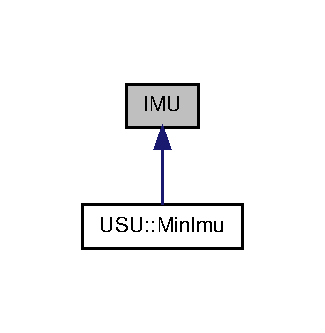
\includegraphics[width=156pt]{class_i_m_u__inherit__graph}
\end{center}
\end{figure}
\subsection*{\-Public \-Member \-Functions}
\begin{DoxyCompactItemize}
\item 
virtual \hyperlink{vector_8h_a148efcf3c5319dd8961dbf9f4b846a98}{vector} \hyperlink{class_i_m_u_a52359006a1ca04d0b1852f374a476f91}{read\-Mag} ()=0
\item 
virtual \hyperlink{vector_8h_a148efcf3c5319dd8961dbf9f4b846a98}{vector} \hyperlink{class_i_m_u_a2928cc8a1fc13464ef90da96fd9358b7}{read\-Acc} ()=0
\item 
virtual \hyperlink{vector_8h_a148efcf3c5319dd8961dbf9f4b846a98}{vector} \hyperlink{class_i_m_u_a887a00b7e1c998a65ee42b021b59d84c}{read\-Gyro} ()=0
\item 
void \hyperlink{class_i_m_u_a1de4cb31f28f71d7cc8b1546ea59b4ab}{read} ()
\item 
virtual void \hyperlink{class_i_m_u_a58899f2357a00a4d1f3b892b879e1e92}{enable} ()=0
\end{DoxyCompactItemize}
\subsection*{\-Public \-Attributes}
\begin{DoxyCompactItemize}
\item 
\hyperlink{vector_8h_ab7556a9a18d16f7b329e566620871c95}{int\-\_\-vector} \hyperlink{class_i_m_u_ad822d0a58bd3050a42cd377453521b5f}{raw\-\_\-m}
\item 
\hyperlink{vector_8h_ab7556a9a18d16f7b329e566620871c95}{int\-\_\-vector} \hyperlink{class_i_m_u_acd6307b0f4f44bd6f057cd8f85080668}{raw\-\_\-a}
\item 
\hyperlink{vector_8h_ab7556a9a18d16f7b329e566620871c95}{int\-\_\-vector} \hyperlink{class_i_m_u_aa63b8395ba841c899a926fc47d4a2435}{raw\-\_\-g}
\end{DoxyCompactItemize}


\subsection{\-Detailed \-Description}
\-Virtual base class for \hyperlink{class_i_m_u}{\-I\-M\-U}. 

\-Derive this class to make your own \-I\-M\-U-\/class. 

\-Definition at line 13 of file \-I\-M\-U.\-h.



\subsection{\-Member \-Function \-Documentation}
\hypertarget{class_i_m_u_a58899f2357a00a4d1f3b892b879e1e92}{\index{\-I\-M\-U@{\-I\-M\-U}!enable@{enable}}
\index{enable@{enable}!IMU@{\-I\-M\-U}}
\subsubsection[{enable}]{\setlength{\rightskip}{0pt plus 5cm}virtual void {\bf \-I\-M\-U\-::enable} (
\begin{DoxyParamCaption}
{}
\end{DoxyParamCaption}
)\hspace{0.3cm}{\ttfamily  \mbox{[}pure virtual\mbox{]}}}}\label{class_i_m_u_a58899f2357a00a4d1f3b892b879e1e92}


\-Implemented in \hyperlink{class_u_s_u_1_1_min_imu_a8f6842375bddcd750203e860b1475a32}{\-U\-S\-U\-::\-Min\-Imu}.

\hypertarget{class_i_m_u_a1de4cb31f28f71d7cc8b1546ea59b4ab}{\index{\-I\-M\-U@{\-I\-M\-U}!read@{read}}
\index{read@{read}!IMU@{\-I\-M\-U}}
\subsubsection[{read}]{\setlength{\rightskip}{0pt plus 5cm}void {\bf \-I\-M\-U\-::read} (
\begin{DoxyParamCaption}
{}
\end{DoxyParamCaption}
)\hspace{0.3cm}{\ttfamily  \mbox{[}inline\mbox{]}}}}\label{class_i_m_u_a1de4cb31f28f71d7cc8b1546ea59b4ab}


\-Definition at line 19 of file \-I\-M\-U.\-h.

\hypertarget{class_i_m_u_a2928cc8a1fc13464ef90da96fd9358b7}{\index{\-I\-M\-U@{\-I\-M\-U}!read\-Acc@{read\-Acc}}
\index{read\-Acc@{read\-Acc}!IMU@{\-I\-M\-U}}
\subsubsection[{read\-Acc}]{\setlength{\rightskip}{0pt plus 5cm}virtual {\bf vector} {\bf \-I\-M\-U\-::read\-Acc} (
\begin{DoxyParamCaption}
{}
\end{DoxyParamCaption}
)\hspace{0.3cm}{\ttfamily  \mbox{[}pure virtual\mbox{]}}}}\label{class_i_m_u_a2928cc8a1fc13464ef90da96fd9358b7}


\-Implemented in \hyperlink{class_u_s_u_1_1_min_imu_ac31e697b05053c7535140eabf4f6f06f}{\-U\-S\-U\-::\-Min\-Imu}.

\hypertarget{class_i_m_u_a887a00b7e1c998a65ee42b021b59d84c}{\index{\-I\-M\-U@{\-I\-M\-U}!read\-Gyro@{read\-Gyro}}
\index{read\-Gyro@{read\-Gyro}!IMU@{\-I\-M\-U}}
\subsubsection[{read\-Gyro}]{\setlength{\rightskip}{0pt plus 5cm}virtual {\bf vector} {\bf \-I\-M\-U\-::read\-Gyro} (
\begin{DoxyParamCaption}
{}
\end{DoxyParamCaption}
)\hspace{0.3cm}{\ttfamily  \mbox{[}pure virtual\mbox{]}}}}\label{class_i_m_u_a887a00b7e1c998a65ee42b021b59d84c}


\-Implemented in \hyperlink{class_u_s_u_1_1_min_imu_a08d89ce9548722810df43bd8439372ff}{\-U\-S\-U\-::\-Min\-Imu}.

\hypertarget{class_i_m_u_a52359006a1ca04d0b1852f374a476f91}{\index{\-I\-M\-U@{\-I\-M\-U}!read\-Mag@{read\-Mag}}
\index{read\-Mag@{read\-Mag}!IMU@{\-I\-M\-U}}
\subsubsection[{read\-Mag}]{\setlength{\rightskip}{0pt plus 5cm}virtual {\bf vector} {\bf \-I\-M\-U\-::read\-Mag} (
\begin{DoxyParamCaption}
{}
\end{DoxyParamCaption}
)\hspace{0.3cm}{\ttfamily  \mbox{[}pure virtual\mbox{]}}}}\label{class_i_m_u_a52359006a1ca04d0b1852f374a476f91}


\-Implemented in \hyperlink{class_u_s_u_1_1_min_imu_add98c9a8e002a56ccb4978079ac2dbfe}{\-U\-S\-U\-::\-Min\-Imu}.



\subsection{\-Member \-Data \-Documentation}
\hypertarget{class_i_m_u_acd6307b0f4f44bd6f057cd8f85080668}{\index{\-I\-M\-U@{\-I\-M\-U}!raw\-\_\-a@{raw\-\_\-a}}
\index{raw\-\_\-a@{raw\-\_\-a}!IMU@{\-I\-M\-U}}
\subsubsection[{raw\-\_\-a}]{\setlength{\rightskip}{0pt plus 5cm}{\bf int\-\_\-vector} {\bf \-I\-M\-U\-::raw\-\_\-a}}}\label{class_i_m_u_acd6307b0f4f44bd6f057cd8f85080668}


\-Definition at line 29 of file \-I\-M\-U.\-h.

\hypertarget{class_i_m_u_aa63b8395ba841c899a926fc47d4a2435}{\index{\-I\-M\-U@{\-I\-M\-U}!raw\-\_\-g@{raw\-\_\-g}}
\index{raw\-\_\-g@{raw\-\_\-g}!IMU@{\-I\-M\-U}}
\subsubsection[{raw\-\_\-g}]{\setlength{\rightskip}{0pt plus 5cm}{\bf int\-\_\-vector} {\bf \-I\-M\-U\-::raw\-\_\-g}}}\label{class_i_m_u_aa63b8395ba841c899a926fc47d4a2435}


\-Definition at line 29 of file \-I\-M\-U.\-h.

\hypertarget{class_i_m_u_ad822d0a58bd3050a42cd377453521b5f}{\index{\-I\-M\-U@{\-I\-M\-U}!raw\-\_\-m@{raw\-\_\-m}}
\index{raw\-\_\-m@{raw\-\_\-m}!IMU@{\-I\-M\-U}}
\subsubsection[{raw\-\_\-m}]{\setlength{\rightskip}{0pt plus 5cm}{\bf int\-\_\-vector} {\bf \-I\-M\-U\-::raw\-\_\-m}}}\label{class_i_m_u_ad822d0a58bd3050a42cd377453521b5f}


\-Definition at line 29 of file \-I\-M\-U.\-h.



\-The documentation for this class was generated from the following file\-:\begin{DoxyCompactItemize}
\item 
include/\hyperlink{_i_m_u_8h}{\-I\-M\-U.\-h}\end{DoxyCompactItemize}

\hypertarget{class_u_s_u_1_1_kalman_filter}{\section{\-U\-S\-U\-:\-:\-Kalman\-Filter \-Class \-Reference}
\label{class_u_s_u_1_1_kalman_filter}\index{\-U\-S\-U\-::\-Kalman\-Filter@{\-U\-S\-U\-::\-Kalman\-Filter}}
}


\-Represents the \-Periodic \-Thread class for state estimation.  




{\ttfamily \#include $<$kalmanfilter.\-h$>$}



\-Inheritance diagram for \-U\-S\-U\-:\-:\-Kalman\-Filter\-:\nopagebreak
\begin{figure}[H]
\begin{center}
\leavevmode
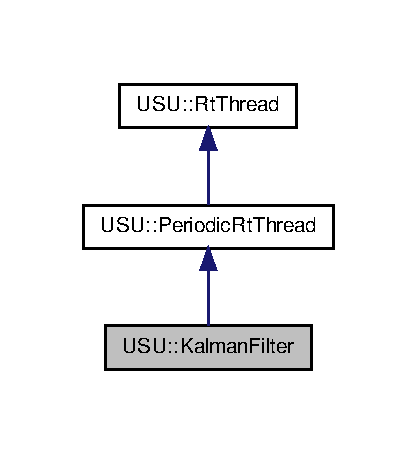
\includegraphics[width=200pt]{class_u_s_u_1_1_kalman_filter__inherit__graph}
\end{center}
\end{figure}


\-Collaboration diagram for \-U\-S\-U\-:\-:\-Kalman\-Filter\-:\nopagebreak
\begin{figure}[H]
\begin{center}
\leavevmode
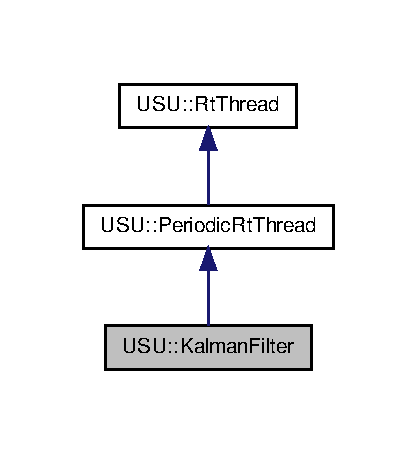
\includegraphics[width=200pt]{class_u_s_u_1_1_kalman_filter__coll__graph}
\end{center}
\end{figure}
\subsection*{\-Public \-Member \-Functions}
\begin{DoxyCompactItemize}
\item 
\hyperlink{class_u_s_u_1_1_kalman_filter_acbde9bd0fafa0e6c1aa078d392b28a6d}{\-Kalman\-Filter} (int priority, unsigned int period\-\_\-us, char $\ast$i2c\-Bus)
\begin{DoxyCompactList}\small\item\em \-Constructor of the class. \end{DoxyCompactList}\item 
virtual void \hyperlink{class_u_s_u_1_1_kalman_filter_a47cc7f620b57b25133289e61dbf2a7be}{run} ()
\begin{DoxyCompactList}\small\item\em \-Thread routine. \end{DoxyCompactList}\item 
void \hyperlink{class_u_s_u_1_1_kalman_filter_a3f8b3ce719dcb24745150f8c4ef361b8}{stop} ()
\begin{DoxyCompactList}\small\item\em \-Signals the thread to stop. \end{DoxyCompactList}\item 
bool \hyperlink{class_u_s_u_1_1_kalman_filter_a3ed1c15b5301f0840f6a7a3d7696fb0a}{get\-State} ()
\begin{DoxyCompactList}\small\item\em \-Returns the current system state estimate. \end{DoxyCompactList}\end{DoxyCompactItemize}


\subsection{\-Detailed \-Description}
\-Represents the \-Periodic \-Thread class for state estimation. 

\-This class is derived from \hyperlink{class_u_s_u_1_1_periodic_rt_thread}{\-Periodic\-Rt\-Thread}. \-It initializes the interface to the \-Min\-I\-M\-U9v2 and estimates the system state using \-Kalman filtering techniques. \-The state estimate can be accessed from other threads (protected by mutex).

\-T\-O\-D\-O\-:
\begin{DoxyItemize}
\item \-Add interface to 3\-D\-M-\/\-G\-X3-\/25
\item \-Add interface to star camera 
\end{DoxyItemize}

\-Definition at line 37 of file kalmanfilter.\-h.



\subsection{\-Constructor \& \-Destructor \-Documentation}
\hypertarget{class_u_s_u_1_1_kalman_filter_acbde9bd0fafa0e6c1aa078d392b28a6d}{\index{\-U\-S\-U\-::\-Kalman\-Filter@{\-U\-S\-U\-::\-Kalman\-Filter}!\-Kalman\-Filter@{\-Kalman\-Filter}}
\index{\-Kalman\-Filter@{\-Kalman\-Filter}!USU::KalmanFilter@{\-U\-S\-U\-::\-Kalman\-Filter}}
\subsubsection[{\-Kalman\-Filter}]{\setlength{\rightskip}{0pt plus 5cm}{\bf \-Kalman\-Filter\-::\-Kalman\-Filter} (
\begin{DoxyParamCaption}
\item[{int}]{priority, }
\item[{unsigned int}]{period\-\_\-us, }
\item[{char $\ast$}]{i2c\-Bus}
\end{DoxyParamCaption}
)}}\label{class_u_s_u_1_1_kalman_filter_acbde9bd0fafa0e6c1aa078d392b28a6d}


\-Constructor of the class. 

\-Initializes the interface to the \-Min\-I\-M\-U9 sensors


\begin{DoxyParams}{\-Parameters}
{\em priority} & priority of the underlying periodic thread \\
\hline
{\em period\-\_\-us} & period (in us) of the underlying periodic thread \\
\hline
{\em i2c\-Bus} & name of the \-I2\-C-\/device (e.\-g. /dev/i2c-\/1) \\
\hline
\end{DoxyParams}


\-Definition at line 47 of file kalmanfilter.\-cpp.



\subsection{\-Member \-Function \-Documentation}
\hypertarget{class_u_s_u_1_1_kalman_filter_a3ed1c15b5301f0840f6a7a3d7696fb0a}{\index{\-U\-S\-U\-::\-Kalman\-Filter@{\-U\-S\-U\-::\-Kalman\-Filter}!get\-State@{get\-State}}
\index{get\-State@{get\-State}!USU::KalmanFilter@{\-U\-S\-U\-::\-Kalman\-Filter}}
\subsubsection[{get\-State}]{\setlength{\rightskip}{0pt plus 5cm}bool {\bf \-Kalman\-Filter\-::get\-State} (
\begin{DoxyParamCaption}
{}
\end{DoxyParamCaption}
)}}\label{class_u_s_u_1_1_kalman_filter_a3ed1c15b5301f0840f6a7a3d7696fb0a}


\-Returns the current system state estimate. 

\-Copies the current system state estimate. \-Acquires mutex before acessing the internal variable to avoid read/write-\/conflicts.

\begin{DoxyReturn}{\-Returns}
bool \-Current system state \-T\-O\-D\-O\-: \-Currently only dummy variable. \-Replace with actual state representation (quaternion?) 
\end{DoxyReturn}


\-Definition at line 118 of file kalmanfilter.\-cpp.

\hypertarget{class_u_s_u_1_1_kalman_filter_a47cc7f620b57b25133289e61dbf2a7be}{\index{\-U\-S\-U\-::\-Kalman\-Filter@{\-U\-S\-U\-::\-Kalman\-Filter}!run@{run}}
\index{run@{run}!USU::KalmanFilter@{\-U\-S\-U\-::\-Kalman\-Filter}}
\subsubsection[{run}]{\setlength{\rightskip}{0pt plus 5cm}void {\bf \-Kalman\-Filter\-::run} (
\begin{DoxyParamCaption}
{}
\end{DoxyParamCaption}
)\hspace{0.3cm}{\ttfamily  \mbox{[}virtual\mbox{]}}}}\label{class_u_s_u_1_1_kalman_filter_a47cc7f620b57b25133289e61dbf2a7be}


\-Thread routine. 


\begin{DoxyItemize}
\item \-Gets sensor data from \-Min\-I\-M\-U9
\item \-Calculate state estimate
\item wait for next timer event
\end{DoxyItemize}

\-T\-O\-D\-O\-: \-Its only an idea no actual implementation yet. \-T\-O\-D\-O\-: \-Do some \-Kalman-\/\-Filtering magic here

\-T\-O\-D\-O\-: some more magic 

\-Implements \hyperlink{class_u_s_u_1_1_periodic_rt_thread_ac9146b3088a9b268594ce41d002d020a}{\-U\-S\-U\-::\-Periodic\-Rt\-Thread}.



\-Definition at line 53 of file kalmanfilter.\-cpp.

\hypertarget{class_u_s_u_1_1_kalman_filter_a3f8b3ce719dcb24745150f8c4ef361b8}{\index{\-U\-S\-U\-::\-Kalman\-Filter@{\-U\-S\-U\-::\-Kalman\-Filter}!stop@{stop}}
\index{stop@{stop}!USU::KalmanFilter@{\-U\-S\-U\-::\-Kalman\-Filter}}
\subsubsection[{stop}]{\setlength{\rightskip}{0pt plus 5cm}void {\bf \-U\-S\-U\-::\-Kalman\-Filter\-::stop} (
\begin{DoxyParamCaption}
{}
\end{DoxyParamCaption}
)\hspace{0.3cm}{\ttfamily  \mbox{[}inline\mbox{]}}}}\label{class_u_s_u_1_1_kalman_filter_a3f8b3ce719dcb24745150f8c4ef361b8}


\-Signals the thread to stop. 



\-Definition at line 66 of file kalmanfilter.\-h.



\-The documentation for this class was generated from the following files\-:\begin{DoxyCompactItemize}
\item 
\hyperlink{kalmanfilter_8h}{kalmanfilter.\-h}\item 
\hyperlink{kalmanfilter_8cpp}{kalmanfilter.\-cpp}\end{DoxyCompactItemize}

\hypertarget{class_l3_g}{\section{\-L3\-G \-Class \-Reference}
\label{class_l3_g}\index{\-L3\-G@{\-L3\-G}}
}


{\ttfamily \#include $<$\-L3\-G.\-h$>$}

\subsection*{\-Public \-Member \-Functions}
\begin{DoxyCompactItemize}
\item 
\hyperlink{class_l3_g_a98c77b59983763302f3b9fde5b284a33}{\-L3\-G} (const char $\ast$i2c\-Device\-Name)
\item 
void \hyperlink{class_l3_g_a48decd4910020dc16c219e0081239c45}{enable} (void)
\item 
void \hyperlink{class_l3_g_a6ab0e9d8b8349eb08ba97432660c258e}{write\-Reg} (uint8\-\_\-t reg, uint8\-\_\-t value)
\item 
uint8\-\_\-t \hyperlink{class_l3_g_a5791e06a4e63a54300716780818ed726}{read\-Reg} (uint8\-\_\-t reg)
\item 
void \hyperlink{class_l3_g_a4b1913429824dc07bd2017c3755e7985}{read} ()
\end{DoxyCompactItemize}
\subsection*{\-Public \-Attributes}
\begin{DoxyCompactItemize}
\item 
int \hyperlink{class_l3_g_a0cb874e50a2ea4753d81e9a46c7e45ce}{g} \mbox{[}3\mbox{]}
\end{DoxyCompactItemize}


\subsection{\-Detailed \-Description}


\-Definition at line 37 of file \-L3\-G.\-h.



\subsection{\-Constructor \& \-Destructor \-Documentation}
\hypertarget{class_l3_g_a98c77b59983763302f3b9fde5b284a33}{\index{\-L3\-G@{\-L3\-G}!\-L3\-G@{\-L3\-G}}
\index{\-L3\-G@{\-L3\-G}!L3G@{\-L3\-G}}
\subsubsection[{\-L3\-G}]{\setlength{\rightskip}{0pt plus 5cm}{\bf \-L3\-G\-::\-L3\-G} (
\begin{DoxyParamCaption}
\item[{const char $\ast$}]{i2c\-Device\-Name}
\end{DoxyParamCaption}
)}}\label{class_l3_g_a98c77b59983763302f3b9fde5b284a33}


\-Definition at line 9 of file \-L3\-G.\-cpp.



\subsection{\-Member \-Function \-Documentation}
\hypertarget{class_l3_g_a48decd4910020dc16c219e0081239c45}{\index{\-L3\-G@{\-L3\-G}!enable@{enable}}
\index{enable@{enable}!L3G@{\-L3\-G}}
\subsubsection[{enable}]{\setlength{\rightskip}{0pt plus 5cm}void {\bf \-L3\-G\-::enable} (
\begin{DoxyParamCaption}
\item[{void}]{}
\end{DoxyParamCaption}
)}}\label{class_l3_g_a48decd4910020dc16c219e0081239c45}


\-Definition at line 29 of file \-L3\-G.\-cpp.

\hypertarget{class_l3_g_a4b1913429824dc07bd2017c3755e7985}{\index{\-L3\-G@{\-L3\-G}!read@{read}}
\index{read@{read}!L3G@{\-L3\-G}}
\subsubsection[{read}]{\setlength{\rightskip}{0pt plus 5cm}void {\bf \-L3\-G\-::read} (
\begin{DoxyParamCaption}
{}
\end{DoxyParamCaption}
)}}\label{class_l3_g_a4b1913429824dc07bd2017c3755e7985}


\-Definition at line 45 of file \-L3\-G.\-cpp.

\hypertarget{class_l3_g_a5791e06a4e63a54300716780818ed726}{\index{\-L3\-G@{\-L3\-G}!read\-Reg@{read\-Reg}}
\index{read\-Reg@{read\-Reg}!L3G@{\-L3\-G}}
\subsubsection[{read\-Reg}]{\setlength{\rightskip}{0pt plus 5cm}uint8\-\_\-t {\bf \-L3\-G\-::read\-Reg} (
\begin{DoxyParamCaption}
\item[{uint8\-\_\-t}]{reg}
\end{DoxyParamCaption}
)}}\label{class_l3_g_a5791e06a4e63a54300716780818ed726}


\-Definition at line 40 of file \-L3\-G.\-cpp.

\hypertarget{class_l3_g_a6ab0e9d8b8349eb08ba97432660c258e}{\index{\-L3\-G@{\-L3\-G}!write\-Reg@{write\-Reg}}
\index{write\-Reg@{write\-Reg}!L3G@{\-L3\-G}}
\subsubsection[{write\-Reg}]{\setlength{\rightskip}{0pt plus 5cm}void {\bf \-L3\-G\-::write\-Reg} (
\begin{DoxyParamCaption}
\item[{uint8\-\_\-t}]{reg, }
\item[{uint8\-\_\-t}]{value}
\end{DoxyParamCaption}
)}}\label{class_l3_g_a6ab0e9d8b8349eb08ba97432660c258e}


\-Definition at line 35 of file \-L3\-G.\-cpp.



\subsection{\-Member \-Data \-Documentation}
\hypertarget{class_l3_g_a0cb874e50a2ea4753d81e9a46c7e45ce}{\index{\-L3\-G@{\-L3\-G}!g@{g}}
\index{g@{g}!L3G@{\-L3\-G}}
\subsubsection[{g}]{\setlength{\rightskip}{0pt plus 5cm}int {\bf \-L3\-G\-::g}\mbox{[}3\mbox{]}}}\label{class_l3_g_a0cb874e50a2ea4753d81e9a46c7e45ce}


\-Definition at line 43 of file \-L3\-G.\-h.



\-The documentation for this class was generated from the following files\-:\begin{DoxyCompactItemize}
\item 
include/\hyperlink{_l3_g_8h}{\-L3\-G.\-h}\item 
src/\hyperlink{_l3_g_8cpp}{\-L3\-G.\-cpp}\end{DoxyCompactItemize}

\hypertarget{class_u_s_u_1_1_lock}{\section{\-U\-S\-U\-:\-:\-Lock \-Class \-Reference}
\label{class_u_s_u_1_1_lock}\index{\-U\-S\-U\-::\-Lock@{\-U\-S\-U\-::\-Lock}}
}


\-Wrapper class for pthread mutexes.  




{\ttfamily \#include $<$\-Lock.\-h$>$}

\subsection*{\-Public \-Member \-Functions}
\begin{DoxyCompactItemize}
\item 
\hyperlink{class_u_s_u_1_1_lock_a4eb7425055400e6edf40c09b89a3b4c8}{\-Lock} ()
\item 
virtual \hyperlink{class_u_s_u_1_1_lock_a81280a2e319eab2bf18d9eebb591d871}{$\sim$\-Lock} ()
\item 
void \hyperlink{class_u_s_u_1_1_lock_a68790e92c297da5b067f0b9797a1a9f0}{lock} ()
\item 
void \hyperlink{class_u_s_u_1_1_lock_a77d54adab825e5532c8bd38f642fdd89}{unlock} ()
\end{DoxyCompactItemize}


\subsection{\-Detailed \-Description}
\-Wrapper class for pthread mutexes. 

\-T\-O\-D\-O\-: use exceptions 

\-Definition at line 24 of file \-Lock.\-h.



\subsection{\-Constructor \& \-Destructor \-Documentation}
\hypertarget{class_u_s_u_1_1_lock_a4eb7425055400e6edf40c09b89a3b4c8}{\index{\-U\-S\-U\-::\-Lock@{\-U\-S\-U\-::\-Lock}!\-Lock@{\-Lock}}
\index{\-Lock@{\-Lock}!USU::Lock@{\-U\-S\-U\-::\-Lock}}
\subsubsection[{\-Lock}]{\setlength{\rightskip}{0pt plus 5cm}\-U\-S\-U\-::\-Lock\-::\-Lock (
\begin{DoxyParamCaption}
{}
\end{DoxyParamCaption}
)\hspace{0.3cm}{\ttfamily  \mbox{[}inline\mbox{]}}}}\label{class_u_s_u_1_1_lock_a4eb7425055400e6edf40c09b89a3b4c8}
\-Constructor\-: \-Creates the pthread-\/mutex 

\-Definition at line 47 of file \-Lock.\-h.

\hypertarget{class_u_s_u_1_1_lock_a81280a2e319eab2bf18d9eebb591d871}{\index{\-U\-S\-U\-::\-Lock@{\-U\-S\-U\-::\-Lock}!$\sim$\-Lock@{$\sim$\-Lock}}
\index{$\sim$\-Lock@{$\sim$\-Lock}!USU::Lock@{\-U\-S\-U\-::\-Lock}}
\subsubsection[{$\sim$\-Lock}]{\setlength{\rightskip}{0pt plus 5cm}{\bf \-U\-S\-U\-::\-Lock\-::$\sim$\-Lock} (
\begin{DoxyParamCaption}
{}
\end{DoxyParamCaption}
)\hspace{0.3cm}{\ttfamily  \mbox{[}inline, virtual\mbox{]}}}}\label{class_u_s_u_1_1_lock_a81280a2e319eab2bf18d9eebb591d871}
\-Destructor\-: \-Frees the pthread-\/mutex 

\-Definition at line 57 of file \-Lock.\-h.



\subsection{\-Member \-Function \-Documentation}
\hypertarget{class_u_s_u_1_1_lock_a68790e92c297da5b067f0b9797a1a9f0}{\index{\-U\-S\-U\-::\-Lock@{\-U\-S\-U\-::\-Lock}!lock@{lock}}
\index{lock@{lock}!USU::Lock@{\-U\-S\-U\-::\-Lock}}
\subsubsection[{lock}]{\setlength{\rightskip}{0pt plus 5cm}void {\bf \-U\-S\-U\-::\-Lock\-::lock} (
\begin{DoxyParamCaption}
{}
\end{DoxyParamCaption}
)\hspace{0.3cm}{\ttfamily  \mbox{[}inline\mbox{]}}}}\label{class_u_s_u_1_1_lock_a68790e92c297da5b067f0b9797a1a9f0}
\-Locks the mutex 

\-Definition at line 68 of file \-Lock.\-h.

\hypertarget{class_u_s_u_1_1_lock_a77d54adab825e5532c8bd38f642fdd89}{\index{\-U\-S\-U\-::\-Lock@{\-U\-S\-U\-::\-Lock}!unlock@{unlock}}
\index{unlock@{unlock}!USU::Lock@{\-U\-S\-U\-::\-Lock}}
\subsubsection[{unlock}]{\setlength{\rightskip}{0pt plus 5cm}void {\bf \-U\-S\-U\-::\-Lock\-::unlock} (
\begin{DoxyParamCaption}
{}
\end{DoxyParamCaption}
)\hspace{0.3cm}{\ttfamily  \mbox{[}inline\mbox{]}}}}\label{class_u_s_u_1_1_lock_a77d54adab825e5532c8bd38f642fdd89}
\-Unlocks the mutex 

\-Definition at line 74 of file \-Lock.\-h.



\-The documentation for this class was generated from the following file\-:\begin{DoxyCompactItemize}
\item 
include/\hyperlink{_lock_8h}{\-Lock.\-h}\end{DoxyCompactItemize}

\hypertarget{class_l_s_m303}{\section{\-L\-S\-M303 \-Class \-Reference}
\label{class_l_s_m303}\index{\-L\-S\-M303@{\-L\-S\-M303}}
}


{\ttfamily \#include $<$\-L\-S\-M303.\-h$>$}

\subsection*{\-Public \-Member \-Functions}
\begin{DoxyCompactItemize}
\item 
\hyperlink{class_l_s_m303_a372710f74d63e809ef08348d919a2842}{\-L\-S\-M303} (const char $\ast$i2c\-Device\-Name)
\item 
void \hyperlink{class_l_s_m303_af2c1baa290df19e7cd4667a13a68a19a}{enable} (void)
\item 
void \hyperlink{class_l_s_m303_a3baf5341cf9d7d789b81b1cec7e81f12}{write\-Acc\-Reg} (uint8\-\_\-t reg, uint8\-\_\-t value)
\item 
uint8\-\_\-t \hyperlink{class_l_s_m303_a26ba086aec95c01c05e6b980383d1ed9}{read\-Acc\-Reg} (uint8\-\_\-t reg)
\item 
void \hyperlink{class_l_s_m303_a70b49953d20ff311bc23dfa8c1ec7a4f}{write\-Mag\-Reg} (uint8\-\_\-t reg, uint8\-\_\-t value)
\item 
uint8\-\_\-t \hyperlink{class_l_s_m303_a5d6d0b492501b76b7fde821036205bda}{read\-Mag\-Reg} (uint8\-\_\-t reg)
\item 
void \hyperlink{class_l_s_m303_ac1396a51b288eadc41fd19fbd79ef68e}{read\-Acc} (void)
\item 
void \hyperlink{class_l_s_m303_abc93e8d8101c6b00df2ae85c5f8ded9e}{read\-Mag} (void)
\item 
void \hyperlink{class_l_s_m303_a9f40456878f534bba32490d19f3a64ce}{read} (void)
\end{DoxyCompactItemize}
\subsection*{\-Public \-Attributes}
\begin{DoxyCompactItemize}
\item 
int \hyperlink{class_l_s_m303_ad71c39fa2c1dfd978c9e93b48a6a9310}{a} \mbox{[}3\mbox{]}
\item 
int \hyperlink{class_l_s_m303_a606cb6a86d385c4c4a9767f6b1bf2ea5}{m} \mbox{[}3\mbox{]}
\end{DoxyCompactItemize}


\subsection{\-Detailed \-Description}


\-Definition at line 78 of file \-L\-S\-M303.\-h.



\subsection{\-Constructor \& \-Destructor \-Documentation}
\hypertarget{class_l_s_m303_a372710f74d63e809ef08348d919a2842}{\index{\-L\-S\-M303@{\-L\-S\-M303}!\-L\-S\-M303@{\-L\-S\-M303}}
\index{\-L\-S\-M303@{\-L\-S\-M303}!LSM303@{\-L\-S\-M303}}
\subsubsection[{\-L\-S\-M303}]{\setlength{\rightskip}{0pt plus 5cm}{\bf \-L\-S\-M303\-::\-L\-S\-M303} (
\begin{DoxyParamCaption}
\item[{const char $\ast$}]{i2c\-Device\-Name}
\end{DoxyParamCaption}
)}}\label{class_l_s_m303_a372710f74d63e809ef08348d919a2842}


\-Definition at line 22 of file \-L\-S\-M303.\-cpp.



\subsection{\-Member \-Function \-Documentation}
\hypertarget{class_l_s_m303_af2c1baa290df19e7cd4667a13a68a19a}{\index{\-L\-S\-M303@{\-L\-S\-M303}!enable@{enable}}
\index{enable@{enable}!LSM303@{\-L\-S\-M303}}
\subsubsection[{enable}]{\setlength{\rightskip}{0pt plus 5cm}void {\bf \-L\-S\-M303\-::enable} (
\begin{DoxyParamCaption}
\item[{void}]{}
\end{DoxyParamCaption}
)}}\label{class_l_s_m303_af2c1baa290df19e7cd4667a13a68a19a}


\-Definition at line 73 of file \-L\-S\-M303.\-cpp.

\hypertarget{class_l_s_m303_a9f40456878f534bba32490d19f3a64ce}{\index{\-L\-S\-M303@{\-L\-S\-M303}!read@{read}}
\index{read@{read}!LSM303@{\-L\-S\-M303}}
\subsubsection[{read}]{\setlength{\rightskip}{0pt plus 5cm}void {\bf \-L\-S\-M303\-::read} (
\begin{DoxyParamCaption}
\item[{void}]{}
\end{DoxyParamCaption}
)}}\label{class_l_s_m303_a9f40456878f534bba32490d19f3a64ce}


\-Definition at line 118 of file \-L\-S\-M303.\-cpp.

\hypertarget{class_l_s_m303_ac1396a51b288eadc41fd19fbd79ef68e}{\index{\-L\-S\-M303@{\-L\-S\-M303}!read\-Acc@{read\-Acc}}
\index{read\-Acc@{read\-Acc}!LSM303@{\-L\-S\-M303}}
\subsubsection[{read\-Acc}]{\setlength{\rightskip}{0pt plus 5cm}void {\bf \-L\-S\-M303\-::read\-Acc} (
\begin{DoxyParamCaption}
\item[{void}]{}
\end{DoxyParamCaption}
)}}\label{class_l_s_m303_ac1396a51b288eadc41fd19fbd79ef68e}


\-Definition at line 93 of file \-L\-S\-M303.\-cpp.

\hypertarget{class_l_s_m303_a26ba086aec95c01c05e6b980383d1ed9}{\index{\-L\-S\-M303@{\-L\-S\-M303}!read\-Acc\-Reg@{read\-Acc\-Reg}}
\index{read\-Acc\-Reg@{read\-Acc\-Reg}!LSM303@{\-L\-S\-M303}}
\subsubsection[{read\-Acc\-Reg}]{\setlength{\rightskip}{0pt plus 5cm}uint8\-\_\-t {\bf \-L\-S\-M303\-::read\-Acc\-Reg} (
\begin{DoxyParamCaption}
\item[{uint8\-\_\-t}]{reg}
\end{DoxyParamCaption}
)}}\label{class_l_s_m303_a26ba086aec95c01c05e6b980383d1ed9}


\-Definition at line 56 of file \-L\-S\-M303.\-cpp.

\hypertarget{class_l_s_m303_abc93e8d8101c6b00df2ae85c5f8ded9e}{\index{\-L\-S\-M303@{\-L\-S\-M303}!read\-Mag@{read\-Mag}}
\index{read\-Mag@{read\-Mag}!LSM303@{\-L\-S\-M303}}
\subsubsection[{read\-Mag}]{\setlength{\rightskip}{0pt plus 5cm}void {\bf \-L\-S\-M303\-::read\-Mag} (
\begin{DoxyParamCaption}
\item[{void}]{}
\end{DoxyParamCaption}
)}}\label{class_l_s_m303_abc93e8d8101c6b00df2ae85c5f8ded9e}


\-Definition at line 103 of file \-L\-S\-M303.\-cpp.

\hypertarget{class_l_s_m303_a5d6d0b492501b76b7fde821036205bda}{\index{\-L\-S\-M303@{\-L\-S\-M303}!read\-Mag\-Reg@{read\-Mag\-Reg}}
\index{read\-Mag\-Reg@{read\-Mag\-Reg}!LSM303@{\-L\-S\-M303}}
\subsubsection[{read\-Mag\-Reg}]{\setlength{\rightskip}{0pt plus 5cm}uint8\-\_\-t {\bf \-L\-S\-M303\-::read\-Mag\-Reg} (
\begin{DoxyParamCaption}
\item[{uint8\-\_\-t}]{reg}
\end{DoxyParamCaption}
)}}\label{class_l_s_m303_a5d6d0b492501b76b7fde821036205bda}


\-Definition at line 51 of file \-L\-S\-M303.\-cpp.

\hypertarget{class_l_s_m303_a3baf5341cf9d7d789b81b1cec7e81f12}{\index{\-L\-S\-M303@{\-L\-S\-M303}!write\-Acc\-Reg@{write\-Acc\-Reg}}
\index{write\-Acc\-Reg@{write\-Acc\-Reg}!LSM303@{\-L\-S\-M303}}
\subsubsection[{write\-Acc\-Reg}]{\setlength{\rightskip}{0pt plus 5cm}void {\bf \-L\-S\-M303\-::write\-Acc\-Reg} (
\begin{DoxyParamCaption}
\item[{uint8\-\_\-t}]{reg, }
\item[{uint8\-\_\-t}]{value}
\end{DoxyParamCaption}
)}}\label{class_l_s_m303_a3baf5341cf9d7d789b81b1cec7e81f12}


\-Definition at line 66 of file \-L\-S\-M303.\-cpp.

\hypertarget{class_l_s_m303_a70b49953d20ff311bc23dfa8c1ec7a4f}{\index{\-L\-S\-M303@{\-L\-S\-M303}!write\-Mag\-Reg@{write\-Mag\-Reg}}
\index{write\-Mag\-Reg@{write\-Mag\-Reg}!LSM303@{\-L\-S\-M303}}
\subsubsection[{write\-Mag\-Reg}]{\setlength{\rightskip}{0pt plus 5cm}void {\bf \-L\-S\-M303\-::write\-Mag\-Reg} (
\begin{DoxyParamCaption}
\item[{uint8\-\_\-t}]{reg, }
\item[{uint8\-\_\-t}]{value}
\end{DoxyParamCaption}
)}}\label{class_l_s_m303_a70b49953d20ff311bc23dfa8c1ec7a4f}


\-Definition at line 61 of file \-L\-S\-M303.\-cpp.



\subsection{\-Member \-Data \-Documentation}
\hypertarget{class_l_s_m303_ad71c39fa2c1dfd978c9e93b48a6a9310}{\index{\-L\-S\-M303@{\-L\-S\-M303}!a@{a}}
\index{a@{a}!LSM303@{\-L\-S\-M303}}
\subsubsection[{a}]{\setlength{\rightskip}{0pt plus 5cm}int {\bf \-L\-S\-M303\-::a}\mbox{[}3\mbox{]}}}\label{class_l_s_m303_ad71c39fa2c1dfd978c9e93b48a6a9310}


\-Definition at line 81 of file \-L\-S\-M303.\-h.

\hypertarget{class_l_s_m303_a606cb6a86d385c4c4a9767f6b1bf2ea5}{\index{\-L\-S\-M303@{\-L\-S\-M303}!m@{m}}
\index{m@{m}!LSM303@{\-L\-S\-M303}}
\subsubsection[{m}]{\setlength{\rightskip}{0pt plus 5cm}int {\bf \-L\-S\-M303\-::m}\mbox{[}3\mbox{]}}}\label{class_l_s_m303_a606cb6a86d385c4c4a9767f6b1bf2ea5}


\-Definition at line 82 of file \-L\-S\-M303.\-h.



\-The documentation for this class was generated from the following files\-:\begin{DoxyCompactItemize}
\item 
minimu/\hyperlink{_l_s_m303_8h}{\-L\-S\-M303.\-h}\item 
minimu/\hyperlink{_l_s_m303_8cpp}{\-L\-S\-M303.\-cpp}\end{DoxyCompactItemize}

\hypertarget{class_min_imu}{\section{\-Min\-Imu \-Class \-Reference}
\label{class_min_imu}\index{\-Min\-Imu@{\-Min\-Imu}}
}


{\ttfamily \#include $<$minimu.\-h$>$}



\-Inheritance diagram for \-Min\-Imu\-:
\nopagebreak
\begin{figure}[H]
\begin{center}
\leavevmode
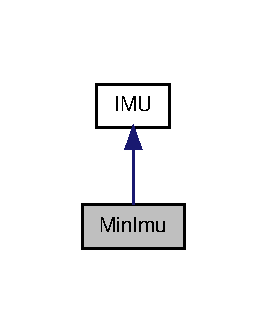
\includegraphics[width=128pt]{class_min_imu__inherit__graph}
\end{center}
\end{figure}


\-Collaboration diagram for \-Min\-Imu\-:
\nopagebreak
\begin{figure}[H]
\begin{center}
\leavevmode
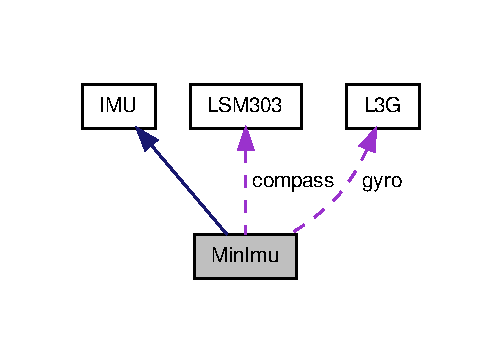
\includegraphics[width=241pt]{class_min_imu__coll__graph}
\end{center}
\end{figure}
\subsection*{\-Public \-Member \-Functions}
\begin{DoxyCompactItemize}
\item 
\hyperlink{class_min_imu_a2584a081b9ed215df6823133f7f010d2}{\-Min\-Imu} (const char $\ast$i2c\-Device\-Name)
\item 
virtual \hyperlink{vector_8h_a148efcf3c5319dd8961dbf9f4b846a98}{vector} \hyperlink{class_min_imu_add98c9a8e002a56ccb4978079ac2dbfe}{read\-Mag} ()
\item 
virtual \hyperlink{vector_8h_a148efcf3c5319dd8961dbf9f4b846a98}{vector} \hyperlink{class_min_imu_ac31e697b05053c7535140eabf4f6f06f}{read\-Acc} ()
\item 
virtual \hyperlink{vector_8h_a148efcf3c5319dd8961dbf9f4b846a98}{vector} \hyperlink{class_min_imu_a08d89ce9548722810df43bd8439372ff}{read\-Gyro} ()
\item 
virtual void \hyperlink{class_min_imu_a8f6842375bddcd750203e860b1475a32}{enable} ()
\end{DoxyCompactItemize}
\subsection*{\-Public \-Attributes}
\begin{DoxyCompactItemize}
\item 
\hyperlink{class_l_s_m303}{\-L\-S\-M303} \hyperlink{class_min_imu_a35f286e23317c02649ce133d60b063e2}{compass}
\item 
\hyperlink{class_l3_g}{\-L3\-G} \hyperlink{class_min_imu_a4d70040f3bc073706b65dbafcf97f7e2}{gyro}
\end{DoxyCompactItemize}


\subsection{\-Detailed \-Description}


\-Definition at line 9 of file minimu.\-h.



\subsection{\-Constructor \& \-Destructor \-Documentation}
\hypertarget{class_min_imu_a2584a081b9ed215df6823133f7f010d2}{\index{\-Min\-Imu@{\-Min\-Imu}!\-Min\-Imu@{\-Min\-Imu}}
\index{\-Min\-Imu@{\-Min\-Imu}!MinImu@{\-Min\-Imu}}
\subsubsection[{\-Min\-Imu}]{\setlength{\rightskip}{0pt plus 5cm}{\bf \-Min\-Imu\-::\-Min\-Imu} (
\begin{DoxyParamCaption}
\item[{const char $\ast$}]{i2c\-Device\-Name}
\end{DoxyParamCaption}
)}}\label{class_min_imu_a2584a081b9ed215df6823133f7f010d2}


\-Definition at line 4 of file minimu.\-cpp.



\subsection{\-Member \-Function \-Documentation}
\hypertarget{class_min_imu_a8f6842375bddcd750203e860b1475a32}{\index{\-Min\-Imu@{\-Min\-Imu}!enable@{enable}}
\index{enable@{enable}!MinImu@{\-Min\-Imu}}
\subsubsection[{enable}]{\setlength{\rightskip}{0pt plus 5cm}void {\bf \-Min\-Imu\-::enable} (
\begin{DoxyParamCaption}
\item[{void}]{}
\end{DoxyParamCaption}
)\hspace{0.3cm}{\ttfamily  \mbox{[}virtual\mbox{]}}}}\label{class_min_imu_a8f6842375bddcd750203e860b1475a32}


\-Implements \hyperlink{class_i_m_u_a58899f2357a00a4d1f3b892b879e1e92}{\-I\-M\-U}.



\-Definition at line 10 of file minimu.\-cpp.

\hypertarget{class_min_imu_ac31e697b05053c7535140eabf4f6f06f}{\index{\-Min\-Imu@{\-Min\-Imu}!read\-Acc@{read\-Acc}}
\index{read\-Acc@{read\-Acc}!MinImu@{\-Min\-Imu}}
\subsubsection[{read\-Acc}]{\setlength{\rightskip}{0pt plus 5cm}{\bf vector} {\bf \-Min\-Imu\-::read\-Acc} (
\begin{DoxyParamCaption}
\item[{void}]{}
\end{DoxyParamCaption}
)\hspace{0.3cm}{\ttfamily  \mbox{[}virtual\mbox{]}}}}\label{class_min_imu_ac31e697b05053c7535140eabf4f6f06f}


\-Implements \hyperlink{class_i_m_u_a2928cc8a1fc13464ef90da96fd9358b7}{\-I\-M\-U}.



\-Definition at line 27 of file minimu.\-cpp.

\hypertarget{class_min_imu_a08d89ce9548722810df43bd8439372ff}{\index{\-Min\-Imu@{\-Min\-Imu}!read\-Gyro@{read\-Gyro}}
\index{read\-Gyro@{read\-Gyro}!MinImu@{\-Min\-Imu}}
\subsubsection[{read\-Gyro}]{\setlength{\rightskip}{0pt plus 5cm}{\bf vector} {\bf \-Min\-Imu\-::read\-Gyro} (
\begin{DoxyParamCaption}
{}
\end{DoxyParamCaption}
)\hspace{0.3cm}{\ttfamily  \mbox{[}virtual\mbox{]}}}}\label{class_min_imu_a08d89ce9548722810df43bd8439372ff}


\-Implements \hyperlink{class_i_m_u_a887a00b7e1c998a65ee42b021b59d84c}{\-I\-M\-U}.



\-Definition at line 16 of file minimu.\-cpp.

\hypertarget{class_min_imu_add98c9a8e002a56ccb4978079ac2dbfe}{\index{\-Min\-Imu@{\-Min\-Imu}!read\-Mag@{read\-Mag}}
\index{read\-Mag@{read\-Mag}!MinImu@{\-Min\-Imu}}
\subsubsection[{read\-Mag}]{\setlength{\rightskip}{0pt plus 5cm}{\bf vector} {\bf \-Min\-Imu\-::read\-Mag} (
\begin{DoxyParamCaption}
\item[{void}]{}
\end{DoxyParamCaption}
)\hspace{0.3cm}{\ttfamily  \mbox{[}virtual\mbox{]}}}}\label{class_min_imu_add98c9a8e002a56ccb4978079ac2dbfe}


\-Implements \hyperlink{class_i_m_u_a52359006a1ca04d0b1852f374a476f91}{\-I\-M\-U}.



\-Definition at line 38 of file minimu.\-cpp.



\subsection{\-Member \-Data \-Documentation}
\hypertarget{class_min_imu_a35f286e23317c02649ce133d60b063e2}{\index{\-Min\-Imu@{\-Min\-Imu}!compass@{compass}}
\index{compass@{compass}!MinImu@{\-Min\-Imu}}
\subsubsection[{compass}]{\setlength{\rightskip}{0pt plus 5cm}{\bf \-L\-S\-M303} {\bf \-Min\-Imu\-::compass}}}\label{class_min_imu_a35f286e23317c02649ce133d60b063e2}


\-Definition at line 12 of file minimu.\-h.

\hypertarget{class_min_imu_a4d70040f3bc073706b65dbafcf97f7e2}{\index{\-Min\-Imu@{\-Min\-Imu}!gyro@{gyro}}
\index{gyro@{gyro}!MinImu@{\-Min\-Imu}}
\subsubsection[{gyro}]{\setlength{\rightskip}{0pt plus 5cm}{\bf \-L3\-G} {\bf \-Min\-Imu\-::gyro}}}\label{class_min_imu_a4d70040f3bc073706b65dbafcf97f7e2}


\-Definition at line 13 of file minimu.\-h.



\-The documentation for this class was generated from the following files\-:\begin{DoxyCompactItemize}
\item 
minimu/\hyperlink{minimu_8h}{minimu.\-h}\item 
minimu/\hyperlink{minimu_8cpp}{minimu.\-cpp}\end{DoxyCompactItemize}

\hypertarget{class_u_s_u_1_1_motor}{\section{\-U\-S\-U\-:\-:\-Motor \-Class \-Reference}
\label{class_u_s_u_1_1_motor}\index{\-U\-S\-U\-::\-Motor@{\-U\-S\-U\-::\-Motor}}
}


{\ttfamily \#include $<$motor.\-h$>$}

\subsection*{\-Public \-Member \-Functions}
\begin{DoxyCompactItemize}
\item 
\hyperlink{class_u_s_u_1_1_motor_a2200a3939cd62d2e22e9b134b54bc402}{\-Motor} (\hyperlink{class_beagle___g_p_i_o}{\-Beagle\-\_\-\-G\-P\-I\-O} \&beagle\-Gpio, \hyperlink{class_beagle___g_p_i_o_a9b1fd560ea5d2d65898ac15c23055e58}{\-Beagle\-\_\-\-G\-P\-I\-O\-::\-Pins} clockwise, \hyperlink{class_beagle___g_p_i_o_a9b1fd560ea5d2d65898ac15c23055e58}{\-Beagle\-\_\-\-G\-P\-I\-O\-::\-Pins} counter\-Clockwise, \hyperlink{classc_p_w_m}{c\-P\-W\-M} \&pwm, \hyperlink{motor_8h_aa4a2cd53d0866ae4c273573db3c4870d}{\-Set\-Duty\-Cyle} duty\-Cycle)
\item 
void \hyperlink{class_u_s_u_1_1_motor_aa58cbc26a0da87389dd208367d0fa407}{set\-Speed} (int speed)
\item 
int \hyperlink{class_u_s_u_1_1_motor_a98d4c98ddc30e00485712f55b4a91211}{get\-Speed} () const 
\end{DoxyCompactItemize}


\subsection{\-Detailed \-Description}


\-Definition at line 22 of file motor.\-h.



\subsection{\-Constructor \& \-Destructor \-Documentation}
\hypertarget{class_u_s_u_1_1_motor_a2200a3939cd62d2e22e9b134b54bc402}{\index{\-U\-S\-U\-::\-Motor@{\-U\-S\-U\-::\-Motor}!\-Motor@{\-Motor}}
\index{\-Motor@{\-Motor}!USU::Motor@{\-U\-S\-U\-::\-Motor}}
\subsubsection[{\-Motor}]{\setlength{\rightskip}{0pt plus 5cm}{\bf \-Motor\-::\-Motor} (
\begin{DoxyParamCaption}
\item[{{\bf \-Beagle\-\_\-\-G\-P\-I\-O} \&}]{beagle\-Gpio, }
\item[{{\bf \-Beagle\-\_\-\-G\-P\-I\-O\-::\-Pins}}]{clockwise, }
\item[{{\bf \-Beagle\-\_\-\-G\-P\-I\-O\-::\-Pins}}]{counter\-Clockwise, }
\item[{{\bf c\-P\-W\-M} \&}]{pwm, }
\item[{{\bf \-Set\-Duty\-Cyle}}]{duty\-Cycle}
\end{DoxyParamCaption}
)}}\label{class_u_s_u_1_1_motor_a2200a3939cd62d2e22e9b134b54bc402}


\-Definition at line 14 of file motor.\-cpp.



\subsection{\-Member \-Function \-Documentation}
\hypertarget{class_u_s_u_1_1_motor_a98d4c98ddc30e00485712f55b4a91211}{\index{\-U\-S\-U\-::\-Motor@{\-U\-S\-U\-::\-Motor}!get\-Speed@{get\-Speed}}
\index{get\-Speed@{get\-Speed}!USU::Motor@{\-U\-S\-U\-::\-Motor}}
\subsubsection[{get\-Speed}]{\setlength{\rightskip}{0pt plus 5cm}int {\bf \-U\-S\-U\-::\-Motor\-::get\-Speed} (
\begin{DoxyParamCaption}
{}
\end{DoxyParamCaption}
) const\hspace{0.3cm}{\ttfamily  \mbox{[}inline\mbox{]}}}}\label{class_u_s_u_1_1_motor_a98d4c98ddc30e00485712f55b4a91211}


\-Definition at line 28 of file motor.\-h.

\hypertarget{class_u_s_u_1_1_motor_aa58cbc26a0da87389dd208367d0fa407}{\index{\-U\-S\-U\-::\-Motor@{\-U\-S\-U\-::\-Motor}!set\-Speed@{set\-Speed}}
\index{set\-Speed@{set\-Speed}!USU::Motor@{\-U\-S\-U\-::\-Motor}}
\subsubsection[{set\-Speed}]{\setlength{\rightskip}{0pt plus 5cm}void {\bf \-Motor\-::set\-Speed} (
\begin{DoxyParamCaption}
\item[{int}]{speed}
\end{DoxyParamCaption}
)}}\label{class_u_s_u_1_1_motor_aa58cbc26a0da87389dd208367d0fa407}


\-Definition at line 29 of file motor.\-cpp.



\-The documentation for this class was generated from the following files\-:\begin{DoxyCompactItemize}
\item 
pwm/\hyperlink{motor_8h}{motor.\-h}\item 
pwm/\hyperlink{motor_8cpp}{motor.\-cpp}\end{DoxyCompactItemize}

\hypertarget{class_u_s_u_1_1_motor_control}{\section{\-U\-S\-U\-:\-:\-Motor\-Control \-Class \-Reference}
\label{class_u_s_u_1_1_motor_control}\index{\-U\-S\-U\-::\-Motor\-Control@{\-U\-S\-U\-::\-Motor\-Control}}
}


\-Represents the class for motor control.  




{\ttfamily \#include $<$motorcontrol.\-h$>$}

\subsection*{\-Public \-Member \-Functions}
\begin{DoxyCompactItemize}
\item 
\hyperlink{class_u_s_u_1_1_motor_control_a85b6eed3bdd71d61a690395156999888}{\-Motor\-Control} (const char $\ast$i2c\-Device=\char`\"{}/dev/i2c-\/3\char`\"{})
\begin{DoxyCompactList}\small\item\em \-Constructor of the class. \end{DoxyCompactList}\item 
virtual \hyperlink{class_u_s_u_1_1_motor_control_a5bc78d24ed52a012a3f81cd3b62216f3}{$\sim$\-Motor\-Control} ()
\item 
void \hyperlink{class_u_s_u_1_1_motor_control_a40b7e40ce5bfb7fb0dea6c0a75d1eb5e}{calculate\-Control\-Response} (\hyperlink{class_u_s_u_1_1_quaternion}{\-Quaternion} state)
\begin{DoxyCompactList}\small\item\em \-Calculate the control response from the current state estimate. \end{DoxyCompactList}\item 
void \hyperlink{class_u_s_u_1_1_motor_control_a644b231235aecaeea0d18ed2635da15c}{control\-From\-Gyro} (\-Eigen\-::\-Vector3f gyro)
\begin{DoxyCompactList}\small\item\em \-Uses a simple algorithm to control the speed only from gyro data. \end{DoxyCompactList}\item 
void \hyperlink{class_u_s_u_1_1_motor_control_ad08369ed288a7816de1b3c423684f0da}{set\-Motor} (int motor, int duty\-Cycle)
\begin{DoxyCompactList}\small\item\em \-For testing\-: sets the speed of a motor. \end{DoxyCompactList}\item 
void \hyperlink{class_u_s_u_1_1_motor_control_a3304fd7022bf2468859a0d2edae0e2f0}{get\-Analog} (int motor, float \&a\-Out1, float \&a\-Out2)
\begin{DoxyCompactList}\small\item\em \-For testing\-: returns the \-Analog measurements of a motor. \end{DoxyCompactList}\item 
void \hyperlink{class_u_s_u_1_1_motor_control_a195cfcad9f3e9ca8cbde54340aad620c}{get\-Analogs} (float $\ast$a\-Out1, float $\ast$a\-Out2)
\begin{DoxyCompactList}\small\item\em \-For testing\-: returns the \-Analog measurements of all motors. \end{DoxyCompactList}\item 
void \hyperlink{class_u_s_u_1_1_motor_control_a16a8f713f050fffc56321f82267bc7cc}{get\-Duty\-Cycles} (int $\ast$dc)
\begin{DoxyCompactList}\small\item\em \-For testing\-: returns the dutycycles of all motors. \end{DoxyCompactList}\item 
float \hyperlink{class_u_s_u_1_1_motor_control_ad4cb1e34afc71cbd161c66d4794784cc}{get\-P\-Gain} () const 
\item 
void \hyperlink{class_u_s_u_1_1_motor_control_a0a959a8b3ab68e7ad095dcab4059d469}{set\-P\-Gain} (float value)
\item 
\-Eigen\-::\-Vector3f \hyperlink{class_u_s_u_1_1_motor_control_a849e3f3b265777135492c2ebfc3fe814}{get\-Set\-Value} () const 
\item 
void \hyperlink{class_u_s_u_1_1_motor_control_a9de3a4f1b2e39e1f4cfb3e822d5d74bc}{set\-Set\-Value} (const \-Eigen\-::\-Vector3f value)
\end{DoxyCompactItemize}


\subsection{\-Detailed \-Description}
\-Represents the class for motor control. 

\-It initializes the interface to the 4 motors. \-It receives the last system state estimate from the \-Kalman filter, calculates the appropiate control response and sets the speed (duty cycle) of the motors.

\-T\-O\-D\-O\-: \-Get the desired state from ground station to calculate the control response. 

\-Definition at line 38 of file motorcontrol.\-h.



\subsection{\-Constructor \& \-Destructor \-Documentation}
\hypertarget{class_u_s_u_1_1_motor_control_a85b6eed3bdd71d61a690395156999888}{\index{\-U\-S\-U\-::\-Motor\-Control@{\-U\-S\-U\-::\-Motor\-Control}!\-Motor\-Control@{\-Motor\-Control}}
\index{\-Motor\-Control@{\-Motor\-Control}!USU::MotorControl@{\-U\-S\-U\-::\-Motor\-Control}}
\subsubsection[{\-Motor\-Control}]{\setlength{\rightskip}{0pt plus 5cm}{\bf \-Motor\-Control\-::\-Motor\-Control} (
\begin{DoxyParamCaption}
\item[{const char $\ast$}]{i2c\-Device = {\ttfamily \char`\"{}/dev/i2c-\/3\char`\"{}}}
\end{DoxyParamCaption}
)}}\label{class_u_s_u_1_1_motor_control_a85b6eed3bdd71d61a690395156999888}


\-Constructor of the class. 

\-Initializes the underlying \-G\-P\-I\-O-\/class, the \-P\-W\-Ms, the 4 \-Motors and the \-A\-D\-C.


\begin{DoxyParams}{\-Parameters}
{\em i2c\-Device} & name of the i2c\-Device of the \-A\-D\-C \\
\hline
\end{DoxyParams}


\-Definition at line 18 of file motorcontrol.\-cpp.

\hypertarget{class_u_s_u_1_1_motor_control_a5bc78d24ed52a012a3f81cd3b62216f3}{\index{\-U\-S\-U\-::\-Motor\-Control@{\-U\-S\-U\-::\-Motor\-Control}!$\sim$\-Motor\-Control@{$\sim$\-Motor\-Control}}
\index{$\sim$\-Motor\-Control@{$\sim$\-Motor\-Control}!USU::MotorControl@{\-U\-S\-U\-::\-Motor\-Control}}
\subsubsection[{$\sim$\-Motor\-Control}]{\setlength{\rightskip}{0pt plus 5cm}{\bf \-Motor\-Control\-::$\sim$\-Motor\-Control} (
\begin{DoxyParamCaption}
{}
\end{DoxyParamCaption}
)\hspace{0.3cm}{\ttfamily  \mbox{[}virtual\mbox{]}}}}\label{class_u_s_u_1_1_motor_control_a5bc78d24ed52a012a3f81cd3b62216f3}


\-Definition at line 34 of file motorcontrol.\-cpp.



\subsection{\-Member \-Function \-Documentation}
\hypertarget{class_u_s_u_1_1_motor_control_a40b7e40ce5bfb7fb0dea6c0a75d1eb5e}{\index{\-U\-S\-U\-::\-Motor\-Control@{\-U\-S\-U\-::\-Motor\-Control}!calculate\-Control\-Response@{calculate\-Control\-Response}}
\index{calculate\-Control\-Response@{calculate\-Control\-Response}!USU::MotorControl@{\-U\-S\-U\-::\-Motor\-Control}}
\subsubsection[{calculate\-Control\-Response}]{\setlength{\rightskip}{0pt plus 5cm}void {\bf \-Motor\-Control\-::calculate\-Control\-Response} (
\begin{DoxyParamCaption}
\item[{{\bf \-Quaternion}}]{state}
\end{DoxyParamCaption}
)}}\label{class_u_s_u_1_1_motor_control_a40b7e40ce5bfb7fb0dea6c0a75d1eb5e}


\-Calculate the control response from the current state estimate. 

\-T\-O\-D\-O\-: \-Doesn't do anything at the moment


\begin{DoxyParams}{\-Parameters}
{\em state} & the current state estimate from the \hyperlink{class_i_m_u}{\-I\-M\-U} \\
\hline
\end{DoxyParams}
\-T\-O\-D\-O\-: \-Make some control magic

\mbox{[}...\mbox{]} 

\-Definition at line 42 of file motorcontrol.\-cpp.

\hypertarget{class_u_s_u_1_1_motor_control_a644b231235aecaeea0d18ed2635da15c}{\index{\-U\-S\-U\-::\-Motor\-Control@{\-U\-S\-U\-::\-Motor\-Control}!control\-From\-Gyro@{control\-From\-Gyro}}
\index{control\-From\-Gyro@{control\-From\-Gyro}!USU::MotorControl@{\-U\-S\-U\-::\-Motor\-Control}}
\subsubsection[{control\-From\-Gyro}]{\setlength{\rightskip}{0pt plus 5cm}void {\bf \-Motor\-Control\-::control\-From\-Gyro} (
\begin{DoxyParamCaption}
\item[{\-Eigen\-::\-Vector3f}]{gyro}
\end{DoxyParamCaption}
)}}\label{class_u_s_u_1_1_motor_control_a644b231235aecaeea0d18ed2635da15c}


\-Uses a simple algorithm to control the speed only from gyro data. 


\begin{DoxyParams}{\-Parameters}
{\em gyro} & \-Vector with the current angular rates \\
\hline
\end{DoxyParams}


\-Definition at line 49 of file motorcontrol.\-cpp.

\hypertarget{class_u_s_u_1_1_motor_control_a3304fd7022bf2468859a0d2edae0e2f0}{\index{\-U\-S\-U\-::\-Motor\-Control@{\-U\-S\-U\-::\-Motor\-Control}!get\-Analog@{get\-Analog}}
\index{get\-Analog@{get\-Analog}!USU::MotorControl@{\-U\-S\-U\-::\-Motor\-Control}}
\subsubsection[{get\-Analog}]{\setlength{\rightskip}{0pt plus 5cm}void {\bf \-Motor\-Control\-::get\-Analog} (
\begin{DoxyParamCaption}
\item[{int}]{motor, }
\item[{float \&}]{a\-Out1, }
\item[{float \&}]{a\-Out2}
\end{DoxyParamCaption}
)}}\label{class_u_s_u_1_1_motor_control_a3304fd7022bf2468859a0d2edae0e2f0}


\-For testing\-: returns the \-Analog measurements of a motor. 


\begin{DoxyParams}{\-Parameters}
{\em motor} & which motor \mbox{[}0..3\mbox{]} \\
\hline
{\em a\-Out1} & reference to a variable to store the first analog measurement \\
\hline
{\em a\-Out2} & reference to a variable to store the second analog measurement \\
\hline
\end{DoxyParams}


\-Definition at line 68 of file motorcontrol.\-cpp.

\hypertarget{class_u_s_u_1_1_motor_control_a195cfcad9f3e9ca8cbde54340aad620c}{\index{\-U\-S\-U\-::\-Motor\-Control@{\-U\-S\-U\-::\-Motor\-Control}!get\-Analogs@{get\-Analogs}}
\index{get\-Analogs@{get\-Analogs}!USU::MotorControl@{\-U\-S\-U\-::\-Motor\-Control}}
\subsubsection[{get\-Analogs}]{\setlength{\rightskip}{0pt plus 5cm}void {\bf \-Motor\-Control\-::get\-Analogs} (
\begin{DoxyParamCaption}
\item[{float $\ast$}]{a\-Out1, }
\item[{float $\ast$}]{a\-Out2}
\end{DoxyParamCaption}
)}}\label{class_u_s_u_1_1_motor_control_a195cfcad9f3e9ca8cbde54340aad620c}


\-For testing\-: returns the \-Analog measurements of all motors. 


\begin{DoxyParams}{\-Parameters}
{\em a\-Out1} & \-Float array to store the first analog measurement of each motor \\
\hline
{\em a\-Out2} & \-Float array to store the second analog measurement of each motor \\
\hline
\end{DoxyParams}


\-Definition at line 74 of file motorcontrol.\-cpp.

\hypertarget{class_u_s_u_1_1_motor_control_a16a8f713f050fffc56321f82267bc7cc}{\index{\-U\-S\-U\-::\-Motor\-Control@{\-U\-S\-U\-::\-Motor\-Control}!get\-Duty\-Cycles@{get\-Duty\-Cycles}}
\index{get\-Duty\-Cycles@{get\-Duty\-Cycles}!USU::MotorControl@{\-U\-S\-U\-::\-Motor\-Control}}
\subsubsection[{get\-Duty\-Cycles}]{\setlength{\rightskip}{0pt plus 5cm}void {\bf \-Motor\-Control\-::get\-Duty\-Cycles} (
\begin{DoxyParamCaption}
\item[{int $\ast$}]{dc}
\end{DoxyParamCaption}
)}}\label{class_u_s_u_1_1_motor_control_a16a8f713f050fffc56321f82267bc7cc}


\-For testing\-: returns the dutycycles of all motors. 


\begin{DoxyParams}{\-Parameters}
{\em dc} & \-Int array to store the duty cycle of each motor \\
\hline
\end{DoxyParams}


\-Definition at line 86 of file motorcontrol.\-cpp.

\hypertarget{class_u_s_u_1_1_motor_control_ad4cb1e34afc71cbd161c66d4794784cc}{\index{\-U\-S\-U\-::\-Motor\-Control@{\-U\-S\-U\-::\-Motor\-Control}!get\-P\-Gain@{get\-P\-Gain}}
\index{get\-P\-Gain@{get\-P\-Gain}!USU::MotorControl@{\-U\-S\-U\-::\-Motor\-Control}}
\subsubsection[{get\-P\-Gain}]{\setlength{\rightskip}{0pt plus 5cm}float {\bf \-Motor\-Control\-::get\-P\-Gain} (
\begin{DoxyParamCaption}
{}
\end{DoxyParamCaption}
) const}}\label{class_u_s_u_1_1_motor_control_ad4cb1e34afc71cbd161c66d4794784cc}


\-Definition at line 93 of file motorcontrol.\-cpp.

\hypertarget{class_u_s_u_1_1_motor_control_a849e3f3b265777135492c2ebfc3fe814}{\index{\-U\-S\-U\-::\-Motor\-Control@{\-U\-S\-U\-::\-Motor\-Control}!get\-Set\-Value@{get\-Set\-Value}}
\index{get\-Set\-Value@{get\-Set\-Value}!USU::MotorControl@{\-U\-S\-U\-::\-Motor\-Control}}
\subsubsection[{get\-Set\-Value}]{\setlength{\rightskip}{0pt plus 5cm}\-Eigen\-::\-Vector3f {\bf \-Motor\-Control\-::get\-Set\-Value} (
\begin{DoxyParamCaption}
{}
\end{DoxyParamCaption}
) const}}\label{class_u_s_u_1_1_motor_control_a849e3f3b265777135492c2ebfc3fe814}


\-Definition at line 102 of file motorcontrol.\-cpp.

\hypertarget{class_u_s_u_1_1_motor_control_ad08369ed288a7816de1b3c423684f0da}{\index{\-U\-S\-U\-::\-Motor\-Control@{\-U\-S\-U\-::\-Motor\-Control}!set\-Motor@{set\-Motor}}
\index{set\-Motor@{set\-Motor}!USU::MotorControl@{\-U\-S\-U\-::\-Motor\-Control}}
\subsubsection[{set\-Motor}]{\setlength{\rightskip}{0pt plus 5cm}void {\bf \-Motor\-Control\-::set\-Motor} (
\begin{DoxyParamCaption}
\item[{int}]{motor, }
\item[{int}]{duty\-Cycle}
\end{DoxyParamCaption}
)}}\label{class_u_s_u_1_1_motor_control_ad08369ed288a7816de1b3c423684f0da}


\-For testing\-: sets the speed of a motor. 


\begin{DoxyParams}{\-Parameters}
{\em motor} & which motor \mbox{[}0..3\mbox{]} \\
\hline
{\em duty\-Cycle} & which speed \mbox{[}-\/100..100\mbox{]} \\
\hline
\end{DoxyParams}


\-Definition at line 63 of file motorcontrol.\-cpp.

\hypertarget{class_u_s_u_1_1_motor_control_a0a959a8b3ab68e7ad095dcab4059d469}{\index{\-U\-S\-U\-::\-Motor\-Control@{\-U\-S\-U\-::\-Motor\-Control}!set\-P\-Gain@{set\-P\-Gain}}
\index{set\-P\-Gain@{set\-P\-Gain}!USU::MotorControl@{\-U\-S\-U\-::\-Motor\-Control}}
\subsubsection[{set\-P\-Gain}]{\setlength{\rightskip}{0pt plus 5cm}void {\bf \-Motor\-Control\-::set\-P\-Gain} (
\begin{DoxyParamCaption}
\item[{float}]{value}
\end{DoxyParamCaption}
)}}\label{class_u_s_u_1_1_motor_control_a0a959a8b3ab68e7ad095dcab4059d469}


\-Definition at line 98 of file motorcontrol.\-cpp.

\hypertarget{class_u_s_u_1_1_motor_control_a9de3a4f1b2e39e1f4cfb3e822d5d74bc}{\index{\-U\-S\-U\-::\-Motor\-Control@{\-U\-S\-U\-::\-Motor\-Control}!set\-Set\-Value@{set\-Set\-Value}}
\index{set\-Set\-Value@{set\-Set\-Value}!USU::MotorControl@{\-U\-S\-U\-::\-Motor\-Control}}
\subsubsection[{set\-Set\-Value}]{\setlength{\rightskip}{0pt plus 5cm}void {\bf \-Motor\-Control\-::set\-Set\-Value} (
\begin{DoxyParamCaption}
\item[{const \-Eigen\-::\-Vector3f}]{value}
\end{DoxyParamCaption}
)}}\label{class_u_s_u_1_1_motor_control_a9de3a4f1b2e39e1f4cfb3e822d5d74bc}


\-Definition at line 107 of file motorcontrol.\-cpp.



\-The documentation for this class was generated from the following files\-:\begin{DoxyCompactItemize}
\item 
include/\hyperlink{motorcontrol_8h}{motorcontrol.\-h}\item 
src/\hyperlink{motorcontrol_8cpp}{motorcontrol.\-cpp}\end{DoxyCompactItemize}

\hypertarget{class_u_s_u_1_1_periodic_rt_thread}{\section{\-U\-S\-U\-:\-:\-Periodic\-Rt\-Thread \-Class \-Reference}
\label{class_u_s_u_1_1_periodic_rt_thread}\index{\-U\-S\-U\-::\-Periodic\-Rt\-Thread@{\-U\-S\-U\-::\-Periodic\-Rt\-Thread}}
}


\-T\-O\-D\-O\-: \-Make some proper exceptions.  




{\ttfamily \#include $<$periodicrtthread.\-h$>$}



\-Inheritance diagram for \-U\-S\-U\-:\-:\-Periodic\-Rt\-Thread\-:
\nopagebreak
\begin{figure}[H]
\begin{center}
\leavevmode
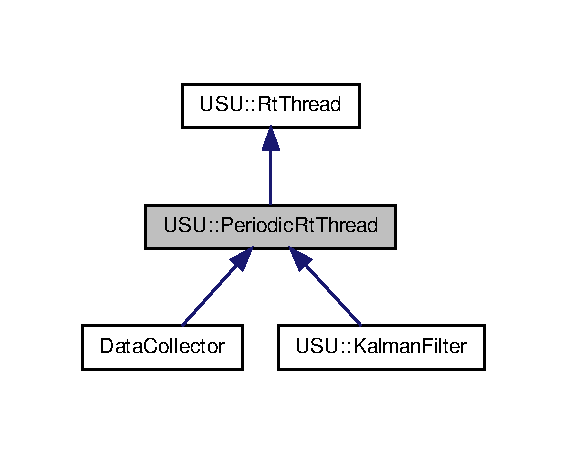
\includegraphics[width=350pt]{class_u_s_u_1_1_periodic_rt_thread__inherit__graph}
\end{center}
\end{figure}


\-Collaboration diagram for \-U\-S\-U\-:\-:\-Periodic\-Rt\-Thread\-:\nopagebreak
\begin{figure}[H]
\begin{center}
\leavevmode
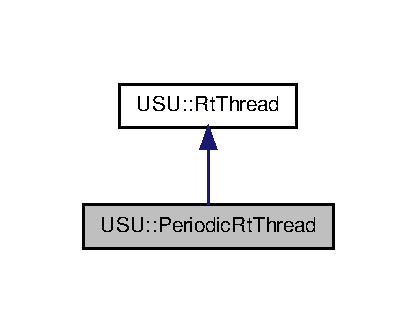
\includegraphics[width=200pt]{class_u_s_u_1_1_periodic_rt_thread__coll__graph}
\end{center}
\end{figure}
\subsection*{\-Public \-Member \-Functions}
\begin{DoxyCompactItemize}
\item 
\hyperlink{class_u_s_u_1_1_periodic_rt_thread_a1106f9ea06df9739369c5994be340624}{\-Periodic\-Rt\-Thread} (int priority=0, unsigned int period\-\_\-us=1000000)
\begin{DoxyCompactList}\small\item\em \-Creates the \hyperlink{class_u_s_u_1_1_periodic_rt_thread}{\-Periodic\-Rt\-Thread} object. \end{DoxyCompactList}\item 
virtual void \hyperlink{class_u_s_u_1_1_periodic_rt_thread_ac9146b3088a9b268594ce41d002d020a}{run} ()=0
\begin{DoxyCompactList}\small\item\em \-Actual method of the thread is running. \end{DoxyCompactList}\end{DoxyCompactItemize}
\subsection*{\-Protected \-Member \-Functions}
\begin{DoxyCompactItemize}
\item 
void \hyperlink{class_u_s_u_1_1_periodic_rt_thread_a99fd532b61ad6fd0481b842343c8e954}{make\-Thread\-Periodic} ()
\begin{DoxyCompactList}\small\item\em \-Registers the \-Periodic timer. \end{DoxyCompactList}\item 
void \hyperlink{class_u_s_u_1_1_periodic_rt_thread_a4664082b226e48204cb35fc7715b82fd}{wait\-Period} ()
\begin{DoxyCompactList}\small\item\em \-Blocks the thread until the next timer event. \end{DoxyCompactList}\end{DoxyCompactItemize}


\subsection{\-Detailed \-Description}
\-T\-O\-D\-O\-: \-Make some proper exceptions. 

\-Abstract wrapper class for a periodic thread usign the pthread library with \-R\-T-\/priority

\-Based on \hyperlink{class_u_s_u_1_1_rt_thread}{\-Rt\-Thread} this class uses pthread underneath but creates a periodic timer event it can wait for in a (forever) loop. \-This is more accurate than the use of nanosleep as the execution time of the loop will not be taken into account. \-It is therefore designed for periodic work where high accuracy is desired. 

\-Definition at line 30 of file periodicrtthread.\-h.



\subsection{\-Constructor \& \-Destructor \-Documentation}
\hypertarget{class_u_s_u_1_1_periodic_rt_thread_a1106f9ea06df9739369c5994be340624}{\index{\-U\-S\-U\-::\-Periodic\-Rt\-Thread@{\-U\-S\-U\-::\-Periodic\-Rt\-Thread}!\-Periodic\-Rt\-Thread@{\-Periodic\-Rt\-Thread}}
\index{\-Periodic\-Rt\-Thread@{\-Periodic\-Rt\-Thread}!USU::PeriodicRtThread@{\-U\-S\-U\-::\-Periodic\-Rt\-Thread}}
\subsubsection[{\-Periodic\-Rt\-Thread}]{\setlength{\rightskip}{0pt plus 5cm}\-Periodic\-Rt\-Thread\-::\-Periodic\-Rt\-Thread (
\begin{DoxyParamCaption}
\item[{int}]{priority = {\ttfamily 0}, }
\item[{unsigned int}]{period\-\_\-us = {\ttfamily 1000000}}
\end{DoxyParamCaption}
)}}\label{class_u_s_u_1_1_periodic_rt_thread_a1106f9ea06df9739369c5994be340624}


\-Creates the \hyperlink{class_u_s_u_1_1_periodic_rt_thread}{\-Periodic\-Rt\-Thread} object. 

\-Calls the constructor of the parent \hyperlink{class_u_s_u_1_1_rt_thread}{\-Rt\-Thread} and registers the periodic timer


\begin{DoxyParams}{\-Parameters}
{\em priority} & the \-Priority of the \-Thread (\-Linux\-: 1..99) \\
\hline
{\em period\-\_\-us} & \-Period of the thread in us \\
\hline
\end{DoxyParams}


\-Definition at line 22 of file periodicrtthread.\-cpp.



\subsection{\-Member \-Function \-Documentation}
\hypertarget{class_u_s_u_1_1_periodic_rt_thread_a99fd532b61ad6fd0481b842343c8e954}{\index{\-U\-S\-U\-::\-Periodic\-Rt\-Thread@{\-U\-S\-U\-::\-Periodic\-Rt\-Thread}!make\-Thread\-Periodic@{make\-Thread\-Periodic}}
\index{make\-Thread\-Periodic@{make\-Thread\-Periodic}!USU::PeriodicRtThread@{\-U\-S\-U\-::\-Periodic\-Rt\-Thread}}
\subsubsection[{make\-Thread\-Periodic}]{\setlength{\rightskip}{0pt plus 5cm}void {\bf \-Periodic\-Rt\-Thread\-::make\-Thread\-Periodic} (
\begin{DoxyParamCaption}
{}
\end{DoxyParamCaption}
)\hspace{0.3cm}{\ttfamily  \mbox{[}protected\mbox{]}}}}\label{class_u_s_u_1_1_periodic_rt_thread_a99fd532b61ad6fd0481b842343c8e954}


\-Registers the \-Periodic timer. 

\-T\-O\-D\-O\-: create exception 

\-Definition at line 29 of file periodicrtthread.\-cpp.

\hypertarget{class_u_s_u_1_1_periodic_rt_thread_ac9146b3088a9b268594ce41d002d020a}{\index{\-U\-S\-U\-::\-Periodic\-Rt\-Thread@{\-U\-S\-U\-::\-Periodic\-Rt\-Thread}!run@{run}}
\index{run@{run}!USU::PeriodicRtThread@{\-U\-S\-U\-::\-Periodic\-Rt\-Thread}}
\subsubsection[{run}]{\setlength{\rightskip}{0pt plus 5cm}virtual void {\bf \-U\-S\-U\-::\-Periodic\-Rt\-Thread\-::run} (
\begin{DoxyParamCaption}
{}
\end{DoxyParamCaption}
)\hspace{0.3cm}{\ttfamily  \mbox{[}pure virtual\mbox{]}}}}\label{class_u_s_u_1_1_periodic_rt_thread_ac9146b3088a9b268594ce41d002d020a}


\-Actual method of the thread is running. 

\-Every child class has to implement this function in order to do some threaded work. 

\-Implements \hyperlink{class_u_s_u_1_1_rt_thread_a858a5d475ed5b61759889b6608ff4372}{\-U\-S\-U\-::\-Rt\-Thread}.



\-Implemented in \hyperlink{class_my_thread_a48f2e366e852087c53705f64e1ee65c2}{\-My\-Thread}, \hyperlink{class_u_s_u_1_1_kalman_filter_a47cc7f620b57b25133289e61dbf2a7be}{\-U\-S\-U\-::\-Kalman\-Filter}, and \hyperlink{class_data_collector_acb6910eac48d5992e2bd9c43cfcd8ca5}{\-Data\-Collector}.

\hypertarget{class_u_s_u_1_1_periodic_rt_thread_a4664082b226e48204cb35fc7715b82fd}{\index{\-U\-S\-U\-::\-Periodic\-Rt\-Thread@{\-U\-S\-U\-::\-Periodic\-Rt\-Thread}!wait\-Period@{wait\-Period}}
\index{wait\-Period@{wait\-Period}!USU::PeriodicRtThread@{\-U\-S\-U\-::\-Periodic\-Rt\-Thread}}
\subsubsection[{wait\-Period}]{\setlength{\rightskip}{0pt plus 5cm}void {\bf \-Periodic\-Rt\-Thread\-::wait\-Period} (
\begin{DoxyParamCaption}
{}
\end{DoxyParamCaption}
)\hspace{0.3cm}{\ttfamily  \mbox{[}protected\mbox{]}}}}\label{class_u_s_u_1_1_periodic_rt_thread_a4664082b226e48204cb35fc7715b82fd}


\-Blocks the thread until the next timer event. 

\-Waits the remaining time until the next timer event happens. \-Thus wait\-Time = m\-Period\-\_\-us -\/ runtime since last timer event 

\-Definition at line 56 of file periodicrtthread.\-cpp.



\-The documentation for this class was generated from the following files\-:\begin{DoxyCompactItemize}
\item 
include/\hyperlink{periodicrtthread_8h}{periodicrtthread.\-h}\item 
src/\hyperlink{periodicrtthread_8cpp}{periodicrtthread.\-cpp}\end{DoxyCompactItemize}

\input{class_u_s_u_1_1_raw_acc_ang}
\hypertarget{class_u_s_u_1_1_rt_thread}{\section{\-U\-S\-U\-:\-:\-Rt\-Thread \-Class \-Reference}
\label{class_u_s_u_1_1_rt_thread}\index{\-U\-S\-U\-::\-Rt\-Thread@{\-U\-S\-U\-::\-Rt\-Thread}}
}


\-Abstract wrapper class for the pthread library with \-R\-T-\/priority.  




{\ttfamily \#include $<$\-Rt\-Thread.\-h$>$}



\-Inheritance diagram for \-U\-S\-U\-:\-:\-Rt\-Thread\-:
\nopagebreak
\begin{figure}[H]
\begin{center}
\leavevmode
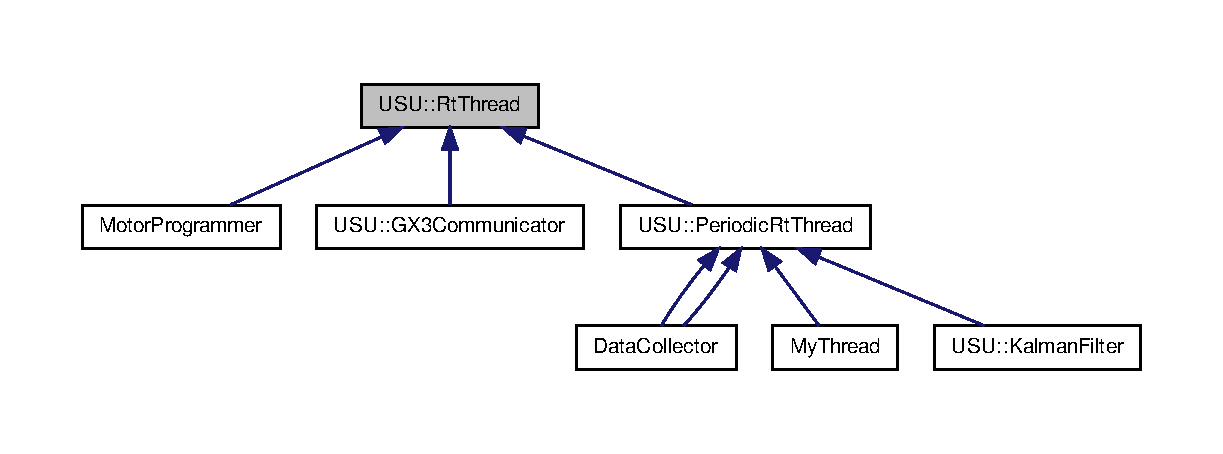
\includegraphics[width=350pt]{class_u_s_u_1_1_rt_thread__inherit__graph}
\end{center}
\end{figure}
\subsection*{\-Public \-Member \-Functions}
\begin{DoxyCompactItemize}
\item 
\hyperlink{class_u_s_u_1_1_rt_thread_a9b72ca126bc7f53871ec78635540e037}{\-Rt\-Thread} (int priority=0)
\begin{DoxyCompactList}\small\item\em \-Creates the \hyperlink{class_u_s_u_1_1_rt_thread}{\-Rt\-Thread} object. \end{DoxyCompactList}\item 
virtual \hyperlink{class_u_s_u_1_1_rt_thread_ab1ec23dd67ba0d1ad0193416a1ed8243}{$\sim$\-Rt\-Thread} ()
\begin{DoxyCompactList}\small\item\em \-Destructor of the \hyperlink{class_u_s_u_1_1_rt_thread}{\-Rt\-Thread} object. \end{DoxyCompactList}\item 
pthread\-\_\-t \hyperlink{class_u_s_u_1_1_rt_thread_a8432c713bb9f0fca217d822970b3ec54}{get\-Thread\-Id} () const 
\begin{DoxyCompactList}\small\item\em \-Return the pthread handle. \end{DoxyCompactList}\item 
int \hyperlink{class_u_s_u_1_1_rt_thread_ac26891d04e6b5fc487d5325ca0c90ead}{get\-Priority} () const 
\begin{DoxyCompactList}\small\item\em \-Returns the priority of the thread. \end{DoxyCompactList}\item 
void \hyperlink{class_u_s_u_1_1_rt_thread_aadd18e02db9c71911671936247d0ac70}{start} (void $\ast$args=\-N\-U\-L\-L)
\begin{DoxyCompactList}\small\item\em \-Creates and starts the pthread. \end{DoxyCompactList}\item 
void \hyperlink{class_u_s_u_1_1_rt_thread_ae9ee3caaab9d46341c779ff67b27926d}{join} ()
\begin{DoxyCompactList}\small\item\em \-Waits for the thread to join. \end{DoxyCompactList}\item 
virtual void \hyperlink{class_u_s_u_1_1_rt_thread_a858a5d475ed5b61759889b6608ff4372}{run} ()=0
\begin{DoxyCompactList}\small\item\em \-Actual method of the thread is running. \end{DoxyCompactList}\end{DoxyCompactItemize}
\subsection*{\-Static \-Protected \-Member \-Functions}
\begin{DoxyCompactItemize}
\item 
static void $\ast$ \hyperlink{class_u_s_u_1_1_rt_thread_ab971fca9b0e83f4101ca9c1723af4bdc}{exec} (void $\ast$thr)
\begin{DoxyCompactList}\small\item\em \-Function passed to pthread\-\_\-create, do not call manually! \end{DoxyCompactList}\end{DoxyCompactItemize}
\subsection*{\-Protected \-Attributes}
\begin{DoxyCompactItemize}
\item 
pthread\-\_\-t \hyperlink{class_u_s_u_1_1_rt_thread_afe45711f791a727426c6b0e23add03a8}{m\-Id}
\item 
bool \hyperlink{class_u_s_u_1_1_rt_thread_a990cc76b2f9541a6dbafdfa6be5fd367}{m\-Started}
\item 
void $\ast$ \hyperlink{class_u_s_u_1_1_rt_thread_a5213699b8def7e9e2af0add4648b8b40}{m\-Args}
\end{DoxyCompactItemize}


\subsection{\-Detailed \-Description}
\-Abstract wrapper class for the pthread library with \-R\-T-\/priority. 

\-This class is a thin wrapper for the pthread library. \-Inherited classes need to implement the run function with the tasks for the thread. \-The thread will run with the \-S\-C\-H\-E\-D\-\_\-\-F\-I\-F\-O-\/scheduler at the set priority. \-Therefore root rights are necessary for changing the scheduling policy. 

\-Definition at line 29 of file \-Rt\-Thread.\-h.



\subsection{\-Constructor \& \-Destructor \-Documentation}
\hypertarget{class_u_s_u_1_1_rt_thread_a9b72ca126bc7f53871ec78635540e037}{\index{\-U\-S\-U\-::\-Rt\-Thread@{\-U\-S\-U\-::\-Rt\-Thread}!\-Rt\-Thread@{\-Rt\-Thread}}
\index{\-Rt\-Thread@{\-Rt\-Thread}!USU::RtThread@{\-U\-S\-U\-::\-Rt\-Thread}}
\subsubsection[{\-Rt\-Thread}]{\setlength{\rightskip}{0pt plus 5cm}\-Rt\-Thread\-::\-Rt\-Thread (
\begin{DoxyParamCaption}
\item[{int}]{priority = {\ttfamily 0}}
\end{DoxyParamCaption}
)}}\label{class_u_s_u_1_1_rt_thread_a9b72ca126bc7f53871ec78635540e037}


\-Creates the \hyperlink{class_u_s_u_1_1_rt_thread}{\-Rt\-Thread} object. 

\-Prepares the \-Attribute object which is passed to pthread\-\_\-create later.


\begin{DoxyParams}{\-Parameters}
{\em priority} & the \-Priority of the \-Thread (\-Linux\-: 1..99) \\
\hline
\end{DoxyParams}


\-Definition at line 17 of file \-Rt\-Thread.\-cpp.

\hypertarget{class_u_s_u_1_1_rt_thread_ab1ec23dd67ba0d1ad0193416a1ed8243}{\index{\-U\-S\-U\-::\-Rt\-Thread@{\-U\-S\-U\-::\-Rt\-Thread}!$\sim$\-Rt\-Thread@{$\sim$\-Rt\-Thread}}
\index{$\sim$\-Rt\-Thread@{$\sim$\-Rt\-Thread}!USU::RtThread@{\-U\-S\-U\-::\-Rt\-Thread}}
\subsubsection[{$\sim$\-Rt\-Thread}]{\setlength{\rightskip}{0pt plus 5cm}{\bf \-Rt\-Thread\-::$\sim$\-Rt\-Thread} (
\begin{DoxyParamCaption}
{}
\end{DoxyParamCaption}
)\hspace{0.3cm}{\ttfamily  \mbox{[}virtual\mbox{]}}}}\label{class_u_s_u_1_1_rt_thread_ab1ec23dd67ba0d1ad0193416a1ed8243}


\-Destructor of the \hyperlink{class_u_s_u_1_1_rt_thread}{\-Rt\-Thread} object. 

\-Waits for the thread to join (if not already) and releases the \-Attributes object. 

\-Definition at line 60 of file \-Rt\-Thread.\-cpp.



\subsection{\-Member \-Function \-Documentation}
\hypertarget{class_u_s_u_1_1_rt_thread_ab971fca9b0e83f4101ca9c1723af4bdc}{\index{\-U\-S\-U\-::\-Rt\-Thread@{\-U\-S\-U\-::\-Rt\-Thread}!exec@{exec}}
\index{exec@{exec}!USU::RtThread@{\-U\-S\-U\-::\-Rt\-Thread}}
\subsubsection[{exec}]{\setlength{\rightskip}{0pt plus 5cm}void $\ast$ {\bf \-Rt\-Thread\-::exec} (
\begin{DoxyParamCaption}
\item[{void $\ast$}]{thr}
\end{DoxyParamCaption}
)\hspace{0.3cm}{\ttfamily  \mbox{[}static, protected\mbox{]}}}}\label{class_u_s_u_1_1_rt_thread_ab971fca9b0e83f4101ca9c1723af4bdc}


\-Function passed to pthread\-\_\-create, do not call manually! 

\-This function builds the interface to the pthread library. \-Only purpose is to be compatible to pthread\-\_\-create, as it will immediately call run of this class.


\begin{DoxyParams}{\-Parameters}
{\em thr} & pointer to this instance of the class. \\
\hline
\end{DoxyParams}


\-Definition at line 118 of file \-Rt\-Thread.\-cpp.

\hypertarget{class_u_s_u_1_1_rt_thread_ac26891d04e6b5fc487d5325ca0c90ead}{\index{\-U\-S\-U\-::\-Rt\-Thread@{\-U\-S\-U\-::\-Rt\-Thread}!get\-Priority@{get\-Priority}}
\index{get\-Priority@{get\-Priority}!USU::RtThread@{\-U\-S\-U\-::\-Rt\-Thread}}
\subsubsection[{get\-Priority}]{\setlength{\rightskip}{0pt plus 5cm}int {\bf \-Rt\-Thread\-::get\-Priority} (
\begin{DoxyParamCaption}
{}
\end{DoxyParamCaption}
) const\hspace{0.3cm}{\ttfamily  \mbox{[}inline\mbox{]}}}}\label{class_u_s_u_1_1_rt_thread_ac26891d04e6b5fc487d5325ca0c90ead}


\-Returns the priority of the thread. 

\begin{DoxyReturn}{\-Returns}
int priority 
\end{DoxyReturn}


\-Definition at line 82 of file \-Rt\-Thread.\-cpp.

\hypertarget{class_u_s_u_1_1_rt_thread_a8432c713bb9f0fca217d822970b3ec54}{\index{\-U\-S\-U\-::\-Rt\-Thread@{\-U\-S\-U\-::\-Rt\-Thread}!get\-Thread\-Id@{get\-Thread\-Id}}
\index{get\-Thread\-Id@{get\-Thread\-Id}!USU::RtThread@{\-U\-S\-U\-::\-Rt\-Thread}}
\subsubsection[{get\-Thread\-Id}]{\setlength{\rightskip}{0pt plus 5cm}pthread\-\_\-t {\bf \-Rt\-Thread\-::get\-Thread\-Id} (
\begin{DoxyParamCaption}
{}
\end{DoxyParamCaption}
) const\hspace{0.3cm}{\ttfamily  \mbox{[}inline\mbox{]}}}}\label{class_u_s_u_1_1_rt_thread_a8432c713bb9f0fca217d822970b3ec54}


\-Return the pthread handle. 

\begin{DoxyReturn}{\-Returns}
pthread\-\_\-t the thread handle of the last started pthread or -\/1 (if no pthread was started) 
\end{DoxyReturn}


\-Definition at line 76 of file \-Rt\-Thread.\-cpp.

\hypertarget{class_u_s_u_1_1_rt_thread_ae9ee3caaab9d46341c779ff67b27926d}{\index{\-U\-S\-U\-::\-Rt\-Thread@{\-U\-S\-U\-::\-Rt\-Thread}!join@{join}}
\index{join@{join}!USU::RtThread@{\-U\-S\-U\-::\-Rt\-Thread}}
\subsubsection[{join}]{\setlength{\rightskip}{0pt plus 5cm}void {\bf \-Rt\-Thread\-::join} (
\begin{DoxyParamCaption}
{}
\end{DoxyParamCaption}
)}}\label{class_u_s_u_1_1_rt_thread_ae9ee3caaab9d46341c779ff67b27926d}


\-Waits for the thread to join. 



\-Definition at line 108 of file \-Rt\-Thread.\-cpp.

\hypertarget{class_u_s_u_1_1_rt_thread_a858a5d475ed5b61759889b6608ff4372}{\index{\-U\-S\-U\-::\-Rt\-Thread@{\-U\-S\-U\-::\-Rt\-Thread}!run@{run}}
\index{run@{run}!USU::RtThread@{\-U\-S\-U\-::\-Rt\-Thread}}
\subsubsection[{run}]{\setlength{\rightskip}{0pt plus 5cm}virtual void {\bf \-U\-S\-U\-::\-Rt\-Thread\-::run} (
\begin{DoxyParamCaption}
{}
\end{DoxyParamCaption}
)\hspace{0.3cm}{\ttfamily  \mbox{[}pure virtual\mbox{]}}}}\label{class_u_s_u_1_1_rt_thread_a858a5d475ed5b61759889b6608ff4372}


\-Actual method of the thread is running. 

\-Every child class has to implement this function in order to do some threaded work. 

\-Implemented in \hyperlink{class_u_s_u_1_1_periodic_rt_thread_ac9146b3088a9b268594ce41d002d020a}{\-U\-S\-U\-::\-Periodic\-Rt\-Thread}, \hyperlink{class_u_s_u_1_1_motor_control_a1c7a621170352b9bdd4e5a60feee24c8}{\-U\-S\-U\-::\-Motor\-Control}, \hyperlink{class_u_s_u_1_1_kalman_filter_a47cc7f620b57b25133289e61dbf2a7be}{\-U\-S\-U\-::\-Kalman\-Filter}, and \hyperlink{class_u_s_u_1_1_g_x3_communicator_ae7e5cf4c792ca270826dea243abbc5aa}{\-U\-S\-U\-::\-G\-X3\-Communicator}.

\hypertarget{class_u_s_u_1_1_rt_thread_aadd18e02db9c71911671936247d0ac70}{\index{\-U\-S\-U\-::\-Rt\-Thread@{\-U\-S\-U\-::\-Rt\-Thread}!start@{start}}
\index{start@{start}!USU::RtThread@{\-U\-S\-U\-::\-Rt\-Thread}}
\subsubsection[{start}]{\setlength{\rightskip}{0pt plus 5cm}void {\bf \-Rt\-Thread\-::start} (
\begin{DoxyParamCaption}
\item[{void $\ast$}]{args = {\ttfamily \-N\-U\-L\-L}}
\end{DoxyParamCaption}
)}}\label{class_u_s_u_1_1_rt_thread_aadd18e02db9c71911671936247d0ac70}


\-Creates and starts the pthread. 

\-Creates the pthread with the desired attributes.


\begin{DoxyParams}{\-Parameters}
{\em args} & optional arguments for the thread \\
\hline
\end{DoxyParams}


\-Definition at line 87 of file \-Rt\-Thread.\-cpp.



\subsection{\-Member \-Data \-Documentation}
\hypertarget{class_u_s_u_1_1_rt_thread_a5213699b8def7e9e2af0add4648b8b40}{\index{\-U\-S\-U\-::\-Rt\-Thread@{\-U\-S\-U\-::\-Rt\-Thread}!m\-Args@{m\-Args}}
\index{m\-Args@{m\-Args}!USU::RtThread@{\-U\-S\-U\-::\-Rt\-Thread}}
\subsubsection[{m\-Args}]{\setlength{\rightskip}{0pt plus 5cm}void$\ast$ {\bf \-U\-S\-U\-::\-Rt\-Thread\-::m\-Args}\hspace{0.3cm}{\ttfamily  \mbox{[}protected\mbox{]}}}}\label{class_u_s_u_1_1_rt_thread_a5213699b8def7e9e2af0add4648b8b40}
\-Arguments which can be passed to a certain thread thread 

\-Definition at line 42 of file \-Rt\-Thread.\-h.

\hypertarget{class_u_s_u_1_1_rt_thread_afe45711f791a727426c6b0e23add03a8}{\index{\-U\-S\-U\-::\-Rt\-Thread@{\-U\-S\-U\-::\-Rt\-Thread}!m\-Id@{m\-Id}}
\index{m\-Id@{m\-Id}!USU::RtThread@{\-U\-S\-U\-::\-Rt\-Thread}}
\subsubsection[{m\-Id}]{\setlength{\rightskip}{0pt plus 5cm}pthread\-\_\-t {\bf \-U\-S\-U\-::\-Rt\-Thread\-::m\-Id}\hspace{0.3cm}{\ttfamily  \mbox{[}protected\mbox{]}}}}\label{class_u_s_u_1_1_rt_thread_afe45711f791a727426c6b0e23add03a8}
\-The thread handle 

\-Definition at line 40 of file \-Rt\-Thread.\-h.

\hypertarget{class_u_s_u_1_1_rt_thread_a990cc76b2f9541a6dbafdfa6be5fd367}{\index{\-U\-S\-U\-::\-Rt\-Thread@{\-U\-S\-U\-::\-Rt\-Thread}!m\-Started@{m\-Started}}
\index{m\-Started@{m\-Started}!USU::RtThread@{\-U\-S\-U\-::\-Rt\-Thread}}
\subsubsection[{m\-Started}]{\setlength{\rightskip}{0pt plus 5cm}bool {\bf \-U\-S\-U\-::\-Rt\-Thread\-::m\-Started}\hspace{0.3cm}{\ttfamily  \mbox{[}protected\mbox{]}}}}\label{class_u_s_u_1_1_rt_thread_a990cc76b2f9541a6dbafdfa6be5fd367}
\-Keeps the status of the thread \-T\-O\-D\-O\-: \-Useful?? 

\-Definition at line 41 of file \-Rt\-Thread.\-h.



\-The documentation for this class was generated from the following files\-:\begin{DoxyCompactItemize}
\item 
threading/\hyperlink{_rt_thread_8h}{\-Rt\-Thread.\-h}\item 
threading/\hyperlink{_rt_thread_8cpp}{\-Rt\-Thread.\-cpp}\end{DoxyCompactItemize}

\input{class_u_s_u_1_1_sampling_settings}
\hypertarget{class_u_s_u_1_1_scoped_lock}{\subsection{\-U\-S\-U\-:\-:\-Scoped\-Lock \-Class \-Reference}
\label{class_u_s_u_1_1_scoped_lock}\index{\-U\-S\-U\-::\-Scoped\-Lock@{\-U\-S\-U\-::\-Scoped\-Lock}}
}


\-Provides a helper class for \-Scoped \-Mutexes.  




{\ttfamily \#include $<$\-Lock.\-h$>$}

\subsubsection*{\-Public \-Member \-Functions}
\begin{DoxyCompactItemize}
\item 
\hyperlink{class_u_s_u_1_1_scoped_lock_aa92db605fefa48f75be29b86ad0d6186}{\-Scoped\-Lock} (\hyperlink{class_u_s_u_1_1_lock}{\-Lock} \&lock)
\begin{DoxyCompactList}\small\item\em \-Constructor\-: will lock the mutex. \end{DoxyCompactList}\item 
virtual \hyperlink{class_u_s_u_1_1_scoped_lock_a5cf581cbe18004e6fec30724c5f94071}{$\sim$\-Scoped\-Lock} ()
\begin{DoxyCompactList}\small\item\em \-Destructor\-: will unlock the mutex. \end{DoxyCompactList}\end{DoxyCompactItemize}


\subsubsection{\-Detailed \-Description}
\-Provides a helper class for \-Scoped \-Mutexes. 

\-Create this object by passing a reference to a \hyperlink{class_u_s_u_1_1_lock}{\-Lock} object. \-It will lock the mutex when created and unlock it when destroyed, i.\-e. when going out of scope at the end of the \char`\"{}\}\char`\"{}. \-Can make it more convenient than manual (un)locking.

\-T\-O\-D\-O\-: \-Test if it works correctly with a getter-\/method 

\-Definition at line \hyperlink{_lock_8h_source_l00092}{92} of file \hyperlink{_lock_8h_source}{\-Lock.\-h}.



\subsubsection{\-Constructor \& \-Destructor \-Documentation}
\hypertarget{class_u_s_u_1_1_scoped_lock_aa92db605fefa48f75be29b86ad0d6186}{\index{\-U\-S\-U\-::\-Scoped\-Lock@{\-U\-S\-U\-::\-Scoped\-Lock}!\-Scoped\-Lock@{\-Scoped\-Lock}}
\index{\-Scoped\-Lock@{\-Scoped\-Lock}!USU::ScopedLock@{\-U\-S\-U\-::\-Scoped\-Lock}}
\paragraph[{\-Scoped\-Lock}]{\setlength{\rightskip}{0pt plus 5cm}\-U\-S\-U\-::\-Scoped\-Lock\-::\-Scoped\-Lock (
\begin{DoxyParamCaption}
\item[{{\bf \-Lock} \&}]{lock}
\end{DoxyParamCaption}
)\hspace{0.3cm}{\ttfamily  \mbox{[}inline\mbox{]}}}}\label{class_u_s_u_1_1_scoped_lock_aa92db605fefa48f75be29b86ad0d6186}


\-Constructor\-: will lock the mutex. 


\begin{DoxyParams}{\-Parameters}
{\em lock} & \-Reference to the \hyperlink{class_u_s_u_1_1_lock}{\-Lock} it needs to hold \\
\hline
\end{DoxyParams}


\-Definition at line \hyperlink{_lock_8h_source_l00115}{115} of file \hyperlink{_lock_8h_source}{\-Lock.\-h}.

\hypertarget{class_u_s_u_1_1_scoped_lock_a5cf581cbe18004e6fec30724c5f94071}{\index{\-U\-S\-U\-::\-Scoped\-Lock@{\-U\-S\-U\-::\-Scoped\-Lock}!$\sim$\-Scoped\-Lock@{$\sim$\-Scoped\-Lock}}
\index{$\sim$\-Scoped\-Lock@{$\sim$\-Scoped\-Lock}!USU::ScopedLock@{\-U\-S\-U\-::\-Scoped\-Lock}}
\paragraph[{$\sim$\-Scoped\-Lock}]{\setlength{\rightskip}{0pt plus 5cm}{\bf \-U\-S\-U\-::\-Scoped\-Lock\-::$\sim$\-Scoped\-Lock} (
\begin{DoxyParamCaption}
{}
\end{DoxyParamCaption}
)\hspace{0.3cm}{\ttfamily  \mbox{[}inline, virtual\mbox{]}}}}\label{class_u_s_u_1_1_scoped_lock_a5cf581cbe18004e6fec30724c5f94071}


\-Destructor\-: will unlock the mutex. 



\-Definition at line \hyperlink{_lock_8h_source_l00122}{122} of file \hyperlink{_lock_8h_source}{\-Lock.\-h}.



\-The documentation for this class was generated from the following file\-:\begin{DoxyCompactItemize}
\item 
include/\hyperlink{_lock_8h}{\-Lock.\-h}\end{DoxyCompactItemize}

\input{class_u_s_u_1_1_set_countinuous_mode}
\chapter{\-File \-Documentation}
\input{gx3communicator_8cpp}
\input{gx3communicator_8h}
\input{messages_8h}
\input{test_8cpp}
\hypertarget{kalmanfilter_8cpp}{\section{src/kalmanfilter.cpp \-File \-Reference}
\label{kalmanfilter_8cpp}\index{src/kalmanfilter.\-cpp@{src/kalmanfilter.\-cpp}}
}
{\ttfamily \#include $<$iostream$>$}\*
{\ttfamily \#include $<$sys/time.\-h$>$}\*
{\ttfamily \#include $<$unistd.\-h$>$}\*
{\ttfamily \#include \char`\"{}kalmanfilter.\-h\char`\"{}}\*
{\ttfamily \#include \char`\"{}vector.\-h\char`\"{}}\*
\-Include dependency graph for kalmanfilter.\-cpp\-:\nopagebreak
\begin{figure}[H]
\begin{center}
\leavevmode
\includegraphics[width=350pt]{kalmanfilter_8cpp__incl}
\end{center}
\end{figure}
\subsection*{\-Functions}
\begin{DoxyCompactItemize}
\item 
int \hyperlink{kalmanfilter_8cpp_a1dec6ba085ce91733e9c4c7e6088a598}{timeval\-\_\-subtract} (struct timeval $\ast$result, struct timeval $\ast$x, struct timeval $\ast$y)
\end{DoxyCompactItemize}


\subsection{\-Detailed \-Description}
\-C++ class for the sensor fusion and stated estimated. \-Based on the \-Periodic\-Rt\-Thread class.

\begin{DoxyAuthor}{\-Author}
\-Jan \-Sommer \-Created on\-: \-Apr 20, 2013 
\end{DoxyAuthor}


\-Definition in file \hyperlink{kalmanfilter_8cpp_source}{kalmanfilter.\-cpp}.



\subsection{\-Function \-Documentation}
\hypertarget{kalmanfilter_8cpp_a1dec6ba085ce91733e9c4c7e6088a598}{\index{kalmanfilter.\-cpp@{kalmanfilter.\-cpp}!timeval\-\_\-subtract@{timeval\-\_\-subtract}}
\index{timeval\-\_\-subtract@{timeval\-\_\-subtract}!kalmanfilter.cpp@{kalmanfilter.\-cpp}}
\subsubsection[{timeval\-\_\-subtract}]{\setlength{\rightskip}{0pt plus 5cm}int {\bf timeval\-\_\-subtract} (
\begin{DoxyParamCaption}
\item[{struct timeval $\ast$}]{result, }
\item[{struct timeval $\ast$}]{x, }
\item[{struct timeval $\ast$}]{y}
\end{DoxyParamCaption}
)}}\label{kalmanfilter_8cpp_a1dec6ba085ce91733e9c4c7e6088a598}


\-Definition at line 26 of file kalmanfilter.\-cpp.


\hypertarget{kalmanfilter_8h}{\section{kalmanfilter.\-h \-File \-Reference}
\label{kalmanfilter_8h}\index{kalmanfilter.\-h@{kalmanfilter.\-h}}
}
{\ttfamily \#include \char`\"{}threading/periodicrtthread.\-h\char`\"{}}\*
{\ttfamily \#include \char`\"{}minimu/minimu.\-h\char`\"{}}\*
{\ttfamily \#include \char`\"{}threading/\-Lock.\-h\char`\"{}}\*
\-Include dependency graph for kalmanfilter.\-h\-:
\nopagebreak
\begin{figure}[H]
\begin{center}
\leavevmode

\includegraphics[width=350pt]{kalmanfilter_8h__incl}
\end{center}
\end{figure}
\-This graph shows which files directly or indirectly include this file\-:
\nopagebreak
\begin{figure}[H]
\begin{center}
\leavevmode
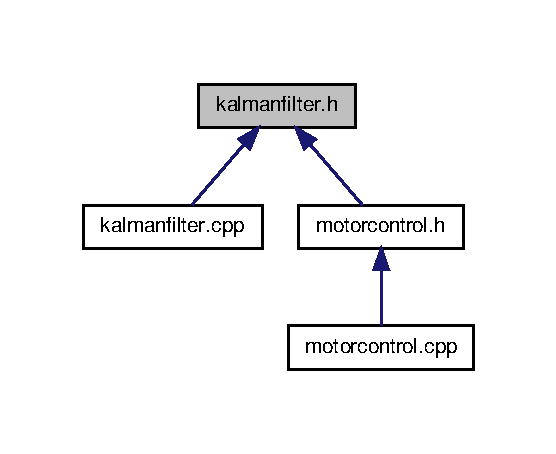
\includegraphics[width=267pt]{kalmanfilter_8h__dep__incl}
\end{center}
\end{figure}
\subsection*{\-Classes}
\begin{DoxyCompactItemize}
\item 
class \hyperlink{class_u_s_u_1_1_kalman_filter}{\-U\-S\-U\-::\-Kalman\-Filter}
\begin{DoxyCompactList}\small\item\em \-Represents the \-Periodic class for state estimation. \end{DoxyCompactList}\end{DoxyCompactItemize}
\subsection*{\-Namespaces}
\begin{DoxyCompactItemize}
\item 
namespace \hyperlink{namespace_u_s_u}{\-U\-S\-U}
\begin{DoxyCompactList}\small\item\em \-T\-O\-D\-O\-: \-Make some proper exceptions. \end{DoxyCompactList}\end{DoxyCompactItemize}


\subsection{\-Detailed \-Description}
\-C++ class for the sensor fusion and stated estimated. \-Based on the \-Periodic\-Rt\-Thread class.

\begin{DoxyAuthor}{\-Author}
\-Jan \-Sommer \-Created on\-: \-Apr 20, 2013 
\end{DoxyAuthor}


\-Definition in file \hyperlink{kalmanfilter_8h_source}{kalmanfilter.\-h}.


\hypertarget{main_8cpp}{\section{main.\-cpp \-File \-Reference}
\label{main_8cpp}\index{main.\-cpp@{main.\-cpp}}
}
{\ttfamily \#include $<$csignal$>$}\*
{\ttfamily \#include $<$cstdlib$>$}\*
{\ttfamily \#include $<$unistd.\-h$>$}\*
{\ttfamily \#include \char`\"{}kalmanfilter.\-h\char`\"{}}\*
\-Include dependency graph for main.\-cpp\-:
\nopagebreak
\begin{figure}[H]
\begin{center}
\leavevmode
\includegraphics[width=350pt]{main_8cpp__incl}
\end{center}
\end{figure}
\subsection*{\-Functions}
\begin{DoxyCompactItemize}
\item 
int \hyperlink{main_8cpp_ae66f6b31b5ad750f1fe042a706a4e3d4}{main} ()
\end{DoxyCompactItemize}
\subsection*{\-Variables}
\begin{DoxyCompactItemize}
\item 
\hyperlink{class_u_s_u_1_1_kalman_filter}{\-Kalman\-Filter} \hyperlink{main_8cpp_a0a9b6f4deb0318813fac0927f268ade3}{kalman\-Filter} (5, 20000,\char`\"{}/dev/i2c-\/2\char`\"{})
\end{DoxyCompactItemize}


\subsection{\-Function \-Documentation}
\hypertarget{main_8cpp_ae66f6b31b5ad750f1fe042a706a4e3d4}{\index{main.\-cpp@{main.\-cpp}!main@{main}}
\index{main@{main}!main.cpp@{main.\-cpp}}
\subsubsection[{main}]{\setlength{\rightskip}{0pt plus 5cm}int {\bf main} (
\begin{DoxyParamCaption}
{}
\end{DoxyParamCaption}
)}}\label{main_8cpp_ae66f6b31b5ad750f1fe042a706a4e3d4}


\-Definition at line 23 of file main.\-cpp.



\subsection{\-Variable \-Documentation}
\hypertarget{main_8cpp_a0a9b6f4deb0318813fac0927f268ade3}{\index{main.\-cpp@{main.\-cpp}!kalman\-Filter@{kalman\-Filter}}
\index{kalman\-Filter@{kalman\-Filter}!main.cpp@{main.\-cpp}}
\subsubsection[{kalman\-Filter}]{\setlength{\rightskip}{0pt plus 5cm}{\bf \-Kalman\-Filter} {\bf kalman\-Filter}(5, 20000,\char`\"{}/dev/i2c-\/2\char`\"{})}}\label{main_8cpp_a0a9b6f4deb0318813fac0927f268ade3}

\hypertarget{exceptions_8h}{\subsection{include/exceptions.h \-File \-Reference}
\label{exceptions_8h}\index{include/exceptions.\-h@{include/exceptions.\-h}}
}
{\ttfamily \#include $<$cerrno$>$}\*
{\ttfamily \#include $<$system\-\_\-error$>$}\*
\-Include dependency graph for exceptions.\-h\-:\nopagebreak
\begin{figure}[H]
\begin{center}
\leavevmode
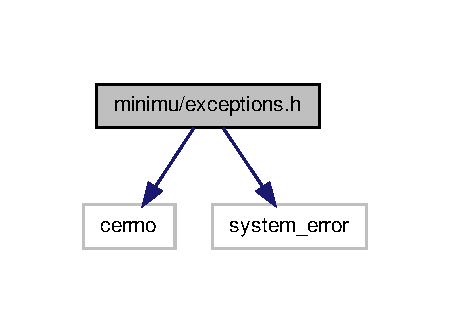
\includegraphics[width=216pt]{exceptions_8h__incl}
\end{center}
\end{figure}
\-This graph shows which files directly or indirectly include this file\-:\nopagebreak
\begin{figure}[H]
\begin{center}
\leavevmode
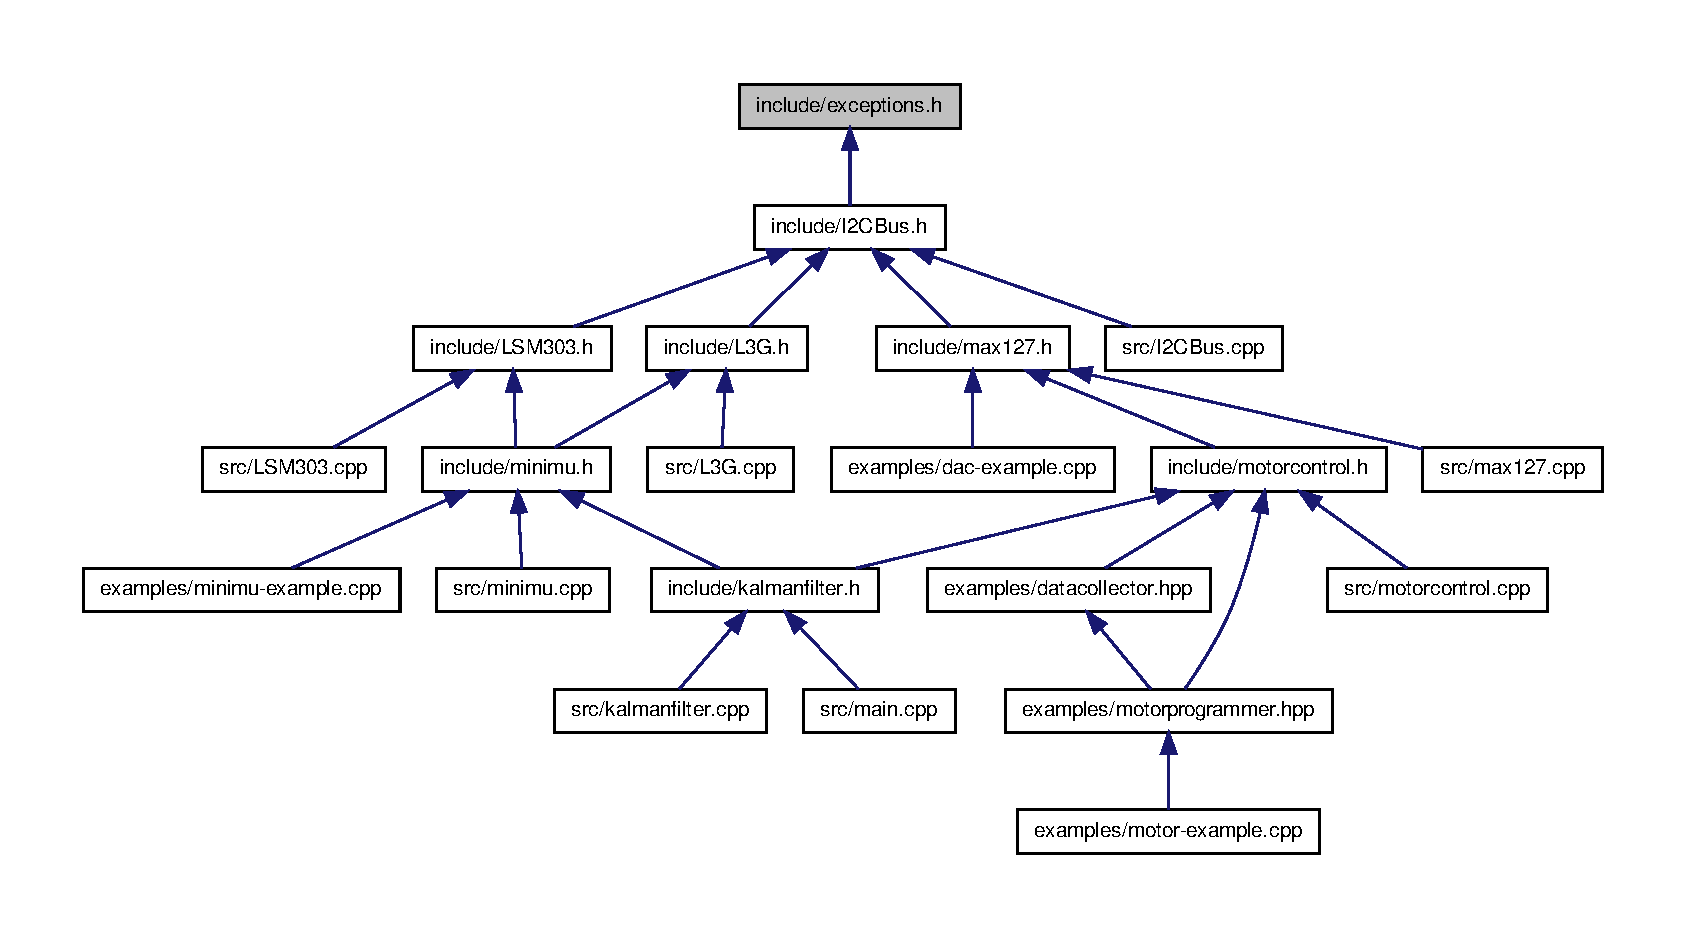
\includegraphics[width=350pt]{exceptions_8h__dep__incl}
\end{center}
\end{figure}

\hypertarget{_i2_c_bus_8cpp}{\subsection{src/\-I2\-C\-Bus.cpp \-File \-Reference}
\label{_i2_c_bus_8cpp}\index{src/\-I2\-C\-Bus.\-cpp@{src/\-I2\-C\-Bus.\-cpp}}
}
{\ttfamily \#include $<$unistd.\-h$>$}\*
{\ttfamily \#include $<$linux/i2c-\/dev.\-h$>$}\*
{\ttfamily \#include $<$fcntl.\-h$>$}\*
{\ttfamily \#include \char`\"{}\-I2\-C\-Bus.\-h\char`\"{}}\*
\-Include dependency graph for \-I2\-C\-Bus.\-cpp\-:\nopagebreak
\begin{figure}[H]
\begin{center}
\leavevmode
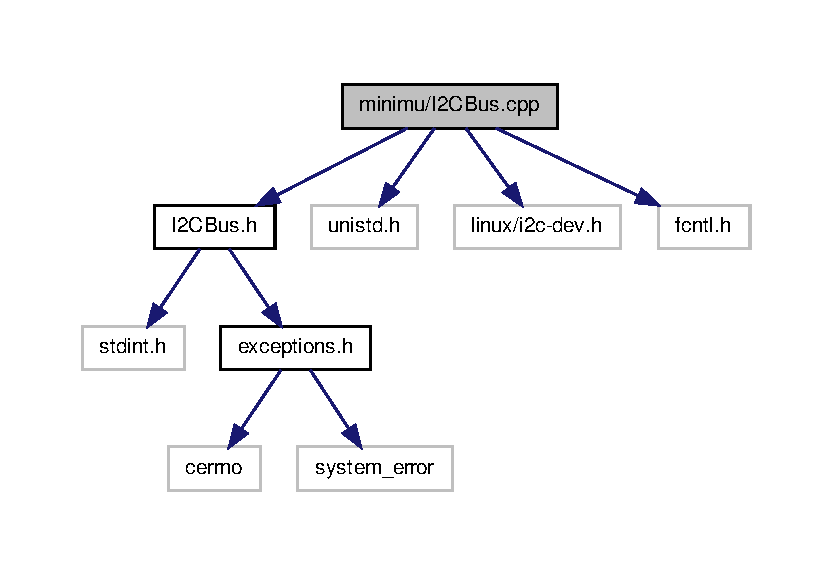
\includegraphics[width=350pt]{_i2_c_bus_8cpp__incl}
\end{center}
\end{figure}

\hypertarget{_i2_c_bus_8h}{\section{include/\-I2\-C\-Bus.h \-File \-Reference}
\label{_i2_c_bus_8h}\index{include/\-I2\-C\-Bus.\-h@{include/\-I2\-C\-Bus.\-h}}
}
{\ttfamily \#include $<$stdint.\-h$>$}\*
{\ttfamily \#include \char`\"{}exceptions.\-h\char`\"{}}\*
\-Include dependency graph for \-I2\-C\-Bus.\-h\-:\nopagebreak
\begin{figure}[H]
\begin{center}
\leavevmode
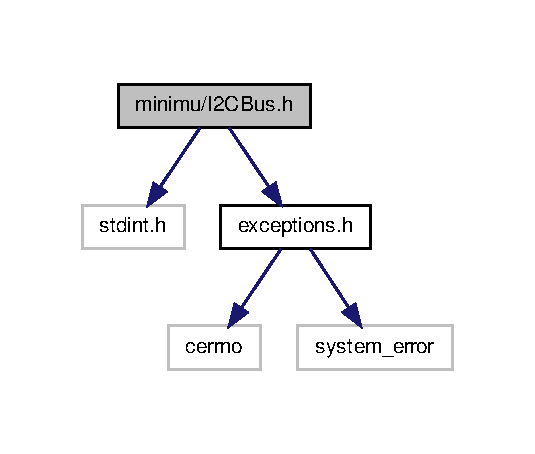
\includegraphics[width=257pt]{_i2_c_bus_8h__incl}
\end{center}
\end{figure}
\-This graph shows which files directly or indirectly include this file\-:
\nopagebreak
\begin{figure}[H]
\begin{center}
\leavevmode
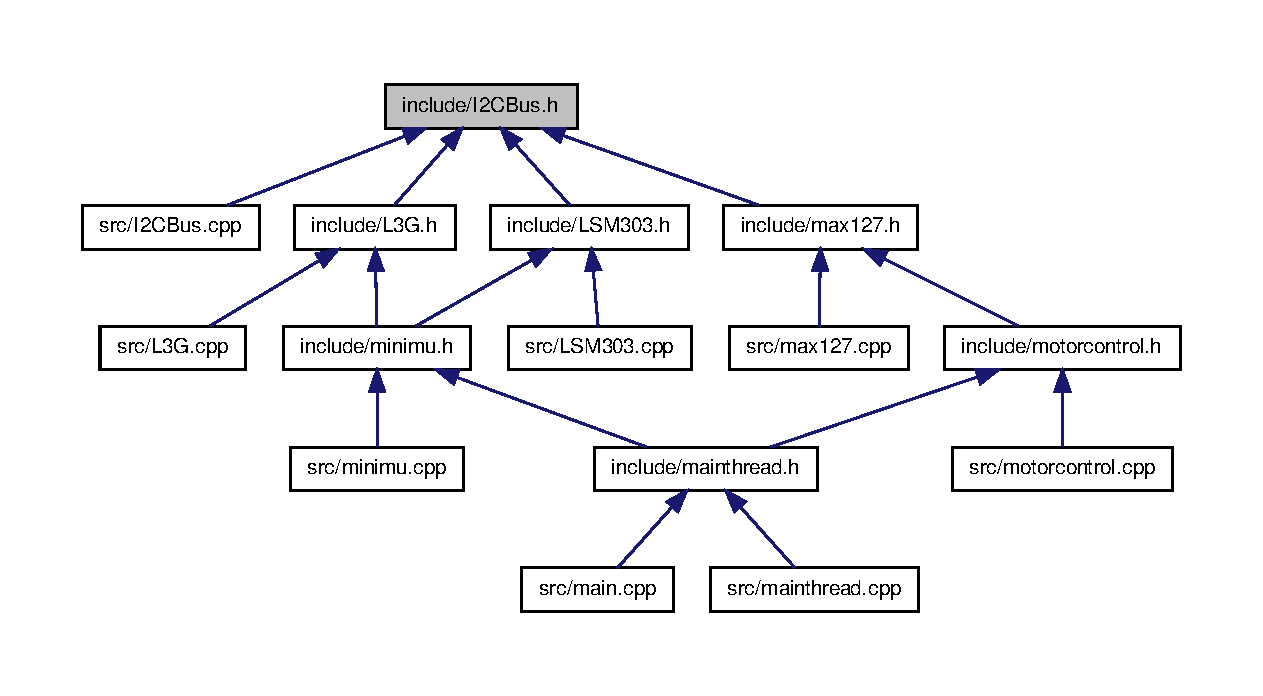
\includegraphics[width=350pt]{_i2_c_bus_8h__dep__incl}
\end{center}
\end{figure}
\subsection*{\-Classes}
\begin{DoxyCompactItemize}
\item 
class \hyperlink{class_i2_c_bus}{\-I2\-C\-Bus}
\begin{DoxyCompactList}\small\item\em \-Wrapper class for \-I2\-C-\/bus communication. \end{DoxyCompactList}\end{DoxyCompactItemize}

\hypertarget{_i_m_u_8h}{\section{include/\-I\-M\-U.h \-File \-Reference}
\label{_i_m_u_8h}\index{include/\-I\-M\-U.\-h@{include/\-I\-M\-U.\-h}}
}
{\ttfamily \#include \char`\"{}vector.\-h\char`\"{}}\*
\-Include dependency graph for \-I\-M\-U.\-h\-:\nopagebreak
\begin{figure}[H]
\begin{center}
\leavevmode
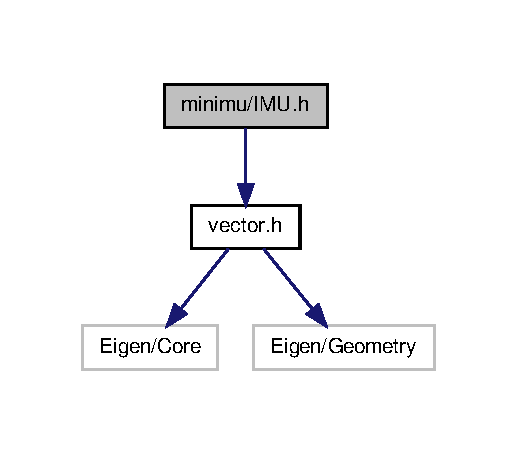
\includegraphics[width=248pt]{_i_m_u_8h__incl}
\end{center}
\end{figure}
\-This graph shows which files directly or indirectly include this file\-:\nopagebreak
\begin{figure}[H]
\begin{center}
\leavevmode
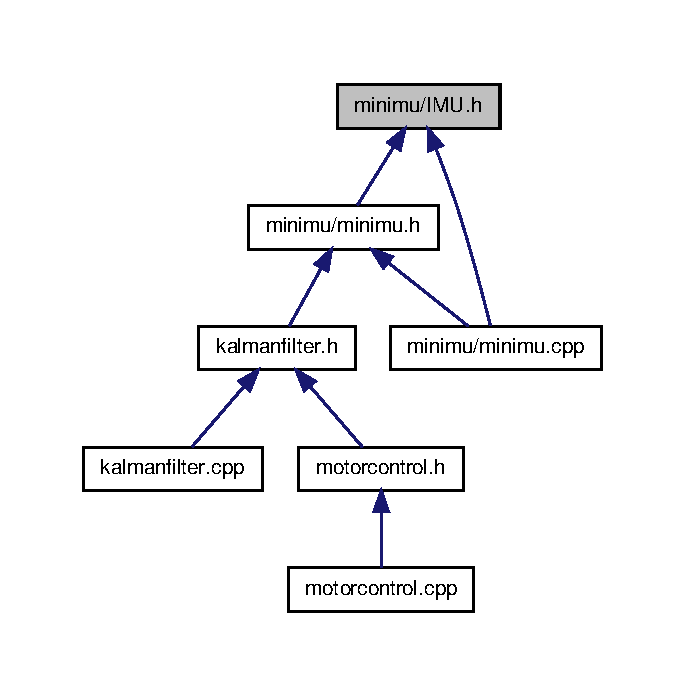
\includegraphics[width=350pt]{_i_m_u_8h__dep__incl}
\end{center}
\end{figure}
\subsection*{\-Classes}
\begin{DoxyCompactItemize}
\item 
class \hyperlink{class_i_m_u}{\-I\-M\-U}
\end{DoxyCompactItemize}

\hypertarget{_l3_g_8cpp}{\subsection{src/\-L3\-G.cpp \-File \-Reference}
\label{_l3_g_8cpp}\index{src/\-L3\-G.\-cpp@{src/\-L3\-G.\-cpp}}
}
{\ttfamily \#include $<$stdexcept$>$}\*
{\ttfamily \#include \char`\"{}\-L3\-G.\-h\char`\"{}}\*
\-Include dependency graph for \-L3\-G.\-cpp\-:\nopagebreak
\begin{figure}[H]
\begin{center}
\leavevmode
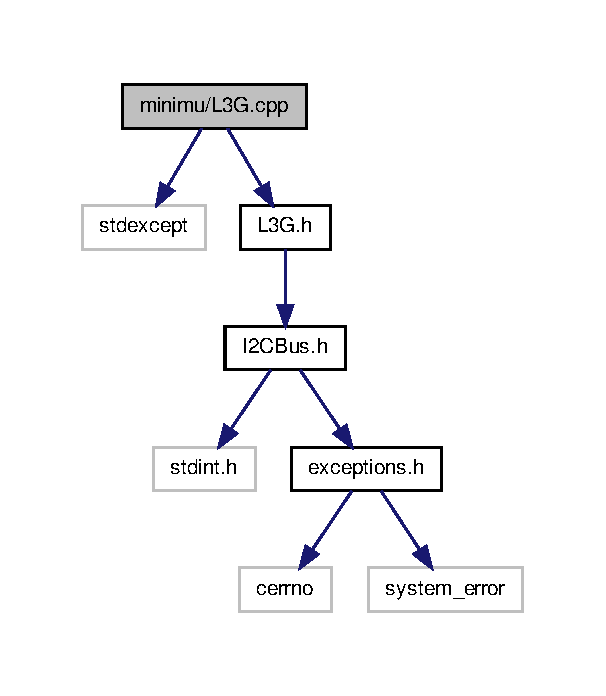
\includegraphics[width=291pt]{_l3_g_8cpp__incl}
\end{center}
\end{figure}
\subsubsection*{\-Defines}
\begin{DoxyCompactItemize}
\item 
\#define \hyperlink{_l3_g_8cpp_af6efbbfd8c5101dbb4856760f25df8ba}{\-L3\-G4200\-D\-\_\-\-A\-D\-D\-R\-E\-S\-S\-\_\-\-S\-A0\-\_\-\-L\-O\-W}~(0x\-D0 $>$$>$ 1)
\item 
\#define \hyperlink{_l3_g_8cpp_a5d64fb9cbaa290b79125b81764f7ddd0}{\-L3\-G4200\-D\-\_\-\-A\-D\-D\-R\-E\-S\-S\-\_\-\-S\-A0\-\_\-\-H\-I\-G\-H}~(0x\-D2 $>$$>$ 1)
\item 
\#define \hyperlink{_l3_g_8cpp_a49fc2c0e239dc82b4c3ce88d489004a3}{\-L3\-G\-D20\-\_\-\-A\-D\-D\-R\-E\-S\-S\-\_\-\-S\-A0\-\_\-\-L\-O\-W}~(0x\-D4 $>$$>$ 1)
\item 
\#define \hyperlink{_l3_g_8cpp_a30dbad8f4ae0051bcbc17587c6ee7703}{\-L3\-G\-D20\-\_\-\-A\-D\-D\-R\-E\-S\-S\-\_\-\-S\-A0\-\_\-\-H\-I\-G\-H}~(0x\-D6 $>$$>$ 1)
\end{DoxyCompactItemize}


\subsubsection{\-Define \-Documentation}
\hypertarget{_l3_g_8cpp_a5d64fb9cbaa290b79125b81764f7ddd0}{\index{\-L3\-G.\-cpp@{\-L3\-G.\-cpp}!\-L3\-G4200\-D\-\_\-\-A\-D\-D\-R\-E\-S\-S\-\_\-\-S\-A0\-\_\-\-H\-I\-G\-H@{\-L3\-G4200\-D\-\_\-\-A\-D\-D\-R\-E\-S\-S\-\_\-\-S\-A0\-\_\-\-H\-I\-G\-H}}
\index{\-L3\-G4200\-D\-\_\-\-A\-D\-D\-R\-E\-S\-S\-\_\-\-S\-A0\-\_\-\-H\-I\-G\-H@{\-L3\-G4200\-D\-\_\-\-A\-D\-D\-R\-E\-S\-S\-\_\-\-S\-A0\-\_\-\-H\-I\-G\-H}!L3G.cpp@{\-L3\-G.\-cpp}}
\paragraph[{\-L3\-G4200\-D\-\_\-\-A\-D\-D\-R\-E\-S\-S\-\_\-\-S\-A0\-\_\-\-H\-I\-G\-H}]{\setlength{\rightskip}{0pt plus 5cm}\#define {\bf \-L3\-G4200\-D\-\_\-\-A\-D\-D\-R\-E\-S\-S\-\_\-\-S\-A0\-\_\-\-H\-I\-G\-H}~(0x\-D2 $>$$>$ 1)}}\label{_l3_g_8cpp_a5d64fb9cbaa290b79125b81764f7ddd0}


\-Definition at line \hyperlink{_l3_g_8cpp_source_l00005}{5} of file \hyperlink{_l3_g_8cpp_source}{\-L3\-G.\-cpp}.

\hypertarget{_l3_g_8cpp_af6efbbfd8c5101dbb4856760f25df8ba}{\index{\-L3\-G.\-cpp@{\-L3\-G.\-cpp}!\-L3\-G4200\-D\-\_\-\-A\-D\-D\-R\-E\-S\-S\-\_\-\-S\-A0\-\_\-\-L\-O\-W@{\-L3\-G4200\-D\-\_\-\-A\-D\-D\-R\-E\-S\-S\-\_\-\-S\-A0\-\_\-\-L\-O\-W}}
\index{\-L3\-G4200\-D\-\_\-\-A\-D\-D\-R\-E\-S\-S\-\_\-\-S\-A0\-\_\-\-L\-O\-W@{\-L3\-G4200\-D\-\_\-\-A\-D\-D\-R\-E\-S\-S\-\_\-\-S\-A0\-\_\-\-L\-O\-W}!L3G.cpp@{\-L3\-G.\-cpp}}
\paragraph[{\-L3\-G4200\-D\-\_\-\-A\-D\-D\-R\-E\-S\-S\-\_\-\-S\-A0\-\_\-\-L\-O\-W}]{\setlength{\rightskip}{0pt plus 5cm}\#define {\bf \-L3\-G4200\-D\-\_\-\-A\-D\-D\-R\-E\-S\-S\-\_\-\-S\-A0\-\_\-\-L\-O\-W}~(0x\-D0 $>$$>$ 1)}}\label{_l3_g_8cpp_af6efbbfd8c5101dbb4856760f25df8ba}


\-Definition at line \hyperlink{_l3_g_8cpp_source_l00004}{4} of file \hyperlink{_l3_g_8cpp_source}{\-L3\-G.\-cpp}.

\hypertarget{_l3_g_8cpp_a30dbad8f4ae0051bcbc17587c6ee7703}{\index{\-L3\-G.\-cpp@{\-L3\-G.\-cpp}!\-L3\-G\-D20\-\_\-\-A\-D\-D\-R\-E\-S\-S\-\_\-\-S\-A0\-\_\-\-H\-I\-G\-H@{\-L3\-G\-D20\-\_\-\-A\-D\-D\-R\-E\-S\-S\-\_\-\-S\-A0\-\_\-\-H\-I\-G\-H}}
\index{\-L3\-G\-D20\-\_\-\-A\-D\-D\-R\-E\-S\-S\-\_\-\-S\-A0\-\_\-\-H\-I\-G\-H@{\-L3\-G\-D20\-\_\-\-A\-D\-D\-R\-E\-S\-S\-\_\-\-S\-A0\-\_\-\-H\-I\-G\-H}!L3G.cpp@{\-L3\-G.\-cpp}}
\paragraph[{\-L3\-G\-D20\-\_\-\-A\-D\-D\-R\-E\-S\-S\-\_\-\-S\-A0\-\_\-\-H\-I\-G\-H}]{\setlength{\rightskip}{0pt plus 5cm}\#define {\bf \-L3\-G\-D20\-\_\-\-A\-D\-D\-R\-E\-S\-S\-\_\-\-S\-A0\-\_\-\-H\-I\-G\-H}~(0x\-D6 $>$$>$ 1)}}\label{_l3_g_8cpp_a30dbad8f4ae0051bcbc17587c6ee7703}


\-Definition at line \hyperlink{_l3_g_8cpp_source_l00007}{7} of file \hyperlink{_l3_g_8cpp_source}{\-L3\-G.\-cpp}.

\hypertarget{_l3_g_8cpp_a49fc2c0e239dc82b4c3ce88d489004a3}{\index{\-L3\-G.\-cpp@{\-L3\-G.\-cpp}!\-L3\-G\-D20\-\_\-\-A\-D\-D\-R\-E\-S\-S\-\_\-\-S\-A0\-\_\-\-L\-O\-W@{\-L3\-G\-D20\-\_\-\-A\-D\-D\-R\-E\-S\-S\-\_\-\-S\-A0\-\_\-\-L\-O\-W}}
\index{\-L3\-G\-D20\-\_\-\-A\-D\-D\-R\-E\-S\-S\-\_\-\-S\-A0\-\_\-\-L\-O\-W@{\-L3\-G\-D20\-\_\-\-A\-D\-D\-R\-E\-S\-S\-\_\-\-S\-A0\-\_\-\-L\-O\-W}!L3G.cpp@{\-L3\-G.\-cpp}}
\paragraph[{\-L3\-G\-D20\-\_\-\-A\-D\-D\-R\-E\-S\-S\-\_\-\-S\-A0\-\_\-\-L\-O\-W}]{\setlength{\rightskip}{0pt plus 5cm}\#define {\bf \-L3\-G\-D20\-\_\-\-A\-D\-D\-R\-E\-S\-S\-\_\-\-S\-A0\-\_\-\-L\-O\-W}~(0x\-D4 $>$$>$ 1)}}\label{_l3_g_8cpp_a49fc2c0e239dc82b4c3ce88d489004a3}


\-Definition at line \hyperlink{_l3_g_8cpp_source_l00006}{6} of file \hyperlink{_l3_g_8cpp_source}{\-L3\-G.\-cpp}.


\hypertarget{_l3_g_8h}{\section{minimu/\-L3\-G.h \-File \-Reference}
\label{_l3_g_8h}\index{minimu/\-L3\-G.\-h@{minimu/\-L3\-G.\-h}}
}
{\ttfamily \#include \char`\"{}\-I2\-C\-Bus.\-h\char`\"{}}\*
\-Include dependency graph for \-L3\-G.\-h\-:
\nopagebreak
\begin{figure}[H]
\begin{center}
\leavevmode
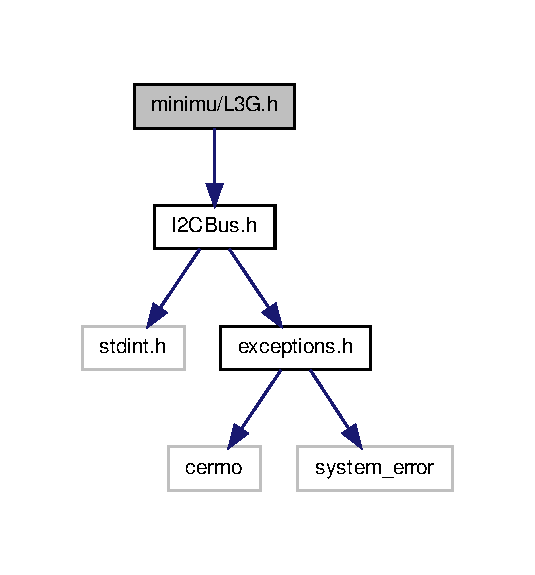
\includegraphics[width=257pt]{_l3_g_8h__incl}
\end{center}
\end{figure}
\-This graph shows which files directly or indirectly include this file\-:
\nopagebreak
\begin{figure}[H]
\begin{center}
\leavevmode
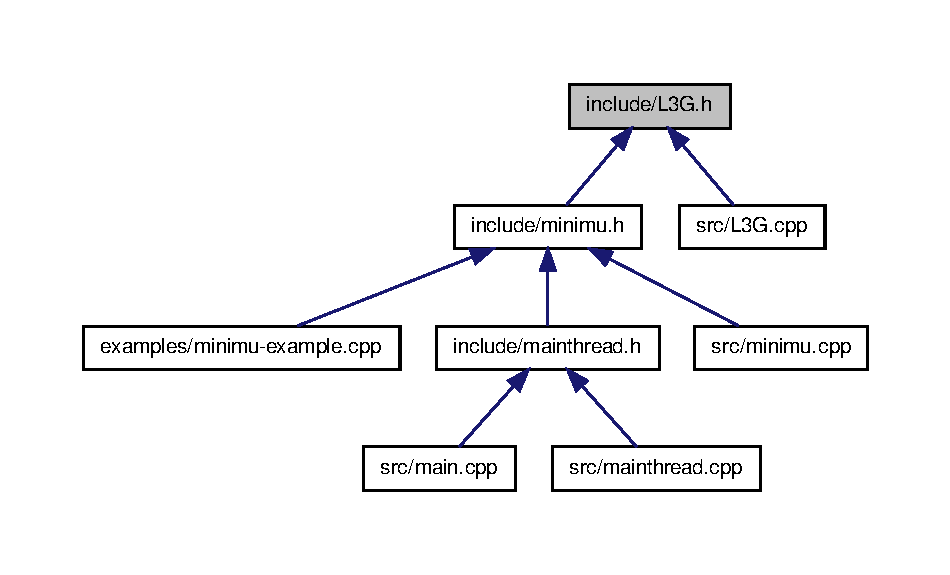
\includegraphics[width=350pt]{_l3_g_8h__dep__incl}
\end{center}
\end{figure}
\subsection*{\-Classes}
\begin{DoxyCompactItemize}
\item 
class \hyperlink{class_l3_g}{\-L3\-G}
\end{DoxyCompactItemize}
\subsection*{\-Defines}
\begin{DoxyCompactItemize}
\item 
\#define \hyperlink{_l3_g_8h_a170cb2b6f48b713af1c7bddf603ed09c}{\-L3\-G\-\_\-\-W\-H\-O\-\_\-\-A\-M\-\_\-\-I}~0x0\-F
\item 
\#define \hyperlink{_l3_g_8h_a30f840ff3b9fdfbcbfe6afa8c1c142de}{\-L3\-G\-\_\-\-C\-T\-R\-L\-\_\-\-R\-E\-G1}~0x20
\item 
\#define \hyperlink{_l3_g_8h_a0975625eb54e19d51faa141d5340a4e4}{\-L3\-G\-\_\-\-C\-T\-R\-L\-\_\-\-R\-E\-G2}~0x21
\item 
\#define \hyperlink{_l3_g_8h_a33248f4e864045f3658bee7371713a6e}{\-L3\-G\-\_\-\-C\-T\-R\-L\-\_\-\-R\-E\-G3}~0x22
\item 
\#define \hyperlink{_l3_g_8h_af2ecac824a6da5191218d6ecdaf16a1b}{\-L3\-G\-\_\-\-C\-T\-R\-L\-\_\-\-R\-E\-G4}~0x23
\item 
\#define \hyperlink{_l3_g_8h_a006f7a059ab0580738cf95a0e5b05bee}{\-L3\-G\-\_\-\-C\-T\-R\-L\-\_\-\-R\-E\-G5}~0x24
\item 
\#define \hyperlink{_l3_g_8h_afb8b70a1133d80234449f61bb8c7641a}{\-L3\-G\-\_\-\-R\-E\-F\-E\-R\-E\-N\-C\-E}~0x25
\item 
\#define \hyperlink{_l3_g_8h_a43f6311a260bd9f56fbfdba49623b870}{\-L3\-G\-\_\-\-O\-U\-T\-\_\-\-T\-E\-M\-P}~0x26
\item 
\#define \hyperlink{_l3_g_8h_a6f7b20f19c59f5f81c93ca71d60331ef}{\-L3\-G\-\_\-\-S\-T\-A\-T\-U\-S\-\_\-\-R\-E\-G}~0x27
\item 
\#define \hyperlink{_l3_g_8h_a8fa832687070bb2fb7f84afdc5b92529}{\-L3\-G\-\_\-\-O\-U\-T\-\_\-\-X\-\_\-\-L}~0x28
\item 
\#define \hyperlink{_l3_g_8h_ab84dd1b2edd783207800158149c16cfa}{\-L3\-G\-\_\-\-O\-U\-T\-\_\-\-X\-\_\-\-H}~0x29
\item 
\#define \hyperlink{_l3_g_8h_a3ae8bd9cc78f966469959d7709022619}{\-L3\-G\-\_\-\-O\-U\-T\-\_\-\-Y\-\_\-\-L}~0x2\-A
\item 
\#define \hyperlink{_l3_g_8h_a56730a646000a14f1cdf114848fb0816}{\-L3\-G\-\_\-\-O\-U\-T\-\_\-\-Y\-\_\-\-H}~0x2\-B
\item 
\#define \hyperlink{_l3_g_8h_a1c4be82ef69914f5b5f5890d8def43e9}{\-L3\-G\-\_\-\-O\-U\-T\-\_\-\-Z\-\_\-\-L}~0x2\-C
\item 
\#define \hyperlink{_l3_g_8h_ae45215f3e35b45515a7fb89cf54bcdcc}{\-L3\-G\-\_\-\-O\-U\-T\-\_\-\-Z\-\_\-\-H}~0x2\-D
\item 
\#define \hyperlink{_l3_g_8h_a01c72612003e3bf8f7ebc7bba1e3a689}{\-L3\-G\-\_\-\-F\-I\-F\-O\-\_\-\-C\-T\-R\-L\-\_\-\-R\-E\-G}~0x2\-E
\item 
\#define \hyperlink{_l3_g_8h_a556219ff899f9f5976e2855d675d1d2b}{\-L3\-G\-\_\-\-F\-I\-F\-O\-\_\-\-S\-R\-C\-\_\-\-R\-E\-G}~0x2\-F
\item 
\#define \hyperlink{_l3_g_8h_a0020020c5fd03618552d7ed4e6ef73da}{\-L3\-G\-\_\-\-I\-N\-T1\-\_\-\-C\-F\-G}~0x30
\item 
\#define \hyperlink{_l3_g_8h_a5315d323e8a68a3779714d6ac6188015}{\-L3\-G\-\_\-\-I\-N\-T1\-\_\-\-S\-R\-C}~0x31
\item 
\#define \hyperlink{_l3_g_8h_a4892bfd142867fcbbd2977deeaff9d89}{\-L3\-G\-\_\-\-I\-N\-T1\-\_\-\-T\-H\-S\-\_\-\-X\-H}~0x32
\item 
\#define \hyperlink{_l3_g_8h_afc0bced0bc6beea2819d28a4240c7e01}{\-L3\-G\-\_\-\-I\-N\-T1\-\_\-\-T\-H\-S\-\_\-\-X\-L}~0x33
\item 
\#define \hyperlink{_l3_g_8h_aa69f9044aa60166b6086d8a3b1669346}{\-L3\-G\-\_\-\-I\-N\-T1\-\_\-\-T\-H\-S\-\_\-\-Y\-H}~0x34
\item 
\#define \hyperlink{_l3_g_8h_a1964584415849020f8307601d9ebee37}{\-L3\-G\-\_\-\-I\-N\-T1\-\_\-\-T\-H\-S\-\_\-\-Y\-L}~0x35
\item 
\#define \hyperlink{_l3_g_8h_ae04a05e6b10e90f0cdeb5b035ee9508d}{\-L3\-G\-\_\-\-I\-N\-T1\-\_\-\-T\-H\-S\-\_\-\-Z\-H}~0x36
\item 
\#define \hyperlink{_l3_g_8h_ad6cf72648c0a11ee6aa242cd92e5f3d7}{\-L3\-G\-\_\-\-I\-N\-T1\-\_\-\-T\-H\-S\-\_\-\-Z\-L}~0x37
\item 
\#define \hyperlink{_l3_g_8h_a4a84dc4f988144bff2ee2ea4519e4648}{\-L3\-G\-\_\-\-I\-N\-T1\-\_\-\-D\-U\-R\-A\-T\-I\-O\-N}~0x38
\end{DoxyCompactItemize}


\subsection{\-Define \-Documentation}
\hypertarget{_l3_g_8h_a30f840ff3b9fdfbcbfe6afa8c1c142de}{\index{\-L3\-G.\-h@{\-L3\-G.\-h}!\-L3\-G\-\_\-\-C\-T\-R\-L\-\_\-\-R\-E\-G1@{\-L3\-G\-\_\-\-C\-T\-R\-L\-\_\-\-R\-E\-G1}}
\index{\-L3\-G\-\_\-\-C\-T\-R\-L\-\_\-\-R\-E\-G1@{\-L3\-G\-\_\-\-C\-T\-R\-L\-\_\-\-R\-E\-G1}!L3G.h@{\-L3\-G.\-h}}
\subsubsection[{\-L3\-G\-\_\-\-C\-T\-R\-L\-\_\-\-R\-E\-G1}]{\setlength{\rightskip}{0pt plus 5cm}\#define {\bf \-L3\-G\-\_\-\-C\-T\-R\-L\-\_\-\-R\-E\-G1}~0x20}}\label{_l3_g_8h_a30f840ff3b9fdfbcbfe6afa8c1c142de}


\-Definition at line 8 of file \-L3\-G.\-h.

\hypertarget{_l3_g_8h_a0975625eb54e19d51faa141d5340a4e4}{\index{\-L3\-G.\-h@{\-L3\-G.\-h}!\-L3\-G\-\_\-\-C\-T\-R\-L\-\_\-\-R\-E\-G2@{\-L3\-G\-\_\-\-C\-T\-R\-L\-\_\-\-R\-E\-G2}}
\index{\-L3\-G\-\_\-\-C\-T\-R\-L\-\_\-\-R\-E\-G2@{\-L3\-G\-\_\-\-C\-T\-R\-L\-\_\-\-R\-E\-G2}!L3G.h@{\-L3\-G.\-h}}
\subsubsection[{\-L3\-G\-\_\-\-C\-T\-R\-L\-\_\-\-R\-E\-G2}]{\setlength{\rightskip}{0pt plus 5cm}\#define {\bf \-L3\-G\-\_\-\-C\-T\-R\-L\-\_\-\-R\-E\-G2}~0x21}}\label{_l3_g_8h_a0975625eb54e19d51faa141d5340a4e4}


\-Definition at line 9 of file \-L3\-G.\-h.

\hypertarget{_l3_g_8h_a33248f4e864045f3658bee7371713a6e}{\index{\-L3\-G.\-h@{\-L3\-G.\-h}!\-L3\-G\-\_\-\-C\-T\-R\-L\-\_\-\-R\-E\-G3@{\-L3\-G\-\_\-\-C\-T\-R\-L\-\_\-\-R\-E\-G3}}
\index{\-L3\-G\-\_\-\-C\-T\-R\-L\-\_\-\-R\-E\-G3@{\-L3\-G\-\_\-\-C\-T\-R\-L\-\_\-\-R\-E\-G3}!L3G.h@{\-L3\-G.\-h}}
\subsubsection[{\-L3\-G\-\_\-\-C\-T\-R\-L\-\_\-\-R\-E\-G3}]{\setlength{\rightskip}{0pt plus 5cm}\#define {\bf \-L3\-G\-\_\-\-C\-T\-R\-L\-\_\-\-R\-E\-G3}~0x22}}\label{_l3_g_8h_a33248f4e864045f3658bee7371713a6e}


\-Definition at line 10 of file \-L3\-G.\-h.

\hypertarget{_l3_g_8h_af2ecac824a6da5191218d6ecdaf16a1b}{\index{\-L3\-G.\-h@{\-L3\-G.\-h}!\-L3\-G\-\_\-\-C\-T\-R\-L\-\_\-\-R\-E\-G4@{\-L3\-G\-\_\-\-C\-T\-R\-L\-\_\-\-R\-E\-G4}}
\index{\-L3\-G\-\_\-\-C\-T\-R\-L\-\_\-\-R\-E\-G4@{\-L3\-G\-\_\-\-C\-T\-R\-L\-\_\-\-R\-E\-G4}!L3G.h@{\-L3\-G.\-h}}
\subsubsection[{\-L3\-G\-\_\-\-C\-T\-R\-L\-\_\-\-R\-E\-G4}]{\setlength{\rightskip}{0pt plus 5cm}\#define {\bf \-L3\-G\-\_\-\-C\-T\-R\-L\-\_\-\-R\-E\-G4}~0x23}}\label{_l3_g_8h_af2ecac824a6da5191218d6ecdaf16a1b}


\-Definition at line 11 of file \-L3\-G.\-h.

\hypertarget{_l3_g_8h_a006f7a059ab0580738cf95a0e5b05bee}{\index{\-L3\-G.\-h@{\-L3\-G.\-h}!\-L3\-G\-\_\-\-C\-T\-R\-L\-\_\-\-R\-E\-G5@{\-L3\-G\-\_\-\-C\-T\-R\-L\-\_\-\-R\-E\-G5}}
\index{\-L3\-G\-\_\-\-C\-T\-R\-L\-\_\-\-R\-E\-G5@{\-L3\-G\-\_\-\-C\-T\-R\-L\-\_\-\-R\-E\-G5}!L3G.h@{\-L3\-G.\-h}}
\subsubsection[{\-L3\-G\-\_\-\-C\-T\-R\-L\-\_\-\-R\-E\-G5}]{\setlength{\rightskip}{0pt plus 5cm}\#define {\bf \-L3\-G\-\_\-\-C\-T\-R\-L\-\_\-\-R\-E\-G5}~0x24}}\label{_l3_g_8h_a006f7a059ab0580738cf95a0e5b05bee}


\-Definition at line 12 of file \-L3\-G.\-h.

\hypertarget{_l3_g_8h_a01c72612003e3bf8f7ebc7bba1e3a689}{\index{\-L3\-G.\-h@{\-L3\-G.\-h}!\-L3\-G\-\_\-\-F\-I\-F\-O\-\_\-\-C\-T\-R\-L\-\_\-\-R\-E\-G@{\-L3\-G\-\_\-\-F\-I\-F\-O\-\_\-\-C\-T\-R\-L\-\_\-\-R\-E\-G}}
\index{\-L3\-G\-\_\-\-F\-I\-F\-O\-\_\-\-C\-T\-R\-L\-\_\-\-R\-E\-G@{\-L3\-G\-\_\-\-F\-I\-F\-O\-\_\-\-C\-T\-R\-L\-\_\-\-R\-E\-G}!L3G.h@{\-L3\-G.\-h}}
\subsubsection[{\-L3\-G\-\_\-\-F\-I\-F\-O\-\_\-\-C\-T\-R\-L\-\_\-\-R\-E\-G}]{\setlength{\rightskip}{0pt plus 5cm}\#define {\bf \-L3\-G\-\_\-\-F\-I\-F\-O\-\_\-\-C\-T\-R\-L\-\_\-\-R\-E\-G}~0x2\-E}}\label{_l3_g_8h_a01c72612003e3bf8f7ebc7bba1e3a689}


\-Definition at line 24 of file \-L3\-G.\-h.

\hypertarget{_l3_g_8h_a556219ff899f9f5976e2855d675d1d2b}{\index{\-L3\-G.\-h@{\-L3\-G.\-h}!\-L3\-G\-\_\-\-F\-I\-F\-O\-\_\-\-S\-R\-C\-\_\-\-R\-E\-G@{\-L3\-G\-\_\-\-F\-I\-F\-O\-\_\-\-S\-R\-C\-\_\-\-R\-E\-G}}
\index{\-L3\-G\-\_\-\-F\-I\-F\-O\-\_\-\-S\-R\-C\-\_\-\-R\-E\-G@{\-L3\-G\-\_\-\-F\-I\-F\-O\-\_\-\-S\-R\-C\-\_\-\-R\-E\-G}!L3G.h@{\-L3\-G.\-h}}
\subsubsection[{\-L3\-G\-\_\-\-F\-I\-F\-O\-\_\-\-S\-R\-C\-\_\-\-R\-E\-G}]{\setlength{\rightskip}{0pt plus 5cm}\#define {\bf \-L3\-G\-\_\-\-F\-I\-F\-O\-\_\-\-S\-R\-C\-\_\-\-R\-E\-G}~0x2\-F}}\label{_l3_g_8h_a556219ff899f9f5976e2855d675d1d2b}


\-Definition at line 25 of file \-L3\-G.\-h.

\hypertarget{_l3_g_8h_a0020020c5fd03618552d7ed4e6ef73da}{\index{\-L3\-G.\-h@{\-L3\-G.\-h}!\-L3\-G\-\_\-\-I\-N\-T1\-\_\-\-C\-F\-G@{\-L3\-G\-\_\-\-I\-N\-T1\-\_\-\-C\-F\-G}}
\index{\-L3\-G\-\_\-\-I\-N\-T1\-\_\-\-C\-F\-G@{\-L3\-G\-\_\-\-I\-N\-T1\-\_\-\-C\-F\-G}!L3G.h@{\-L3\-G.\-h}}
\subsubsection[{\-L3\-G\-\_\-\-I\-N\-T1\-\_\-\-C\-F\-G}]{\setlength{\rightskip}{0pt plus 5cm}\#define {\bf \-L3\-G\-\_\-\-I\-N\-T1\-\_\-\-C\-F\-G}~0x30}}\label{_l3_g_8h_a0020020c5fd03618552d7ed4e6ef73da}


\-Definition at line 27 of file \-L3\-G.\-h.

\hypertarget{_l3_g_8h_a4a84dc4f988144bff2ee2ea4519e4648}{\index{\-L3\-G.\-h@{\-L3\-G.\-h}!\-L3\-G\-\_\-\-I\-N\-T1\-\_\-\-D\-U\-R\-A\-T\-I\-O\-N@{\-L3\-G\-\_\-\-I\-N\-T1\-\_\-\-D\-U\-R\-A\-T\-I\-O\-N}}
\index{\-L3\-G\-\_\-\-I\-N\-T1\-\_\-\-D\-U\-R\-A\-T\-I\-O\-N@{\-L3\-G\-\_\-\-I\-N\-T1\-\_\-\-D\-U\-R\-A\-T\-I\-O\-N}!L3G.h@{\-L3\-G.\-h}}
\subsubsection[{\-L3\-G\-\_\-\-I\-N\-T1\-\_\-\-D\-U\-R\-A\-T\-I\-O\-N}]{\setlength{\rightskip}{0pt plus 5cm}\#define {\bf \-L3\-G\-\_\-\-I\-N\-T1\-\_\-\-D\-U\-R\-A\-T\-I\-O\-N}~0x38}}\label{_l3_g_8h_a4a84dc4f988144bff2ee2ea4519e4648}


\-Definition at line 35 of file \-L3\-G.\-h.

\hypertarget{_l3_g_8h_a5315d323e8a68a3779714d6ac6188015}{\index{\-L3\-G.\-h@{\-L3\-G.\-h}!\-L3\-G\-\_\-\-I\-N\-T1\-\_\-\-S\-R\-C@{\-L3\-G\-\_\-\-I\-N\-T1\-\_\-\-S\-R\-C}}
\index{\-L3\-G\-\_\-\-I\-N\-T1\-\_\-\-S\-R\-C@{\-L3\-G\-\_\-\-I\-N\-T1\-\_\-\-S\-R\-C}!L3G.h@{\-L3\-G.\-h}}
\subsubsection[{\-L3\-G\-\_\-\-I\-N\-T1\-\_\-\-S\-R\-C}]{\setlength{\rightskip}{0pt plus 5cm}\#define {\bf \-L3\-G\-\_\-\-I\-N\-T1\-\_\-\-S\-R\-C}~0x31}}\label{_l3_g_8h_a5315d323e8a68a3779714d6ac6188015}


\-Definition at line 28 of file \-L3\-G.\-h.

\hypertarget{_l3_g_8h_a4892bfd142867fcbbd2977deeaff9d89}{\index{\-L3\-G.\-h@{\-L3\-G.\-h}!\-L3\-G\-\_\-\-I\-N\-T1\-\_\-\-T\-H\-S\-\_\-\-X\-H@{\-L3\-G\-\_\-\-I\-N\-T1\-\_\-\-T\-H\-S\-\_\-\-X\-H}}
\index{\-L3\-G\-\_\-\-I\-N\-T1\-\_\-\-T\-H\-S\-\_\-\-X\-H@{\-L3\-G\-\_\-\-I\-N\-T1\-\_\-\-T\-H\-S\-\_\-\-X\-H}!L3G.h@{\-L3\-G.\-h}}
\subsubsection[{\-L3\-G\-\_\-\-I\-N\-T1\-\_\-\-T\-H\-S\-\_\-\-X\-H}]{\setlength{\rightskip}{0pt plus 5cm}\#define {\bf \-L3\-G\-\_\-\-I\-N\-T1\-\_\-\-T\-H\-S\-\_\-\-X\-H}~0x32}}\label{_l3_g_8h_a4892bfd142867fcbbd2977deeaff9d89}


\-Definition at line 29 of file \-L3\-G.\-h.

\hypertarget{_l3_g_8h_afc0bced0bc6beea2819d28a4240c7e01}{\index{\-L3\-G.\-h@{\-L3\-G.\-h}!\-L3\-G\-\_\-\-I\-N\-T1\-\_\-\-T\-H\-S\-\_\-\-X\-L@{\-L3\-G\-\_\-\-I\-N\-T1\-\_\-\-T\-H\-S\-\_\-\-X\-L}}
\index{\-L3\-G\-\_\-\-I\-N\-T1\-\_\-\-T\-H\-S\-\_\-\-X\-L@{\-L3\-G\-\_\-\-I\-N\-T1\-\_\-\-T\-H\-S\-\_\-\-X\-L}!L3G.h@{\-L3\-G.\-h}}
\subsubsection[{\-L3\-G\-\_\-\-I\-N\-T1\-\_\-\-T\-H\-S\-\_\-\-X\-L}]{\setlength{\rightskip}{0pt plus 5cm}\#define {\bf \-L3\-G\-\_\-\-I\-N\-T1\-\_\-\-T\-H\-S\-\_\-\-X\-L}~0x33}}\label{_l3_g_8h_afc0bced0bc6beea2819d28a4240c7e01}


\-Definition at line 30 of file \-L3\-G.\-h.

\hypertarget{_l3_g_8h_aa69f9044aa60166b6086d8a3b1669346}{\index{\-L3\-G.\-h@{\-L3\-G.\-h}!\-L3\-G\-\_\-\-I\-N\-T1\-\_\-\-T\-H\-S\-\_\-\-Y\-H@{\-L3\-G\-\_\-\-I\-N\-T1\-\_\-\-T\-H\-S\-\_\-\-Y\-H}}
\index{\-L3\-G\-\_\-\-I\-N\-T1\-\_\-\-T\-H\-S\-\_\-\-Y\-H@{\-L3\-G\-\_\-\-I\-N\-T1\-\_\-\-T\-H\-S\-\_\-\-Y\-H}!L3G.h@{\-L3\-G.\-h}}
\subsubsection[{\-L3\-G\-\_\-\-I\-N\-T1\-\_\-\-T\-H\-S\-\_\-\-Y\-H}]{\setlength{\rightskip}{0pt plus 5cm}\#define {\bf \-L3\-G\-\_\-\-I\-N\-T1\-\_\-\-T\-H\-S\-\_\-\-Y\-H}~0x34}}\label{_l3_g_8h_aa69f9044aa60166b6086d8a3b1669346}


\-Definition at line 31 of file \-L3\-G.\-h.

\hypertarget{_l3_g_8h_a1964584415849020f8307601d9ebee37}{\index{\-L3\-G.\-h@{\-L3\-G.\-h}!\-L3\-G\-\_\-\-I\-N\-T1\-\_\-\-T\-H\-S\-\_\-\-Y\-L@{\-L3\-G\-\_\-\-I\-N\-T1\-\_\-\-T\-H\-S\-\_\-\-Y\-L}}
\index{\-L3\-G\-\_\-\-I\-N\-T1\-\_\-\-T\-H\-S\-\_\-\-Y\-L@{\-L3\-G\-\_\-\-I\-N\-T1\-\_\-\-T\-H\-S\-\_\-\-Y\-L}!L3G.h@{\-L3\-G.\-h}}
\subsubsection[{\-L3\-G\-\_\-\-I\-N\-T1\-\_\-\-T\-H\-S\-\_\-\-Y\-L}]{\setlength{\rightskip}{0pt plus 5cm}\#define {\bf \-L3\-G\-\_\-\-I\-N\-T1\-\_\-\-T\-H\-S\-\_\-\-Y\-L}~0x35}}\label{_l3_g_8h_a1964584415849020f8307601d9ebee37}


\-Definition at line 32 of file \-L3\-G.\-h.

\hypertarget{_l3_g_8h_ae04a05e6b10e90f0cdeb5b035ee9508d}{\index{\-L3\-G.\-h@{\-L3\-G.\-h}!\-L3\-G\-\_\-\-I\-N\-T1\-\_\-\-T\-H\-S\-\_\-\-Z\-H@{\-L3\-G\-\_\-\-I\-N\-T1\-\_\-\-T\-H\-S\-\_\-\-Z\-H}}
\index{\-L3\-G\-\_\-\-I\-N\-T1\-\_\-\-T\-H\-S\-\_\-\-Z\-H@{\-L3\-G\-\_\-\-I\-N\-T1\-\_\-\-T\-H\-S\-\_\-\-Z\-H}!L3G.h@{\-L3\-G.\-h}}
\subsubsection[{\-L3\-G\-\_\-\-I\-N\-T1\-\_\-\-T\-H\-S\-\_\-\-Z\-H}]{\setlength{\rightskip}{0pt plus 5cm}\#define {\bf \-L3\-G\-\_\-\-I\-N\-T1\-\_\-\-T\-H\-S\-\_\-\-Z\-H}~0x36}}\label{_l3_g_8h_ae04a05e6b10e90f0cdeb5b035ee9508d}


\-Definition at line 33 of file \-L3\-G.\-h.

\hypertarget{_l3_g_8h_ad6cf72648c0a11ee6aa242cd92e5f3d7}{\index{\-L3\-G.\-h@{\-L3\-G.\-h}!\-L3\-G\-\_\-\-I\-N\-T1\-\_\-\-T\-H\-S\-\_\-\-Z\-L@{\-L3\-G\-\_\-\-I\-N\-T1\-\_\-\-T\-H\-S\-\_\-\-Z\-L}}
\index{\-L3\-G\-\_\-\-I\-N\-T1\-\_\-\-T\-H\-S\-\_\-\-Z\-L@{\-L3\-G\-\_\-\-I\-N\-T1\-\_\-\-T\-H\-S\-\_\-\-Z\-L}!L3G.h@{\-L3\-G.\-h}}
\subsubsection[{\-L3\-G\-\_\-\-I\-N\-T1\-\_\-\-T\-H\-S\-\_\-\-Z\-L}]{\setlength{\rightskip}{0pt plus 5cm}\#define {\bf \-L3\-G\-\_\-\-I\-N\-T1\-\_\-\-T\-H\-S\-\_\-\-Z\-L}~0x37}}\label{_l3_g_8h_ad6cf72648c0a11ee6aa242cd92e5f3d7}


\-Definition at line 34 of file \-L3\-G.\-h.

\hypertarget{_l3_g_8h_a43f6311a260bd9f56fbfdba49623b870}{\index{\-L3\-G.\-h@{\-L3\-G.\-h}!\-L3\-G\-\_\-\-O\-U\-T\-\_\-\-T\-E\-M\-P@{\-L3\-G\-\_\-\-O\-U\-T\-\_\-\-T\-E\-M\-P}}
\index{\-L3\-G\-\_\-\-O\-U\-T\-\_\-\-T\-E\-M\-P@{\-L3\-G\-\_\-\-O\-U\-T\-\_\-\-T\-E\-M\-P}!L3G.h@{\-L3\-G.\-h}}
\subsubsection[{\-L3\-G\-\_\-\-O\-U\-T\-\_\-\-T\-E\-M\-P}]{\setlength{\rightskip}{0pt plus 5cm}\#define {\bf \-L3\-G\-\_\-\-O\-U\-T\-\_\-\-T\-E\-M\-P}~0x26}}\label{_l3_g_8h_a43f6311a260bd9f56fbfdba49623b870}


\-Definition at line 14 of file \-L3\-G.\-h.

\hypertarget{_l3_g_8h_ab84dd1b2edd783207800158149c16cfa}{\index{\-L3\-G.\-h@{\-L3\-G.\-h}!\-L3\-G\-\_\-\-O\-U\-T\-\_\-\-X\-\_\-\-H@{\-L3\-G\-\_\-\-O\-U\-T\-\_\-\-X\-\_\-\-H}}
\index{\-L3\-G\-\_\-\-O\-U\-T\-\_\-\-X\-\_\-\-H@{\-L3\-G\-\_\-\-O\-U\-T\-\_\-\-X\-\_\-\-H}!L3G.h@{\-L3\-G.\-h}}
\subsubsection[{\-L3\-G\-\_\-\-O\-U\-T\-\_\-\-X\-\_\-\-H}]{\setlength{\rightskip}{0pt plus 5cm}\#define {\bf \-L3\-G\-\_\-\-O\-U\-T\-\_\-\-X\-\_\-\-H}~0x29}}\label{_l3_g_8h_ab84dd1b2edd783207800158149c16cfa}


\-Definition at line 18 of file \-L3\-G.\-h.

\hypertarget{_l3_g_8h_a8fa832687070bb2fb7f84afdc5b92529}{\index{\-L3\-G.\-h@{\-L3\-G.\-h}!\-L3\-G\-\_\-\-O\-U\-T\-\_\-\-X\-\_\-\-L@{\-L3\-G\-\_\-\-O\-U\-T\-\_\-\-X\-\_\-\-L}}
\index{\-L3\-G\-\_\-\-O\-U\-T\-\_\-\-X\-\_\-\-L@{\-L3\-G\-\_\-\-O\-U\-T\-\_\-\-X\-\_\-\-L}!L3G.h@{\-L3\-G.\-h}}
\subsubsection[{\-L3\-G\-\_\-\-O\-U\-T\-\_\-\-X\-\_\-\-L}]{\setlength{\rightskip}{0pt plus 5cm}\#define {\bf \-L3\-G\-\_\-\-O\-U\-T\-\_\-\-X\-\_\-\-L}~0x28}}\label{_l3_g_8h_a8fa832687070bb2fb7f84afdc5b92529}


\-Definition at line 17 of file \-L3\-G.\-h.

\hypertarget{_l3_g_8h_a56730a646000a14f1cdf114848fb0816}{\index{\-L3\-G.\-h@{\-L3\-G.\-h}!\-L3\-G\-\_\-\-O\-U\-T\-\_\-\-Y\-\_\-\-H@{\-L3\-G\-\_\-\-O\-U\-T\-\_\-\-Y\-\_\-\-H}}
\index{\-L3\-G\-\_\-\-O\-U\-T\-\_\-\-Y\-\_\-\-H@{\-L3\-G\-\_\-\-O\-U\-T\-\_\-\-Y\-\_\-\-H}!L3G.h@{\-L3\-G.\-h}}
\subsubsection[{\-L3\-G\-\_\-\-O\-U\-T\-\_\-\-Y\-\_\-\-H}]{\setlength{\rightskip}{0pt plus 5cm}\#define {\bf \-L3\-G\-\_\-\-O\-U\-T\-\_\-\-Y\-\_\-\-H}~0x2\-B}}\label{_l3_g_8h_a56730a646000a14f1cdf114848fb0816}


\-Definition at line 20 of file \-L3\-G.\-h.

\hypertarget{_l3_g_8h_a3ae8bd9cc78f966469959d7709022619}{\index{\-L3\-G.\-h@{\-L3\-G.\-h}!\-L3\-G\-\_\-\-O\-U\-T\-\_\-\-Y\-\_\-\-L@{\-L3\-G\-\_\-\-O\-U\-T\-\_\-\-Y\-\_\-\-L}}
\index{\-L3\-G\-\_\-\-O\-U\-T\-\_\-\-Y\-\_\-\-L@{\-L3\-G\-\_\-\-O\-U\-T\-\_\-\-Y\-\_\-\-L}!L3G.h@{\-L3\-G.\-h}}
\subsubsection[{\-L3\-G\-\_\-\-O\-U\-T\-\_\-\-Y\-\_\-\-L}]{\setlength{\rightskip}{0pt plus 5cm}\#define {\bf \-L3\-G\-\_\-\-O\-U\-T\-\_\-\-Y\-\_\-\-L}~0x2\-A}}\label{_l3_g_8h_a3ae8bd9cc78f966469959d7709022619}


\-Definition at line 19 of file \-L3\-G.\-h.

\hypertarget{_l3_g_8h_ae45215f3e35b45515a7fb89cf54bcdcc}{\index{\-L3\-G.\-h@{\-L3\-G.\-h}!\-L3\-G\-\_\-\-O\-U\-T\-\_\-\-Z\-\_\-\-H@{\-L3\-G\-\_\-\-O\-U\-T\-\_\-\-Z\-\_\-\-H}}
\index{\-L3\-G\-\_\-\-O\-U\-T\-\_\-\-Z\-\_\-\-H@{\-L3\-G\-\_\-\-O\-U\-T\-\_\-\-Z\-\_\-\-H}!L3G.h@{\-L3\-G.\-h}}
\subsubsection[{\-L3\-G\-\_\-\-O\-U\-T\-\_\-\-Z\-\_\-\-H}]{\setlength{\rightskip}{0pt plus 5cm}\#define {\bf \-L3\-G\-\_\-\-O\-U\-T\-\_\-\-Z\-\_\-\-H}~0x2\-D}}\label{_l3_g_8h_ae45215f3e35b45515a7fb89cf54bcdcc}


\-Definition at line 22 of file \-L3\-G.\-h.

\hypertarget{_l3_g_8h_a1c4be82ef69914f5b5f5890d8def43e9}{\index{\-L3\-G.\-h@{\-L3\-G.\-h}!\-L3\-G\-\_\-\-O\-U\-T\-\_\-\-Z\-\_\-\-L@{\-L3\-G\-\_\-\-O\-U\-T\-\_\-\-Z\-\_\-\-L}}
\index{\-L3\-G\-\_\-\-O\-U\-T\-\_\-\-Z\-\_\-\-L@{\-L3\-G\-\_\-\-O\-U\-T\-\_\-\-Z\-\_\-\-L}!L3G.h@{\-L3\-G.\-h}}
\subsubsection[{\-L3\-G\-\_\-\-O\-U\-T\-\_\-\-Z\-\_\-\-L}]{\setlength{\rightskip}{0pt plus 5cm}\#define {\bf \-L3\-G\-\_\-\-O\-U\-T\-\_\-\-Z\-\_\-\-L}~0x2\-C}}\label{_l3_g_8h_a1c4be82ef69914f5b5f5890d8def43e9}


\-Definition at line 21 of file \-L3\-G.\-h.

\hypertarget{_l3_g_8h_afb8b70a1133d80234449f61bb8c7641a}{\index{\-L3\-G.\-h@{\-L3\-G.\-h}!\-L3\-G\-\_\-\-R\-E\-F\-E\-R\-E\-N\-C\-E@{\-L3\-G\-\_\-\-R\-E\-F\-E\-R\-E\-N\-C\-E}}
\index{\-L3\-G\-\_\-\-R\-E\-F\-E\-R\-E\-N\-C\-E@{\-L3\-G\-\_\-\-R\-E\-F\-E\-R\-E\-N\-C\-E}!L3G.h@{\-L3\-G.\-h}}
\subsubsection[{\-L3\-G\-\_\-\-R\-E\-F\-E\-R\-E\-N\-C\-E}]{\setlength{\rightskip}{0pt plus 5cm}\#define {\bf \-L3\-G\-\_\-\-R\-E\-F\-E\-R\-E\-N\-C\-E}~0x25}}\label{_l3_g_8h_afb8b70a1133d80234449f61bb8c7641a}


\-Definition at line 13 of file \-L3\-G.\-h.

\hypertarget{_l3_g_8h_a6f7b20f19c59f5f81c93ca71d60331ef}{\index{\-L3\-G.\-h@{\-L3\-G.\-h}!\-L3\-G\-\_\-\-S\-T\-A\-T\-U\-S\-\_\-\-R\-E\-G@{\-L3\-G\-\_\-\-S\-T\-A\-T\-U\-S\-\_\-\-R\-E\-G}}
\index{\-L3\-G\-\_\-\-S\-T\-A\-T\-U\-S\-\_\-\-R\-E\-G@{\-L3\-G\-\_\-\-S\-T\-A\-T\-U\-S\-\_\-\-R\-E\-G}!L3G.h@{\-L3\-G.\-h}}
\subsubsection[{\-L3\-G\-\_\-\-S\-T\-A\-T\-U\-S\-\_\-\-R\-E\-G}]{\setlength{\rightskip}{0pt plus 5cm}\#define {\bf \-L3\-G\-\_\-\-S\-T\-A\-T\-U\-S\-\_\-\-R\-E\-G}~0x27}}\label{_l3_g_8h_a6f7b20f19c59f5f81c93ca71d60331ef}


\-Definition at line 15 of file \-L3\-G.\-h.

\hypertarget{_l3_g_8h_a170cb2b6f48b713af1c7bddf603ed09c}{\index{\-L3\-G.\-h@{\-L3\-G.\-h}!\-L3\-G\-\_\-\-W\-H\-O\-\_\-\-A\-M\-\_\-\-I@{\-L3\-G\-\_\-\-W\-H\-O\-\_\-\-A\-M\-\_\-\-I}}
\index{\-L3\-G\-\_\-\-W\-H\-O\-\_\-\-A\-M\-\_\-\-I@{\-L3\-G\-\_\-\-W\-H\-O\-\_\-\-A\-M\-\_\-\-I}!L3G.h@{\-L3\-G.\-h}}
\subsubsection[{\-L3\-G\-\_\-\-W\-H\-O\-\_\-\-A\-M\-\_\-\-I}]{\setlength{\rightskip}{0pt plus 5cm}\#define {\bf \-L3\-G\-\_\-\-W\-H\-O\-\_\-\-A\-M\-\_\-\-I}~0x0\-F}}\label{_l3_g_8h_a170cb2b6f48b713af1c7bddf603ed09c}


\-Definition at line 6 of file \-L3\-G.\-h.


\hypertarget{_l_s_m303_8cpp}{\section{src/\-L\-S\-M303.cpp \-File \-Reference}
\label{_l_s_m303_8cpp}\index{src/\-L\-S\-M303.\-cpp@{src/\-L\-S\-M303.\-cpp}}
}
{\ttfamily \#include \char`\"{}\-L\-S\-M303.\-h\char`\"{}}\*
\-Include dependency graph for \-L\-S\-M303.\-cpp\-:
\nopagebreak
\begin{figure}[H]
\begin{center}
\leavevmode
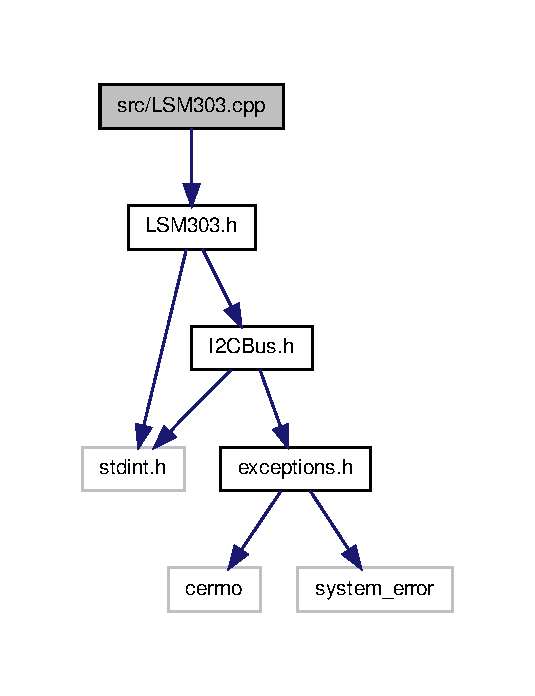
\includegraphics[width=257pt]{_l_s_m303_8cpp__incl}
\end{center}
\end{figure}
\subsection*{\-Defines}
\begin{DoxyCompactItemize}
\item 
\#define \hyperlink{_l_s_m303_8cpp_ade4e63fac819c67040e374f08d2d7230}{\-M\-A\-G\-\_\-\-A\-D\-D\-R\-E\-S\-S}~(0x3\-C $>$$>$ 1)
\item 
\#define \hyperlink{_l_s_m303_8cpp_a44d83da6f81354e553d574e99ee0691e}{\-A\-C\-C\-\_\-\-A\-D\-D\-R\-E\-S\-S\-\_\-\-S\-A0\-\_\-\-A\-\_\-\-L\-O\-W}~(0x30 $>$$>$ 1)
\item 
\#define \hyperlink{_l_s_m303_8cpp_aa938ef5c958ad633f62e45ce3eda5054}{\-A\-C\-C\-\_\-\-A\-D\-D\-R\-E\-S\-S\-\_\-\-S\-A0\-\_\-\-A\-\_\-\-H\-I\-G\-H}~(0x32 $>$$>$ 1)
\end{DoxyCompactItemize}


\subsection{\-Define \-Documentation}
\hypertarget{_l_s_m303_8cpp_aa938ef5c958ad633f62e45ce3eda5054}{\index{\-L\-S\-M303.\-cpp@{\-L\-S\-M303.\-cpp}!\-A\-C\-C\-\_\-\-A\-D\-D\-R\-E\-S\-S\-\_\-\-S\-A0\-\_\-\-A\-\_\-\-H\-I\-G\-H@{\-A\-C\-C\-\_\-\-A\-D\-D\-R\-E\-S\-S\-\_\-\-S\-A0\-\_\-\-A\-\_\-\-H\-I\-G\-H}}
\index{\-A\-C\-C\-\_\-\-A\-D\-D\-R\-E\-S\-S\-\_\-\-S\-A0\-\_\-\-A\-\_\-\-H\-I\-G\-H@{\-A\-C\-C\-\_\-\-A\-D\-D\-R\-E\-S\-S\-\_\-\-S\-A0\-\_\-\-A\-\_\-\-H\-I\-G\-H}!LSM303.cpp@{\-L\-S\-M303.\-cpp}}
\subsubsection[{\-A\-C\-C\-\_\-\-A\-D\-D\-R\-E\-S\-S\-\_\-\-S\-A0\-\_\-\-A\-\_\-\-H\-I\-G\-H}]{\setlength{\rightskip}{0pt plus 5cm}\#define {\bf \-A\-C\-C\-\_\-\-A\-D\-D\-R\-E\-S\-S\-\_\-\-S\-A0\-\_\-\-A\-\_\-\-H\-I\-G\-H}~(0x32 $>$$>$ 1)}}\label{_l_s_m303_8cpp_aa938ef5c958ad633f62e45ce3eda5054}


\-Definition at line 20 of file \-L\-S\-M303.\-cpp.

\hypertarget{_l_s_m303_8cpp_a44d83da6f81354e553d574e99ee0691e}{\index{\-L\-S\-M303.\-cpp@{\-L\-S\-M303.\-cpp}!\-A\-C\-C\-\_\-\-A\-D\-D\-R\-E\-S\-S\-\_\-\-S\-A0\-\_\-\-A\-\_\-\-L\-O\-W@{\-A\-C\-C\-\_\-\-A\-D\-D\-R\-E\-S\-S\-\_\-\-S\-A0\-\_\-\-A\-\_\-\-L\-O\-W}}
\index{\-A\-C\-C\-\_\-\-A\-D\-D\-R\-E\-S\-S\-\_\-\-S\-A0\-\_\-\-A\-\_\-\-L\-O\-W@{\-A\-C\-C\-\_\-\-A\-D\-D\-R\-E\-S\-S\-\_\-\-S\-A0\-\_\-\-A\-\_\-\-L\-O\-W}!LSM303.cpp@{\-L\-S\-M303.\-cpp}}
\subsubsection[{\-A\-C\-C\-\_\-\-A\-D\-D\-R\-E\-S\-S\-\_\-\-S\-A0\-\_\-\-A\-\_\-\-L\-O\-W}]{\setlength{\rightskip}{0pt plus 5cm}\#define {\bf \-A\-C\-C\-\_\-\-A\-D\-D\-R\-E\-S\-S\-\_\-\-S\-A0\-\_\-\-A\-\_\-\-L\-O\-W}~(0x30 $>$$>$ 1)}}\label{_l_s_m303_8cpp_a44d83da6f81354e553d574e99ee0691e}


\-Definition at line 19 of file \-L\-S\-M303.\-cpp.

\hypertarget{_l_s_m303_8cpp_ade4e63fac819c67040e374f08d2d7230}{\index{\-L\-S\-M303.\-cpp@{\-L\-S\-M303.\-cpp}!\-M\-A\-G\-\_\-\-A\-D\-D\-R\-E\-S\-S@{\-M\-A\-G\-\_\-\-A\-D\-D\-R\-E\-S\-S}}
\index{\-M\-A\-G\-\_\-\-A\-D\-D\-R\-E\-S\-S@{\-M\-A\-G\-\_\-\-A\-D\-D\-R\-E\-S\-S}!LSM303.cpp@{\-L\-S\-M303.\-cpp}}
\subsubsection[{\-M\-A\-G\-\_\-\-A\-D\-D\-R\-E\-S\-S}]{\setlength{\rightskip}{0pt plus 5cm}\#define {\bf \-M\-A\-G\-\_\-\-A\-D\-D\-R\-E\-S\-S}~(0x3\-C $>$$>$ 1)}}\label{_l_s_m303_8cpp_ade4e63fac819c67040e374f08d2d7230}


\-Definition at line 18 of file \-L\-S\-M303.\-cpp.


\hypertarget{_l_s_m303_8h}{\section{minimu/\-L\-S\-M303.h \-File \-Reference}
\label{_l_s_m303_8h}\index{minimu/\-L\-S\-M303.\-h@{minimu/\-L\-S\-M303.\-h}}
}
{\ttfamily \#include $<$stdint.\-h$>$}\*
{\ttfamily \#include \char`\"{}\-I2\-C\-Bus.\-h\char`\"{}}\*
\-Include dependency graph for \-L\-S\-M303.\-h\-:
\nopagebreak
\begin{figure}[H]
\begin{center}
\leavevmode
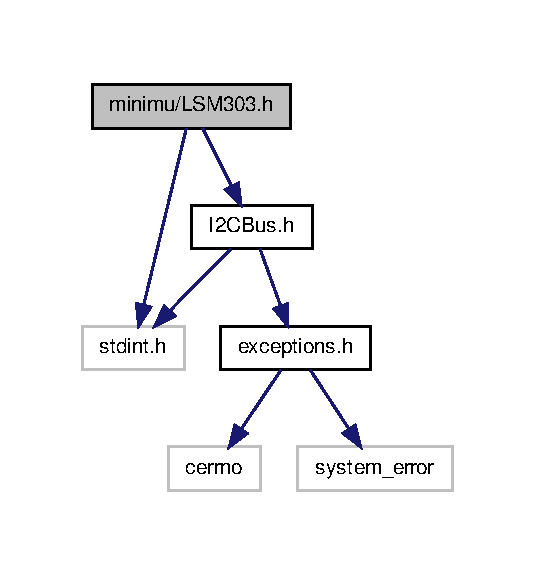
\includegraphics[width=257pt]{_l_s_m303_8h__incl}
\end{center}
\end{figure}
\-This graph shows which files directly or indirectly include this file\-:
\nopagebreak
\begin{figure}[H]
\begin{center}
\leavevmode
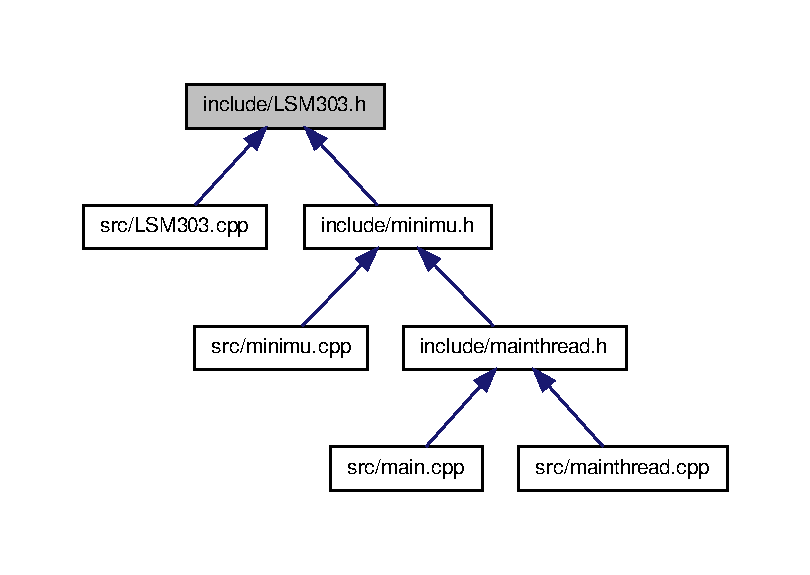
\includegraphics[width=350pt]{_l_s_m303_8h__dep__incl}
\end{center}
\end{figure}
\subsection*{\-Classes}
\begin{DoxyCompactItemize}
\item 
class \hyperlink{class_l_s_m303}{\-L\-S\-M303}
\end{DoxyCompactItemize}
\subsection*{\-Defines}
\begin{DoxyCompactItemize}
\item 
\#define \hyperlink{_l_s_m303_8h_a7bc2e580518a6f05f7ca0efb8cd4f901}{\-L\-S\-M303\-\_\-\-C\-T\-R\-L\-\_\-\-R\-E\-G1\-\_\-\-A}~0x20
\item 
\#define \hyperlink{_l_s_m303_8h_ae9707504c0fd20dbf541dd8dbb00ad03}{\-L\-S\-M303\-\_\-\-C\-T\-R\-L\-\_\-\-R\-E\-G2\-\_\-\-A}~0x21
\item 
\#define \hyperlink{_l_s_m303_8h_a6943930d7df7faaa36f037fbc8c7fc8e}{\-L\-S\-M303\-\_\-\-C\-T\-R\-L\-\_\-\-R\-E\-G3\-\_\-\-A}~0x22
\item 
\#define \hyperlink{_l_s_m303_8h_a063526d36f5ae338ef52a739f86bb78e}{\-L\-S\-M303\-\_\-\-C\-T\-R\-L\-\_\-\-R\-E\-G4\-\_\-\-A}~0x23
\item 
\#define \hyperlink{_l_s_m303_8h_a2f2ef9bd37abb445873b599c26367a13}{\-L\-S\-M303\-\_\-\-C\-T\-R\-L\-\_\-\-R\-E\-G5\-\_\-\-A}~0x24
\item 
\#define \hyperlink{_l_s_m303_8h_aa17d946ca73efa77acd933ae9e48e03a}{\-L\-S\-M303\-\_\-\-C\-T\-R\-L\-\_\-\-R\-E\-G6\-\_\-\-A}~0x25
\item 
\#define \hyperlink{_l_s_m303_8h_aa5e26647dc0e82e47ddd0e85280d86e3}{\-L\-S\-M303\-\_\-\-H\-P\-\_\-\-F\-I\-L\-T\-E\-R\-\_\-\-R\-E\-S\-E\-T\-\_\-\-A}~0x25
\item 
\#define \hyperlink{_l_s_m303_8h_abc6dcbcd71905c1f66882b81a168e326}{\-L\-S\-M303\-\_\-\-R\-E\-F\-E\-R\-E\-N\-C\-E\-\_\-\-A}~0x26
\item 
\#define \hyperlink{_l_s_m303_8h_ac994130e1fe795a4cd33a900456b9a41}{\-L\-S\-M303\-\_\-\-S\-T\-A\-T\-U\-S\-\_\-\-R\-E\-G\-\_\-\-A}~0x27
\item 
\#define \hyperlink{_l_s_m303_8h_aa3c0ec8694ee355ca488ff6913068501}{\-L\-S\-M303\-\_\-\-O\-U\-T\-\_\-\-X\-\_\-\-L\-\_\-\-A}~0x28
\item 
\#define \hyperlink{_l_s_m303_8h_afc10f981c3556a82a6326c282b0bb3f8}{\-L\-S\-M303\-\_\-\-O\-U\-T\-\_\-\-X\-\_\-\-H\-\_\-\-A}~0x29
\item 
\#define \hyperlink{_l_s_m303_8h_abd59972dfde7f616cc99d9e20e583073}{\-L\-S\-M303\-\_\-\-O\-U\-T\-\_\-\-Y\-\_\-\-L\-\_\-\-A}~0x2\-A
\item 
\#define \hyperlink{_l_s_m303_8h_a40eab40e1b6637ed43aa4b379a4f0ebe}{\-L\-S\-M303\-\_\-\-O\-U\-T\-\_\-\-Y\-\_\-\-H\-\_\-\-A}~0x2\-B
\item 
\#define \hyperlink{_l_s_m303_8h_a8e8cb2a97a71454ae1412bbd62ffb5f5}{\-L\-S\-M303\-\_\-\-O\-U\-T\-\_\-\-Z\-\_\-\-L\-\_\-\-A}~0x2\-C
\item 
\#define \hyperlink{_l_s_m303_8h_adb2f10a0ebaf0efa07d878a8a53f0de1}{\-L\-S\-M303\-\_\-\-O\-U\-T\-\_\-\-Z\-\_\-\-H\-\_\-\-A}~0x2\-D
\item 
\#define \hyperlink{_l_s_m303_8h_a14c0260aca12d4c51b1c8f666ba08d85}{\-L\-S\-M303\-\_\-\-F\-I\-F\-O\-\_\-\-C\-T\-R\-L\-\_\-\-R\-E\-G\-\_\-\-A}~0x2\-E
\item 
\#define \hyperlink{_l_s_m303_8h_a8b49ae212a73b5e05b54a216f4d942ad}{\-L\-S\-M303\-\_\-\-F\-I\-F\-O\-\_\-\-S\-R\-C\-\_\-\-R\-E\-G\-\_\-\-A}~0x2\-F
\item 
\#define \hyperlink{_l_s_m303_8h_a3d87d65452e1615f42ba28c6a1df6ae0}{\-L\-S\-M303\-\_\-\-I\-N\-T1\-\_\-\-C\-F\-G\-\_\-\-A}~0x30
\item 
\#define \hyperlink{_l_s_m303_8h_a36384a7381e872a021c55a7c5a64c83e}{\-L\-S\-M303\-\_\-\-I\-N\-T1\-\_\-\-S\-R\-C\-\_\-\-A}~0x31
\item 
\#define \hyperlink{_l_s_m303_8h_ae9c987f1918eb104ef6d8f80323ee0e2}{\-L\-S\-M303\-\_\-\-I\-N\-T1\-\_\-\-T\-H\-S\-\_\-\-A}~0x32
\item 
\#define \hyperlink{_l_s_m303_8h_a10b3f003690fd967f2d20b4755874cae}{\-L\-S\-M303\-\_\-\-I\-N\-T1\-\_\-\-D\-U\-R\-A\-T\-I\-O\-N\-\_\-\-A}~0x33
\item 
\#define \hyperlink{_l_s_m303_8h_ab628182b21ec8ad113ed7373f822025c}{\-L\-S\-M303\-\_\-\-I\-N\-T2\-\_\-\-C\-F\-G\-\_\-\-A}~0x34
\item 
\#define \hyperlink{_l_s_m303_8h_ae942d6737872f8bbdc698ebc08312cf1}{\-L\-S\-M303\-\_\-\-I\-N\-T2\-\_\-\-S\-R\-C\-\_\-\-A}~0x35
\item 
\#define \hyperlink{_l_s_m303_8h_a41f056377fb5c31a06b9405fd8a6a04d}{\-L\-S\-M303\-\_\-\-I\-N\-T2\-\_\-\-T\-H\-S\-\_\-\-A}~0x36
\item 
\#define \hyperlink{_l_s_m303_8h_afb6f5b7489d1df9dbb514491d9ceb307}{\-L\-S\-M303\-\_\-\-I\-N\-T2\-\_\-\-D\-U\-R\-A\-T\-I\-O\-N\-\_\-\-A}~0x37
\item 
\#define \hyperlink{_l_s_m303_8h_a311a43c319aae2133921b6fc398ace40}{\-L\-S\-M303\-\_\-\-C\-L\-I\-C\-K\-\_\-\-C\-F\-G\-\_\-\-A}~0x38
\item 
\#define \hyperlink{_l_s_m303_8h_ad074818af7eae0dba4355d030ac7b9e3}{\-L\-S\-M303\-\_\-\-C\-L\-I\-C\-K\-\_\-\-S\-R\-C\-\_\-\-A}~0x39
\item 
\#define \hyperlink{_l_s_m303_8h_a9b2e349bea548a36559763d0dbf79a13}{\-L\-S\-M303\-\_\-\-C\-L\-I\-C\-K\-\_\-\-T\-H\-S\-\_\-\-A}~0x3\-A
\item 
\#define \hyperlink{_l_s_m303_8h_a7b035dd169e1b8d914d36aa2a6e98855}{\-L\-S\-M303\-\_\-\-T\-I\-M\-E\-\_\-\-L\-I\-M\-I\-T\-\_\-\-A}~0x3\-B
\item 
\#define \hyperlink{_l_s_m303_8h_a0fe343825d023808718f9bd570fa97ce}{\-L\-S\-M303\-\_\-\-T\-I\-M\-E\-\_\-\-L\-A\-T\-E\-N\-C\-Y\-\_\-\-A}~0x3\-C
\item 
\#define \hyperlink{_l_s_m303_8h_ad12f499e051daa3362fae873a21fae1d}{\-L\-S\-M303\-\_\-\-T\-I\-M\-E\-\_\-\-W\-I\-N\-D\-O\-W\-\_\-\-A}~0x3\-D
\item 
\#define \hyperlink{_l_s_m303_8h_a4271673fc2115e237d2f8d2619fe78db}{\-L\-S\-M303\-\_\-\-C\-R\-A\-\_\-\-R\-E\-G\-\_\-\-M}~0x00
\item 
\#define \hyperlink{_l_s_m303_8h_a66a42034f03122fc91f334882d34f0c1}{\-L\-S\-M303\-\_\-\-C\-R\-B\-\_\-\-R\-E\-G\-\_\-\-M}~0x01
\item 
\#define \hyperlink{_l_s_m303_8h_aa920f6a6303b5b626b2bac0638ac1602}{\-L\-S\-M303\-\_\-\-M\-R\-\_\-\-R\-E\-G\-\_\-\-M}~0x02
\item 
\#define \hyperlink{_l_s_m303_8h_ac891b0a1312a103d0040718ca7c12023}{\-L\-S\-M303\-\_\-\-O\-U\-T\-\_\-\-X\-\_\-\-H\-\_\-\-M}~0x03
\item 
\#define \hyperlink{_l_s_m303_8h_a4b50b94b210d0267f953abe24a8a80c8}{\-L\-S\-M303\-\_\-\-O\-U\-T\-\_\-\-X\-\_\-\-L\-\_\-\-M}~0x04
\item 
\#define \hyperlink{_l_s_m303_8h_af24393dfd08331d535981ebeed44dca4}{\-L\-S\-M303\-\_\-\-O\-U\-T\-\_\-\-Y\-\_\-\-H\-\_\-\-M}~-\/1
\item 
\#define \hyperlink{_l_s_m303_8h_a16eb07271068bc4f1f7aadf390ed7763}{\-L\-S\-M303\-\_\-\-O\-U\-T\-\_\-\-Y\-\_\-\-L\-\_\-\-M}~-\/2
\item 
\#define \hyperlink{_l_s_m303_8h_a6465f98d5722ab5b693c0cfb03e9fee3}{\-L\-S\-M303\-\_\-\-O\-U\-T\-\_\-\-Z\-\_\-\-H\-\_\-\-M}~-\/3
\item 
\#define \hyperlink{_l_s_m303_8h_ac08756ae01ddbe6f86525eb5e08d0316}{\-L\-S\-M303\-\_\-\-O\-U\-T\-\_\-\-Z\-\_\-\-L\-\_\-\-M}~-\/4
\item 
\#define \hyperlink{_l_s_m303_8h_aed02cf763757311055a142f9b658aaae}{\-L\-S\-M303\-\_\-\-S\-R\-\_\-\-R\-E\-G\-\_\-\-M}~0x09
\item 
\#define \hyperlink{_l_s_m303_8h_a3aa42583b737e02e84073231cd87a5f6}{\-L\-S\-M303\-\_\-\-I\-R\-A\-\_\-\-R\-E\-G\-\_\-\-M}~0x0\-A
\item 
\#define \hyperlink{_l_s_m303_8h_aad71786520e2d4ff1a5382bc6bfa70e0}{\-L\-S\-M303\-\_\-\-I\-R\-B\-\_\-\-R\-E\-G\-\_\-\-M}~0x0\-B
\item 
\#define \hyperlink{_l_s_m303_8h_a538832820f72951bde97541a7059d8b7}{\-L\-S\-M303\-\_\-\-I\-R\-C\-\_\-\-R\-E\-G\-\_\-\-M}~0x0\-C
\item 
\#define \hyperlink{_l_s_m303_8h_ab3ebe9e47835571a52c891f8cc25b16c}{\-L\-S\-M303\-\_\-\-W\-H\-O\-\_\-\-A\-M\-\_\-\-I\-\_\-\-M}~0x0\-F
\item 
\#define \hyperlink{_l_s_m303_8h_af7d9792b57c5a3145edff29f1affc4e1}{\-L\-S\-M303\-\_\-\-T\-E\-M\-P\-\_\-\-O\-U\-T\-\_\-\-H\-\_\-\-M}~0x31
\item 
\#define \hyperlink{_l_s_m303_8h_a062320409d0975b01f367031c3164c4e}{\-L\-S\-M303\-\_\-\-T\-E\-M\-P\-\_\-\-O\-U\-T\-\_\-\-L\-\_\-\-M}~0x32
\item 
\#define \hyperlink{_l_s_m303_8h_a7f77fb75fbca4cb3e9b3c571f809928b}{\-L\-S\-M303\-D\-L\-H\-\_\-\-O\-U\-T\-\_\-\-Y\-\_\-\-H\-\_\-\-M}~0x05
\item 
\#define \hyperlink{_l_s_m303_8h_a768db16a05412bb2d4ce493e5863fb00}{\-L\-S\-M303\-D\-L\-H\-\_\-\-O\-U\-T\-\_\-\-Y\-\_\-\-L\-\_\-\-M}~0x06
\item 
\#define \hyperlink{_l_s_m303_8h_ae927e00a0778efcd23a8c0458e7ad20e}{\-L\-S\-M303\-D\-L\-H\-\_\-\-O\-U\-T\-\_\-\-Z\-\_\-\-H\-\_\-\-M}~0x07
\item 
\#define \hyperlink{_l_s_m303_8h_a389970b730ba594aba14254023f055c7}{\-L\-S\-M303\-D\-L\-H\-\_\-\-O\-U\-T\-\_\-\-Z\-\_\-\-L\-\_\-\-M}~0x08
\item 
\#define \hyperlink{_l_s_m303_8h_ad93ccd5c732602794bb27773909a9ae9}{\-L\-S\-M303\-D\-L\-M\-\_\-\-O\-U\-T\-\_\-\-Z\-\_\-\-H\-\_\-\-M}~0x05
\item 
\#define \hyperlink{_l_s_m303_8h_a37d4228da178d73d07120b4086fafbbe}{\-L\-S\-M303\-D\-L\-M\-\_\-\-O\-U\-T\-\_\-\-Z\-\_\-\-L\-\_\-\-M}~0x06
\item 
\#define \hyperlink{_l_s_m303_8h_afa4a1531456bf576b5c1b90ee53b69da}{\-L\-S\-M303\-D\-L\-M\-\_\-\-O\-U\-T\-\_\-\-Y\-\_\-\-H\-\_\-\-M}~0x07
\item 
\#define \hyperlink{_l_s_m303_8h_a91a7623a07f7183b3873d399e5bbd3cf}{\-L\-S\-M303\-D\-L\-M\-\_\-\-O\-U\-T\-\_\-\-Y\-\_\-\-L\-\_\-\-M}~0x08
\item 
\#define \hyperlink{_l_s_m303_8h_acdfdb9468218febd3bb857760be698b7}{\-L\-S\-M303\-D\-L\-H\-C\-\_\-\-O\-U\-T\-\_\-\-Z\-\_\-\-H\-\_\-\-M}~0x05
\item 
\#define \hyperlink{_l_s_m303_8h_aa825c24af0a81a1859d695c07650b24b}{\-L\-S\-M303\-D\-L\-H\-C\-\_\-\-O\-U\-T\-\_\-\-Z\-\_\-\-L\-\_\-\-M}~0x06
\end{DoxyCompactItemize}


\subsection{\-Define \-Documentation}
\hypertarget{_l_s_m303_8h_a311a43c319aae2133921b6fc398ace40}{\index{\-L\-S\-M303.\-h@{\-L\-S\-M303.\-h}!\-L\-S\-M303\-\_\-\-C\-L\-I\-C\-K\-\_\-\-C\-F\-G\-\_\-\-A@{\-L\-S\-M303\-\_\-\-C\-L\-I\-C\-K\-\_\-\-C\-F\-G\-\_\-\-A}}
\index{\-L\-S\-M303\-\_\-\-C\-L\-I\-C\-K\-\_\-\-C\-F\-G\-\_\-\-A@{\-L\-S\-M303\-\_\-\-C\-L\-I\-C\-K\-\_\-\-C\-F\-G\-\_\-\-A}!LSM303.h@{\-L\-S\-M303.\-h}}
\subsubsection[{\-L\-S\-M303\-\_\-\-C\-L\-I\-C\-K\-\_\-\-C\-F\-G\-\_\-\-A}]{\setlength{\rightskip}{0pt plus 5cm}\#define {\bf \-L\-S\-M303\-\_\-\-C\-L\-I\-C\-K\-\_\-\-C\-F\-G\-\_\-\-A}~0x38}}\label{_l_s_m303_8h_a311a43c319aae2133921b6fc398ace40}


\-Definition at line 38 of file \-L\-S\-M303.\-h.

\hypertarget{_l_s_m303_8h_ad074818af7eae0dba4355d030ac7b9e3}{\index{\-L\-S\-M303.\-h@{\-L\-S\-M303.\-h}!\-L\-S\-M303\-\_\-\-C\-L\-I\-C\-K\-\_\-\-S\-R\-C\-\_\-\-A@{\-L\-S\-M303\-\_\-\-C\-L\-I\-C\-K\-\_\-\-S\-R\-C\-\_\-\-A}}
\index{\-L\-S\-M303\-\_\-\-C\-L\-I\-C\-K\-\_\-\-S\-R\-C\-\_\-\-A@{\-L\-S\-M303\-\_\-\-C\-L\-I\-C\-K\-\_\-\-S\-R\-C\-\_\-\-A}!LSM303.h@{\-L\-S\-M303.\-h}}
\subsubsection[{\-L\-S\-M303\-\_\-\-C\-L\-I\-C\-K\-\_\-\-S\-R\-C\-\_\-\-A}]{\setlength{\rightskip}{0pt plus 5cm}\#define {\bf \-L\-S\-M303\-\_\-\-C\-L\-I\-C\-K\-\_\-\-S\-R\-C\-\_\-\-A}~0x39}}\label{_l_s_m303_8h_ad074818af7eae0dba4355d030ac7b9e3}


\-Definition at line 39 of file \-L\-S\-M303.\-h.

\hypertarget{_l_s_m303_8h_a9b2e349bea548a36559763d0dbf79a13}{\index{\-L\-S\-M303.\-h@{\-L\-S\-M303.\-h}!\-L\-S\-M303\-\_\-\-C\-L\-I\-C\-K\-\_\-\-T\-H\-S\-\_\-\-A@{\-L\-S\-M303\-\_\-\-C\-L\-I\-C\-K\-\_\-\-T\-H\-S\-\_\-\-A}}
\index{\-L\-S\-M303\-\_\-\-C\-L\-I\-C\-K\-\_\-\-T\-H\-S\-\_\-\-A@{\-L\-S\-M303\-\_\-\-C\-L\-I\-C\-K\-\_\-\-T\-H\-S\-\_\-\-A}!LSM303.h@{\-L\-S\-M303.\-h}}
\subsubsection[{\-L\-S\-M303\-\_\-\-C\-L\-I\-C\-K\-\_\-\-T\-H\-S\-\_\-\-A}]{\setlength{\rightskip}{0pt plus 5cm}\#define {\bf \-L\-S\-M303\-\_\-\-C\-L\-I\-C\-K\-\_\-\-T\-H\-S\-\_\-\-A}~0x3\-A}}\label{_l_s_m303_8h_a9b2e349bea548a36559763d0dbf79a13}


\-Definition at line 40 of file \-L\-S\-M303.\-h.

\hypertarget{_l_s_m303_8h_a4271673fc2115e237d2f8d2619fe78db}{\index{\-L\-S\-M303.\-h@{\-L\-S\-M303.\-h}!\-L\-S\-M303\-\_\-\-C\-R\-A\-\_\-\-R\-E\-G\-\_\-\-M@{\-L\-S\-M303\-\_\-\-C\-R\-A\-\_\-\-R\-E\-G\-\_\-\-M}}
\index{\-L\-S\-M303\-\_\-\-C\-R\-A\-\_\-\-R\-E\-G\-\_\-\-M@{\-L\-S\-M303\-\_\-\-C\-R\-A\-\_\-\-R\-E\-G\-\_\-\-M}!LSM303.h@{\-L\-S\-M303.\-h}}
\subsubsection[{\-L\-S\-M303\-\_\-\-C\-R\-A\-\_\-\-R\-E\-G\-\_\-\-M}]{\setlength{\rightskip}{0pt plus 5cm}\#define {\bf \-L\-S\-M303\-\_\-\-C\-R\-A\-\_\-\-R\-E\-G\-\_\-\-M}~0x00}}\label{_l_s_m303_8h_a4271673fc2115e237d2f8d2619fe78db}


\-Definition at line 45 of file \-L\-S\-M303.\-h.

\hypertarget{_l_s_m303_8h_a66a42034f03122fc91f334882d34f0c1}{\index{\-L\-S\-M303.\-h@{\-L\-S\-M303.\-h}!\-L\-S\-M303\-\_\-\-C\-R\-B\-\_\-\-R\-E\-G\-\_\-\-M@{\-L\-S\-M303\-\_\-\-C\-R\-B\-\_\-\-R\-E\-G\-\_\-\-M}}
\index{\-L\-S\-M303\-\_\-\-C\-R\-B\-\_\-\-R\-E\-G\-\_\-\-M@{\-L\-S\-M303\-\_\-\-C\-R\-B\-\_\-\-R\-E\-G\-\_\-\-M}!LSM303.h@{\-L\-S\-M303.\-h}}
\subsubsection[{\-L\-S\-M303\-\_\-\-C\-R\-B\-\_\-\-R\-E\-G\-\_\-\-M}]{\setlength{\rightskip}{0pt plus 5cm}\#define {\bf \-L\-S\-M303\-\_\-\-C\-R\-B\-\_\-\-R\-E\-G\-\_\-\-M}~0x01}}\label{_l_s_m303_8h_a66a42034f03122fc91f334882d34f0c1}


\-Definition at line 46 of file \-L\-S\-M303.\-h.

\hypertarget{_l_s_m303_8h_a7bc2e580518a6f05f7ca0efb8cd4f901}{\index{\-L\-S\-M303.\-h@{\-L\-S\-M303.\-h}!\-L\-S\-M303\-\_\-\-C\-T\-R\-L\-\_\-\-R\-E\-G1\-\_\-\-A@{\-L\-S\-M303\-\_\-\-C\-T\-R\-L\-\_\-\-R\-E\-G1\-\_\-\-A}}
\index{\-L\-S\-M303\-\_\-\-C\-T\-R\-L\-\_\-\-R\-E\-G1\-\_\-\-A@{\-L\-S\-M303\-\_\-\-C\-T\-R\-L\-\_\-\-R\-E\-G1\-\_\-\-A}!LSM303.h@{\-L\-S\-M303.\-h}}
\subsubsection[{\-L\-S\-M303\-\_\-\-C\-T\-R\-L\-\_\-\-R\-E\-G1\-\_\-\-A}]{\setlength{\rightskip}{0pt plus 5cm}\#define {\bf \-L\-S\-M303\-\_\-\-C\-T\-R\-L\-\_\-\-R\-E\-G1\-\_\-\-A}~0x20}}\label{_l_s_m303_8h_a7bc2e580518a6f05f7ca0efb8cd4f901}


\-Definition at line 9 of file \-L\-S\-M303.\-h.

\hypertarget{_l_s_m303_8h_ae9707504c0fd20dbf541dd8dbb00ad03}{\index{\-L\-S\-M303.\-h@{\-L\-S\-M303.\-h}!\-L\-S\-M303\-\_\-\-C\-T\-R\-L\-\_\-\-R\-E\-G2\-\_\-\-A@{\-L\-S\-M303\-\_\-\-C\-T\-R\-L\-\_\-\-R\-E\-G2\-\_\-\-A}}
\index{\-L\-S\-M303\-\_\-\-C\-T\-R\-L\-\_\-\-R\-E\-G2\-\_\-\-A@{\-L\-S\-M303\-\_\-\-C\-T\-R\-L\-\_\-\-R\-E\-G2\-\_\-\-A}!LSM303.h@{\-L\-S\-M303.\-h}}
\subsubsection[{\-L\-S\-M303\-\_\-\-C\-T\-R\-L\-\_\-\-R\-E\-G2\-\_\-\-A}]{\setlength{\rightskip}{0pt plus 5cm}\#define {\bf \-L\-S\-M303\-\_\-\-C\-T\-R\-L\-\_\-\-R\-E\-G2\-\_\-\-A}~0x21}}\label{_l_s_m303_8h_ae9707504c0fd20dbf541dd8dbb00ad03}


\-Definition at line 10 of file \-L\-S\-M303.\-h.

\hypertarget{_l_s_m303_8h_a6943930d7df7faaa36f037fbc8c7fc8e}{\index{\-L\-S\-M303.\-h@{\-L\-S\-M303.\-h}!\-L\-S\-M303\-\_\-\-C\-T\-R\-L\-\_\-\-R\-E\-G3\-\_\-\-A@{\-L\-S\-M303\-\_\-\-C\-T\-R\-L\-\_\-\-R\-E\-G3\-\_\-\-A}}
\index{\-L\-S\-M303\-\_\-\-C\-T\-R\-L\-\_\-\-R\-E\-G3\-\_\-\-A@{\-L\-S\-M303\-\_\-\-C\-T\-R\-L\-\_\-\-R\-E\-G3\-\_\-\-A}!LSM303.h@{\-L\-S\-M303.\-h}}
\subsubsection[{\-L\-S\-M303\-\_\-\-C\-T\-R\-L\-\_\-\-R\-E\-G3\-\_\-\-A}]{\setlength{\rightskip}{0pt plus 5cm}\#define {\bf \-L\-S\-M303\-\_\-\-C\-T\-R\-L\-\_\-\-R\-E\-G3\-\_\-\-A}~0x22}}\label{_l_s_m303_8h_a6943930d7df7faaa36f037fbc8c7fc8e}


\-Definition at line 11 of file \-L\-S\-M303.\-h.

\hypertarget{_l_s_m303_8h_a063526d36f5ae338ef52a739f86bb78e}{\index{\-L\-S\-M303.\-h@{\-L\-S\-M303.\-h}!\-L\-S\-M303\-\_\-\-C\-T\-R\-L\-\_\-\-R\-E\-G4\-\_\-\-A@{\-L\-S\-M303\-\_\-\-C\-T\-R\-L\-\_\-\-R\-E\-G4\-\_\-\-A}}
\index{\-L\-S\-M303\-\_\-\-C\-T\-R\-L\-\_\-\-R\-E\-G4\-\_\-\-A@{\-L\-S\-M303\-\_\-\-C\-T\-R\-L\-\_\-\-R\-E\-G4\-\_\-\-A}!LSM303.h@{\-L\-S\-M303.\-h}}
\subsubsection[{\-L\-S\-M303\-\_\-\-C\-T\-R\-L\-\_\-\-R\-E\-G4\-\_\-\-A}]{\setlength{\rightskip}{0pt plus 5cm}\#define {\bf \-L\-S\-M303\-\_\-\-C\-T\-R\-L\-\_\-\-R\-E\-G4\-\_\-\-A}~0x23}}\label{_l_s_m303_8h_a063526d36f5ae338ef52a739f86bb78e}


\-Definition at line 12 of file \-L\-S\-M303.\-h.

\hypertarget{_l_s_m303_8h_a2f2ef9bd37abb445873b599c26367a13}{\index{\-L\-S\-M303.\-h@{\-L\-S\-M303.\-h}!\-L\-S\-M303\-\_\-\-C\-T\-R\-L\-\_\-\-R\-E\-G5\-\_\-\-A@{\-L\-S\-M303\-\_\-\-C\-T\-R\-L\-\_\-\-R\-E\-G5\-\_\-\-A}}
\index{\-L\-S\-M303\-\_\-\-C\-T\-R\-L\-\_\-\-R\-E\-G5\-\_\-\-A@{\-L\-S\-M303\-\_\-\-C\-T\-R\-L\-\_\-\-R\-E\-G5\-\_\-\-A}!LSM303.h@{\-L\-S\-M303.\-h}}
\subsubsection[{\-L\-S\-M303\-\_\-\-C\-T\-R\-L\-\_\-\-R\-E\-G5\-\_\-\-A}]{\setlength{\rightskip}{0pt plus 5cm}\#define {\bf \-L\-S\-M303\-\_\-\-C\-T\-R\-L\-\_\-\-R\-E\-G5\-\_\-\-A}~0x24}}\label{_l_s_m303_8h_a2f2ef9bd37abb445873b599c26367a13}


\-Definition at line 13 of file \-L\-S\-M303.\-h.

\hypertarget{_l_s_m303_8h_aa17d946ca73efa77acd933ae9e48e03a}{\index{\-L\-S\-M303.\-h@{\-L\-S\-M303.\-h}!\-L\-S\-M303\-\_\-\-C\-T\-R\-L\-\_\-\-R\-E\-G6\-\_\-\-A@{\-L\-S\-M303\-\_\-\-C\-T\-R\-L\-\_\-\-R\-E\-G6\-\_\-\-A}}
\index{\-L\-S\-M303\-\_\-\-C\-T\-R\-L\-\_\-\-R\-E\-G6\-\_\-\-A@{\-L\-S\-M303\-\_\-\-C\-T\-R\-L\-\_\-\-R\-E\-G6\-\_\-\-A}!LSM303.h@{\-L\-S\-M303.\-h}}
\subsubsection[{\-L\-S\-M303\-\_\-\-C\-T\-R\-L\-\_\-\-R\-E\-G6\-\_\-\-A}]{\setlength{\rightskip}{0pt plus 5cm}\#define {\bf \-L\-S\-M303\-\_\-\-C\-T\-R\-L\-\_\-\-R\-E\-G6\-\_\-\-A}~0x25}}\label{_l_s_m303_8h_aa17d946ca73efa77acd933ae9e48e03a}


\-Definition at line 14 of file \-L\-S\-M303.\-h.

\hypertarget{_l_s_m303_8h_a14c0260aca12d4c51b1c8f666ba08d85}{\index{\-L\-S\-M303.\-h@{\-L\-S\-M303.\-h}!\-L\-S\-M303\-\_\-\-F\-I\-F\-O\-\_\-\-C\-T\-R\-L\-\_\-\-R\-E\-G\-\_\-\-A@{\-L\-S\-M303\-\_\-\-F\-I\-F\-O\-\_\-\-C\-T\-R\-L\-\_\-\-R\-E\-G\-\_\-\-A}}
\index{\-L\-S\-M303\-\_\-\-F\-I\-F\-O\-\_\-\-C\-T\-R\-L\-\_\-\-R\-E\-G\-\_\-\-A@{\-L\-S\-M303\-\_\-\-F\-I\-F\-O\-\_\-\-C\-T\-R\-L\-\_\-\-R\-E\-G\-\_\-\-A}!LSM303.h@{\-L\-S\-M303.\-h}}
\subsubsection[{\-L\-S\-M303\-\_\-\-F\-I\-F\-O\-\_\-\-C\-T\-R\-L\-\_\-\-R\-E\-G\-\_\-\-A}]{\setlength{\rightskip}{0pt plus 5cm}\#define {\bf \-L\-S\-M303\-\_\-\-F\-I\-F\-O\-\_\-\-C\-T\-R\-L\-\_\-\-R\-E\-G\-\_\-\-A}~0x2\-E}}\label{_l_s_m303_8h_a14c0260aca12d4c51b1c8f666ba08d85}


\-Definition at line 26 of file \-L\-S\-M303.\-h.

\hypertarget{_l_s_m303_8h_a8b49ae212a73b5e05b54a216f4d942ad}{\index{\-L\-S\-M303.\-h@{\-L\-S\-M303.\-h}!\-L\-S\-M303\-\_\-\-F\-I\-F\-O\-\_\-\-S\-R\-C\-\_\-\-R\-E\-G\-\_\-\-A@{\-L\-S\-M303\-\_\-\-F\-I\-F\-O\-\_\-\-S\-R\-C\-\_\-\-R\-E\-G\-\_\-\-A}}
\index{\-L\-S\-M303\-\_\-\-F\-I\-F\-O\-\_\-\-S\-R\-C\-\_\-\-R\-E\-G\-\_\-\-A@{\-L\-S\-M303\-\_\-\-F\-I\-F\-O\-\_\-\-S\-R\-C\-\_\-\-R\-E\-G\-\_\-\-A}!LSM303.h@{\-L\-S\-M303.\-h}}
\subsubsection[{\-L\-S\-M303\-\_\-\-F\-I\-F\-O\-\_\-\-S\-R\-C\-\_\-\-R\-E\-G\-\_\-\-A}]{\setlength{\rightskip}{0pt plus 5cm}\#define {\bf \-L\-S\-M303\-\_\-\-F\-I\-F\-O\-\_\-\-S\-R\-C\-\_\-\-R\-E\-G\-\_\-\-A}~0x2\-F}}\label{_l_s_m303_8h_a8b49ae212a73b5e05b54a216f4d942ad}


\-Definition at line 27 of file \-L\-S\-M303.\-h.

\hypertarget{_l_s_m303_8h_aa5e26647dc0e82e47ddd0e85280d86e3}{\index{\-L\-S\-M303.\-h@{\-L\-S\-M303.\-h}!\-L\-S\-M303\-\_\-\-H\-P\-\_\-\-F\-I\-L\-T\-E\-R\-\_\-\-R\-E\-S\-E\-T\-\_\-\-A@{\-L\-S\-M303\-\_\-\-H\-P\-\_\-\-F\-I\-L\-T\-E\-R\-\_\-\-R\-E\-S\-E\-T\-\_\-\-A}}
\index{\-L\-S\-M303\-\_\-\-H\-P\-\_\-\-F\-I\-L\-T\-E\-R\-\_\-\-R\-E\-S\-E\-T\-\_\-\-A@{\-L\-S\-M303\-\_\-\-H\-P\-\_\-\-F\-I\-L\-T\-E\-R\-\_\-\-R\-E\-S\-E\-T\-\_\-\-A}!LSM303.h@{\-L\-S\-M303.\-h}}
\subsubsection[{\-L\-S\-M303\-\_\-\-H\-P\-\_\-\-F\-I\-L\-T\-E\-R\-\_\-\-R\-E\-S\-E\-T\-\_\-\-A}]{\setlength{\rightskip}{0pt plus 5cm}\#define {\bf \-L\-S\-M303\-\_\-\-H\-P\-\_\-\-F\-I\-L\-T\-E\-R\-\_\-\-R\-E\-S\-E\-T\-\_\-\-A}~0x25}}\label{_l_s_m303_8h_aa5e26647dc0e82e47ddd0e85280d86e3}


\-Definition at line 15 of file \-L\-S\-M303.\-h.

\hypertarget{_l_s_m303_8h_a3d87d65452e1615f42ba28c6a1df6ae0}{\index{\-L\-S\-M303.\-h@{\-L\-S\-M303.\-h}!\-L\-S\-M303\-\_\-\-I\-N\-T1\-\_\-\-C\-F\-G\-\_\-\-A@{\-L\-S\-M303\-\_\-\-I\-N\-T1\-\_\-\-C\-F\-G\-\_\-\-A}}
\index{\-L\-S\-M303\-\_\-\-I\-N\-T1\-\_\-\-C\-F\-G\-\_\-\-A@{\-L\-S\-M303\-\_\-\-I\-N\-T1\-\_\-\-C\-F\-G\-\_\-\-A}!LSM303.h@{\-L\-S\-M303.\-h}}
\subsubsection[{\-L\-S\-M303\-\_\-\-I\-N\-T1\-\_\-\-C\-F\-G\-\_\-\-A}]{\setlength{\rightskip}{0pt plus 5cm}\#define {\bf \-L\-S\-M303\-\_\-\-I\-N\-T1\-\_\-\-C\-F\-G\-\_\-\-A}~0x30}}\label{_l_s_m303_8h_a3d87d65452e1615f42ba28c6a1df6ae0}


\-Definition at line 29 of file \-L\-S\-M303.\-h.

\hypertarget{_l_s_m303_8h_a10b3f003690fd967f2d20b4755874cae}{\index{\-L\-S\-M303.\-h@{\-L\-S\-M303.\-h}!\-L\-S\-M303\-\_\-\-I\-N\-T1\-\_\-\-D\-U\-R\-A\-T\-I\-O\-N\-\_\-\-A@{\-L\-S\-M303\-\_\-\-I\-N\-T1\-\_\-\-D\-U\-R\-A\-T\-I\-O\-N\-\_\-\-A}}
\index{\-L\-S\-M303\-\_\-\-I\-N\-T1\-\_\-\-D\-U\-R\-A\-T\-I\-O\-N\-\_\-\-A@{\-L\-S\-M303\-\_\-\-I\-N\-T1\-\_\-\-D\-U\-R\-A\-T\-I\-O\-N\-\_\-\-A}!LSM303.h@{\-L\-S\-M303.\-h}}
\subsubsection[{\-L\-S\-M303\-\_\-\-I\-N\-T1\-\_\-\-D\-U\-R\-A\-T\-I\-O\-N\-\_\-\-A}]{\setlength{\rightskip}{0pt plus 5cm}\#define {\bf \-L\-S\-M303\-\_\-\-I\-N\-T1\-\_\-\-D\-U\-R\-A\-T\-I\-O\-N\-\_\-\-A}~0x33}}\label{_l_s_m303_8h_a10b3f003690fd967f2d20b4755874cae}


\-Definition at line 32 of file \-L\-S\-M303.\-h.

\hypertarget{_l_s_m303_8h_a36384a7381e872a021c55a7c5a64c83e}{\index{\-L\-S\-M303.\-h@{\-L\-S\-M303.\-h}!\-L\-S\-M303\-\_\-\-I\-N\-T1\-\_\-\-S\-R\-C\-\_\-\-A@{\-L\-S\-M303\-\_\-\-I\-N\-T1\-\_\-\-S\-R\-C\-\_\-\-A}}
\index{\-L\-S\-M303\-\_\-\-I\-N\-T1\-\_\-\-S\-R\-C\-\_\-\-A@{\-L\-S\-M303\-\_\-\-I\-N\-T1\-\_\-\-S\-R\-C\-\_\-\-A}!LSM303.h@{\-L\-S\-M303.\-h}}
\subsubsection[{\-L\-S\-M303\-\_\-\-I\-N\-T1\-\_\-\-S\-R\-C\-\_\-\-A}]{\setlength{\rightskip}{0pt plus 5cm}\#define {\bf \-L\-S\-M303\-\_\-\-I\-N\-T1\-\_\-\-S\-R\-C\-\_\-\-A}~0x31}}\label{_l_s_m303_8h_a36384a7381e872a021c55a7c5a64c83e}


\-Definition at line 30 of file \-L\-S\-M303.\-h.

\hypertarget{_l_s_m303_8h_ae9c987f1918eb104ef6d8f80323ee0e2}{\index{\-L\-S\-M303.\-h@{\-L\-S\-M303.\-h}!\-L\-S\-M303\-\_\-\-I\-N\-T1\-\_\-\-T\-H\-S\-\_\-\-A@{\-L\-S\-M303\-\_\-\-I\-N\-T1\-\_\-\-T\-H\-S\-\_\-\-A}}
\index{\-L\-S\-M303\-\_\-\-I\-N\-T1\-\_\-\-T\-H\-S\-\_\-\-A@{\-L\-S\-M303\-\_\-\-I\-N\-T1\-\_\-\-T\-H\-S\-\_\-\-A}!LSM303.h@{\-L\-S\-M303.\-h}}
\subsubsection[{\-L\-S\-M303\-\_\-\-I\-N\-T1\-\_\-\-T\-H\-S\-\_\-\-A}]{\setlength{\rightskip}{0pt plus 5cm}\#define {\bf \-L\-S\-M303\-\_\-\-I\-N\-T1\-\_\-\-T\-H\-S\-\_\-\-A}~0x32}}\label{_l_s_m303_8h_ae9c987f1918eb104ef6d8f80323ee0e2}


\-Definition at line 31 of file \-L\-S\-M303.\-h.

\hypertarget{_l_s_m303_8h_ab628182b21ec8ad113ed7373f822025c}{\index{\-L\-S\-M303.\-h@{\-L\-S\-M303.\-h}!\-L\-S\-M303\-\_\-\-I\-N\-T2\-\_\-\-C\-F\-G\-\_\-\-A@{\-L\-S\-M303\-\_\-\-I\-N\-T2\-\_\-\-C\-F\-G\-\_\-\-A}}
\index{\-L\-S\-M303\-\_\-\-I\-N\-T2\-\_\-\-C\-F\-G\-\_\-\-A@{\-L\-S\-M303\-\_\-\-I\-N\-T2\-\_\-\-C\-F\-G\-\_\-\-A}!LSM303.h@{\-L\-S\-M303.\-h}}
\subsubsection[{\-L\-S\-M303\-\_\-\-I\-N\-T2\-\_\-\-C\-F\-G\-\_\-\-A}]{\setlength{\rightskip}{0pt plus 5cm}\#define {\bf \-L\-S\-M303\-\_\-\-I\-N\-T2\-\_\-\-C\-F\-G\-\_\-\-A}~0x34}}\label{_l_s_m303_8h_ab628182b21ec8ad113ed7373f822025c}


\-Definition at line 33 of file \-L\-S\-M303.\-h.

\hypertarget{_l_s_m303_8h_afb6f5b7489d1df9dbb514491d9ceb307}{\index{\-L\-S\-M303.\-h@{\-L\-S\-M303.\-h}!\-L\-S\-M303\-\_\-\-I\-N\-T2\-\_\-\-D\-U\-R\-A\-T\-I\-O\-N\-\_\-\-A@{\-L\-S\-M303\-\_\-\-I\-N\-T2\-\_\-\-D\-U\-R\-A\-T\-I\-O\-N\-\_\-\-A}}
\index{\-L\-S\-M303\-\_\-\-I\-N\-T2\-\_\-\-D\-U\-R\-A\-T\-I\-O\-N\-\_\-\-A@{\-L\-S\-M303\-\_\-\-I\-N\-T2\-\_\-\-D\-U\-R\-A\-T\-I\-O\-N\-\_\-\-A}!LSM303.h@{\-L\-S\-M303.\-h}}
\subsubsection[{\-L\-S\-M303\-\_\-\-I\-N\-T2\-\_\-\-D\-U\-R\-A\-T\-I\-O\-N\-\_\-\-A}]{\setlength{\rightskip}{0pt plus 5cm}\#define {\bf \-L\-S\-M303\-\_\-\-I\-N\-T2\-\_\-\-D\-U\-R\-A\-T\-I\-O\-N\-\_\-\-A}~0x37}}\label{_l_s_m303_8h_afb6f5b7489d1df9dbb514491d9ceb307}


\-Definition at line 36 of file \-L\-S\-M303.\-h.

\hypertarget{_l_s_m303_8h_ae942d6737872f8bbdc698ebc08312cf1}{\index{\-L\-S\-M303.\-h@{\-L\-S\-M303.\-h}!\-L\-S\-M303\-\_\-\-I\-N\-T2\-\_\-\-S\-R\-C\-\_\-\-A@{\-L\-S\-M303\-\_\-\-I\-N\-T2\-\_\-\-S\-R\-C\-\_\-\-A}}
\index{\-L\-S\-M303\-\_\-\-I\-N\-T2\-\_\-\-S\-R\-C\-\_\-\-A@{\-L\-S\-M303\-\_\-\-I\-N\-T2\-\_\-\-S\-R\-C\-\_\-\-A}!LSM303.h@{\-L\-S\-M303.\-h}}
\subsubsection[{\-L\-S\-M303\-\_\-\-I\-N\-T2\-\_\-\-S\-R\-C\-\_\-\-A}]{\setlength{\rightskip}{0pt plus 5cm}\#define {\bf \-L\-S\-M303\-\_\-\-I\-N\-T2\-\_\-\-S\-R\-C\-\_\-\-A}~0x35}}\label{_l_s_m303_8h_ae942d6737872f8bbdc698ebc08312cf1}


\-Definition at line 34 of file \-L\-S\-M303.\-h.

\hypertarget{_l_s_m303_8h_a41f056377fb5c31a06b9405fd8a6a04d}{\index{\-L\-S\-M303.\-h@{\-L\-S\-M303.\-h}!\-L\-S\-M303\-\_\-\-I\-N\-T2\-\_\-\-T\-H\-S\-\_\-\-A@{\-L\-S\-M303\-\_\-\-I\-N\-T2\-\_\-\-T\-H\-S\-\_\-\-A}}
\index{\-L\-S\-M303\-\_\-\-I\-N\-T2\-\_\-\-T\-H\-S\-\_\-\-A@{\-L\-S\-M303\-\_\-\-I\-N\-T2\-\_\-\-T\-H\-S\-\_\-\-A}!LSM303.h@{\-L\-S\-M303.\-h}}
\subsubsection[{\-L\-S\-M303\-\_\-\-I\-N\-T2\-\_\-\-T\-H\-S\-\_\-\-A}]{\setlength{\rightskip}{0pt plus 5cm}\#define {\bf \-L\-S\-M303\-\_\-\-I\-N\-T2\-\_\-\-T\-H\-S\-\_\-\-A}~0x36}}\label{_l_s_m303_8h_a41f056377fb5c31a06b9405fd8a6a04d}


\-Definition at line 35 of file \-L\-S\-M303.\-h.

\hypertarget{_l_s_m303_8h_a3aa42583b737e02e84073231cd87a5f6}{\index{\-L\-S\-M303.\-h@{\-L\-S\-M303.\-h}!\-L\-S\-M303\-\_\-\-I\-R\-A\-\_\-\-R\-E\-G\-\_\-\-M@{\-L\-S\-M303\-\_\-\-I\-R\-A\-\_\-\-R\-E\-G\-\_\-\-M}}
\index{\-L\-S\-M303\-\_\-\-I\-R\-A\-\_\-\-R\-E\-G\-\_\-\-M@{\-L\-S\-M303\-\_\-\-I\-R\-A\-\_\-\-R\-E\-G\-\_\-\-M}!LSM303.h@{\-L\-S\-M303.\-h}}
\subsubsection[{\-L\-S\-M303\-\_\-\-I\-R\-A\-\_\-\-R\-E\-G\-\_\-\-M}]{\setlength{\rightskip}{0pt plus 5cm}\#define {\bf \-L\-S\-M303\-\_\-\-I\-R\-A\-\_\-\-R\-E\-G\-\_\-\-M}~0x0\-A}}\label{_l_s_m303_8h_a3aa42583b737e02e84073231cd87a5f6}


\-Definition at line 57 of file \-L\-S\-M303.\-h.

\hypertarget{_l_s_m303_8h_aad71786520e2d4ff1a5382bc6bfa70e0}{\index{\-L\-S\-M303.\-h@{\-L\-S\-M303.\-h}!\-L\-S\-M303\-\_\-\-I\-R\-B\-\_\-\-R\-E\-G\-\_\-\-M@{\-L\-S\-M303\-\_\-\-I\-R\-B\-\_\-\-R\-E\-G\-\_\-\-M}}
\index{\-L\-S\-M303\-\_\-\-I\-R\-B\-\_\-\-R\-E\-G\-\_\-\-M@{\-L\-S\-M303\-\_\-\-I\-R\-B\-\_\-\-R\-E\-G\-\_\-\-M}!LSM303.h@{\-L\-S\-M303.\-h}}
\subsubsection[{\-L\-S\-M303\-\_\-\-I\-R\-B\-\_\-\-R\-E\-G\-\_\-\-M}]{\setlength{\rightskip}{0pt plus 5cm}\#define {\bf \-L\-S\-M303\-\_\-\-I\-R\-B\-\_\-\-R\-E\-G\-\_\-\-M}~0x0\-B}}\label{_l_s_m303_8h_aad71786520e2d4ff1a5382bc6bfa70e0}


\-Definition at line 58 of file \-L\-S\-M303.\-h.

\hypertarget{_l_s_m303_8h_a538832820f72951bde97541a7059d8b7}{\index{\-L\-S\-M303.\-h@{\-L\-S\-M303.\-h}!\-L\-S\-M303\-\_\-\-I\-R\-C\-\_\-\-R\-E\-G\-\_\-\-M@{\-L\-S\-M303\-\_\-\-I\-R\-C\-\_\-\-R\-E\-G\-\_\-\-M}}
\index{\-L\-S\-M303\-\_\-\-I\-R\-C\-\_\-\-R\-E\-G\-\_\-\-M@{\-L\-S\-M303\-\_\-\-I\-R\-C\-\_\-\-R\-E\-G\-\_\-\-M}!LSM303.h@{\-L\-S\-M303.\-h}}
\subsubsection[{\-L\-S\-M303\-\_\-\-I\-R\-C\-\_\-\-R\-E\-G\-\_\-\-M}]{\setlength{\rightskip}{0pt plus 5cm}\#define {\bf \-L\-S\-M303\-\_\-\-I\-R\-C\-\_\-\-R\-E\-G\-\_\-\-M}~0x0\-C}}\label{_l_s_m303_8h_a538832820f72951bde97541a7059d8b7}


\-Definition at line 59 of file \-L\-S\-M303.\-h.

\hypertarget{_l_s_m303_8h_aa920f6a6303b5b626b2bac0638ac1602}{\index{\-L\-S\-M303.\-h@{\-L\-S\-M303.\-h}!\-L\-S\-M303\-\_\-\-M\-R\-\_\-\-R\-E\-G\-\_\-\-M@{\-L\-S\-M303\-\_\-\-M\-R\-\_\-\-R\-E\-G\-\_\-\-M}}
\index{\-L\-S\-M303\-\_\-\-M\-R\-\_\-\-R\-E\-G\-\_\-\-M@{\-L\-S\-M303\-\_\-\-M\-R\-\_\-\-R\-E\-G\-\_\-\-M}!LSM303.h@{\-L\-S\-M303.\-h}}
\subsubsection[{\-L\-S\-M303\-\_\-\-M\-R\-\_\-\-R\-E\-G\-\_\-\-M}]{\setlength{\rightskip}{0pt plus 5cm}\#define {\bf \-L\-S\-M303\-\_\-\-M\-R\-\_\-\-R\-E\-G\-\_\-\-M}~0x02}}\label{_l_s_m303_8h_aa920f6a6303b5b626b2bac0638ac1602}


\-Definition at line 47 of file \-L\-S\-M303.\-h.

\hypertarget{_l_s_m303_8h_afc10f981c3556a82a6326c282b0bb3f8}{\index{\-L\-S\-M303.\-h@{\-L\-S\-M303.\-h}!\-L\-S\-M303\-\_\-\-O\-U\-T\-\_\-\-X\-\_\-\-H\-\_\-\-A@{\-L\-S\-M303\-\_\-\-O\-U\-T\-\_\-\-X\-\_\-\-H\-\_\-\-A}}
\index{\-L\-S\-M303\-\_\-\-O\-U\-T\-\_\-\-X\-\_\-\-H\-\_\-\-A@{\-L\-S\-M303\-\_\-\-O\-U\-T\-\_\-\-X\-\_\-\-H\-\_\-\-A}!LSM303.h@{\-L\-S\-M303.\-h}}
\subsubsection[{\-L\-S\-M303\-\_\-\-O\-U\-T\-\_\-\-X\-\_\-\-H\-\_\-\-A}]{\setlength{\rightskip}{0pt plus 5cm}\#define {\bf \-L\-S\-M303\-\_\-\-O\-U\-T\-\_\-\-X\-\_\-\-H\-\_\-\-A}~0x29}}\label{_l_s_m303_8h_afc10f981c3556a82a6326c282b0bb3f8}


\-Definition at line 20 of file \-L\-S\-M303.\-h.

\hypertarget{_l_s_m303_8h_ac891b0a1312a103d0040718ca7c12023}{\index{\-L\-S\-M303.\-h@{\-L\-S\-M303.\-h}!\-L\-S\-M303\-\_\-\-O\-U\-T\-\_\-\-X\-\_\-\-H\-\_\-\-M@{\-L\-S\-M303\-\_\-\-O\-U\-T\-\_\-\-X\-\_\-\-H\-\_\-\-M}}
\index{\-L\-S\-M303\-\_\-\-O\-U\-T\-\_\-\-X\-\_\-\-H\-\_\-\-M@{\-L\-S\-M303\-\_\-\-O\-U\-T\-\_\-\-X\-\_\-\-H\-\_\-\-M}!LSM303.h@{\-L\-S\-M303.\-h}}
\subsubsection[{\-L\-S\-M303\-\_\-\-O\-U\-T\-\_\-\-X\-\_\-\-H\-\_\-\-M}]{\setlength{\rightskip}{0pt plus 5cm}\#define {\bf \-L\-S\-M303\-\_\-\-O\-U\-T\-\_\-\-X\-\_\-\-H\-\_\-\-M}~0x03}}\label{_l_s_m303_8h_ac891b0a1312a103d0040718ca7c12023}


\-Definition at line 49 of file \-L\-S\-M303.\-h.

\hypertarget{_l_s_m303_8h_aa3c0ec8694ee355ca488ff6913068501}{\index{\-L\-S\-M303.\-h@{\-L\-S\-M303.\-h}!\-L\-S\-M303\-\_\-\-O\-U\-T\-\_\-\-X\-\_\-\-L\-\_\-\-A@{\-L\-S\-M303\-\_\-\-O\-U\-T\-\_\-\-X\-\_\-\-L\-\_\-\-A}}
\index{\-L\-S\-M303\-\_\-\-O\-U\-T\-\_\-\-X\-\_\-\-L\-\_\-\-A@{\-L\-S\-M303\-\_\-\-O\-U\-T\-\_\-\-X\-\_\-\-L\-\_\-\-A}!LSM303.h@{\-L\-S\-M303.\-h}}
\subsubsection[{\-L\-S\-M303\-\_\-\-O\-U\-T\-\_\-\-X\-\_\-\-L\-\_\-\-A}]{\setlength{\rightskip}{0pt plus 5cm}\#define {\bf \-L\-S\-M303\-\_\-\-O\-U\-T\-\_\-\-X\-\_\-\-L\-\_\-\-A}~0x28}}\label{_l_s_m303_8h_aa3c0ec8694ee355ca488ff6913068501}


\-Definition at line 19 of file \-L\-S\-M303.\-h.

\hypertarget{_l_s_m303_8h_a4b50b94b210d0267f953abe24a8a80c8}{\index{\-L\-S\-M303.\-h@{\-L\-S\-M303.\-h}!\-L\-S\-M303\-\_\-\-O\-U\-T\-\_\-\-X\-\_\-\-L\-\_\-\-M@{\-L\-S\-M303\-\_\-\-O\-U\-T\-\_\-\-X\-\_\-\-L\-\_\-\-M}}
\index{\-L\-S\-M303\-\_\-\-O\-U\-T\-\_\-\-X\-\_\-\-L\-\_\-\-M@{\-L\-S\-M303\-\_\-\-O\-U\-T\-\_\-\-X\-\_\-\-L\-\_\-\-M}!LSM303.h@{\-L\-S\-M303.\-h}}
\subsubsection[{\-L\-S\-M303\-\_\-\-O\-U\-T\-\_\-\-X\-\_\-\-L\-\_\-\-M}]{\setlength{\rightskip}{0pt plus 5cm}\#define {\bf \-L\-S\-M303\-\_\-\-O\-U\-T\-\_\-\-X\-\_\-\-L\-\_\-\-M}~0x04}}\label{_l_s_m303_8h_a4b50b94b210d0267f953abe24a8a80c8}


\-Definition at line 50 of file \-L\-S\-M303.\-h.

\hypertarget{_l_s_m303_8h_a40eab40e1b6637ed43aa4b379a4f0ebe}{\index{\-L\-S\-M303.\-h@{\-L\-S\-M303.\-h}!\-L\-S\-M303\-\_\-\-O\-U\-T\-\_\-\-Y\-\_\-\-H\-\_\-\-A@{\-L\-S\-M303\-\_\-\-O\-U\-T\-\_\-\-Y\-\_\-\-H\-\_\-\-A}}
\index{\-L\-S\-M303\-\_\-\-O\-U\-T\-\_\-\-Y\-\_\-\-H\-\_\-\-A@{\-L\-S\-M303\-\_\-\-O\-U\-T\-\_\-\-Y\-\_\-\-H\-\_\-\-A}!LSM303.h@{\-L\-S\-M303.\-h}}
\subsubsection[{\-L\-S\-M303\-\_\-\-O\-U\-T\-\_\-\-Y\-\_\-\-H\-\_\-\-A}]{\setlength{\rightskip}{0pt plus 5cm}\#define {\bf \-L\-S\-M303\-\_\-\-O\-U\-T\-\_\-\-Y\-\_\-\-H\-\_\-\-A}~0x2\-B}}\label{_l_s_m303_8h_a40eab40e1b6637ed43aa4b379a4f0ebe}


\-Definition at line 22 of file \-L\-S\-M303.\-h.

\hypertarget{_l_s_m303_8h_af24393dfd08331d535981ebeed44dca4}{\index{\-L\-S\-M303.\-h@{\-L\-S\-M303.\-h}!\-L\-S\-M303\-\_\-\-O\-U\-T\-\_\-\-Y\-\_\-\-H\-\_\-\-M@{\-L\-S\-M303\-\_\-\-O\-U\-T\-\_\-\-Y\-\_\-\-H\-\_\-\-M}}
\index{\-L\-S\-M303\-\_\-\-O\-U\-T\-\_\-\-Y\-\_\-\-H\-\_\-\-M@{\-L\-S\-M303\-\_\-\-O\-U\-T\-\_\-\-Y\-\_\-\-H\-\_\-\-M}!LSM303.h@{\-L\-S\-M303.\-h}}
\subsubsection[{\-L\-S\-M303\-\_\-\-O\-U\-T\-\_\-\-Y\-\_\-\-H\-\_\-\-M}]{\setlength{\rightskip}{0pt plus 5cm}\#define {\bf \-L\-S\-M303\-\_\-\-O\-U\-T\-\_\-\-Y\-\_\-\-H\-\_\-\-M}~-\/1}}\label{_l_s_m303_8h_af24393dfd08331d535981ebeed44dca4}


\-Definition at line 51 of file \-L\-S\-M303.\-h.

\hypertarget{_l_s_m303_8h_abd59972dfde7f616cc99d9e20e583073}{\index{\-L\-S\-M303.\-h@{\-L\-S\-M303.\-h}!\-L\-S\-M303\-\_\-\-O\-U\-T\-\_\-\-Y\-\_\-\-L\-\_\-\-A@{\-L\-S\-M303\-\_\-\-O\-U\-T\-\_\-\-Y\-\_\-\-L\-\_\-\-A}}
\index{\-L\-S\-M303\-\_\-\-O\-U\-T\-\_\-\-Y\-\_\-\-L\-\_\-\-A@{\-L\-S\-M303\-\_\-\-O\-U\-T\-\_\-\-Y\-\_\-\-L\-\_\-\-A}!LSM303.h@{\-L\-S\-M303.\-h}}
\subsubsection[{\-L\-S\-M303\-\_\-\-O\-U\-T\-\_\-\-Y\-\_\-\-L\-\_\-\-A}]{\setlength{\rightskip}{0pt plus 5cm}\#define {\bf \-L\-S\-M303\-\_\-\-O\-U\-T\-\_\-\-Y\-\_\-\-L\-\_\-\-A}~0x2\-A}}\label{_l_s_m303_8h_abd59972dfde7f616cc99d9e20e583073}


\-Definition at line 21 of file \-L\-S\-M303.\-h.

\hypertarget{_l_s_m303_8h_a16eb07271068bc4f1f7aadf390ed7763}{\index{\-L\-S\-M303.\-h@{\-L\-S\-M303.\-h}!\-L\-S\-M303\-\_\-\-O\-U\-T\-\_\-\-Y\-\_\-\-L\-\_\-\-M@{\-L\-S\-M303\-\_\-\-O\-U\-T\-\_\-\-Y\-\_\-\-L\-\_\-\-M}}
\index{\-L\-S\-M303\-\_\-\-O\-U\-T\-\_\-\-Y\-\_\-\-L\-\_\-\-M@{\-L\-S\-M303\-\_\-\-O\-U\-T\-\_\-\-Y\-\_\-\-L\-\_\-\-M}!LSM303.h@{\-L\-S\-M303.\-h}}
\subsubsection[{\-L\-S\-M303\-\_\-\-O\-U\-T\-\_\-\-Y\-\_\-\-L\-\_\-\-M}]{\setlength{\rightskip}{0pt plus 5cm}\#define {\bf \-L\-S\-M303\-\_\-\-O\-U\-T\-\_\-\-Y\-\_\-\-L\-\_\-\-M}~-\/2}}\label{_l_s_m303_8h_a16eb07271068bc4f1f7aadf390ed7763}


\-Definition at line 52 of file \-L\-S\-M303.\-h.

\hypertarget{_l_s_m303_8h_adb2f10a0ebaf0efa07d878a8a53f0de1}{\index{\-L\-S\-M303.\-h@{\-L\-S\-M303.\-h}!\-L\-S\-M303\-\_\-\-O\-U\-T\-\_\-\-Z\-\_\-\-H\-\_\-\-A@{\-L\-S\-M303\-\_\-\-O\-U\-T\-\_\-\-Z\-\_\-\-H\-\_\-\-A}}
\index{\-L\-S\-M303\-\_\-\-O\-U\-T\-\_\-\-Z\-\_\-\-H\-\_\-\-A@{\-L\-S\-M303\-\_\-\-O\-U\-T\-\_\-\-Z\-\_\-\-H\-\_\-\-A}!LSM303.h@{\-L\-S\-M303.\-h}}
\subsubsection[{\-L\-S\-M303\-\_\-\-O\-U\-T\-\_\-\-Z\-\_\-\-H\-\_\-\-A}]{\setlength{\rightskip}{0pt plus 5cm}\#define {\bf \-L\-S\-M303\-\_\-\-O\-U\-T\-\_\-\-Z\-\_\-\-H\-\_\-\-A}~0x2\-D}}\label{_l_s_m303_8h_adb2f10a0ebaf0efa07d878a8a53f0de1}


\-Definition at line 24 of file \-L\-S\-M303.\-h.

\hypertarget{_l_s_m303_8h_a6465f98d5722ab5b693c0cfb03e9fee3}{\index{\-L\-S\-M303.\-h@{\-L\-S\-M303.\-h}!\-L\-S\-M303\-\_\-\-O\-U\-T\-\_\-\-Z\-\_\-\-H\-\_\-\-M@{\-L\-S\-M303\-\_\-\-O\-U\-T\-\_\-\-Z\-\_\-\-H\-\_\-\-M}}
\index{\-L\-S\-M303\-\_\-\-O\-U\-T\-\_\-\-Z\-\_\-\-H\-\_\-\-M@{\-L\-S\-M303\-\_\-\-O\-U\-T\-\_\-\-Z\-\_\-\-H\-\_\-\-M}!LSM303.h@{\-L\-S\-M303.\-h}}
\subsubsection[{\-L\-S\-M303\-\_\-\-O\-U\-T\-\_\-\-Z\-\_\-\-H\-\_\-\-M}]{\setlength{\rightskip}{0pt plus 5cm}\#define {\bf \-L\-S\-M303\-\_\-\-O\-U\-T\-\_\-\-Z\-\_\-\-H\-\_\-\-M}~-\/3}}\label{_l_s_m303_8h_a6465f98d5722ab5b693c0cfb03e9fee3}


\-Definition at line 53 of file \-L\-S\-M303.\-h.

\hypertarget{_l_s_m303_8h_a8e8cb2a97a71454ae1412bbd62ffb5f5}{\index{\-L\-S\-M303.\-h@{\-L\-S\-M303.\-h}!\-L\-S\-M303\-\_\-\-O\-U\-T\-\_\-\-Z\-\_\-\-L\-\_\-\-A@{\-L\-S\-M303\-\_\-\-O\-U\-T\-\_\-\-Z\-\_\-\-L\-\_\-\-A}}
\index{\-L\-S\-M303\-\_\-\-O\-U\-T\-\_\-\-Z\-\_\-\-L\-\_\-\-A@{\-L\-S\-M303\-\_\-\-O\-U\-T\-\_\-\-Z\-\_\-\-L\-\_\-\-A}!LSM303.h@{\-L\-S\-M303.\-h}}
\subsubsection[{\-L\-S\-M303\-\_\-\-O\-U\-T\-\_\-\-Z\-\_\-\-L\-\_\-\-A}]{\setlength{\rightskip}{0pt plus 5cm}\#define {\bf \-L\-S\-M303\-\_\-\-O\-U\-T\-\_\-\-Z\-\_\-\-L\-\_\-\-A}~0x2\-C}}\label{_l_s_m303_8h_a8e8cb2a97a71454ae1412bbd62ffb5f5}


\-Definition at line 23 of file \-L\-S\-M303.\-h.

\hypertarget{_l_s_m303_8h_ac08756ae01ddbe6f86525eb5e08d0316}{\index{\-L\-S\-M303.\-h@{\-L\-S\-M303.\-h}!\-L\-S\-M303\-\_\-\-O\-U\-T\-\_\-\-Z\-\_\-\-L\-\_\-\-M@{\-L\-S\-M303\-\_\-\-O\-U\-T\-\_\-\-Z\-\_\-\-L\-\_\-\-M}}
\index{\-L\-S\-M303\-\_\-\-O\-U\-T\-\_\-\-Z\-\_\-\-L\-\_\-\-M@{\-L\-S\-M303\-\_\-\-O\-U\-T\-\_\-\-Z\-\_\-\-L\-\_\-\-M}!LSM303.h@{\-L\-S\-M303.\-h}}
\subsubsection[{\-L\-S\-M303\-\_\-\-O\-U\-T\-\_\-\-Z\-\_\-\-L\-\_\-\-M}]{\setlength{\rightskip}{0pt plus 5cm}\#define {\bf \-L\-S\-M303\-\_\-\-O\-U\-T\-\_\-\-Z\-\_\-\-L\-\_\-\-M}~-\/4}}\label{_l_s_m303_8h_ac08756ae01ddbe6f86525eb5e08d0316}


\-Definition at line 54 of file \-L\-S\-M303.\-h.

\hypertarget{_l_s_m303_8h_abc6dcbcd71905c1f66882b81a168e326}{\index{\-L\-S\-M303.\-h@{\-L\-S\-M303.\-h}!\-L\-S\-M303\-\_\-\-R\-E\-F\-E\-R\-E\-N\-C\-E\-\_\-\-A@{\-L\-S\-M303\-\_\-\-R\-E\-F\-E\-R\-E\-N\-C\-E\-\_\-\-A}}
\index{\-L\-S\-M303\-\_\-\-R\-E\-F\-E\-R\-E\-N\-C\-E\-\_\-\-A@{\-L\-S\-M303\-\_\-\-R\-E\-F\-E\-R\-E\-N\-C\-E\-\_\-\-A}!LSM303.h@{\-L\-S\-M303.\-h}}
\subsubsection[{\-L\-S\-M303\-\_\-\-R\-E\-F\-E\-R\-E\-N\-C\-E\-\_\-\-A}]{\setlength{\rightskip}{0pt plus 5cm}\#define {\bf \-L\-S\-M303\-\_\-\-R\-E\-F\-E\-R\-E\-N\-C\-E\-\_\-\-A}~0x26}}\label{_l_s_m303_8h_abc6dcbcd71905c1f66882b81a168e326}


\-Definition at line 16 of file \-L\-S\-M303.\-h.

\hypertarget{_l_s_m303_8h_aed02cf763757311055a142f9b658aaae}{\index{\-L\-S\-M303.\-h@{\-L\-S\-M303.\-h}!\-L\-S\-M303\-\_\-\-S\-R\-\_\-\-R\-E\-G\-\_\-\-M@{\-L\-S\-M303\-\_\-\-S\-R\-\_\-\-R\-E\-G\-\_\-\-M}}
\index{\-L\-S\-M303\-\_\-\-S\-R\-\_\-\-R\-E\-G\-\_\-\-M@{\-L\-S\-M303\-\_\-\-S\-R\-\_\-\-R\-E\-G\-\_\-\-M}!LSM303.h@{\-L\-S\-M303.\-h}}
\subsubsection[{\-L\-S\-M303\-\_\-\-S\-R\-\_\-\-R\-E\-G\-\_\-\-M}]{\setlength{\rightskip}{0pt plus 5cm}\#define {\bf \-L\-S\-M303\-\_\-\-S\-R\-\_\-\-R\-E\-G\-\_\-\-M}~0x09}}\label{_l_s_m303_8h_aed02cf763757311055a142f9b658aaae}


\-Definition at line 56 of file \-L\-S\-M303.\-h.

\hypertarget{_l_s_m303_8h_ac994130e1fe795a4cd33a900456b9a41}{\index{\-L\-S\-M303.\-h@{\-L\-S\-M303.\-h}!\-L\-S\-M303\-\_\-\-S\-T\-A\-T\-U\-S\-\_\-\-R\-E\-G\-\_\-\-A@{\-L\-S\-M303\-\_\-\-S\-T\-A\-T\-U\-S\-\_\-\-R\-E\-G\-\_\-\-A}}
\index{\-L\-S\-M303\-\_\-\-S\-T\-A\-T\-U\-S\-\_\-\-R\-E\-G\-\_\-\-A@{\-L\-S\-M303\-\_\-\-S\-T\-A\-T\-U\-S\-\_\-\-R\-E\-G\-\_\-\-A}!LSM303.h@{\-L\-S\-M303.\-h}}
\subsubsection[{\-L\-S\-M303\-\_\-\-S\-T\-A\-T\-U\-S\-\_\-\-R\-E\-G\-\_\-\-A}]{\setlength{\rightskip}{0pt plus 5cm}\#define {\bf \-L\-S\-M303\-\_\-\-S\-T\-A\-T\-U\-S\-\_\-\-R\-E\-G\-\_\-\-A}~0x27}}\label{_l_s_m303_8h_ac994130e1fe795a4cd33a900456b9a41}


\-Definition at line 17 of file \-L\-S\-M303.\-h.

\hypertarget{_l_s_m303_8h_af7d9792b57c5a3145edff29f1affc4e1}{\index{\-L\-S\-M303.\-h@{\-L\-S\-M303.\-h}!\-L\-S\-M303\-\_\-\-T\-E\-M\-P\-\_\-\-O\-U\-T\-\_\-\-H\-\_\-\-M@{\-L\-S\-M303\-\_\-\-T\-E\-M\-P\-\_\-\-O\-U\-T\-\_\-\-H\-\_\-\-M}}
\index{\-L\-S\-M303\-\_\-\-T\-E\-M\-P\-\_\-\-O\-U\-T\-\_\-\-H\-\_\-\-M@{\-L\-S\-M303\-\_\-\-T\-E\-M\-P\-\_\-\-O\-U\-T\-\_\-\-H\-\_\-\-M}!LSM303.h@{\-L\-S\-M303.\-h}}
\subsubsection[{\-L\-S\-M303\-\_\-\-T\-E\-M\-P\-\_\-\-O\-U\-T\-\_\-\-H\-\_\-\-M}]{\setlength{\rightskip}{0pt plus 5cm}\#define {\bf \-L\-S\-M303\-\_\-\-T\-E\-M\-P\-\_\-\-O\-U\-T\-\_\-\-H\-\_\-\-M}~0x31}}\label{_l_s_m303_8h_af7d9792b57c5a3145edff29f1affc4e1}


\-Definition at line 63 of file \-L\-S\-M303.\-h.

\hypertarget{_l_s_m303_8h_a062320409d0975b01f367031c3164c4e}{\index{\-L\-S\-M303.\-h@{\-L\-S\-M303.\-h}!\-L\-S\-M303\-\_\-\-T\-E\-M\-P\-\_\-\-O\-U\-T\-\_\-\-L\-\_\-\-M@{\-L\-S\-M303\-\_\-\-T\-E\-M\-P\-\_\-\-O\-U\-T\-\_\-\-L\-\_\-\-M}}
\index{\-L\-S\-M303\-\_\-\-T\-E\-M\-P\-\_\-\-O\-U\-T\-\_\-\-L\-\_\-\-M@{\-L\-S\-M303\-\_\-\-T\-E\-M\-P\-\_\-\-O\-U\-T\-\_\-\-L\-\_\-\-M}!LSM303.h@{\-L\-S\-M303.\-h}}
\subsubsection[{\-L\-S\-M303\-\_\-\-T\-E\-M\-P\-\_\-\-O\-U\-T\-\_\-\-L\-\_\-\-M}]{\setlength{\rightskip}{0pt plus 5cm}\#define {\bf \-L\-S\-M303\-\_\-\-T\-E\-M\-P\-\_\-\-O\-U\-T\-\_\-\-L\-\_\-\-M}~0x32}}\label{_l_s_m303_8h_a062320409d0975b01f367031c3164c4e}


\-Definition at line 64 of file \-L\-S\-M303.\-h.

\hypertarget{_l_s_m303_8h_a0fe343825d023808718f9bd570fa97ce}{\index{\-L\-S\-M303.\-h@{\-L\-S\-M303.\-h}!\-L\-S\-M303\-\_\-\-T\-I\-M\-E\-\_\-\-L\-A\-T\-E\-N\-C\-Y\-\_\-\-A@{\-L\-S\-M303\-\_\-\-T\-I\-M\-E\-\_\-\-L\-A\-T\-E\-N\-C\-Y\-\_\-\-A}}
\index{\-L\-S\-M303\-\_\-\-T\-I\-M\-E\-\_\-\-L\-A\-T\-E\-N\-C\-Y\-\_\-\-A@{\-L\-S\-M303\-\_\-\-T\-I\-M\-E\-\_\-\-L\-A\-T\-E\-N\-C\-Y\-\_\-\-A}!LSM303.h@{\-L\-S\-M303.\-h}}
\subsubsection[{\-L\-S\-M303\-\_\-\-T\-I\-M\-E\-\_\-\-L\-A\-T\-E\-N\-C\-Y\-\_\-\-A}]{\setlength{\rightskip}{0pt plus 5cm}\#define {\bf \-L\-S\-M303\-\_\-\-T\-I\-M\-E\-\_\-\-L\-A\-T\-E\-N\-C\-Y\-\_\-\-A}~0x3\-C}}\label{_l_s_m303_8h_a0fe343825d023808718f9bd570fa97ce}


\-Definition at line 42 of file \-L\-S\-M303.\-h.

\hypertarget{_l_s_m303_8h_a7b035dd169e1b8d914d36aa2a6e98855}{\index{\-L\-S\-M303.\-h@{\-L\-S\-M303.\-h}!\-L\-S\-M303\-\_\-\-T\-I\-M\-E\-\_\-\-L\-I\-M\-I\-T\-\_\-\-A@{\-L\-S\-M303\-\_\-\-T\-I\-M\-E\-\_\-\-L\-I\-M\-I\-T\-\_\-\-A}}
\index{\-L\-S\-M303\-\_\-\-T\-I\-M\-E\-\_\-\-L\-I\-M\-I\-T\-\_\-\-A@{\-L\-S\-M303\-\_\-\-T\-I\-M\-E\-\_\-\-L\-I\-M\-I\-T\-\_\-\-A}!LSM303.h@{\-L\-S\-M303.\-h}}
\subsubsection[{\-L\-S\-M303\-\_\-\-T\-I\-M\-E\-\_\-\-L\-I\-M\-I\-T\-\_\-\-A}]{\setlength{\rightskip}{0pt plus 5cm}\#define {\bf \-L\-S\-M303\-\_\-\-T\-I\-M\-E\-\_\-\-L\-I\-M\-I\-T\-\_\-\-A}~0x3\-B}}\label{_l_s_m303_8h_a7b035dd169e1b8d914d36aa2a6e98855}


\-Definition at line 41 of file \-L\-S\-M303.\-h.

\hypertarget{_l_s_m303_8h_ad12f499e051daa3362fae873a21fae1d}{\index{\-L\-S\-M303.\-h@{\-L\-S\-M303.\-h}!\-L\-S\-M303\-\_\-\-T\-I\-M\-E\-\_\-\-W\-I\-N\-D\-O\-W\-\_\-\-A@{\-L\-S\-M303\-\_\-\-T\-I\-M\-E\-\_\-\-W\-I\-N\-D\-O\-W\-\_\-\-A}}
\index{\-L\-S\-M303\-\_\-\-T\-I\-M\-E\-\_\-\-W\-I\-N\-D\-O\-W\-\_\-\-A@{\-L\-S\-M303\-\_\-\-T\-I\-M\-E\-\_\-\-W\-I\-N\-D\-O\-W\-\_\-\-A}!LSM303.h@{\-L\-S\-M303.\-h}}
\subsubsection[{\-L\-S\-M303\-\_\-\-T\-I\-M\-E\-\_\-\-W\-I\-N\-D\-O\-W\-\_\-\-A}]{\setlength{\rightskip}{0pt plus 5cm}\#define {\bf \-L\-S\-M303\-\_\-\-T\-I\-M\-E\-\_\-\-W\-I\-N\-D\-O\-W\-\_\-\-A}~0x3\-D}}\label{_l_s_m303_8h_ad12f499e051daa3362fae873a21fae1d}


\-Definition at line 43 of file \-L\-S\-M303.\-h.

\hypertarget{_l_s_m303_8h_ab3ebe9e47835571a52c891f8cc25b16c}{\index{\-L\-S\-M303.\-h@{\-L\-S\-M303.\-h}!\-L\-S\-M303\-\_\-\-W\-H\-O\-\_\-\-A\-M\-\_\-\-I\-\_\-\-M@{\-L\-S\-M303\-\_\-\-W\-H\-O\-\_\-\-A\-M\-\_\-\-I\-\_\-\-M}}
\index{\-L\-S\-M303\-\_\-\-W\-H\-O\-\_\-\-A\-M\-\_\-\-I\-\_\-\-M@{\-L\-S\-M303\-\_\-\-W\-H\-O\-\_\-\-A\-M\-\_\-\-I\-\_\-\-M}!LSM303.h@{\-L\-S\-M303.\-h}}
\subsubsection[{\-L\-S\-M303\-\_\-\-W\-H\-O\-\_\-\-A\-M\-\_\-\-I\-\_\-\-M}]{\setlength{\rightskip}{0pt plus 5cm}\#define {\bf \-L\-S\-M303\-\_\-\-W\-H\-O\-\_\-\-A\-M\-\_\-\-I\-\_\-\-M}~0x0\-F}}\label{_l_s_m303_8h_ab3ebe9e47835571a52c891f8cc25b16c}


\-Definition at line 61 of file \-L\-S\-M303.\-h.

\hypertarget{_l_s_m303_8h_a7f77fb75fbca4cb3e9b3c571f809928b}{\index{\-L\-S\-M303.\-h@{\-L\-S\-M303.\-h}!\-L\-S\-M303\-D\-L\-H\-\_\-\-O\-U\-T\-\_\-\-Y\-\_\-\-H\-\_\-\-M@{\-L\-S\-M303\-D\-L\-H\-\_\-\-O\-U\-T\-\_\-\-Y\-\_\-\-H\-\_\-\-M}}
\index{\-L\-S\-M303\-D\-L\-H\-\_\-\-O\-U\-T\-\_\-\-Y\-\_\-\-H\-\_\-\-M@{\-L\-S\-M303\-D\-L\-H\-\_\-\-O\-U\-T\-\_\-\-Y\-\_\-\-H\-\_\-\-M}!LSM303.h@{\-L\-S\-M303.\-h}}
\subsubsection[{\-L\-S\-M303\-D\-L\-H\-\_\-\-O\-U\-T\-\_\-\-Y\-\_\-\-H\-\_\-\-M}]{\setlength{\rightskip}{0pt plus 5cm}\#define {\bf \-L\-S\-M303\-D\-L\-H\-\_\-\-O\-U\-T\-\_\-\-Y\-\_\-\-H\-\_\-\-M}~0x05}}\label{_l_s_m303_8h_a7f77fb75fbca4cb3e9b3c571f809928b}


\-Definition at line 65 of file \-L\-S\-M303.\-h.

\hypertarget{_l_s_m303_8h_a768db16a05412bb2d4ce493e5863fb00}{\index{\-L\-S\-M303.\-h@{\-L\-S\-M303.\-h}!\-L\-S\-M303\-D\-L\-H\-\_\-\-O\-U\-T\-\_\-\-Y\-\_\-\-L\-\_\-\-M@{\-L\-S\-M303\-D\-L\-H\-\_\-\-O\-U\-T\-\_\-\-Y\-\_\-\-L\-\_\-\-M}}
\index{\-L\-S\-M303\-D\-L\-H\-\_\-\-O\-U\-T\-\_\-\-Y\-\_\-\-L\-\_\-\-M@{\-L\-S\-M303\-D\-L\-H\-\_\-\-O\-U\-T\-\_\-\-Y\-\_\-\-L\-\_\-\-M}!LSM303.h@{\-L\-S\-M303.\-h}}
\subsubsection[{\-L\-S\-M303\-D\-L\-H\-\_\-\-O\-U\-T\-\_\-\-Y\-\_\-\-L\-\_\-\-M}]{\setlength{\rightskip}{0pt plus 5cm}\#define {\bf \-L\-S\-M303\-D\-L\-H\-\_\-\-O\-U\-T\-\_\-\-Y\-\_\-\-L\-\_\-\-M}~0x06}}\label{_l_s_m303_8h_a768db16a05412bb2d4ce493e5863fb00}


\-Definition at line 66 of file \-L\-S\-M303.\-h.

\hypertarget{_l_s_m303_8h_ae927e00a0778efcd23a8c0458e7ad20e}{\index{\-L\-S\-M303.\-h@{\-L\-S\-M303.\-h}!\-L\-S\-M303\-D\-L\-H\-\_\-\-O\-U\-T\-\_\-\-Z\-\_\-\-H\-\_\-\-M@{\-L\-S\-M303\-D\-L\-H\-\_\-\-O\-U\-T\-\_\-\-Z\-\_\-\-H\-\_\-\-M}}
\index{\-L\-S\-M303\-D\-L\-H\-\_\-\-O\-U\-T\-\_\-\-Z\-\_\-\-H\-\_\-\-M@{\-L\-S\-M303\-D\-L\-H\-\_\-\-O\-U\-T\-\_\-\-Z\-\_\-\-H\-\_\-\-M}!LSM303.h@{\-L\-S\-M303.\-h}}
\subsubsection[{\-L\-S\-M303\-D\-L\-H\-\_\-\-O\-U\-T\-\_\-\-Z\-\_\-\-H\-\_\-\-M}]{\setlength{\rightskip}{0pt plus 5cm}\#define {\bf \-L\-S\-M303\-D\-L\-H\-\_\-\-O\-U\-T\-\_\-\-Z\-\_\-\-H\-\_\-\-M}~0x07}}\label{_l_s_m303_8h_ae927e00a0778efcd23a8c0458e7ad20e}


\-Definition at line 67 of file \-L\-S\-M303.\-h.

\hypertarget{_l_s_m303_8h_a389970b730ba594aba14254023f055c7}{\index{\-L\-S\-M303.\-h@{\-L\-S\-M303.\-h}!\-L\-S\-M303\-D\-L\-H\-\_\-\-O\-U\-T\-\_\-\-Z\-\_\-\-L\-\_\-\-M@{\-L\-S\-M303\-D\-L\-H\-\_\-\-O\-U\-T\-\_\-\-Z\-\_\-\-L\-\_\-\-M}}
\index{\-L\-S\-M303\-D\-L\-H\-\_\-\-O\-U\-T\-\_\-\-Z\-\_\-\-L\-\_\-\-M@{\-L\-S\-M303\-D\-L\-H\-\_\-\-O\-U\-T\-\_\-\-Z\-\_\-\-L\-\_\-\-M}!LSM303.h@{\-L\-S\-M303.\-h}}
\subsubsection[{\-L\-S\-M303\-D\-L\-H\-\_\-\-O\-U\-T\-\_\-\-Z\-\_\-\-L\-\_\-\-M}]{\setlength{\rightskip}{0pt plus 5cm}\#define {\bf \-L\-S\-M303\-D\-L\-H\-\_\-\-O\-U\-T\-\_\-\-Z\-\_\-\-L\-\_\-\-M}~0x08}}\label{_l_s_m303_8h_a389970b730ba594aba14254023f055c7}


\-Definition at line 68 of file \-L\-S\-M303.\-h.

\hypertarget{_l_s_m303_8h_acdfdb9468218febd3bb857760be698b7}{\index{\-L\-S\-M303.\-h@{\-L\-S\-M303.\-h}!\-L\-S\-M303\-D\-L\-H\-C\-\_\-\-O\-U\-T\-\_\-\-Z\-\_\-\-H\-\_\-\-M@{\-L\-S\-M303\-D\-L\-H\-C\-\_\-\-O\-U\-T\-\_\-\-Z\-\_\-\-H\-\_\-\-M}}
\index{\-L\-S\-M303\-D\-L\-H\-C\-\_\-\-O\-U\-T\-\_\-\-Z\-\_\-\-H\-\_\-\-M@{\-L\-S\-M303\-D\-L\-H\-C\-\_\-\-O\-U\-T\-\_\-\-Z\-\_\-\-H\-\_\-\-M}!LSM303.h@{\-L\-S\-M303.\-h}}
\subsubsection[{\-L\-S\-M303\-D\-L\-H\-C\-\_\-\-O\-U\-T\-\_\-\-Z\-\_\-\-H\-\_\-\-M}]{\setlength{\rightskip}{0pt plus 5cm}\#define {\bf \-L\-S\-M303\-D\-L\-H\-C\-\_\-\-O\-U\-T\-\_\-\-Z\-\_\-\-H\-\_\-\-M}~0x05}}\label{_l_s_m303_8h_acdfdb9468218febd3bb857760be698b7}


\-Definition at line 75 of file \-L\-S\-M303.\-h.

\hypertarget{_l_s_m303_8h_aa825c24af0a81a1859d695c07650b24b}{\index{\-L\-S\-M303.\-h@{\-L\-S\-M303.\-h}!\-L\-S\-M303\-D\-L\-H\-C\-\_\-\-O\-U\-T\-\_\-\-Z\-\_\-\-L\-\_\-\-M@{\-L\-S\-M303\-D\-L\-H\-C\-\_\-\-O\-U\-T\-\_\-\-Z\-\_\-\-L\-\_\-\-M}}
\index{\-L\-S\-M303\-D\-L\-H\-C\-\_\-\-O\-U\-T\-\_\-\-Z\-\_\-\-L\-\_\-\-M@{\-L\-S\-M303\-D\-L\-H\-C\-\_\-\-O\-U\-T\-\_\-\-Z\-\_\-\-L\-\_\-\-M}!LSM303.h@{\-L\-S\-M303.\-h}}
\subsubsection[{\-L\-S\-M303\-D\-L\-H\-C\-\_\-\-O\-U\-T\-\_\-\-Z\-\_\-\-L\-\_\-\-M}]{\setlength{\rightskip}{0pt plus 5cm}\#define {\bf \-L\-S\-M303\-D\-L\-H\-C\-\_\-\-O\-U\-T\-\_\-\-Z\-\_\-\-L\-\_\-\-M}~0x06}}\label{_l_s_m303_8h_aa825c24af0a81a1859d695c07650b24b}


\-Definition at line 76 of file \-L\-S\-M303.\-h.

\hypertarget{_l_s_m303_8h_afa4a1531456bf576b5c1b90ee53b69da}{\index{\-L\-S\-M303.\-h@{\-L\-S\-M303.\-h}!\-L\-S\-M303\-D\-L\-M\-\_\-\-O\-U\-T\-\_\-\-Y\-\_\-\-H\-\_\-\-M@{\-L\-S\-M303\-D\-L\-M\-\_\-\-O\-U\-T\-\_\-\-Y\-\_\-\-H\-\_\-\-M}}
\index{\-L\-S\-M303\-D\-L\-M\-\_\-\-O\-U\-T\-\_\-\-Y\-\_\-\-H\-\_\-\-M@{\-L\-S\-M303\-D\-L\-M\-\_\-\-O\-U\-T\-\_\-\-Y\-\_\-\-H\-\_\-\-M}!LSM303.h@{\-L\-S\-M303.\-h}}
\subsubsection[{\-L\-S\-M303\-D\-L\-M\-\_\-\-O\-U\-T\-\_\-\-Y\-\_\-\-H\-\_\-\-M}]{\setlength{\rightskip}{0pt plus 5cm}\#define {\bf \-L\-S\-M303\-D\-L\-M\-\_\-\-O\-U\-T\-\_\-\-Y\-\_\-\-H\-\_\-\-M}~0x07}}\label{_l_s_m303_8h_afa4a1531456bf576b5c1b90ee53b69da}


\-Definition at line 72 of file \-L\-S\-M303.\-h.

\hypertarget{_l_s_m303_8h_a91a7623a07f7183b3873d399e5bbd3cf}{\index{\-L\-S\-M303.\-h@{\-L\-S\-M303.\-h}!\-L\-S\-M303\-D\-L\-M\-\_\-\-O\-U\-T\-\_\-\-Y\-\_\-\-L\-\_\-\-M@{\-L\-S\-M303\-D\-L\-M\-\_\-\-O\-U\-T\-\_\-\-Y\-\_\-\-L\-\_\-\-M}}
\index{\-L\-S\-M303\-D\-L\-M\-\_\-\-O\-U\-T\-\_\-\-Y\-\_\-\-L\-\_\-\-M@{\-L\-S\-M303\-D\-L\-M\-\_\-\-O\-U\-T\-\_\-\-Y\-\_\-\-L\-\_\-\-M}!LSM303.h@{\-L\-S\-M303.\-h}}
\subsubsection[{\-L\-S\-M303\-D\-L\-M\-\_\-\-O\-U\-T\-\_\-\-Y\-\_\-\-L\-\_\-\-M}]{\setlength{\rightskip}{0pt plus 5cm}\#define {\bf \-L\-S\-M303\-D\-L\-M\-\_\-\-O\-U\-T\-\_\-\-Y\-\_\-\-L\-\_\-\-M}~0x08}}\label{_l_s_m303_8h_a91a7623a07f7183b3873d399e5bbd3cf}


\-Definition at line 73 of file \-L\-S\-M303.\-h.

\hypertarget{_l_s_m303_8h_ad93ccd5c732602794bb27773909a9ae9}{\index{\-L\-S\-M303.\-h@{\-L\-S\-M303.\-h}!\-L\-S\-M303\-D\-L\-M\-\_\-\-O\-U\-T\-\_\-\-Z\-\_\-\-H\-\_\-\-M@{\-L\-S\-M303\-D\-L\-M\-\_\-\-O\-U\-T\-\_\-\-Z\-\_\-\-H\-\_\-\-M}}
\index{\-L\-S\-M303\-D\-L\-M\-\_\-\-O\-U\-T\-\_\-\-Z\-\_\-\-H\-\_\-\-M@{\-L\-S\-M303\-D\-L\-M\-\_\-\-O\-U\-T\-\_\-\-Z\-\_\-\-H\-\_\-\-M}!LSM303.h@{\-L\-S\-M303.\-h}}
\subsubsection[{\-L\-S\-M303\-D\-L\-M\-\_\-\-O\-U\-T\-\_\-\-Z\-\_\-\-H\-\_\-\-M}]{\setlength{\rightskip}{0pt plus 5cm}\#define {\bf \-L\-S\-M303\-D\-L\-M\-\_\-\-O\-U\-T\-\_\-\-Z\-\_\-\-H\-\_\-\-M}~0x05}}\label{_l_s_m303_8h_ad93ccd5c732602794bb27773909a9ae9}


\-Definition at line 70 of file \-L\-S\-M303.\-h.

\hypertarget{_l_s_m303_8h_a37d4228da178d73d07120b4086fafbbe}{\index{\-L\-S\-M303.\-h@{\-L\-S\-M303.\-h}!\-L\-S\-M303\-D\-L\-M\-\_\-\-O\-U\-T\-\_\-\-Z\-\_\-\-L\-\_\-\-M@{\-L\-S\-M303\-D\-L\-M\-\_\-\-O\-U\-T\-\_\-\-Z\-\_\-\-L\-\_\-\-M}}
\index{\-L\-S\-M303\-D\-L\-M\-\_\-\-O\-U\-T\-\_\-\-Z\-\_\-\-L\-\_\-\-M@{\-L\-S\-M303\-D\-L\-M\-\_\-\-O\-U\-T\-\_\-\-Z\-\_\-\-L\-\_\-\-M}!LSM303.h@{\-L\-S\-M303.\-h}}
\subsubsection[{\-L\-S\-M303\-D\-L\-M\-\_\-\-O\-U\-T\-\_\-\-Z\-\_\-\-L\-\_\-\-M}]{\setlength{\rightskip}{0pt plus 5cm}\#define {\bf \-L\-S\-M303\-D\-L\-M\-\_\-\-O\-U\-T\-\_\-\-Z\-\_\-\-L\-\_\-\-M}~0x06}}\label{_l_s_m303_8h_a37d4228da178d73d07120b4086fafbbe}


\-Definition at line 71 of file \-L\-S\-M303.\-h.


\hypertarget{minimu_8cpp}{\subsection{src/minimu.cpp \-File \-Reference}
\label{minimu_8cpp}\index{src/minimu.\-cpp@{src/minimu.\-cpp}}
}
{\ttfamily \#include \char`\"{}minimu.\-h\char`\"{}}\*
{\ttfamily \#include \char`\"{}\-I\-M\-U.\-h\char`\"{}}\*
\-Include dependency graph for minimu.\-cpp\-:\nopagebreak
\begin{figure}[H]
\begin{center}
\leavevmode
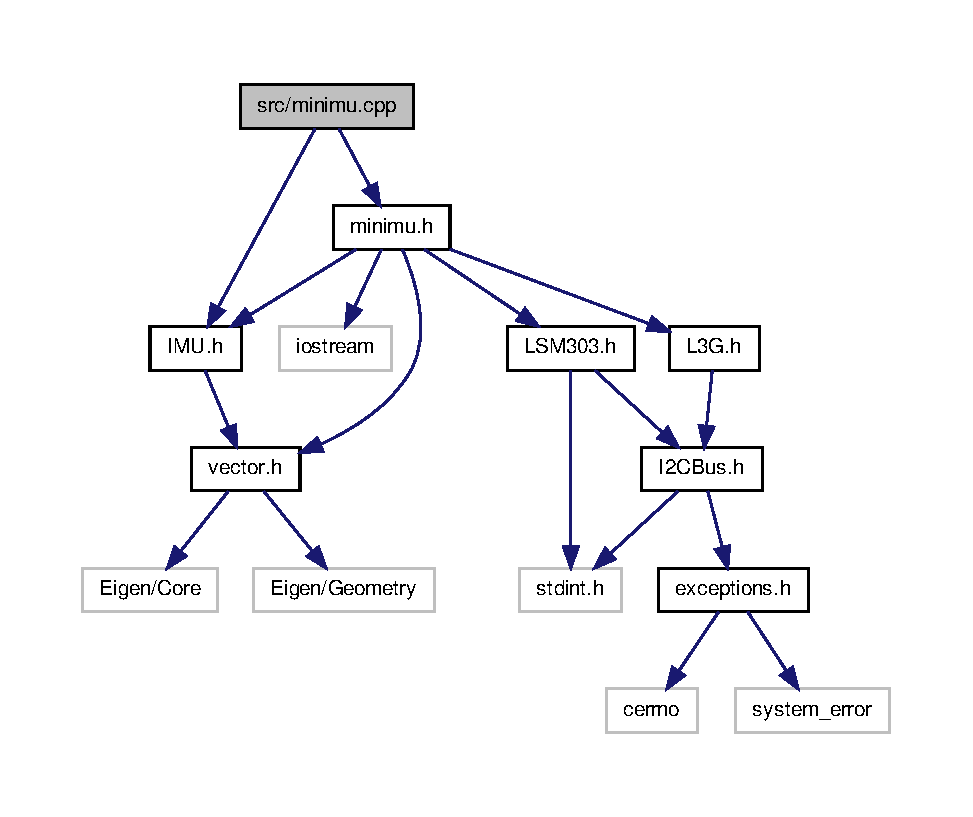
\includegraphics[width=350pt]{minimu_8cpp__incl}
\end{center}
\end{figure}

\hypertarget{minimu_8h}{\section{include/minimu.h \-File \-Reference}
\label{minimu_8h}\index{include/minimu.\-h@{include/minimu.\-h}}
}
{\ttfamily \#include \char`\"{}\-I\-M\-U.\-h\char`\"{}}\*
{\ttfamily \#include \char`\"{}\-L\-S\-M303.\-h\char`\"{}}\*
{\ttfamily \#include \char`\"{}\-L3\-G.\-h\char`\"{}}\*
{\ttfamily \#include \char`\"{}vector.\-h\char`\"{}}\*
\-Include dependency graph for minimu.\-h\-:\nopagebreak
\begin{figure}[H]
\begin{center}
\leavevmode
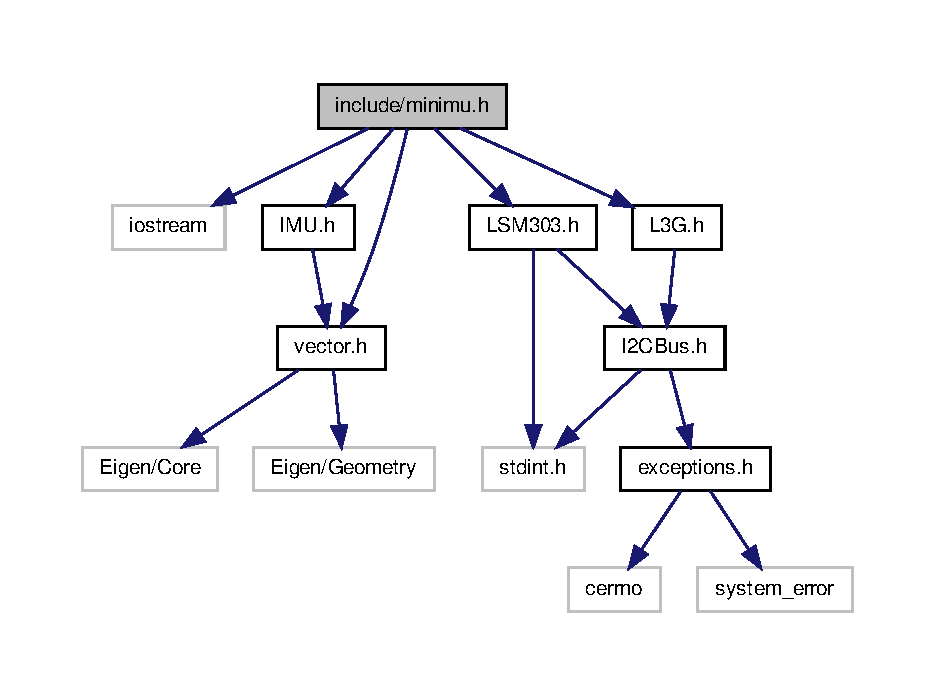
\includegraphics[width=350pt]{minimu_8h__incl}
\end{center}
\end{figure}
\-This graph shows which files directly or indirectly include this file\-:\nopagebreak
\begin{figure}[H]
\begin{center}
\leavevmode
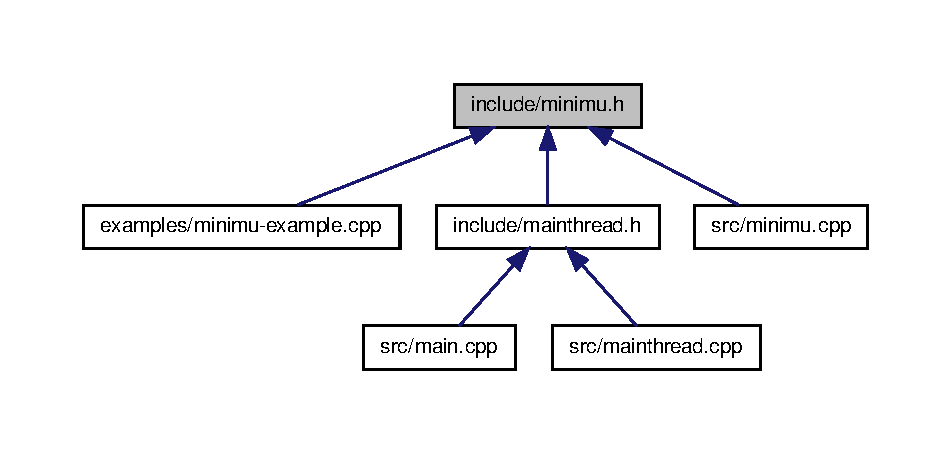
\includegraphics[width=350pt]{minimu_8h__dep__incl}
\end{center}
\end{figure}
\subsection*{\-Classes}
\begin{DoxyCompactItemize}
\item 
class \hyperlink{class_u_s_u_1_1_min_imu}{\-U\-S\-U\-::\-Min\-Imu}
\begin{DoxyCompactList}\small\item\em \-Class to manage the communication to the \-Pololu \-Min\-I\-M\-U9. \end{DoxyCompactList}\end{DoxyCompactItemize}
\subsection*{\-Namespaces}
\begin{DoxyCompactItemize}
\item 
namespace \hyperlink{namespace_u_s_u}{\-U\-S\-U}
\begin{DoxyCompactList}\small\item\em \-T\-O\-D\-O\-: \-Make some proper exceptions. \end{DoxyCompactList}\end{DoxyCompactItemize}


\subsection{\-Detailed \-Description}
\-C++ \-Min\-I\-M\-U9v2.

\begin{DoxyAuthor}{\-Author}
\-Jan \-Sommer \-Created on\-: \-Apr 20, 2013 
\end{DoxyAuthor}


\-Definition in file \hyperlink{minimu_8h_source}{minimu.\-h}.


\hypertarget{vector_8h}{\section{include/vector.h \-File \-Reference}
\label{vector_8h}\index{include/vector.\-h@{include/vector.\-h}}
}
{\ttfamily \#include \char`\"{}\-Eigen/\-Core\char`\"{}}\*
{\ttfamily \#include \char`\"{}\-Eigen/\-Geometry\char`\"{}}\*
\-Include dependency graph for vector.\-h\-:\nopagebreak
\begin{figure}[H]
\begin{center}
\leavevmode
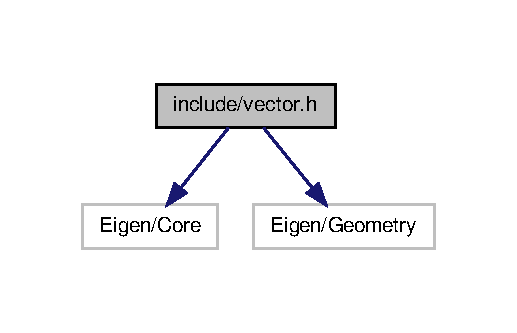
\includegraphics[width=248pt]{vector_8h__incl}
\end{center}
\end{figure}
\-This graph shows which files directly or indirectly include this file\-:\nopagebreak
\begin{figure}[H]
\begin{center}
\leavevmode
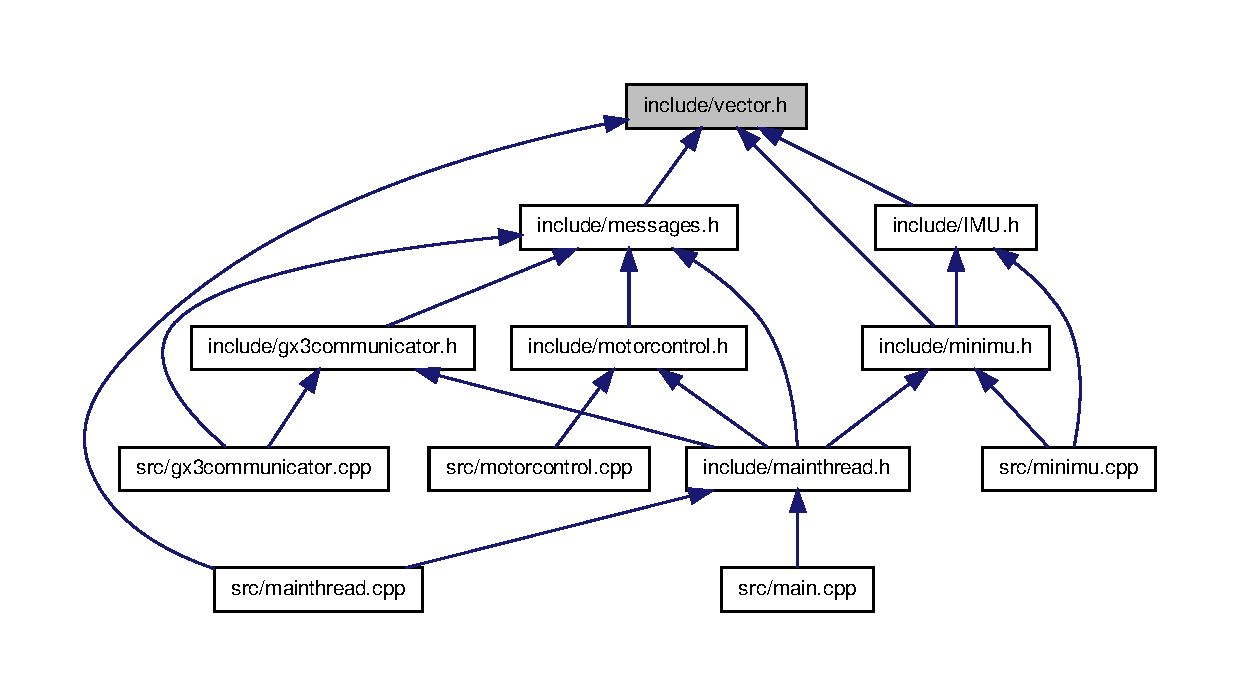
\includegraphics[width=350pt]{vector_8h__dep__incl}
\end{center}
\end{figure}
\subsection*{\-Typedefs}
\begin{DoxyCompactItemize}
\item 
typedef \-Eigen\-::\-Vector3f \hyperlink{vector_8h_a148efcf3c5319dd8961dbf9f4b846a98}{vector}
\item 
typedef \-Eigen\-::\-Vector3i \hyperlink{vector_8h_ab7556a9a18d16f7b329e566620871c95}{int\-\_\-vector}
\item 
typedef \-Eigen\-::\-Matrix3f \hyperlink{vector_8h_add320e92fcc5ba96e175a4d58d1285da}{matrix}
\item 
typedef \-Eigen\-::\-Quaternionf \hyperlink{vector_8h_afbdd744ea0fa8950d5fb4e5f68bd43b2}{quaternion}
\end{DoxyCompactItemize}


\subsection{\-Typedef \-Documentation}
\hypertarget{vector_8h_ab7556a9a18d16f7b329e566620871c95}{\index{vector.\-h@{vector.\-h}!int\-\_\-vector@{int\-\_\-vector}}
\index{int\-\_\-vector@{int\-\_\-vector}!vector.h@{vector.\-h}}
\subsubsection[{int\-\_\-vector}]{\setlength{\rightskip}{0pt plus 5cm}typedef \-Eigen\-::\-Vector3i {\bf int\-\_\-vector}}}\label{vector_8h_ab7556a9a18d16f7b329e566620871c95}


\-Definition at line 7 of file vector.\-h.

\hypertarget{vector_8h_add320e92fcc5ba96e175a4d58d1285da}{\index{vector.\-h@{vector.\-h}!matrix@{matrix}}
\index{matrix@{matrix}!vector.h@{vector.\-h}}
\subsubsection[{matrix}]{\setlength{\rightskip}{0pt plus 5cm}typedef \-Eigen\-::\-Matrix3f {\bf matrix}}}\label{vector_8h_add320e92fcc5ba96e175a4d58d1285da}


\-Definition at line 8 of file vector.\-h.

\hypertarget{vector_8h_afbdd744ea0fa8950d5fb4e5f68bd43b2}{\index{vector.\-h@{vector.\-h}!quaternion@{quaternion}}
\index{quaternion@{quaternion}!vector.h@{vector.\-h}}
\subsubsection[{quaternion}]{\setlength{\rightskip}{0pt plus 5cm}typedef \-Eigen\-::\-Quaternionf {\bf quaternion}}}\label{vector_8h_afbdd744ea0fa8950d5fb4e5f68bd43b2}


\-Definition at line 9 of file vector.\-h.

\hypertarget{vector_8h_a148efcf3c5319dd8961dbf9f4b846a98}{\index{vector.\-h@{vector.\-h}!vector@{vector}}
\index{vector@{vector}!vector.h@{vector.\-h}}
\subsubsection[{vector}]{\setlength{\rightskip}{0pt plus 5cm}typedef \-Eigen\-::\-Vector3f {\bf vector}}}\label{vector_8h_a148efcf3c5319dd8961dbf9f4b846a98}


\-Definition at line 6 of file vector.\-h.


\hypertarget{motorcontrol_8cpp}{\section{src/motorcontrol.cpp \-File \-Reference}
\label{motorcontrol_8cpp}\index{src/motorcontrol.\-cpp@{src/motorcontrol.\-cpp}}
}
{\ttfamily \#include $<$fstream$>$}\*
{\ttfamily \#include $<$stdexcept$>$}\*
{\ttfamily \#include \char`\"{}motorcontrol.\-h\char`\"{}}\*
\-Include dependency graph for motorcontrol.\-cpp\-:\nopagebreak
\begin{figure}[H]
\begin{center}
\leavevmode
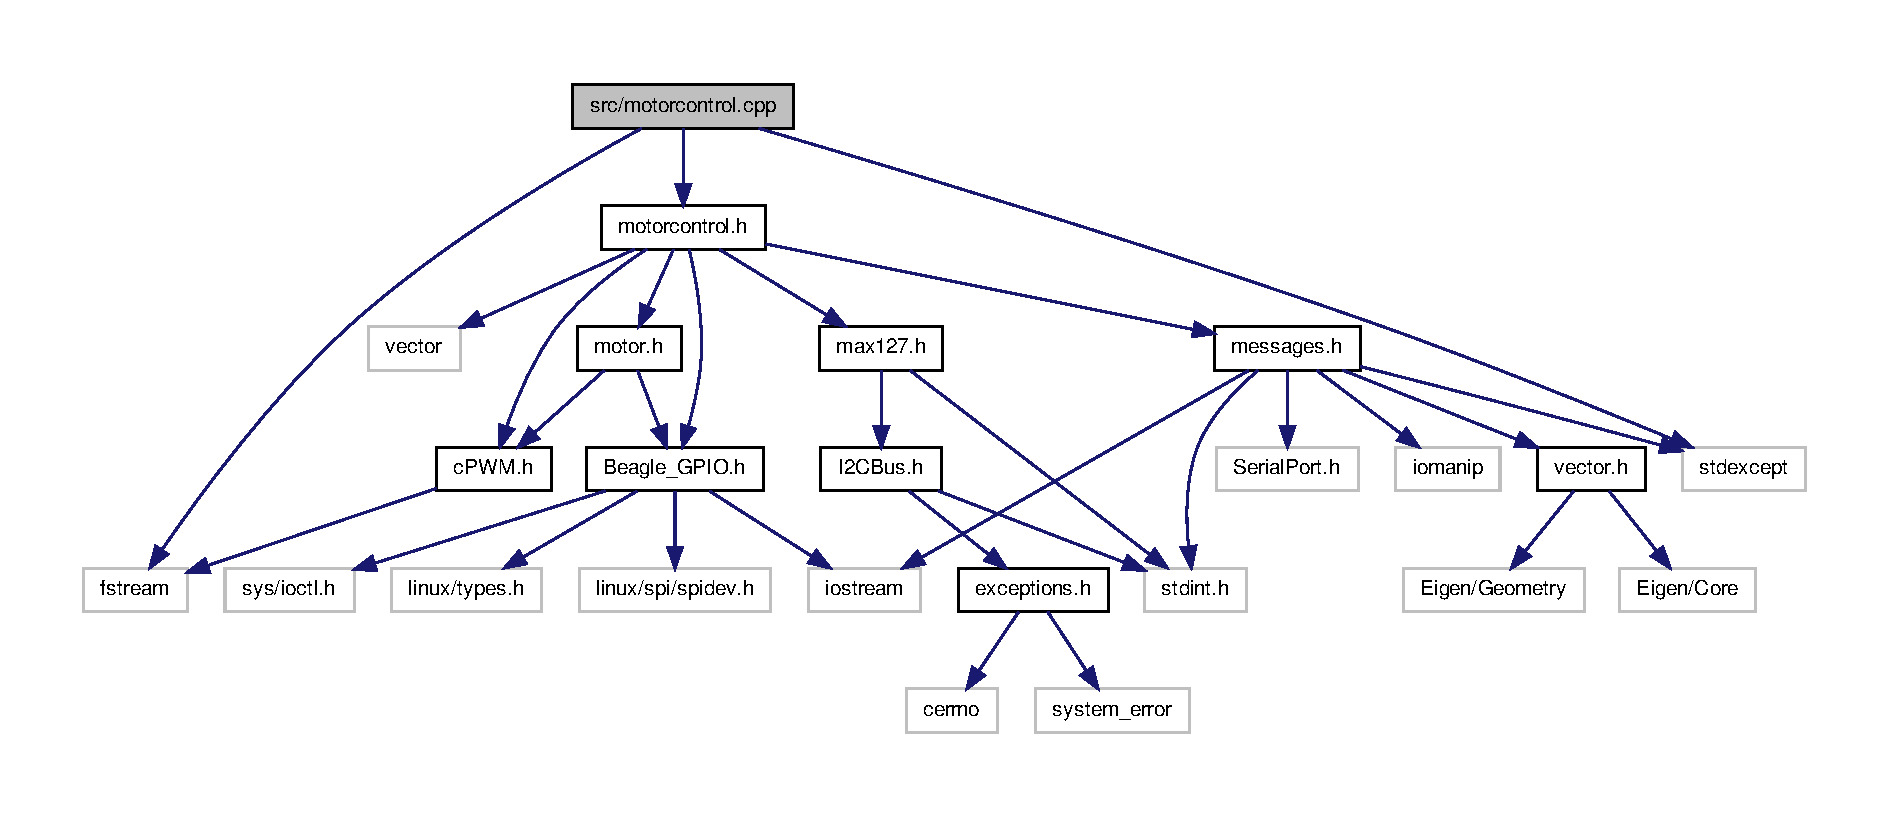
\includegraphics[width=350pt]{motorcontrol_8cpp__incl}
\end{center}
\end{figure}


\subsection{\-Detailed \-Description}
\-C++ class for the calculation of the control response. \-Based on the \-Periodic\-Rt\-Thread class.

\begin{DoxyAuthor}{\-Author}
\-Jan \-Sommer \-Created on\-: \-Apr 22, 2013 
\end{DoxyAuthor}


\-Definition in file \hyperlink{motorcontrol_8cpp_source}{motorcontrol.\-cpp}.


\hypertarget{motorcontrol_8h}{\section{motorcontrol.\-h \-File \-Reference}
\label{motorcontrol_8h}\index{motorcontrol.\-h@{motorcontrol.\-h}}
}
{\ttfamily \#include \char`\"{}threading/periodicrtthread.\-h\char`\"{}}\*
{\ttfamily \#include \char`\"{}pwm/c\-P\-W\-M.\-h\char`\"{}}\*
{\ttfamily \#include \char`\"{}pwm/\-Beagle\-\_\-\-G\-P\-I\-O.\-h\char`\"{}}\*
{\ttfamily \#include \char`\"{}pwm/motor.\-h\char`\"{}}\*
{\ttfamily \#include \char`\"{}kalmanfilter.\-h\char`\"{}}\*
\-Include dependency graph for motorcontrol.\-h\-:
\nopagebreak
\begin{figure}[H]
\begin{center}
\leavevmode
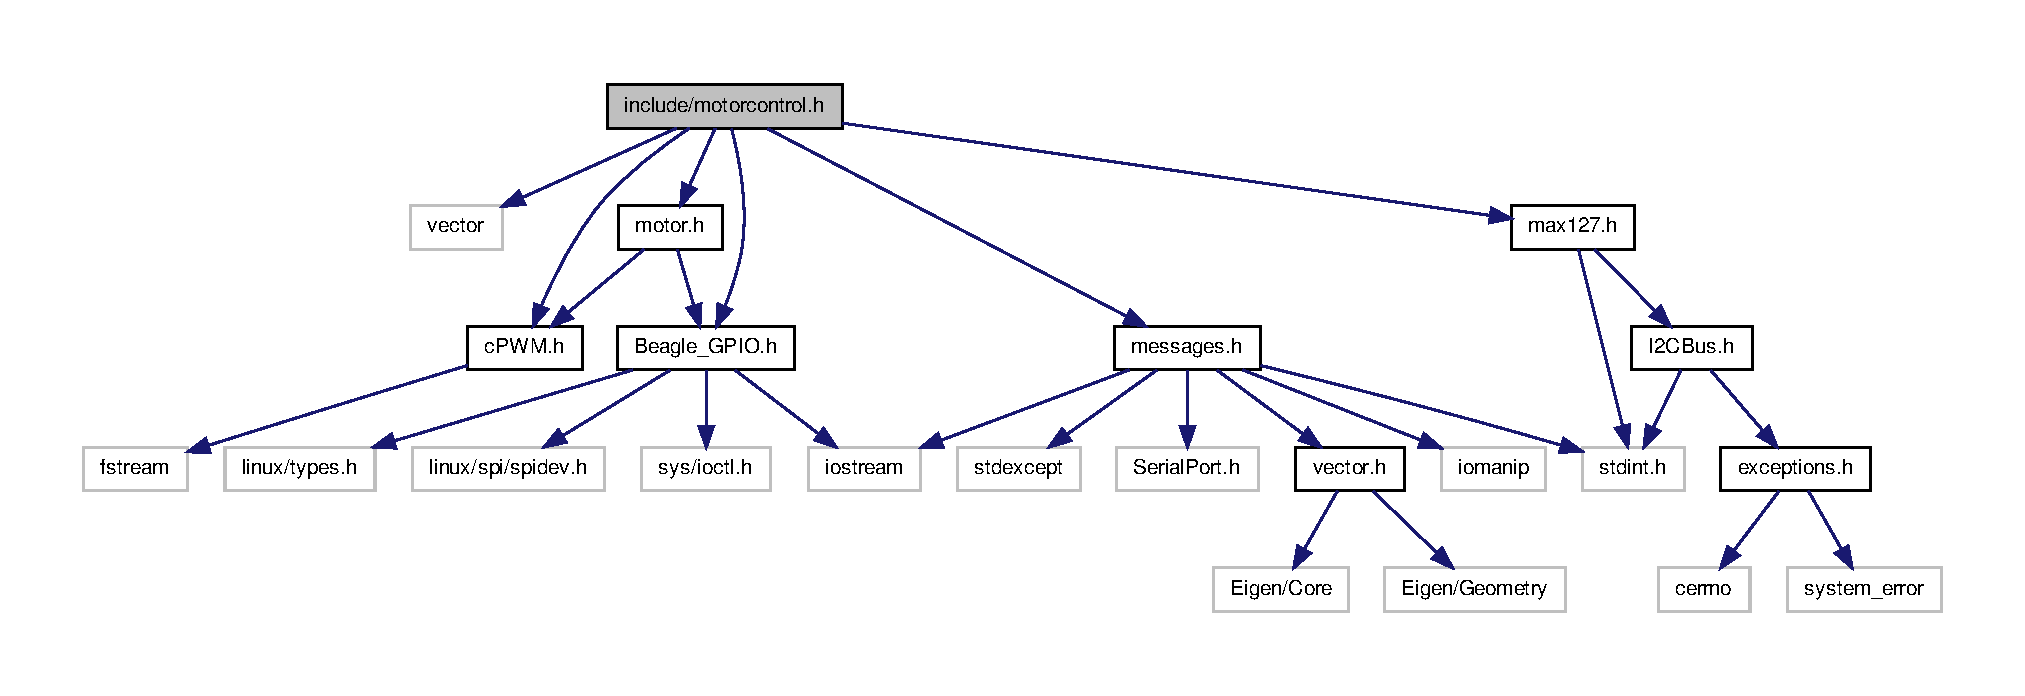
\includegraphics[width=350pt]{motorcontrol_8h__incl}
\end{center}
\end{figure}
\-This graph shows which files directly or indirectly include this file\-:\nopagebreak
\begin{figure}[H]
\begin{center}
\leavevmode
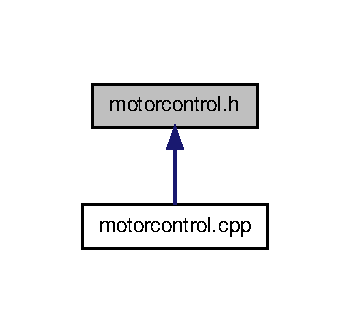
\includegraphics[width=168pt]{motorcontrol_8h__dep__incl}
\end{center}
\end{figure}
\subsection*{\-Classes}
\begin{DoxyCompactItemize}
\item 
class \hyperlink{class_u_s_u_1_1_motor_control}{\-U\-S\-U\-::\-Motor\-Control}
\begin{DoxyCompactList}\small\item\em \-Represents the \-Periodic task for motor control. \end{DoxyCompactList}\end{DoxyCompactItemize}
\subsection*{\-Namespaces}
\begin{DoxyCompactItemize}
\item 
namespace \hyperlink{namespace_u_s_u}{\-U\-S\-U}
\begin{DoxyCompactList}\small\item\em \-T\-O\-D\-O\-: \-Make some proper exceptions. \end{DoxyCompactList}\end{DoxyCompactItemize}


\subsection{\-Detailed \-Description}
\-C++ class for the calculation of the control response. \-Based on the \-Periodic\-Rt\-Thread class.

\begin{DoxyAuthor}{\-Author}
\-Jan \-Sommer \-Created on\-: \-Apr 22, 2013 
\end{DoxyAuthor}


\-Definition in file \hyperlink{motorcontrol_8h_source}{motorcontrol.\-h}.


\hypertarget{_beagle___g_p_i_o_8cpp}{\subsection{src/\-Beagle\-\_\-\-G\-P\-I\-O.cpp \-File \-Reference}
\label{_beagle___g_p_i_o_8cpp}\index{src/\-Beagle\-\_\-\-G\-P\-I\-O.\-cpp@{src/\-Beagle\-\_\-\-G\-P\-I\-O.\-cpp}}
}
{\ttfamily \#include $<$stdio.\-h$>$}\*
{\ttfamily \#include $<$stdlib.\-h$>$}\*
{\ttfamily \#include $<$sys/types.\-h$>$}\*
{\ttfamily \#include $<$sys/stat.\-h$>$}\*
{\ttfamily \#include $<$unistd.\-h$>$}\*
{\ttfamily \#include $<$fcntl.\-h$>$}\*
{\ttfamily \#include $<$sys/mman.\-h$>$}\*
{\ttfamily \#include \char`\"{}\-Beagle\-\_\-\-G\-P\-I\-O.\-h\char`\"{}}\*
\-Include dependency graph for \-Beagle\-\_\-\-G\-P\-I\-O.\-cpp\-:\nopagebreak
\begin{figure}[H]
\begin{center}
\leavevmode
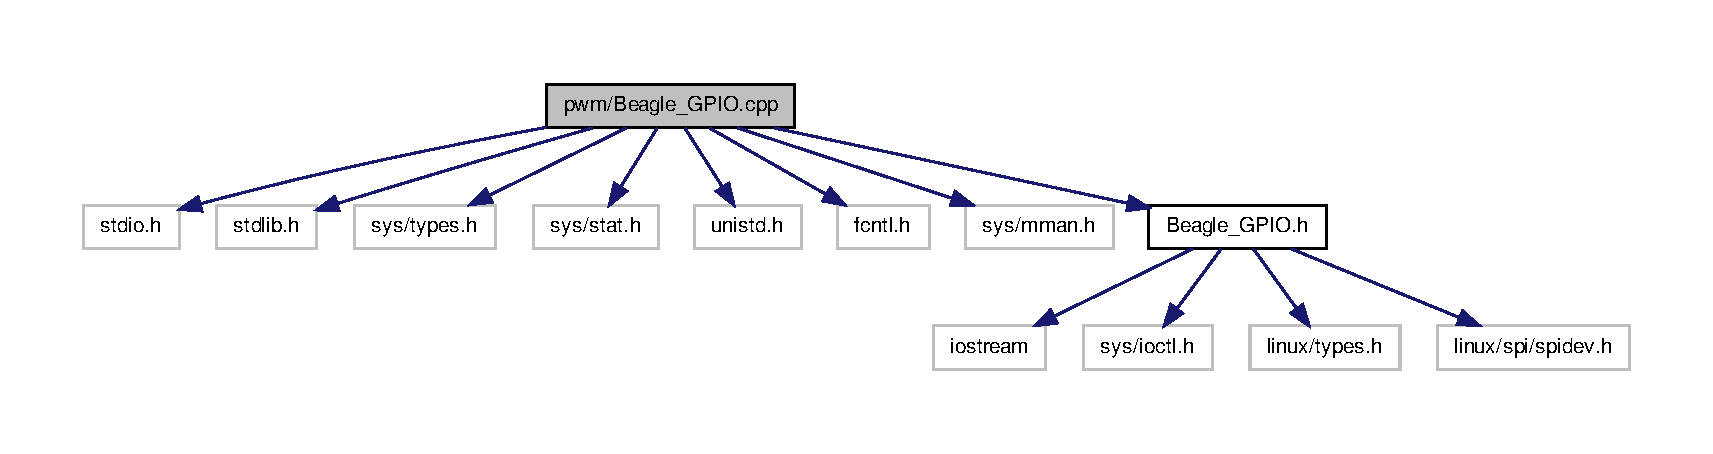
\includegraphics[width=350pt]{_beagle___g_p_i_o_8cpp__incl}
\end{center}
\end{figure}

\hypertarget{_beagle___g_p_i_o_8h}{\section{include/\-Beagle\-\_\-\-G\-P\-I\-O.h \-File \-Reference}
\label{_beagle___g_p_i_o_8h}\index{include/\-Beagle\-\_\-\-G\-P\-I\-O.\-h@{include/\-Beagle\-\_\-\-G\-P\-I\-O.\-h}}
}
{\ttfamily \#include $<$iostream$>$}\*
{\ttfamily \#include $<$sys/ioctl.\-h$>$}\*
{\ttfamily \#include $<$linux/types.\-h$>$}\*
{\ttfamily \#include $<$linux/spi/spidev.\-h$>$}\*
\-Include dependency graph for \-Beagle\-\_\-\-G\-P\-I\-O.\-h\-:\nopagebreak
\begin{figure}[H]
\begin{center}
\leavevmode
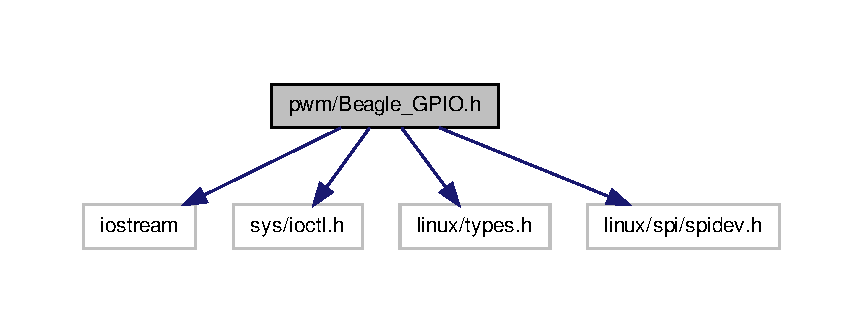
\includegraphics[width=350pt]{_beagle___g_p_i_o_8h__incl}
\end{center}
\end{figure}
\-This graph shows which files directly or indirectly include this file\-:\nopagebreak
\begin{figure}[H]
\begin{center}
\leavevmode
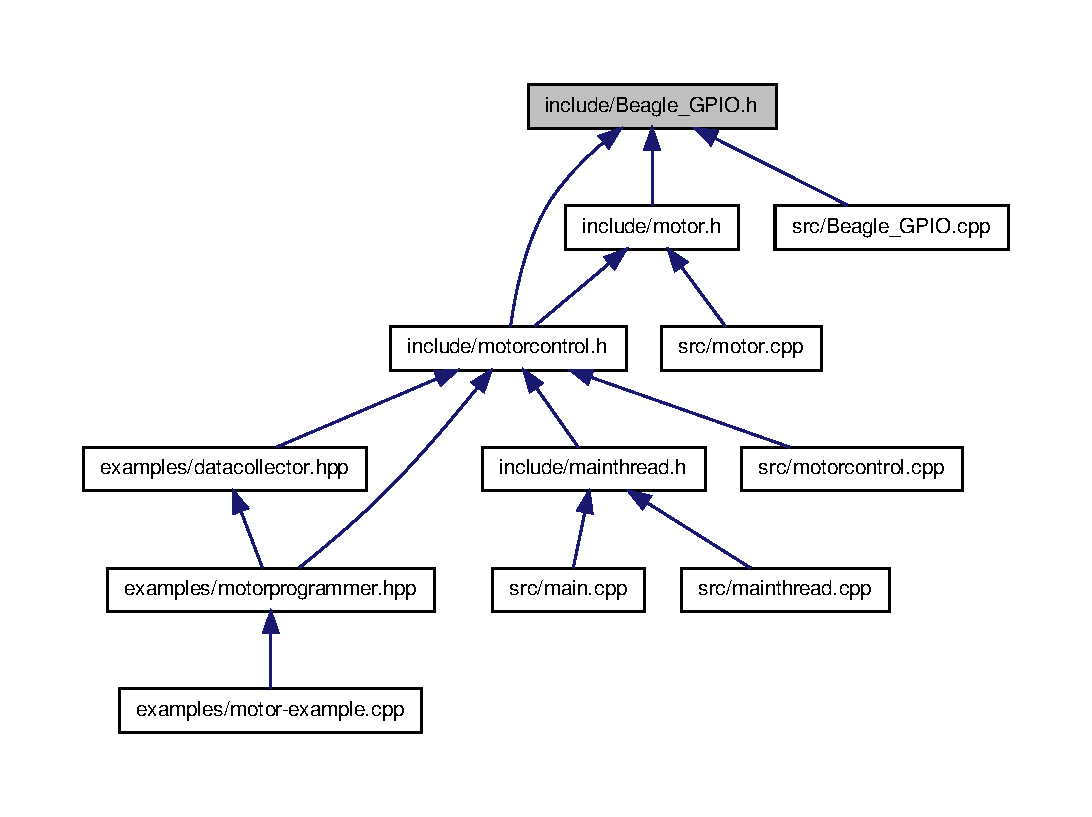
\includegraphics[width=350pt]{_beagle___g_p_i_o_8h__dep__incl}
\end{center}
\end{figure}
\subsection*{\-Classes}
\begin{DoxyCompactItemize}
\item 
class \hyperlink{class_beagle___g_p_i_o}{\-Beagle\-\_\-\-G\-P\-I\-O}
\begin{DoxyCompactList}\small\item\em \-Wrapper class to access the \-G\-P\-I\-Os of the \-Beagle\-Bone. \end{DoxyCompactList}\end{DoxyCompactItemize}
\subsection*{\-Defines}
\begin{DoxyCompactItemize}
\item 
\#define \hyperlink{_beagle___g_p_i_o_8h_a1936734e6c1d7f62fea288fdf8ca8f29}{\-G\-P\-I\-O\-\_\-\-E\-R\-R\-O\-R}(msg)~std\-::cout $<$$<$ \char`\"{}\mbox{[}\-G\-P\-I\-O\mbox{]} \-Error \-: \char`\"{} $<$$<$ msg $<$$<$ std\-::endl;
\item 
\#define \hyperlink{_beagle___g_p_i_o_8h_a4539ad479eb3f5b550fe158afba3c743}{\-B\-E\-A\-G\-L\-E\-\_\-\-G\-P\-I\-O\-\_\-\-D\-E\-B\-U\-G}
\item 
\#define \hyperlink{_beagle___g_p_i_o_8h_a3d0c439f7d891ad8c96dcd24f5407ba9}{\-G\-P\-I\-O\-\_\-\-P\-R\-I\-N\-T}(msg)~std\-::cout $<$$<$ \char`\"{}\mbox{[}\-G\-P\-I\-O\mbox{]} \-: \char`\"{} $<$$<$ msg $<$$<$ std\-::endl;
\item 
\#define \hyperlink{_beagle___g_p_i_o_8h_acdcc5aaebf3f273c1762f24a6ece2e5e}{assert}(condition)
\end{DoxyCompactItemize}


\subsection{\-Define \-Documentation}
\hypertarget{_beagle___g_p_i_o_8h_acdcc5aaebf3f273c1762f24a6ece2e5e}{\index{\-Beagle\-\_\-\-G\-P\-I\-O.\-h@{\-Beagle\-\_\-\-G\-P\-I\-O.\-h}!assert@{assert}}
\index{assert@{assert}!Beagle_GPIO.h@{\-Beagle\-\_\-\-G\-P\-I\-O.\-h}}
\subsubsection[{assert}]{\setlength{\rightskip}{0pt plus 5cm}\#define {\bf assert}(
\begin{DoxyParamCaption}
\item[{}]{condition}
\end{DoxyParamCaption}
)}}\label{_beagle___g_p_i_o_8h_acdcc5aaebf3f273c1762f24a6ece2e5e}
{\bfseries \-Value\-:}
\begin{DoxyCode}
if (!(condition))       \
                {                       \
                        GPIO_ERROR( "Assert Failed in file '" << __FILE__ << "'
       on line " << __LINE__ );        \
                        exit(0);        \
                }
\end{DoxyCode}


\-Definition at line 32 of file \-Beagle\-\_\-\-G\-P\-I\-O.\-h.

\hypertarget{_beagle___g_p_i_o_8h_a4539ad479eb3f5b550fe158afba3c743}{\index{\-Beagle\-\_\-\-G\-P\-I\-O.\-h@{\-Beagle\-\_\-\-G\-P\-I\-O.\-h}!\-B\-E\-A\-G\-L\-E\-\_\-\-G\-P\-I\-O\-\_\-\-D\-E\-B\-U\-G@{\-B\-E\-A\-G\-L\-E\-\_\-\-G\-P\-I\-O\-\_\-\-D\-E\-B\-U\-G}}
\index{\-B\-E\-A\-G\-L\-E\-\_\-\-G\-P\-I\-O\-\_\-\-D\-E\-B\-U\-G@{\-B\-E\-A\-G\-L\-E\-\_\-\-G\-P\-I\-O\-\_\-\-D\-E\-B\-U\-G}!Beagle_GPIO.h@{\-Beagle\-\_\-\-G\-P\-I\-O.\-h}}
\subsubsection[{\-B\-E\-A\-G\-L\-E\-\_\-\-G\-P\-I\-O\-\_\-\-D\-E\-B\-U\-G}]{\setlength{\rightskip}{0pt plus 5cm}\#define {\bf \-B\-E\-A\-G\-L\-E\-\_\-\-G\-P\-I\-O\-\_\-\-D\-E\-B\-U\-G}}}\label{_beagle___g_p_i_o_8h_a4539ad479eb3f5b550fe158afba3c743}


\-Definition at line 29 of file \-Beagle\-\_\-\-G\-P\-I\-O.\-h.

\hypertarget{_beagle___g_p_i_o_8h_a1936734e6c1d7f62fea288fdf8ca8f29}{\index{\-Beagle\-\_\-\-G\-P\-I\-O.\-h@{\-Beagle\-\_\-\-G\-P\-I\-O.\-h}!\-G\-P\-I\-O\-\_\-\-E\-R\-R\-O\-R@{\-G\-P\-I\-O\-\_\-\-E\-R\-R\-O\-R}}
\index{\-G\-P\-I\-O\-\_\-\-E\-R\-R\-O\-R@{\-G\-P\-I\-O\-\_\-\-E\-R\-R\-O\-R}!Beagle_GPIO.h@{\-Beagle\-\_\-\-G\-P\-I\-O.\-h}}
\subsubsection[{\-G\-P\-I\-O\-\_\-\-E\-R\-R\-O\-R}]{\setlength{\rightskip}{0pt plus 5cm}\#define {\bf \-G\-P\-I\-O\-\_\-\-E\-R\-R\-O\-R}(
\begin{DoxyParamCaption}
\item[{}]{msg}
\end{DoxyParamCaption}
)~std\-::cout $<$$<$ \char`\"{}\mbox{[}\-G\-P\-I\-O\mbox{]} \-Error \-: \char`\"{} $<$$<$ msg $<$$<$ std\-::endl;}}\label{_beagle___g_p_i_o_8h_a1936734e6c1d7f62fea288fdf8ca8f29}


\-Definition at line 27 of file \-Beagle\-\_\-\-G\-P\-I\-O.\-h.

\hypertarget{_beagle___g_p_i_o_8h_a3d0c439f7d891ad8c96dcd24f5407ba9}{\index{\-Beagle\-\_\-\-G\-P\-I\-O.\-h@{\-Beagle\-\_\-\-G\-P\-I\-O.\-h}!\-G\-P\-I\-O\-\_\-\-P\-R\-I\-N\-T@{\-G\-P\-I\-O\-\_\-\-P\-R\-I\-N\-T}}
\index{\-G\-P\-I\-O\-\_\-\-P\-R\-I\-N\-T@{\-G\-P\-I\-O\-\_\-\-P\-R\-I\-N\-T}!Beagle_GPIO.h@{\-Beagle\-\_\-\-G\-P\-I\-O.\-h}}
\subsubsection[{\-G\-P\-I\-O\-\_\-\-P\-R\-I\-N\-T}]{\setlength{\rightskip}{0pt plus 5cm}\#define {\bf \-G\-P\-I\-O\-\_\-\-P\-R\-I\-N\-T}(
\begin{DoxyParamCaption}
\item[{}]{msg}
\end{DoxyParamCaption}
)~std\-::cout $<$$<$ \char`\"{}\mbox{[}\-G\-P\-I\-O\mbox{]} \-: \char`\"{} $<$$<$ msg $<$$<$ std\-::endl;}}\label{_beagle___g_p_i_o_8h_a3d0c439f7d891ad8c96dcd24f5407ba9}


\-Definition at line 31 of file \-Beagle\-\_\-\-G\-P\-I\-O.\-h.


\hypertarget{c_p_w_m_8cpp}{\section{src/c\-P\-W\-M.cpp \-File \-Reference}
\label{c_p_w_m_8cpp}\index{src/c\-P\-W\-M.\-cpp@{src/c\-P\-W\-M.\-cpp}}
}
{\ttfamily \#include \char`\"{}c\-P\-W\-M.\-h\char`\"{}}\*
{\ttfamily \#include $<$stdexcept$>$}\*
{\ttfamily \#include $<$fstream$>$}\*
{\ttfamily \#include $<$sstream$>$}\*
\-Include dependency graph for c\-P\-W\-M.\-cpp\-:
\nopagebreak
\begin{figure}[H]
\begin{center}
\leavevmode
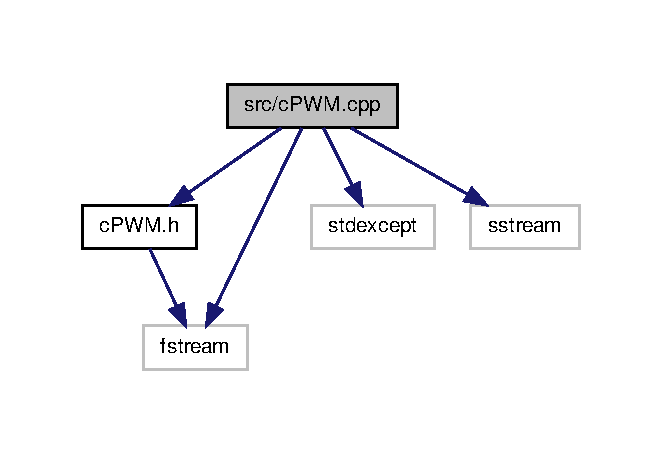
\includegraphics[width=318pt]{c_p_w_m_8cpp__incl}
\end{center}
\end{figure}


\subsection{\-Detailed \-Description}
\-Simple \-C++ class wrapper for beaglebone \-P\-W\-M e\-H\-R\-P\-W\-M interface

\begin{DoxyAuthor}{\-Author}
claus \-Created on\-: \-Jun 13, 2012 \-Author\-: claus \href{http://quadrotordiaries.blogspot.com}{\tt http\-://quadrotordiaries.\-blogspot.\-com} 
\end{DoxyAuthor}


\-Definition in file \hyperlink{c_p_w_m_8cpp_source}{c\-P\-W\-M.\-cpp}.


\hypertarget{c_p_w_m_8h}{\subsection{include/c\-P\-W\-M.h \-File \-Reference}
\label{c_p_w_m_8h}\index{include/c\-P\-W\-M.\-h@{include/c\-P\-W\-M.\-h}}
}
{\ttfamily \#include $<$fstream$>$}\*
\-Include dependency graph for c\-P\-W\-M.\-h\-:\nopagebreak
\begin{figure}[H]
\begin{center}
\leavevmode
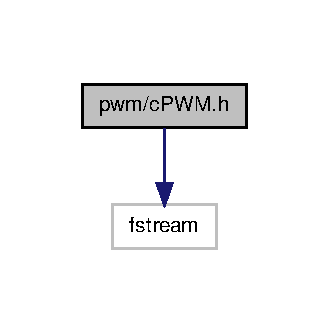
\includegraphics[width=158pt]{c_p_w_m_8h__incl}
\end{center}
\end{figure}
\-This graph shows which files directly or indirectly include this file\-:\nopagebreak
\begin{figure}[H]
\begin{center}
\leavevmode
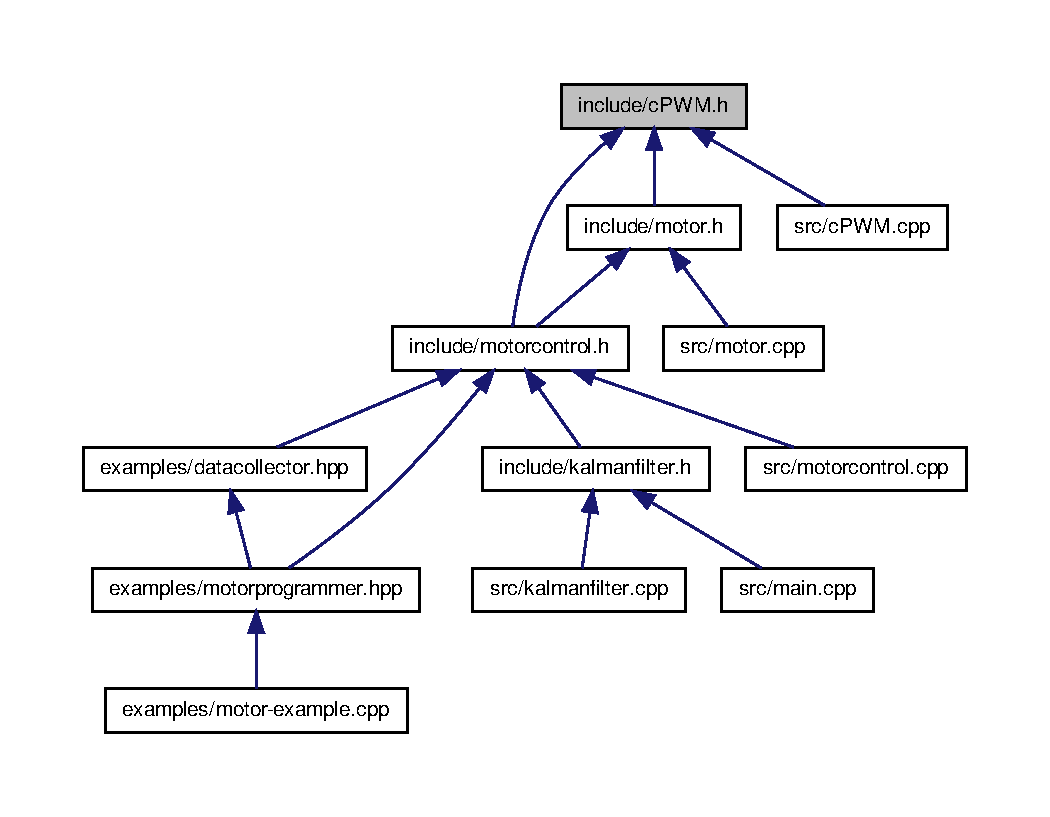
\includegraphics[width=350pt]{c_p_w_m_8h__dep__incl}
\end{center}
\end{figure}
\subsubsection*{\-Classes}
\begin{DoxyCompactItemize}
\item 
class \hyperlink{classc_p_w_m}{c\-P\-W\-M}
\begin{DoxyCompactList}\small\item\em \-Wrapper class to access the \-P\-W\-M-\/devices of the \-Beagle\-Bone. \end{DoxyCompactList}\end{DoxyCompactItemize}
\subsubsection*{\-Defines}
\begin{DoxyCompactItemize}
\item 
\#define \hyperlink{c_p_w_m_8h_a1ba5819c7195dec86e01a33333f73727}{\-S\-Y\-S\-F\-S\-\_\-\-E\-H\-R\-P\-W\-M\-\_\-\-P\-R\-E\-F\-I\-X}~\char`\"{}/sys/class/pwm/ehrpwm.\char`\"{}
\item 
\#define \hyperlink{c_p_w_m_8h_a77695d0078bb8734c092fea1153789b8}{\-S\-Y\-S\-F\-S\-\_\-\-E\-H\-R\-P\-W\-M\-\_\-\-S\-U\-F\-F\-I\-X\-\_\-\-A}~\char`\"{}\-:0\char`\"{}
\item 
\#define \hyperlink{c_p_w_m_8h_a7c349d0a2ba14e6a0c0d78f354939bb2}{\-S\-Y\-S\-F\-S\-\_\-\-E\-H\-R\-P\-W\-M\-\_\-\-S\-U\-F\-F\-I\-X\-\_\-\-B}~\char`\"{}\-:1\char`\"{}
\item 
\#define \hyperlink{c_p_w_m_8h_a3ae008f737a3f27bd780490363c2267a}{\-S\-Y\-S\-F\-S\-\_\-\-E\-H\-R\-P\-W\-M\-\_\-\-D\-U\-T\-Y\-\_\-\-N\-S}~\char`\"{}duty\-\_\-ns\char`\"{}
\item 
\#define \hyperlink{c_p_w_m_8h_afd2b94988d056d78a4e2c75acc7e454e}{\-S\-Y\-S\-F\-S\-\_\-\-E\-H\-R\-P\-W\-M\-\_\-\-D\-U\-T\-Y\-\_\-\-P\-E\-R\-C\-E\-N\-T}~\char`\"{}duty\-\_\-percent\char`\"{}
\item 
\#define \hyperlink{c_p_w_m_8h_add4a08ceb1db2a1062f7cedfaf73cc6d}{\-S\-Y\-S\-F\-S\-\_\-\-E\-H\-R\-P\-W\-M\-\_\-\-P\-E\-R\-I\-O\-D\-\_\-\-N\-S}~\char`\"{}period\-\_\-ns\char`\"{}
\item 
\#define \hyperlink{c_p_w_m_8h_ad5ab3e891281e210991cb39cdcc24cc9}{\-S\-Y\-S\-F\-S\-\_\-\-E\-H\-R\-P\-W\-M\-\_\-\-P\-E\-R\-I\-O\-D\-\_\-\-F\-R\-E\-Q}~\char`\"{}period\-\_\-freq\char`\"{}
\item 
\#define \hyperlink{c_p_w_m_8h_aab1aacedee5d8dce03422d0f09639f88}{\-S\-Y\-S\-F\-S\-\_\-\-E\-H\-R\-P\-W\-M\-\_\-\-P\-O\-L\-A\-R\-I\-T\-Y}~\char`\"{}polarity\char`\"{}
\item 
\#define \hyperlink{c_p_w_m_8h_a06034030a73c0ad8350269c15651b0fa}{\-S\-Y\-S\-F\-S\-\_\-\-E\-H\-R\-P\-W\-M\-\_\-\-R\-U\-N}~\char`\"{}run\char`\"{}
\item 
\#define \hyperlink{c_p_w_m_8h_a1aaf5e488c97bc29107020383b0a0cac}{\-S\-Y\-S\-F\-S\-\_\-\-E\-H\-R\-P\-W\-M\-\_\-\-R\-E\-Q\-U\-E\-S\-T}~\char`\"{}request\char`\"{}
\end{DoxyCompactItemize}


\subsubsection{\-Detailed \-Description}
\-Simple \-C++ class wrapper for beaglebone \-P\-W\-M e\-H\-R\-P\-W\-M interface header file

\begin{DoxyAuthor}{\-Author}
claus \-Created on\-: \-Jun 13, 2012 \-Author\-: claus \href{http://quadrotordiaries.blogspot.com}{\tt http\-://quadrotordiaries.\-blogspot.\-com} 
\end{DoxyAuthor}


\-Definition in file \hyperlink{c_p_w_m_8h_source}{c\-P\-W\-M.\-h}.



\subsubsection{\-Define \-Documentation}
\hypertarget{c_p_w_m_8h_a3ae008f737a3f27bd780490363c2267a}{\index{c\-P\-W\-M.\-h@{c\-P\-W\-M.\-h}!\-S\-Y\-S\-F\-S\-\_\-\-E\-H\-R\-P\-W\-M\-\_\-\-D\-U\-T\-Y\-\_\-\-N\-S@{\-S\-Y\-S\-F\-S\-\_\-\-E\-H\-R\-P\-W\-M\-\_\-\-D\-U\-T\-Y\-\_\-\-N\-S}}
\index{\-S\-Y\-S\-F\-S\-\_\-\-E\-H\-R\-P\-W\-M\-\_\-\-D\-U\-T\-Y\-\_\-\-N\-S@{\-S\-Y\-S\-F\-S\-\_\-\-E\-H\-R\-P\-W\-M\-\_\-\-D\-U\-T\-Y\-\_\-\-N\-S}!cPWM.h@{c\-P\-W\-M.\-h}}
\paragraph[{\-S\-Y\-S\-F\-S\-\_\-\-E\-H\-R\-P\-W\-M\-\_\-\-D\-U\-T\-Y\-\_\-\-N\-S}]{\setlength{\rightskip}{0pt plus 5cm}\#define {\bf \-S\-Y\-S\-F\-S\-\_\-\-E\-H\-R\-P\-W\-M\-\_\-\-D\-U\-T\-Y\-\_\-\-N\-S}~\char`\"{}duty\-\_\-ns\char`\"{}}}\label{c_p_w_m_8h_a3ae008f737a3f27bd780490363c2267a}


\-Definition at line \hyperlink{c_p_w_m_8h_source_l00067}{67} of file \hyperlink{c_p_w_m_8h_source}{c\-P\-W\-M.\-h}.

\hypertarget{c_p_w_m_8h_afd2b94988d056d78a4e2c75acc7e454e}{\index{c\-P\-W\-M.\-h@{c\-P\-W\-M.\-h}!\-S\-Y\-S\-F\-S\-\_\-\-E\-H\-R\-P\-W\-M\-\_\-\-D\-U\-T\-Y\-\_\-\-P\-E\-R\-C\-E\-N\-T@{\-S\-Y\-S\-F\-S\-\_\-\-E\-H\-R\-P\-W\-M\-\_\-\-D\-U\-T\-Y\-\_\-\-P\-E\-R\-C\-E\-N\-T}}
\index{\-S\-Y\-S\-F\-S\-\_\-\-E\-H\-R\-P\-W\-M\-\_\-\-D\-U\-T\-Y\-\_\-\-P\-E\-R\-C\-E\-N\-T@{\-S\-Y\-S\-F\-S\-\_\-\-E\-H\-R\-P\-W\-M\-\_\-\-D\-U\-T\-Y\-\_\-\-P\-E\-R\-C\-E\-N\-T}!cPWM.h@{c\-P\-W\-M.\-h}}
\paragraph[{\-S\-Y\-S\-F\-S\-\_\-\-E\-H\-R\-P\-W\-M\-\_\-\-D\-U\-T\-Y\-\_\-\-P\-E\-R\-C\-E\-N\-T}]{\setlength{\rightskip}{0pt plus 5cm}\#define {\bf \-S\-Y\-S\-F\-S\-\_\-\-E\-H\-R\-P\-W\-M\-\_\-\-D\-U\-T\-Y\-\_\-\-P\-E\-R\-C\-E\-N\-T}~\char`\"{}duty\-\_\-percent\char`\"{}}}\label{c_p_w_m_8h_afd2b94988d056d78a4e2c75acc7e454e}


\-Definition at line \hyperlink{c_p_w_m_8h_source_l00068}{68} of file \hyperlink{c_p_w_m_8h_source}{c\-P\-W\-M.\-h}.

\hypertarget{c_p_w_m_8h_ad5ab3e891281e210991cb39cdcc24cc9}{\index{c\-P\-W\-M.\-h@{c\-P\-W\-M.\-h}!\-S\-Y\-S\-F\-S\-\_\-\-E\-H\-R\-P\-W\-M\-\_\-\-P\-E\-R\-I\-O\-D\-\_\-\-F\-R\-E\-Q@{\-S\-Y\-S\-F\-S\-\_\-\-E\-H\-R\-P\-W\-M\-\_\-\-P\-E\-R\-I\-O\-D\-\_\-\-F\-R\-E\-Q}}
\index{\-S\-Y\-S\-F\-S\-\_\-\-E\-H\-R\-P\-W\-M\-\_\-\-P\-E\-R\-I\-O\-D\-\_\-\-F\-R\-E\-Q@{\-S\-Y\-S\-F\-S\-\_\-\-E\-H\-R\-P\-W\-M\-\_\-\-P\-E\-R\-I\-O\-D\-\_\-\-F\-R\-E\-Q}!cPWM.h@{c\-P\-W\-M.\-h}}
\paragraph[{\-S\-Y\-S\-F\-S\-\_\-\-E\-H\-R\-P\-W\-M\-\_\-\-P\-E\-R\-I\-O\-D\-\_\-\-F\-R\-E\-Q}]{\setlength{\rightskip}{0pt plus 5cm}\#define {\bf \-S\-Y\-S\-F\-S\-\_\-\-E\-H\-R\-P\-W\-M\-\_\-\-P\-E\-R\-I\-O\-D\-\_\-\-F\-R\-E\-Q}~\char`\"{}period\-\_\-freq\char`\"{}}}\label{c_p_w_m_8h_ad5ab3e891281e210991cb39cdcc24cc9}


\-Definition at line \hyperlink{c_p_w_m_8h_source_l00070}{70} of file \hyperlink{c_p_w_m_8h_source}{c\-P\-W\-M.\-h}.

\hypertarget{c_p_w_m_8h_add4a08ceb1db2a1062f7cedfaf73cc6d}{\index{c\-P\-W\-M.\-h@{c\-P\-W\-M.\-h}!\-S\-Y\-S\-F\-S\-\_\-\-E\-H\-R\-P\-W\-M\-\_\-\-P\-E\-R\-I\-O\-D\-\_\-\-N\-S@{\-S\-Y\-S\-F\-S\-\_\-\-E\-H\-R\-P\-W\-M\-\_\-\-P\-E\-R\-I\-O\-D\-\_\-\-N\-S}}
\index{\-S\-Y\-S\-F\-S\-\_\-\-E\-H\-R\-P\-W\-M\-\_\-\-P\-E\-R\-I\-O\-D\-\_\-\-N\-S@{\-S\-Y\-S\-F\-S\-\_\-\-E\-H\-R\-P\-W\-M\-\_\-\-P\-E\-R\-I\-O\-D\-\_\-\-N\-S}!cPWM.h@{c\-P\-W\-M.\-h}}
\paragraph[{\-S\-Y\-S\-F\-S\-\_\-\-E\-H\-R\-P\-W\-M\-\_\-\-P\-E\-R\-I\-O\-D\-\_\-\-N\-S}]{\setlength{\rightskip}{0pt plus 5cm}\#define {\bf \-S\-Y\-S\-F\-S\-\_\-\-E\-H\-R\-P\-W\-M\-\_\-\-P\-E\-R\-I\-O\-D\-\_\-\-N\-S}~\char`\"{}period\-\_\-ns\char`\"{}}}\label{c_p_w_m_8h_add4a08ceb1db2a1062f7cedfaf73cc6d}


\-Definition at line \hyperlink{c_p_w_m_8h_source_l00069}{69} of file \hyperlink{c_p_w_m_8h_source}{c\-P\-W\-M.\-h}.

\hypertarget{c_p_w_m_8h_aab1aacedee5d8dce03422d0f09639f88}{\index{c\-P\-W\-M.\-h@{c\-P\-W\-M.\-h}!\-S\-Y\-S\-F\-S\-\_\-\-E\-H\-R\-P\-W\-M\-\_\-\-P\-O\-L\-A\-R\-I\-T\-Y@{\-S\-Y\-S\-F\-S\-\_\-\-E\-H\-R\-P\-W\-M\-\_\-\-P\-O\-L\-A\-R\-I\-T\-Y}}
\index{\-S\-Y\-S\-F\-S\-\_\-\-E\-H\-R\-P\-W\-M\-\_\-\-P\-O\-L\-A\-R\-I\-T\-Y@{\-S\-Y\-S\-F\-S\-\_\-\-E\-H\-R\-P\-W\-M\-\_\-\-P\-O\-L\-A\-R\-I\-T\-Y}!cPWM.h@{c\-P\-W\-M.\-h}}
\paragraph[{\-S\-Y\-S\-F\-S\-\_\-\-E\-H\-R\-P\-W\-M\-\_\-\-P\-O\-L\-A\-R\-I\-T\-Y}]{\setlength{\rightskip}{0pt plus 5cm}\#define {\bf \-S\-Y\-S\-F\-S\-\_\-\-E\-H\-R\-P\-W\-M\-\_\-\-P\-O\-L\-A\-R\-I\-T\-Y}~\char`\"{}polarity\char`\"{}}}\label{c_p_w_m_8h_aab1aacedee5d8dce03422d0f09639f88}


\-Definition at line \hyperlink{c_p_w_m_8h_source_l00071}{71} of file \hyperlink{c_p_w_m_8h_source}{c\-P\-W\-M.\-h}.

\hypertarget{c_p_w_m_8h_a1ba5819c7195dec86e01a33333f73727}{\index{c\-P\-W\-M.\-h@{c\-P\-W\-M.\-h}!\-S\-Y\-S\-F\-S\-\_\-\-E\-H\-R\-P\-W\-M\-\_\-\-P\-R\-E\-F\-I\-X@{\-S\-Y\-S\-F\-S\-\_\-\-E\-H\-R\-P\-W\-M\-\_\-\-P\-R\-E\-F\-I\-X}}
\index{\-S\-Y\-S\-F\-S\-\_\-\-E\-H\-R\-P\-W\-M\-\_\-\-P\-R\-E\-F\-I\-X@{\-S\-Y\-S\-F\-S\-\_\-\-E\-H\-R\-P\-W\-M\-\_\-\-P\-R\-E\-F\-I\-X}!cPWM.h@{c\-P\-W\-M.\-h}}
\paragraph[{\-S\-Y\-S\-F\-S\-\_\-\-E\-H\-R\-P\-W\-M\-\_\-\-P\-R\-E\-F\-I\-X}]{\setlength{\rightskip}{0pt plus 5cm}\#define {\bf \-S\-Y\-S\-F\-S\-\_\-\-E\-H\-R\-P\-W\-M\-\_\-\-P\-R\-E\-F\-I\-X}~\char`\"{}/sys/class/pwm/ehrpwm.\char`\"{}}}\label{c_p_w_m_8h_a1ba5819c7195dec86e01a33333f73727}


\-Definition at line \hyperlink{c_p_w_m_8h_source_l00064}{64} of file \hyperlink{c_p_w_m_8h_source}{c\-P\-W\-M.\-h}.

\hypertarget{c_p_w_m_8h_a1aaf5e488c97bc29107020383b0a0cac}{\index{c\-P\-W\-M.\-h@{c\-P\-W\-M.\-h}!\-S\-Y\-S\-F\-S\-\_\-\-E\-H\-R\-P\-W\-M\-\_\-\-R\-E\-Q\-U\-E\-S\-T@{\-S\-Y\-S\-F\-S\-\_\-\-E\-H\-R\-P\-W\-M\-\_\-\-R\-E\-Q\-U\-E\-S\-T}}
\index{\-S\-Y\-S\-F\-S\-\_\-\-E\-H\-R\-P\-W\-M\-\_\-\-R\-E\-Q\-U\-E\-S\-T@{\-S\-Y\-S\-F\-S\-\_\-\-E\-H\-R\-P\-W\-M\-\_\-\-R\-E\-Q\-U\-E\-S\-T}!cPWM.h@{c\-P\-W\-M.\-h}}
\paragraph[{\-S\-Y\-S\-F\-S\-\_\-\-E\-H\-R\-P\-W\-M\-\_\-\-R\-E\-Q\-U\-E\-S\-T}]{\setlength{\rightskip}{0pt plus 5cm}\#define {\bf \-S\-Y\-S\-F\-S\-\_\-\-E\-H\-R\-P\-W\-M\-\_\-\-R\-E\-Q\-U\-E\-S\-T}~\char`\"{}request\char`\"{}}}\label{c_p_w_m_8h_a1aaf5e488c97bc29107020383b0a0cac}


\-Definition at line \hyperlink{c_p_w_m_8h_source_l00073}{73} of file \hyperlink{c_p_w_m_8h_source}{c\-P\-W\-M.\-h}.

\hypertarget{c_p_w_m_8h_a06034030a73c0ad8350269c15651b0fa}{\index{c\-P\-W\-M.\-h@{c\-P\-W\-M.\-h}!\-S\-Y\-S\-F\-S\-\_\-\-E\-H\-R\-P\-W\-M\-\_\-\-R\-U\-N@{\-S\-Y\-S\-F\-S\-\_\-\-E\-H\-R\-P\-W\-M\-\_\-\-R\-U\-N}}
\index{\-S\-Y\-S\-F\-S\-\_\-\-E\-H\-R\-P\-W\-M\-\_\-\-R\-U\-N@{\-S\-Y\-S\-F\-S\-\_\-\-E\-H\-R\-P\-W\-M\-\_\-\-R\-U\-N}!cPWM.h@{c\-P\-W\-M.\-h}}
\paragraph[{\-S\-Y\-S\-F\-S\-\_\-\-E\-H\-R\-P\-W\-M\-\_\-\-R\-U\-N}]{\setlength{\rightskip}{0pt plus 5cm}\#define {\bf \-S\-Y\-S\-F\-S\-\_\-\-E\-H\-R\-P\-W\-M\-\_\-\-R\-U\-N}~\char`\"{}run\char`\"{}}}\label{c_p_w_m_8h_a06034030a73c0ad8350269c15651b0fa}


\-Definition at line \hyperlink{c_p_w_m_8h_source_l00072}{72} of file \hyperlink{c_p_w_m_8h_source}{c\-P\-W\-M.\-h}.

\hypertarget{c_p_w_m_8h_a77695d0078bb8734c092fea1153789b8}{\index{c\-P\-W\-M.\-h@{c\-P\-W\-M.\-h}!\-S\-Y\-S\-F\-S\-\_\-\-E\-H\-R\-P\-W\-M\-\_\-\-S\-U\-F\-F\-I\-X\-\_\-\-A@{\-S\-Y\-S\-F\-S\-\_\-\-E\-H\-R\-P\-W\-M\-\_\-\-S\-U\-F\-F\-I\-X\-\_\-\-A}}
\index{\-S\-Y\-S\-F\-S\-\_\-\-E\-H\-R\-P\-W\-M\-\_\-\-S\-U\-F\-F\-I\-X\-\_\-\-A@{\-S\-Y\-S\-F\-S\-\_\-\-E\-H\-R\-P\-W\-M\-\_\-\-S\-U\-F\-F\-I\-X\-\_\-\-A}!cPWM.h@{c\-P\-W\-M.\-h}}
\paragraph[{\-S\-Y\-S\-F\-S\-\_\-\-E\-H\-R\-P\-W\-M\-\_\-\-S\-U\-F\-F\-I\-X\-\_\-\-A}]{\setlength{\rightskip}{0pt plus 5cm}\#define {\bf \-S\-Y\-S\-F\-S\-\_\-\-E\-H\-R\-P\-W\-M\-\_\-\-S\-U\-F\-F\-I\-X\-\_\-\-A}~\char`\"{}\-:0\char`\"{}}}\label{c_p_w_m_8h_a77695d0078bb8734c092fea1153789b8}


\-Definition at line \hyperlink{c_p_w_m_8h_source_l00065}{65} of file \hyperlink{c_p_w_m_8h_source}{c\-P\-W\-M.\-h}.

\hypertarget{c_p_w_m_8h_a7c349d0a2ba14e6a0c0d78f354939bb2}{\index{c\-P\-W\-M.\-h@{c\-P\-W\-M.\-h}!\-S\-Y\-S\-F\-S\-\_\-\-E\-H\-R\-P\-W\-M\-\_\-\-S\-U\-F\-F\-I\-X\-\_\-\-B@{\-S\-Y\-S\-F\-S\-\_\-\-E\-H\-R\-P\-W\-M\-\_\-\-S\-U\-F\-F\-I\-X\-\_\-\-B}}
\index{\-S\-Y\-S\-F\-S\-\_\-\-E\-H\-R\-P\-W\-M\-\_\-\-S\-U\-F\-F\-I\-X\-\_\-\-B@{\-S\-Y\-S\-F\-S\-\_\-\-E\-H\-R\-P\-W\-M\-\_\-\-S\-U\-F\-F\-I\-X\-\_\-\-B}!cPWM.h@{c\-P\-W\-M.\-h}}
\paragraph[{\-S\-Y\-S\-F\-S\-\_\-\-E\-H\-R\-P\-W\-M\-\_\-\-S\-U\-F\-F\-I\-X\-\_\-\-B}]{\setlength{\rightskip}{0pt plus 5cm}\#define {\bf \-S\-Y\-S\-F\-S\-\_\-\-E\-H\-R\-P\-W\-M\-\_\-\-S\-U\-F\-F\-I\-X\-\_\-\-B}~\char`\"{}\-:1\char`\"{}}}\label{c_p_w_m_8h_a7c349d0a2ba14e6a0c0d78f354939bb2}


\-Definition at line \hyperlink{c_p_w_m_8h_source_l00066}{66} of file \hyperlink{c_p_w_m_8h_source}{c\-P\-W\-M.\-h}.


\hypertarget{motor_8cpp}{\section{pwm/motor.cpp \-File \-Reference}
\label{motor_8cpp}\index{pwm/motor.\-cpp@{pwm/motor.\-cpp}}
}
{\ttfamily \#include \char`\"{}motor.\-h\char`\"{}}\*
\-Include dependency graph for motor.\-cpp\-:\nopagebreak
\begin{figure}[H]
\begin{center}
\leavevmode
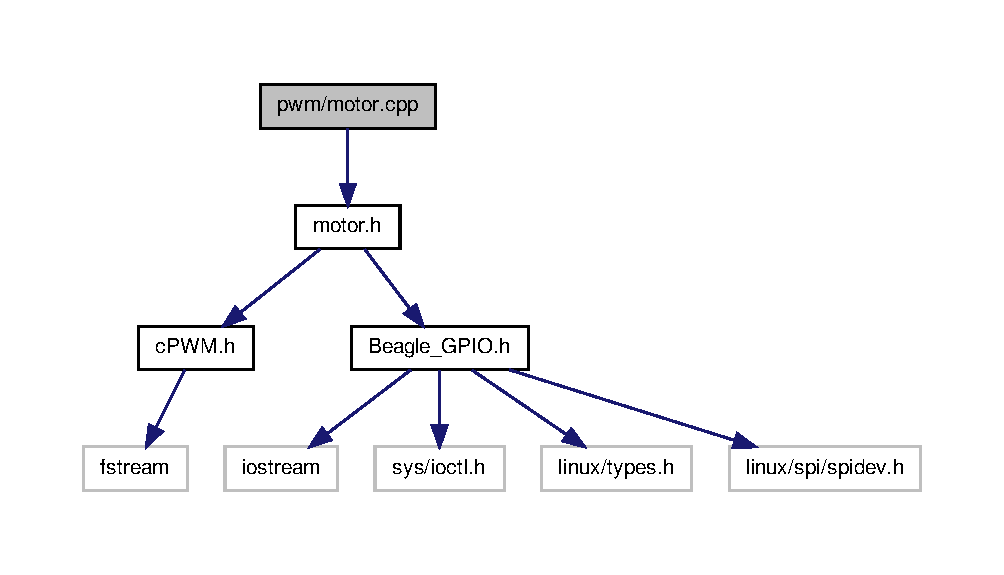
\includegraphics[width=350pt]{motor_8cpp__incl}
\end{center}
\end{figure}


\subsection{\-Detailed \-Description}
\-Class to represent a motor

\begin{DoxyAuthor}{\-Author}
\-Jan \-Sommer \-Created on\-: \-Apr 22, 2013 
\end{DoxyAuthor}


\-Definition in file \hyperlink{motor_8cpp_source}{motor.\-cpp}.


\hypertarget{motor_8h}{\subsection{include/motor.h \-File \-Reference}
\label{motor_8h}\index{include/motor.\-h@{include/motor.\-h}}
}
{\ttfamily \#include \char`\"{}c\-P\-W\-M.\-h\char`\"{}}\*
{\ttfamily \#include \char`\"{}\-Beagle\-\_\-\-G\-P\-I\-O.\-h\char`\"{}}\*
\-Include dependency graph for motor.\-h\-:\nopagebreak
\begin{figure}[H]
\begin{center}
\leavevmode
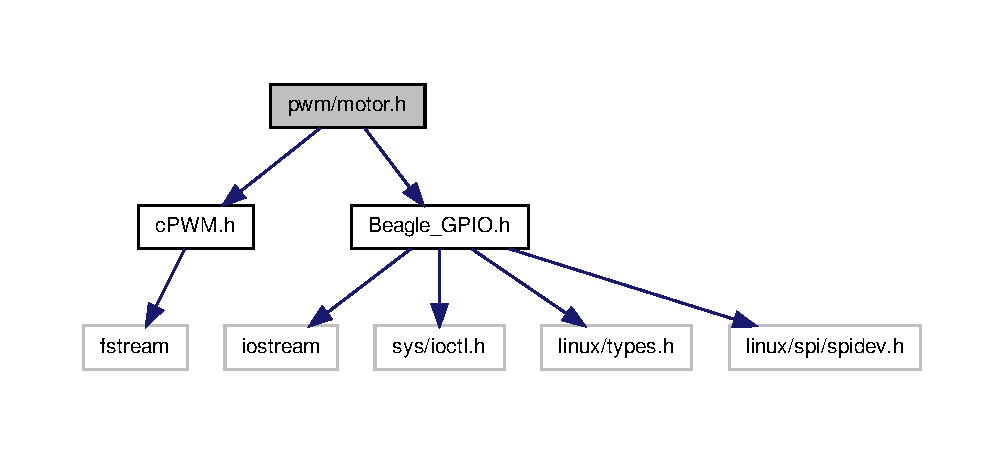
\includegraphics[width=350pt]{motor_8h__incl}
\end{center}
\end{figure}
\-This graph shows which files directly or indirectly include this file\-:\nopagebreak
\begin{figure}[H]
\begin{center}
\leavevmode
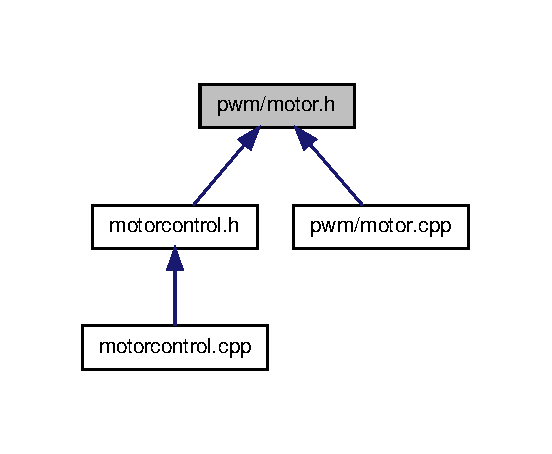
\includegraphics[width=350pt]{motor_8h__dep__incl}
\end{center}
\end{figure}
\subsubsection*{\-Classes}
\begin{DoxyCompactItemize}
\item 
class \hyperlink{class_u_s_u_1_1_motor}{\-U\-S\-U\-::\-Motor}
\begin{DoxyCompactList}\small\item\em \-Class which represents a motor. \end{DoxyCompactList}\end{DoxyCompactItemize}
\subsubsection*{\-Namespaces}
\begin{DoxyCompactItemize}
\item 
namespace \hyperlink{namespace_u_s_u}{\-U\-S\-U}
\begin{DoxyCompactList}\small\item\em \-T\-O\-D\-O\-: \-Make some proper exceptions. \end{DoxyCompactList}\end{DoxyCompactItemize}
\subsubsection*{\-Typedefs}
\begin{DoxyCompactItemize}
\item 
typedef void(c\-P\-W\-M\-::$\ast$ \hyperlink{motor_8h_aa4a2cd53d0866ae4c273573db3c4870d}{\-Set\-Duty\-Cyle} )(unsigned int)
\begin{DoxyCompactList}\small\item\em \-Function-\/pointer to the \-Set\-Duty\-Cyle-\/method of \hyperlink{classc_p_w_m}{c\-P\-W\-M} class. \end{DoxyCompactList}\end{DoxyCompactItemize}


\subsubsection{\-Detailed \-Description}
\-Class to represent a motor

\begin{DoxyAuthor}{\-Author}
\-Jan \-Sommer \-Created on\-: \-Apr 22, 2013 
\end{DoxyAuthor}


\-Definition in file \hyperlink{motor_8h_source}{motor.\-h}.



\subsubsection{\-Typedef \-Documentation}
\hypertarget{motor_8h_aa4a2cd53d0866ae4c273573db3c4870d}{\index{motor.\-h@{motor.\-h}!\-Set\-Duty\-Cyle@{\-Set\-Duty\-Cyle}}
\index{\-Set\-Duty\-Cyle@{\-Set\-Duty\-Cyle}!motor.h@{motor.\-h}}
\paragraph[{\-Set\-Duty\-Cyle}]{\setlength{\rightskip}{0pt plus 5cm}typedef void(c\-P\-W\-M\-::$\ast$ {\bf \-Set\-Duty\-Cyle})(unsigned int)}}\label{motor_8h_aa4a2cd53d0866ae4c273573db3c4870d}


\-Function-\/pointer to the \-Set\-Duty\-Cyle-\/method of \hyperlink{classc_p_w_m}{c\-P\-W\-M} class. 

\-Each \hyperlink{classc_p_w_m}{c\-P\-W\-M} object has 2 channels (\-A and \-B). \-Each motor gets assigned to one of the channels using the corresponding function pointer. 

\-Definition at line \hyperlink{motor_8h_source_l00023}{23} of file \hyperlink{motor_8h_source}{motor.\-h}.


\hypertarget{set_p_w_m_8c}{\section{pwm/set\-P\-W\-M.c \-File \-Reference}
\label{set_p_w_m_8c}\index{pwm/set\-P\-W\-M.\-c@{pwm/set\-P\-W\-M.\-c}}
}
{\ttfamily \#include $<$stdio.\-h$>$}\*
{\ttfamily \#include $<$string.\-h$>$}\*
{\ttfamily \#include $<$stdlib.\-h$>$}\*
{\ttfamily \#include $<$sys/types.\-h$>$}\*
{\ttfamily \#include $<$sys/stat.\-h$>$}\*
{\ttfamily \#include $<$fcntl.\-h$>$}\*
{\ttfamily \#include $<$stdint.\-h$>$}\*
{\ttfamily \#include $<$sys/mman.\-h$>$}\*
{\ttfamily \#include $<$unistd.\-h$>$}\*
\-Include dependency graph for set\-P\-W\-M.\-c\-:\nopagebreak
\begin{figure}[H]
\begin{center}
\leavevmode
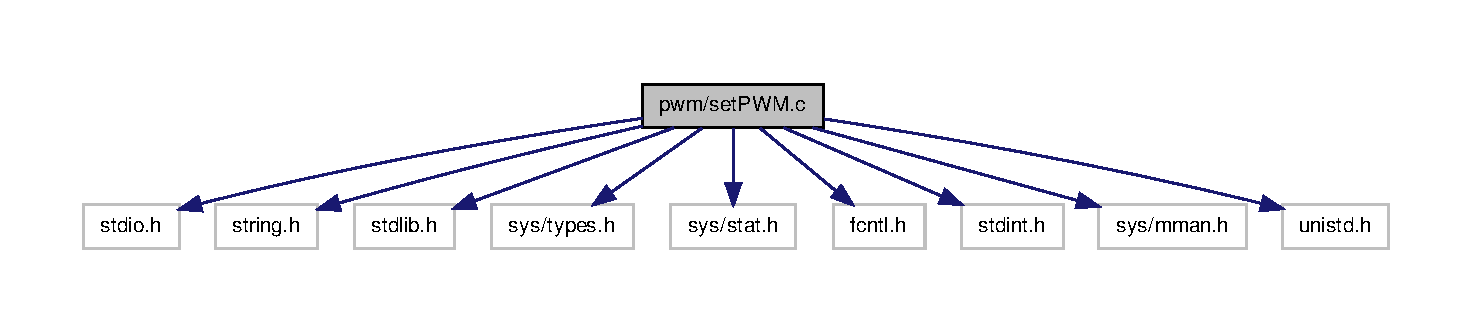
\includegraphics[width=350pt]{set_p_w_m_8c__incl}
\end{center}
\end{figure}
\subsection*{\-Defines}
\begin{DoxyCompactItemize}
\item 
\#define \hyperlink{set_p_w_m_8c_a322c03575b214dad5f9e8105017ebff4}{\-C\-M\-\_\-\-P\-E\-R\-\_\-\-R\-E\-G\-\_\-\-S\-T\-A\-R\-T}~0x44e00000
\item 
\#define \hyperlink{set_p_w_m_8c_ad99e8b7c4c7dd31ae94b872789dc05c6}{\-C\-M\-\_\-\-P\-E\-R\-\_\-\-R\-E\-G\-\_\-\-L\-E\-N\-G\-T\-H}~1024
\item 
\#define \hyperlink{set_p_w_m_8c_a7c30f10373deece9b3c4832214254f6b}{\-C\-M\-\_\-\-P\-E\-R\-\_\-\-E\-P\-W\-M\-S\-S0\-\_\-\-C\-L\-K\-C\-T\-R\-L\-\_\-\-O\-F\-F\-S\-E\-T}~0xd4
\item 
\#define \hyperlink{set_p_w_m_8c_a9a1ff71a677c19daab7a07548b594890}{\-C\-M\-\_\-\-P\-E\-R\-\_\-\-E\-P\-W\-M\-S\-S1\-\_\-\-C\-L\-K\-C\-T\-R\-L\-\_\-\-O\-F\-F\-S\-E\-T}~0xcc
\item 
\#define \hyperlink{set_p_w_m_8c_a4c44b717268ed38c31160ad166365f98}{\-C\-M\-\_\-\-P\-E\-R\-\_\-\-E\-P\-W\-M\-S\-S2\-\_\-\-C\-L\-K\-C\-T\-R\-L\-\_\-\-O\-F\-F\-S\-E\-T}~0xd8
\item 
\#define \hyperlink{set_p_w_m_8c_a1a7412a14f779cf6e360c37dd138b544}{\-P\-W\-M\-\_\-\-C\-L\-O\-C\-K\-\_\-\-E\-N\-A\-B\-L\-E}~0x2
\item 
\#define \hyperlink{set_p_w_m_8c_a1ad5533b9833271a0afe1665b2091de6}{\-P\-W\-M\-\_\-\-C\-L\-O\-C\-K\-\_\-\-D\-I\-S\-A\-B\-L\-E}~0x0
\item 
\#define \hyperlink{set_p_w_m_8c_a11821146334673886675fbb9ff645579}{\-P\-W\-M\-\_\-\-L\-I\-S\-T\-\_\-\-M\-A\-X}~3
\end{DoxyCompactItemize}
\subsection*{\-Functions}
\begin{DoxyCompactItemize}
\item 
void \hyperlink{set_p_w_m_8c_ad64a1abe6d3f1789825c8ddada15f260}{print\-\_\-usage} (const char $\ast$message)
\item 
int \hyperlink{set_p_w_m_8c_a3c04138a5bfe5d72780bb7e82a18e627}{main} (int argc, char $\ast$$\ast$argv)
\end{DoxyCompactItemize}
\subsection*{\-Variables}
\begin{DoxyCompactItemize}
\item 
int \hyperlink{set_p_w_m_8c_a5dbabbd7e1d5ecc67eb4680bf18e6b72}{\-P\-W\-M\-\_\-\-O\-F\-F\-S\-E\-T\-S} \mbox{[}\hyperlink{set_p_w_m_8c_a11821146334673886675fbb9ff645579}{\-P\-W\-M\-\_\-\-L\-I\-S\-T\-\_\-\-M\-A\-X}\mbox{]}
\end{DoxyCompactItemize}


\subsection{\-Define \-Documentation}
\hypertarget{set_p_w_m_8c_a7c30f10373deece9b3c4832214254f6b}{\index{set\-P\-W\-M.\-c@{set\-P\-W\-M.\-c}!\-C\-M\-\_\-\-P\-E\-R\-\_\-\-E\-P\-W\-M\-S\-S0\-\_\-\-C\-L\-K\-C\-T\-R\-L\-\_\-\-O\-F\-F\-S\-E\-T@{\-C\-M\-\_\-\-P\-E\-R\-\_\-\-E\-P\-W\-M\-S\-S0\-\_\-\-C\-L\-K\-C\-T\-R\-L\-\_\-\-O\-F\-F\-S\-E\-T}}
\index{\-C\-M\-\_\-\-P\-E\-R\-\_\-\-E\-P\-W\-M\-S\-S0\-\_\-\-C\-L\-K\-C\-T\-R\-L\-\_\-\-O\-F\-F\-S\-E\-T@{\-C\-M\-\_\-\-P\-E\-R\-\_\-\-E\-P\-W\-M\-S\-S0\-\_\-\-C\-L\-K\-C\-T\-R\-L\-\_\-\-O\-F\-F\-S\-E\-T}!setPWM.c@{set\-P\-W\-M.\-c}}
\subsubsection[{\-C\-M\-\_\-\-P\-E\-R\-\_\-\-E\-P\-W\-M\-S\-S0\-\_\-\-C\-L\-K\-C\-T\-R\-L\-\_\-\-O\-F\-F\-S\-E\-T}]{\setlength{\rightskip}{0pt plus 5cm}\#define {\bf \-C\-M\-\_\-\-P\-E\-R\-\_\-\-E\-P\-W\-M\-S\-S0\-\_\-\-C\-L\-K\-C\-T\-R\-L\-\_\-\-O\-F\-F\-S\-E\-T}~0xd4}}\label{set_p_w_m_8c_a7c30f10373deece9b3c4832214254f6b}


\-Definition at line 13 of file set\-P\-W\-M.\-c.

\hypertarget{set_p_w_m_8c_a9a1ff71a677c19daab7a07548b594890}{\index{set\-P\-W\-M.\-c@{set\-P\-W\-M.\-c}!\-C\-M\-\_\-\-P\-E\-R\-\_\-\-E\-P\-W\-M\-S\-S1\-\_\-\-C\-L\-K\-C\-T\-R\-L\-\_\-\-O\-F\-F\-S\-E\-T@{\-C\-M\-\_\-\-P\-E\-R\-\_\-\-E\-P\-W\-M\-S\-S1\-\_\-\-C\-L\-K\-C\-T\-R\-L\-\_\-\-O\-F\-F\-S\-E\-T}}
\index{\-C\-M\-\_\-\-P\-E\-R\-\_\-\-E\-P\-W\-M\-S\-S1\-\_\-\-C\-L\-K\-C\-T\-R\-L\-\_\-\-O\-F\-F\-S\-E\-T@{\-C\-M\-\_\-\-P\-E\-R\-\_\-\-E\-P\-W\-M\-S\-S1\-\_\-\-C\-L\-K\-C\-T\-R\-L\-\_\-\-O\-F\-F\-S\-E\-T}!setPWM.c@{set\-P\-W\-M.\-c}}
\subsubsection[{\-C\-M\-\_\-\-P\-E\-R\-\_\-\-E\-P\-W\-M\-S\-S1\-\_\-\-C\-L\-K\-C\-T\-R\-L\-\_\-\-O\-F\-F\-S\-E\-T}]{\setlength{\rightskip}{0pt plus 5cm}\#define {\bf \-C\-M\-\_\-\-P\-E\-R\-\_\-\-E\-P\-W\-M\-S\-S1\-\_\-\-C\-L\-K\-C\-T\-R\-L\-\_\-\-O\-F\-F\-S\-E\-T}~0xcc}}\label{set_p_w_m_8c_a9a1ff71a677c19daab7a07548b594890}


\-Definition at line 14 of file set\-P\-W\-M.\-c.

\hypertarget{set_p_w_m_8c_a4c44b717268ed38c31160ad166365f98}{\index{set\-P\-W\-M.\-c@{set\-P\-W\-M.\-c}!\-C\-M\-\_\-\-P\-E\-R\-\_\-\-E\-P\-W\-M\-S\-S2\-\_\-\-C\-L\-K\-C\-T\-R\-L\-\_\-\-O\-F\-F\-S\-E\-T@{\-C\-M\-\_\-\-P\-E\-R\-\_\-\-E\-P\-W\-M\-S\-S2\-\_\-\-C\-L\-K\-C\-T\-R\-L\-\_\-\-O\-F\-F\-S\-E\-T}}
\index{\-C\-M\-\_\-\-P\-E\-R\-\_\-\-E\-P\-W\-M\-S\-S2\-\_\-\-C\-L\-K\-C\-T\-R\-L\-\_\-\-O\-F\-F\-S\-E\-T@{\-C\-M\-\_\-\-P\-E\-R\-\_\-\-E\-P\-W\-M\-S\-S2\-\_\-\-C\-L\-K\-C\-T\-R\-L\-\_\-\-O\-F\-F\-S\-E\-T}!setPWM.c@{set\-P\-W\-M.\-c}}
\subsubsection[{\-C\-M\-\_\-\-P\-E\-R\-\_\-\-E\-P\-W\-M\-S\-S2\-\_\-\-C\-L\-K\-C\-T\-R\-L\-\_\-\-O\-F\-F\-S\-E\-T}]{\setlength{\rightskip}{0pt plus 5cm}\#define {\bf \-C\-M\-\_\-\-P\-E\-R\-\_\-\-E\-P\-W\-M\-S\-S2\-\_\-\-C\-L\-K\-C\-T\-R\-L\-\_\-\-O\-F\-F\-S\-E\-T}~0xd8}}\label{set_p_w_m_8c_a4c44b717268ed38c31160ad166365f98}


\-Definition at line 15 of file set\-P\-W\-M.\-c.

\hypertarget{set_p_w_m_8c_ad99e8b7c4c7dd31ae94b872789dc05c6}{\index{set\-P\-W\-M.\-c@{set\-P\-W\-M.\-c}!\-C\-M\-\_\-\-P\-E\-R\-\_\-\-R\-E\-G\-\_\-\-L\-E\-N\-G\-T\-H@{\-C\-M\-\_\-\-P\-E\-R\-\_\-\-R\-E\-G\-\_\-\-L\-E\-N\-G\-T\-H}}
\index{\-C\-M\-\_\-\-P\-E\-R\-\_\-\-R\-E\-G\-\_\-\-L\-E\-N\-G\-T\-H@{\-C\-M\-\_\-\-P\-E\-R\-\_\-\-R\-E\-G\-\_\-\-L\-E\-N\-G\-T\-H}!setPWM.c@{set\-P\-W\-M.\-c}}
\subsubsection[{\-C\-M\-\_\-\-P\-E\-R\-\_\-\-R\-E\-G\-\_\-\-L\-E\-N\-G\-T\-H}]{\setlength{\rightskip}{0pt plus 5cm}\#define {\bf \-C\-M\-\_\-\-P\-E\-R\-\_\-\-R\-E\-G\-\_\-\-L\-E\-N\-G\-T\-H}~1024}}\label{set_p_w_m_8c_ad99e8b7c4c7dd31ae94b872789dc05c6}


\-Definition at line 12 of file set\-P\-W\-M.\-c.

\hypertarget{set_p_w_m_8c_a322c03575b214dad5f9e8105017ebff4}{\index{set\-P\-W\-M.\-c@{set\-P\-W\-M.\-c}!\-C\-M\-\_\-\-P\-E\-R\-\_\-\-R\-E\-G\-\_\-\-S\-T\-A\-R\-T@{\-C\-M\-\_\-\-P\-E\-R\-\_\-\-R\-E\-G\-\_\-\-S\-T\-A\-R\-T}}
\index{\-C\-M\-\_\-\-P\-E\-R\-\_\-\-R\-E\-G\-\_\-\-S\-T\-A\-R\-T@{\-C\-M\-\_\-\-P\-E\-R\-\_\-\-R\-E\-G\-\_\-\-S\-T\-A\-R\-T}!setPWM.c@{set\-P\-W\-M.\-c}}
\subsubsection[{\-C\-M\-\_\-\-P\-E\-R\-\_\-\-R\-E\-G\-\_\-\-S\-T\-A\-R\-T}]{\setlength{\rightskip}{0pt plus 5cm}\#define {\bf \-C\-M\-\_\-\-P\-E\-R\-\_\-\-R\-E\-G\-\_\-\-S\-T\-A\-R\-T}~0x44e00000}}\label{set_p_w_m_8c_a322c03575b214dad5f9e8105017ebff4}


\-Definition at line 11 of file set\-P\-W\-M.\-c.

\hypertarget{set_p_w_m_8c_a1ad5533b9833271a0afe1665b2091de6}{\index{set\-P\-W\-M.\-c@{set\-P\-W\-M.\-c}!\-P\-W\-M\-\_\-\-C\-L\-O\-C\-K\-\_\-\-D\-I\-S\-A\-B\-L\-E@{\-P\-W\-M\-\_\-\-C\-L\-O\-C\-K\-\_\-\-D\-I\-S\-A\-B\-L\-E}}
\index{\-P\-W\-M\-\_\-\-C\-L\-O\-C\-K\-\_\-\-D\-I\-S\-A\-B\-L\-E@{\-P\-W\-M\-\_\-\-C\-L\-O\-C\-K\-\_\-\-D\-I\-S\-A\-B\-L\-E}!setPWM.c@{set\-P\-W\-M.\-c}}
\subsubsection[{\-P\-W\-M\-\_\-\-C\-L\-O\-C\-K\-\_\-\-D\-I\-S\-A\-B\-L\-E}]{\setlength{\rightskip}{0pt plus 5cm}\#define {\bf \-P\-W\-M\-\_\-\-C\-L\-O\-C\-K\-\_\-\-D\-I\-S\-A\-B\-L\-E}~0x0}}\label{set_p_w_m_8c_a1ad5533b9833271a0afe1665b2091de6}


\-Definition at line 18 of file set\-P\-W\-M.\-c.

\hypertarget{set_p_w_m_8c_a1a7412a14f779cf6e360c37dd138b544}{\index{set\-P\-W\-M.\-c@{set\-P\-W\-M.\-c}!\-P\-W\-M\-\_\-\-C\-L\-O\-C\-K\-\_\-\-E\-N\-A\-B\-L\-E@{\-P\-W\-M\-\_\-\-C\-L\-O\-C\-K\-\_\-\-E\-N\-A\-B\-L\-E}}
\index{\-P\-W\-M\-\_\-\-C\-L\-O\-C\-K\-\_\-\-E\-N\-A\-B\-L\-E@{\-P\-W\-M\-\_\-\-C\-L\-O\-C\-K\-\_\-\-E\-N\-A\-B\-L\-E}!setPWM.c@{set\-P\-W\-M.\-c}}
\subsubsection[{\-P\-W\-M\-\_\-\-C\-L\-O\-C\-K\-\_\-\-E\-N\-A\-B\-L\-E}]{\setlength{\rightskip}{0pt plus 5cm}\#define {\bf \-P\-W\-M\-\_\-\-C\-L\-O\-C\-K\-\_\-\-E\-N\-A\-B\-L\-E}~0x2}}\label{set_p_w_m_8c_a1a7412a14f779cf6e360c37dd138b544}


\-Definition at line 17 of file set\-P\-W\-M.\-c.

\hypertarget{set_p_w_m_8c_a11821146334673886675fbb9ff645579}{\index{set\-P\-W\-M.\-c@{set\-P\-W\-M.\-c}!\-P\-W\-M\-\_\-\-L\-I\-S\-T\-\_\-\-M\-A\-X@{\-P\-W\-M\-\_\-\-L\-I\-S\-T\-\_\-\-M\-A\-X}}
\index{\-P\-W\-M\-\_\-\-L\-I\-S\-T\-\_\-\-M\-A\-X@{\-P\-W\-M\-\_\-\-L\-I\-S\-T\-\_\-\-M\-A\-X}!setPWM.c@{set\-P\-W\-M.\-c}}
\subsubsection[{\-P\-W\-M\-\_\-\-L\-I\-S\-T\-\_\-\-M\-A\-X}]{\setlength{\rightskip}{0pt plus 5cm}\#define {\bf \-P\-W\-M\-\_\-\-L\-I\-S\-T\-\_\-\-M\-A\-X}~3}}\label{set_p_w_m_8c_a11821146334673886675fbb9ff645579}


\-Definition at line 20 of file set\-P\-W\-M.\-c.



\subsection{\-Function \-Documentation}
\hypertarget{set_p_w_m_8c_a3c04138a5bfe5d72780bb7e82a18e627}{\index{set\-P\-W\-M.\-c@{set\-P\-W\-M.\-c}!main@{main}}
\index{main@{main}!setPWM.c@{set\-P\-W\-M.\-c}}
\subsubsection[{main}]{\setlength{\rightskip}{0pt plus 5cm}int {\bf main} (
\begin{DoxyParamCaption}
\item[{int}]{argc, }
\item[{char $\ast$$\ast$}]{argv}
\end{DoxyParamCaption}
)}}\label{set_p_w_m_8c_a3c04138a5bfe5d72780bb7e82a18e627}


\-Definition at line 36 of file set\-P\-W\-M.\-c.

\hypertarget{set_p_w_m_8c_ad64a1abe6d3f1789825c8ddada15f260}{\index{set\-P\-W\-M.\-c@{set\-P\-W\-M.\-c}!print\-\_\-usage@{print\-\_\-usage}}
\index{print\-\_\-usage@{print\-\_\-usage}!setPWM.c@{set\-P\-W\-M.\-c}}
\subsubsection[{print\-\_\-usage}]{\setlength{\rightskip}{0pt plus 5cm}void {\bf print\-\_\-usage} (
\begin{DoxyParamCaption}
\item[{const char $\ast$}]{message}
\end{DoxyParamCaption}
)}}\label{set_p_w_m_8c_ad64a1abe6d3f1789825c8ddada15f260}


\-Definition at line 28 of file set\-P\-W\-M.\-c.



\subsection{\-Variable \-Documentation}
\hypertarget{set_p_w_m_8c_a5dbabbd7e1d5ecc67eb4680bf18e6b72}{\index{set\-P\-W\-M.\-c@{set\-P\-W\-M.\-c}!\-P\-W\-M\-\_\-\-O\-F\-F\-S\-E\-T\-S@{\-P\-W\-M\-\_\-\-O\-F\-F\-S\-E\-T\-S}}
\index{\-P\-W\-M\-\_\-\-O\-F\-F\-S\-E\-T\-S@{\-P\-W\-M\-\_\-\-O\-F\-F\-S\-E\-T\-S}!setPWM.c@{set\-P\-W\-M.\-c}}
\subsubsection[{\-P\-W\-M\-\_\-\-O\-F\-F\-S\-E\-T\-S}]{\setlength{\rightskip}{0pt plus 5cm}int {\bf \-P\-W\-M\-\_\-\-O\-F\-F\-S\-E\-T\-S}\mbox{[}{\bf \-P\-W\-M\-\_\-\-L\-I\-S\-T\-\_\-\-M\-A\-X}\mbox{]}}}\label{set_p_w_m_8c_a5dbabbd7e1d5ecc67eb4680bf18e6b72}
{\bfseries \-Initial value\-:}
\begin{DoxyCode}
 {
  CM_PER_EPWMSS0_CLKCTRL_OFFSET / sizeof (uint32_t),
  CM_PER_EPWMSS1_CLKCTRL_OFFSET / sizeof (uint32_t),
  CM_PER_EPWMSS2_CLKCTRL_OFFSET / sizeof (uint32_t)
}
\end{DoxyCode}


\-Definition at line 22 of file set\-P\-W\-M.\-c.


\hypertarget{set_p_w_m_reg_8py}{\section{pwm/set\-P\-W\-M\-Reg.py \-File \-Reference}
\label{set_p_w_m_reg_8py}\index{pwm/set\-P\-W\-M\-Reg.\-py@{pwm/set\-P\-W\-M\-Reg.\-py}}
}
\subsection*{\-Namespaces}
\begin{DoxyCompactItemize}
\item 
namespace \hyperlink{namespaceset_p_w_m_reg}{set\-P\-W\-M\-Reg}
\end{DoxyCompactItemize}
\subsection*{\-Variables}
\begin{DoxyCompactItemize}
\item 
int \hyperlink{namespaceset_p_w_m_reg_a06a96f5d3655051e8480d21c0fbb628b}{set\-P\-W\-M\-Reg.\-M\-M\-A\-P\-\_\-\-O\-F\-F\-S\-E\-T} = 0x44c00000
\item 
int \hyperlink{namespaceset_p_w_m_reg_a623132b666b04c9f871f6af5afe56a74}{set\-P\-W\-M\-Reg.\-M\-M\-A\-P\-\_\-\-S\-I\-Z\-E} = 0x48ffffff
\item 
int \hyperlink{namespaceset_p_w_m_reg_ab8f2462f42793340c5d2b2fd7087ddf1}{set\-P\-W\-M\-Reg.\-C\-M\-\_\-\-P\-E\-R\-\_\-\-B\-A\-S\-E} = 0x44e00000
\item 
int \hyperlink{namespaceset_p_w_m_reg_a859724bfd4003c6d9a866b8787264da5}{set\-P\-W\-M\-Reg.\-C\-M\-\_\-\-P\-E\-R\-\_\-\-E\-P\-W\-M\-S\-S1\-\_\-\-C\-L\-K\-C\-T\-R\-L} = 0xcc
\item 
int \hyperlink{namespaceset_p_w_m_reg_a87e7e30380448b8f54179817ad0e5983}{set\-P\-W\-M\-Reg.\-C\-M\-\_\-\-P\-E\-R\-\_\-\-E\-P\-W\-M\-S\-S0\-\_\-\-C\-L\-K\-C\-T\-R\-L} = 0xd4
\item 
int \hyperlink{namespaceset_p_w_m_reg_a98401dab9ef3fd3cd91cbe23a595e589}{set\-P\-W\-M\-Reg.\-C\-M\-\_\-\-P\-E\-R\-\_\-\-E\-P\-W\-M\-S\-S2\-\_\-\-C\-L\-K\-C\-T\-R\-L} = 0xd8
\item 
tuple \hyperlink{namespaceset_p_w_m_reg_a6b375e159326fb3187b384ae323a07aa}{set\-P\-W\-M\-Reg.\-mem} = mmap(f.\-fileno(), \-M\-M\-A\-P\-\_\-\-S\-I\-Z\-E, offset=\-M\-M\-A\-P\-\_\-\-O\-F\-F\-S\-E\-T)
\item 
tuple \hyperlink{namespaceset_p_w_m_reg_ad3cd16cb2c1d30a09867a4ba55ed109b}{set\-P\-W\-M\-Reg.\-val} = \-\_\-get\-Reg(\-C\-M\-\_\-\-P\-E\-R\-\_\-\-E\-P\-W\-M\-S\-S1\-\_\-\-C\-L\-K\-C\-T\-R\-L)
\end{DoxyCompactItemize}

\hypertarget{_lock_8h}{\section{threading/\-Lock.h \-File \-Reference}
\label{_lock_8h}\index{threading/\-Lock.\-h@{threading/\-Lock.\-h}}
}
{\ttfamily \#include $<$pthread.\-h$>$}\*
{\ttfamily \#include $<$stdio.\-h$>$}\*
\-Include dependency graph for \-Lock.\-h\-:\nopagebreak
\begin{figure}[H]
\begin{center}
\leavevmode
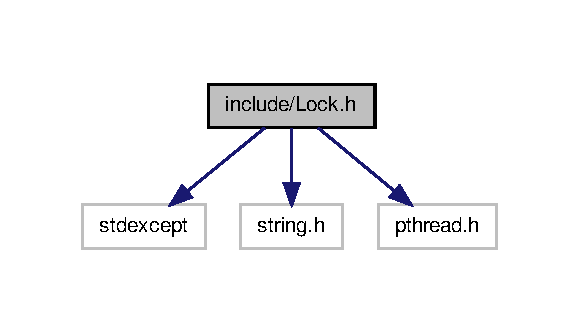
\includegraphics[width=200pt]{_lock_8h__incl}
\end{center}
\end{figure}
\-This graph shows which files directly or indirectly include this file\-:
\nopagebreak
\begin{figure}[H]
\begin{center}
\leavevmode
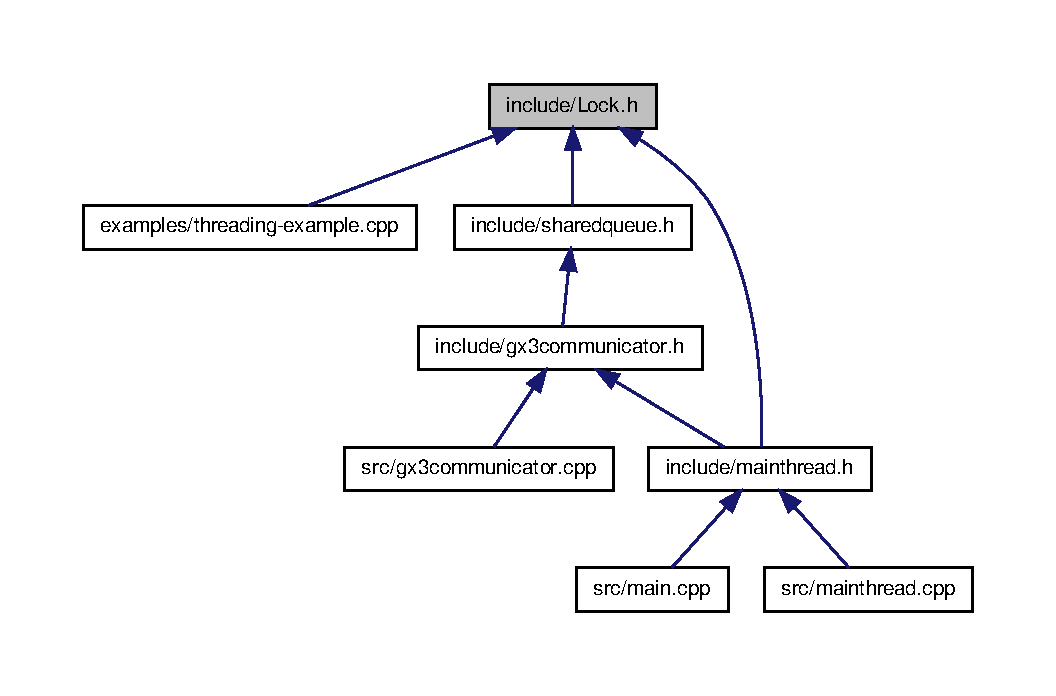
\includegraphics[width=350pt]{_lock_8h__dep__incl}
\end{center}
\end{figure}
\subsection*{\-Classes}
\begin{DoxyCompactItemize}
\item 
class \hyperlink{class_u_s_u_1_1_lock}{\-U\-S\-U\-::\-Lock}
\begin{DoxyCompactList}\small\item\em \-Wrapper class for pthread mutexes. \end{DoxyCompactList}\item 
class \hyperlink{class_u_s_u_1_1_scoped_lock}{\-U\-S\-U\-::\-Scoped\-Lock}
\begin{DoxyCompactList}\small\item\em \-Provides a helper class for \-Scoped \-Mutexes. \end{DoxyCompactList}\end{DoxyCompactItemize}
\subsection*{\-Namespaces}
\begin{DoxyCompactItemize}
\item 
namespace \hyperlink{namespace_u_s_u}{\-U\-S\-U}
\begin{DoxyCompactList}\small\item\em \-T\-O\-D\-O\-: \-Make some proper exceptions. \end{DoxyCompactList}\end{DoxyCompactItemize}


\subsection{\-Detailed \-Description}
\-Small \-C++ wrapper classes for pthread mutexes

\begin{DoxyAuthor}{\-Author}
\-Jan \-Sommer \-Created on\-: \-Apr 10, 2013 
\end{DoxyAuthor}


\-Definition in file \hyperlink{_lock_8h_source}{\-Lock.\-h}.


\hypertarget{periodicrtthread_8cpp}{\section{src/periodicrtthread.cpp \-File \-Reference}
\label{periodicrtthread_8cpp}\index{src/periodicrtthread.\-cpp@{src/periodicrtthread.\-cpp}}
}
{\ttfamily \#include $<$time.\-h$>$}\*
{\ttfamily \#include $<$sys/timerfd.\-h$>$}\*
{\ttfamily \#include $<$stdio.\-h$>$}\*
{\ttfamily \#include $<$unistd.\-h$>$}\*
{\ttfamily \#include $<$cerrno$>$}\*
{\ttfamily \#include \char`\"{}periodicrtthread.\-h\char`\"{}}\*
\-Include dependency graph for periodicrtthread.\-cpp\-:\nopagebreak
\begin{figure}[H]
\begin{center}
\leavevmode
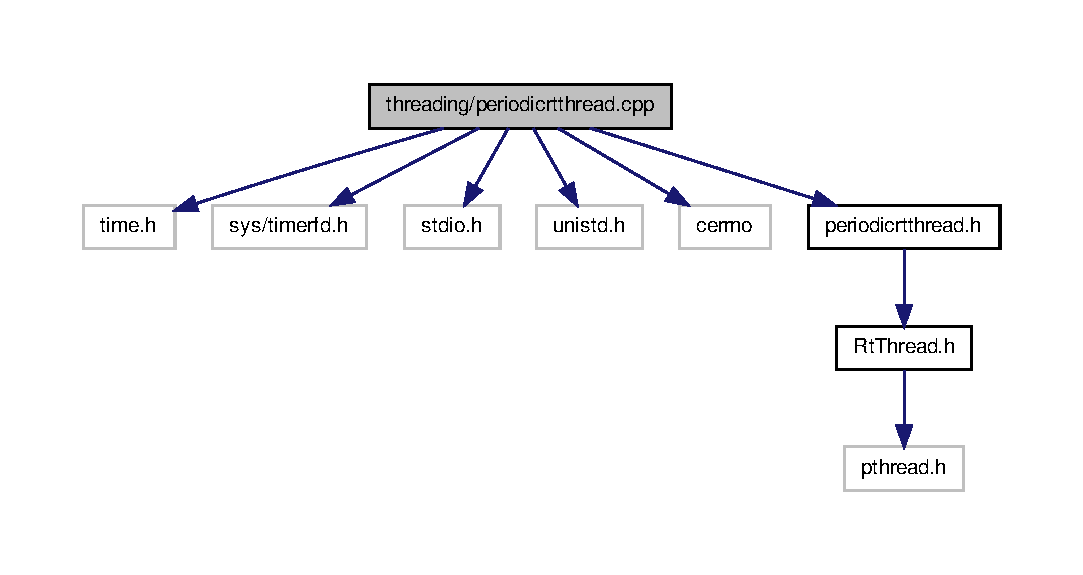
\includegraphics[width=350pt]{periodicrtthread_8cpp__incl}
\end{center}
\end{figure}


\subsection{\-Detailed \-Description}
\-Small \-C++ wrapper class to create a realtime scheduled pthread with periodic timer events.

\begin{DoxyAuthor}{\-Author}
\-Jan \-Sommer \-Created on\-: \-Apr 10, 2013 
\end{DoxyAuthor}


\-Definition in file \hyperlink{periodicrtthread_8cpp_source}{periodicrtthread.\-cpp}.


\hypertarget{periodicrtthread_8h}{\section{include/periodicrtthread.h \-File \-Reference}
\label{periodicrtthread_8h}\index{include/periodicrtthread.\-h@{include/periodicrtthread.\-h}}
}
{\ttfamily \#include \char`\"{}\-Rt\-Thread.\-h\char`\"{}}\*
\-Include dependency graph for periodicrtthread.\-h\-:\nopagebreak
\begin{figure}[H]
\begin{center}
\leavevmode
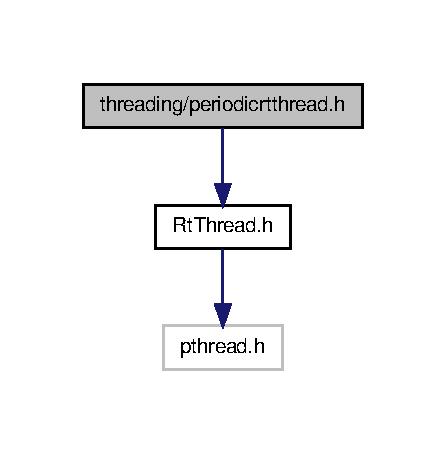
\includegraphics[width=214pt]{periodicrtthread_8h__incl}
\end{center}
\end{figure}
\-This graph shows which files directly or indirectly include this file\-:\nopagebreak
\begin{figure}[H]
\begin{center}
\leavevmode
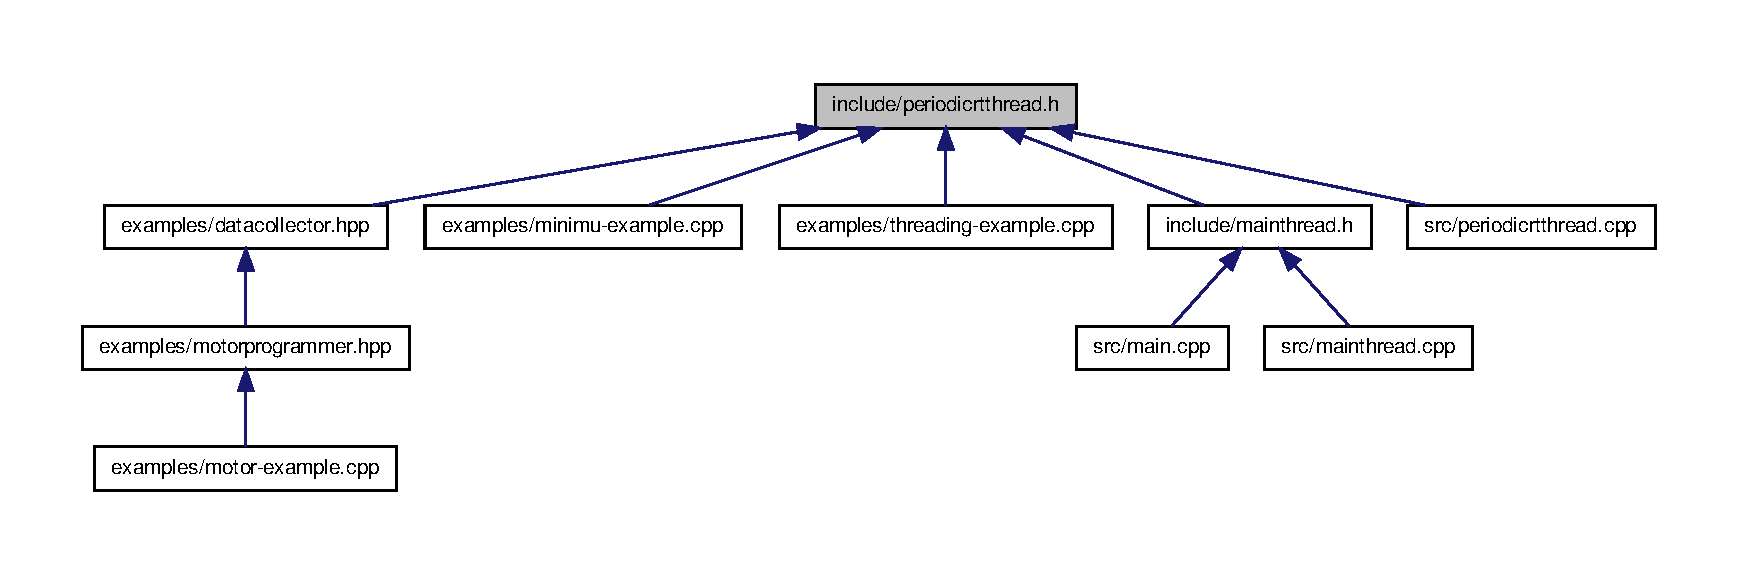
\includegraphics[width=350pt]{periodicrtthread_8h__dep__incl}
\end{center}
\end{figure}
\subsection*{\-Classes}
\begin{DoxyCompactItemize}
\item 
class \hyperlink{class_u_s_u_1_1_periodic_rt_thread}{\-U\-S\-U\-::\-Periodic\-Rt\-Thread}
\begin{DoxyCompactList}\small\item\em \-T\-O\-D\-O\-: \-Make some proper exceptions. \end{DoxyCompactList}\end{DoxyCompactItemize}
\subsection*{\-Namespaces}
\begin{DoxyCompactItemize}
\item 
namespace \hyperlink{namespace_u_s_u}{\-U\-S\-U}
\begin{DoxyCompactList}\small\item\em \-T\-O\-D\-O\-: \-Make some proper exceptions. \end{DoxyCompactList}\end{DoxyCompactItemize}


\subsection{\-Detailed \-Description}
\-Small \-C++ wrapper class to create a realtime scheduled pthread with periodic timer events.

\begin{DoxyAuthor}{\-Author}
\-Jan \-Sommer \-Created on\-: \-Apr 10, 2013 
\end{DoxyAuthor}


\-Definition in file \hyperlink{periodicrtthread_8h_source}{periodicrtthread.\-h}.


\hypertarget{_rt_thread_8cpp}{\subsection{src/\-Rt\-Thread.cpp \-File \-Reference}
\label{_rt_thread_8cpp}\index{src/\-Rt\-Thread.\-cpp@{src/\-Rt\-Thread.\-cpp}}
}
{\ttfamily \#include $<$stdio.\-h$>$}\*
{\ttfamily \#include $<$time.\-h$>$}\*
{\ttfamily \#include $<$errno.\-h$>$}\*
{\ttfamily \#include \char`\"{}\-Rt\-Thread.\-h\char`\"{}}\*
\-Include dependency graph for \-Rt\-Thread.\-cpp\-:\nopagebreak
\begin{figure}[H]
\begin{center}
\leavevmode
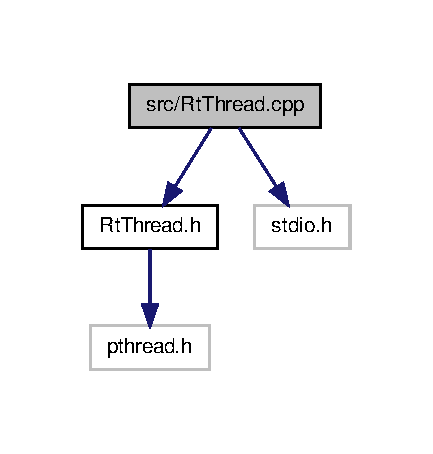
\includegraphics[width=334pt]{_rt_thread_8cpp__incl}
\end{center}
\end{figure}


\subsubsection{\-Detailed \-Description}
\-Small \-C++ wrapper class to create a realtime scheduled pthread

\begin{DoxyAuthor}{\-Author}
\-Jan \-Sommer \-Created on\-: \-Apr 10, 2013 
\end{DoxyAuthor}


\-Definition in file \hyperlink{_rt_thread_8cpp_source}{\-Rt\-Thread.\-cpp}.


\hypertarget{_rt_thread_8h}{\section{threading/\-Rt\-Thread.h \-File \-Reference}
\label{_rt_thread_8h}\index{threading/\-Rt\-Thread.\-h@{threading/\-Rt\-Thread.\-h}}
}
{\ttfamily \#include $<$pthread.\-h$>$}\*
\-Include dependency graph for \-Rt\-Thread.\-h\-:
\nopagebreak
\begin{figure}[H]
\begin{center}
\leavevmode
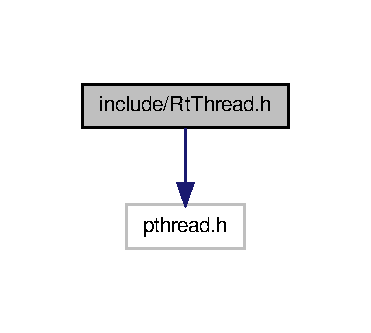
\includegraphics[width=188pt]{_rt_thread_8h__incl}
\end{center}
\end{figure}
\-This graph shows which files directly or indirectly include this file\-:
\nopagebreak
\begin{figure}[H]
\begin{center}
\leavevmode
\includegraphics[width=350pt]{_rt_thread_8h__dep__incl}
\end{center}
\end{figure}
\subsection*{\-Classes}
\begin{DoxyCompactItemize}
\item 
class \hyperlink{class_u_s_u_1_1_rt_thread}{\-U\-S\-U\-::\-Rt\-Thread}
\begin{DoxyCompactList}\small\item\em \-Abstract wrapper class for the pthread library with \-R\-T-\/priority. \end{DoxyCompactList}\end{DoxyCompactItemize}
\subsection*{\-Namespaces}
\begin{DoxyCompactItemize}
\item 
namespace \hyperlink{namespace_u_s_u}{\-U\-S\-U}
\begin{DoxyCompactList}\small\item\em \-T\-O\-D\-O\-: \-Make some proper exceptions. \end{DoxyCompactList}\end{DoxyCompactItemize}


\subsection{\-Detailed \-Description}
\-Small \-C++ wrapper class to create a realtime scheduled pthread

\begin{DoxyAuthor}{\-Author}
\-Jan \-Sommer \-Created on\-: \-Apr 10, 2013 
\end{DoxyAuthor}


\-Definition in file \hyperlink{_rt_thread_8h_source}{\-Rt\-Thread.\-h}.


\printindex
\end{document}
